\documentclass[t]{beamer}
\usepackage{amsmath}
\usepackage{amsthm}
\usepackage[T1]{fontenc}
\usepackage{lmodern}
\usepackage{color}
\usepackage{xcolor}
\usepackage{hyperref}
\usepackage{multirow,varwidth} % used for SL table
\usepackage{tikz}
\usepackage{multicol}
\usepackage{graphicx}
\usepackage{etoolbox}
\usepackage{bm}
\usepackage[abs]{overpic}
\usepackage{pict2e}
\usepackage{animate}
\usepackage{verbatim}
\usepackage{soul}
\usepackage{xmpmulti}
\usepackage{subfig}
\usepackage{media9}
\usepackage{appendixnumberbeamer}

\usetheme{PaloAlto}
\usecolortheme{seahorse}
% \usecolortheme{spruce}

\newenvironment{withoutheadline}{
\setlength{\headheight}{0pt}
\setbeamertemplate{headline}{}}

\setbeamercolor*{block title example}{fg=white,
bg= black!30!blue}
\setbeamercolor*{block body example}{fg=black,
bg= blue!5}

\setbeamertemplate{frametitle continuation}{}

\setbeamertemplate{footline}{}

\setbeamertemplate{itemize items}[circle]
\setbeamertemplate{navigation symbols}[only frame symbol]
\setbeamerfont{framesubtitle}{size=\large}


\title{{\bf Targeted Learning}}
\subtitle{Bridging Machine Learning with Causal and Statistical Inference}
\author{Mark van der Laan\inst{1} and Nima Hejazi\inst{2}}

\institute{
\inst{1} Division of Biostatistics, University of California, Berkeley \and
\inst{2} Department of Biostatistics, Harvard T.H.~Chan School of Public Health
}

\date{
15\textsuperscript{th} November 2024\\[2pt]
Harvard Catalyst Workshop
\\[2pt]
{\tiny Acknowledgements: Susan Gruber, Alan Hubbard, Ivana Malenica, Rachael
Phillips, Lars van der Laan}
}

\begin{document}

\begin{frame}[noframenumbering]
\titlepage
\end{frame}

\section{The Art of Statistics}

\begin{frame}
\frametitle{A traditional toolbox for statistics}
\vspace{-12pt}
\centering
\begin{figure}
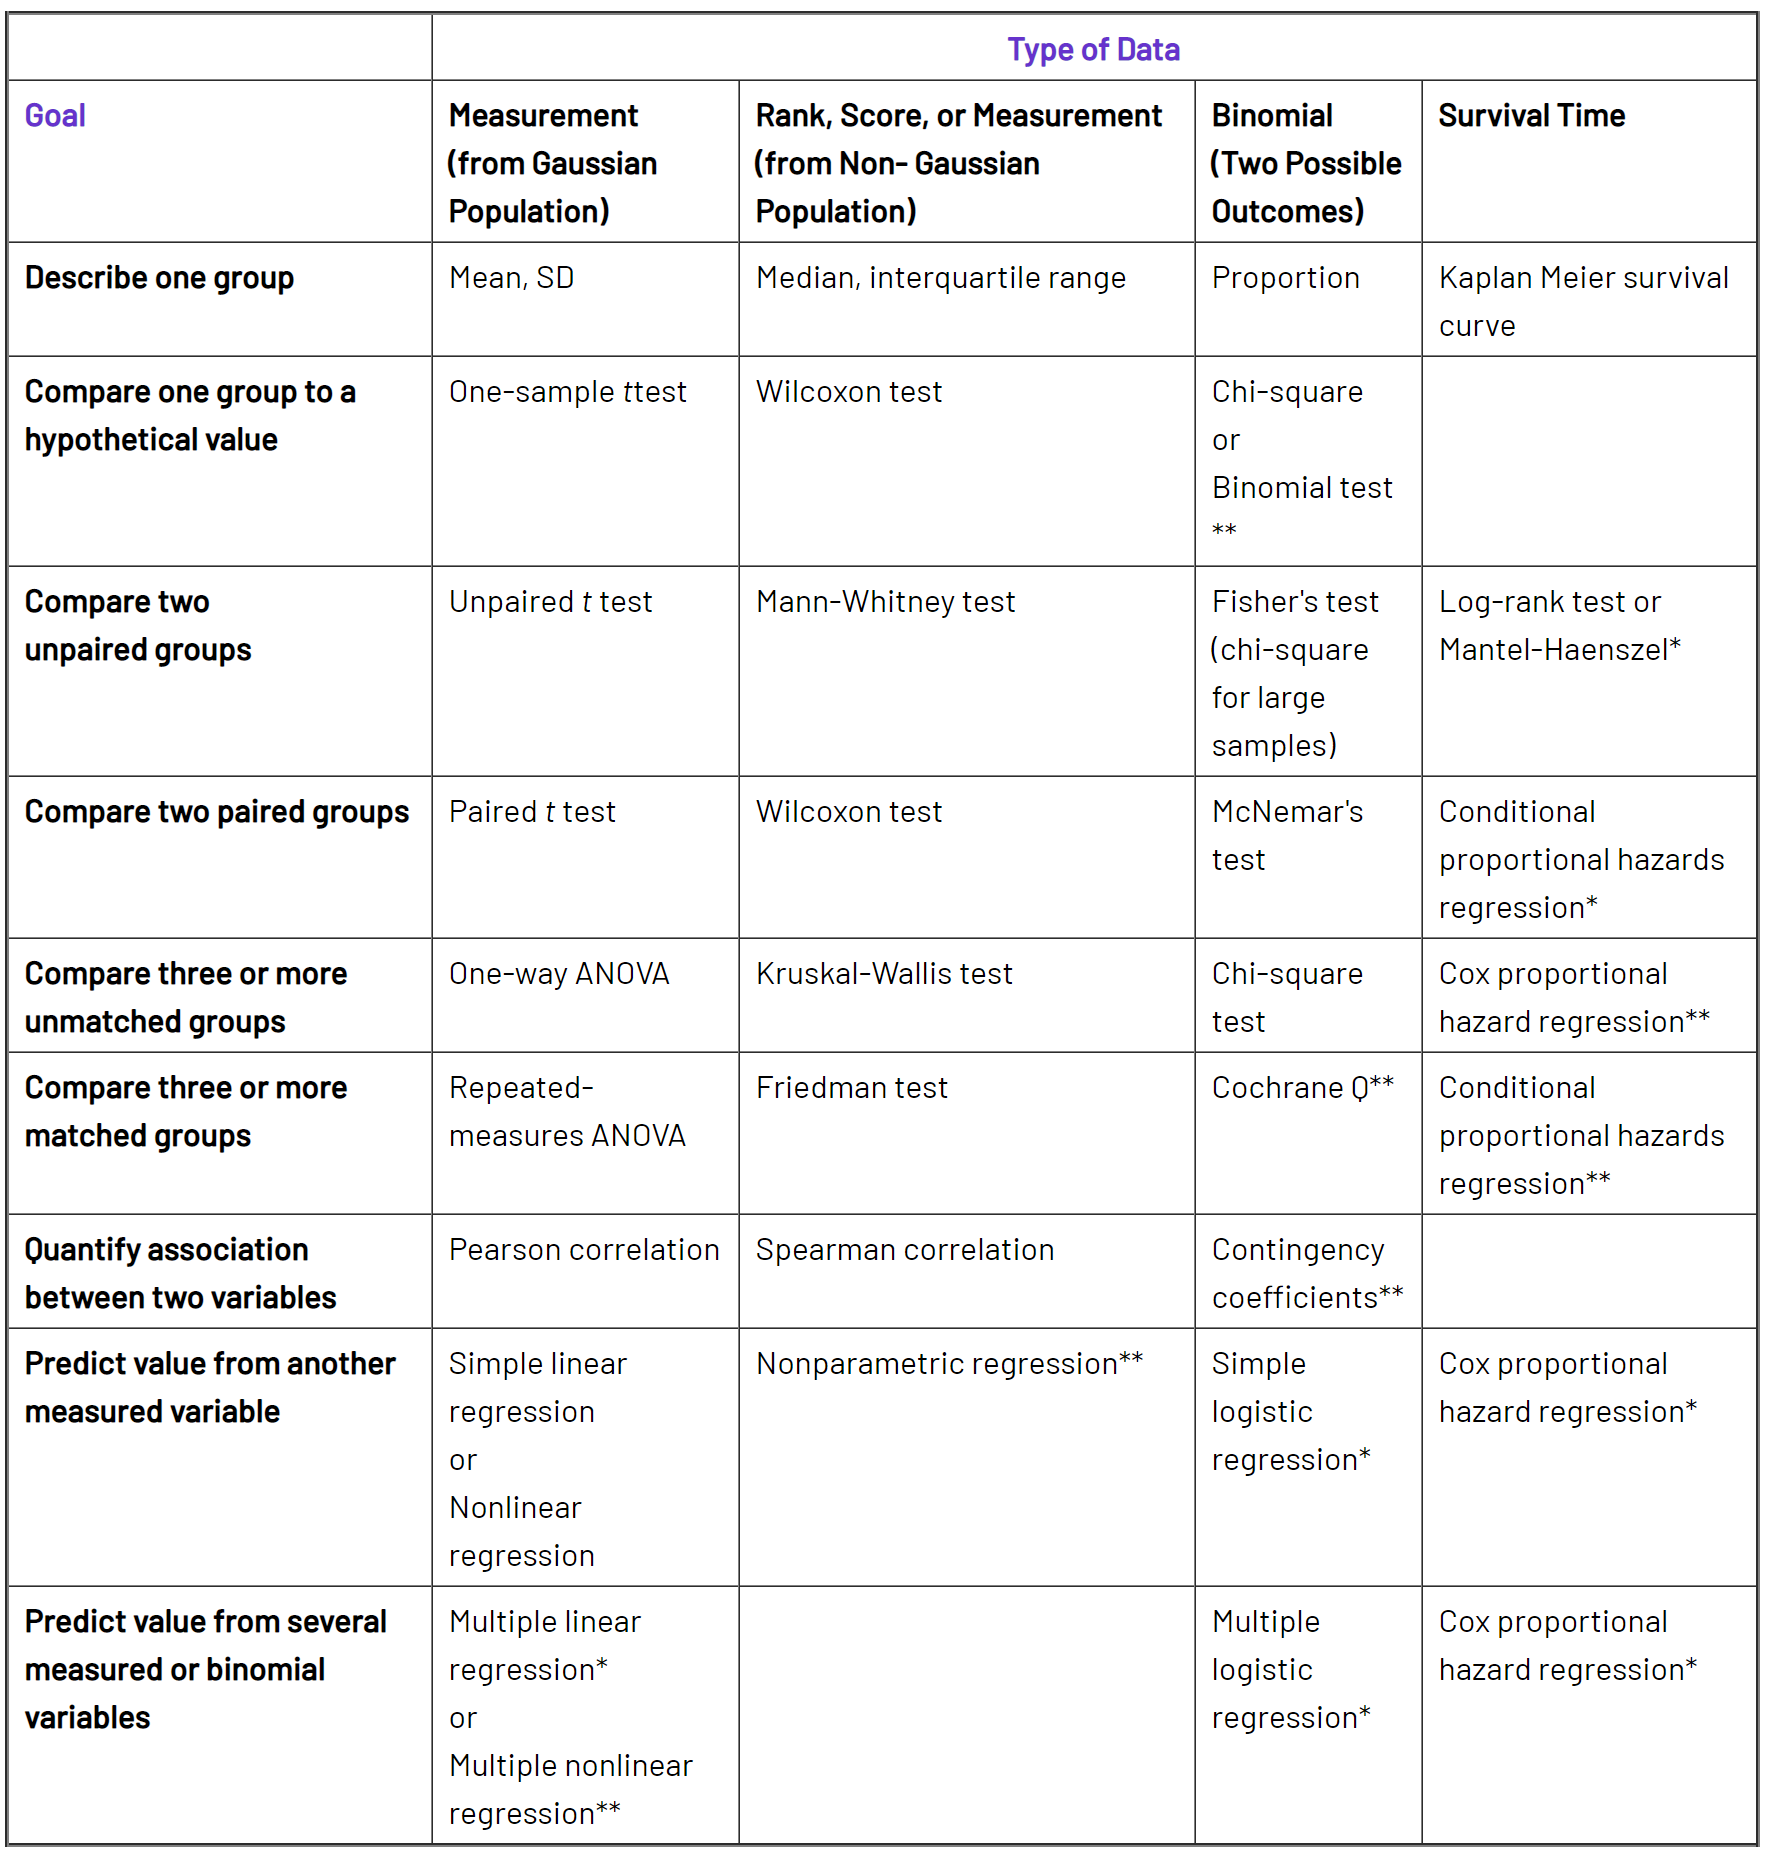
\includegraphics[width=0.73\textwidth]{figures/statistics-for-dummies.png}
% Source: https://www.graphpad.com/support/faqid/1790/
\end{figure}
\end{frame}

% \begin{frame}
% \frametitle{A traditional toolbox for statistics}
% \vspace{-12pt}
% \centering
% \begin{figure}
% 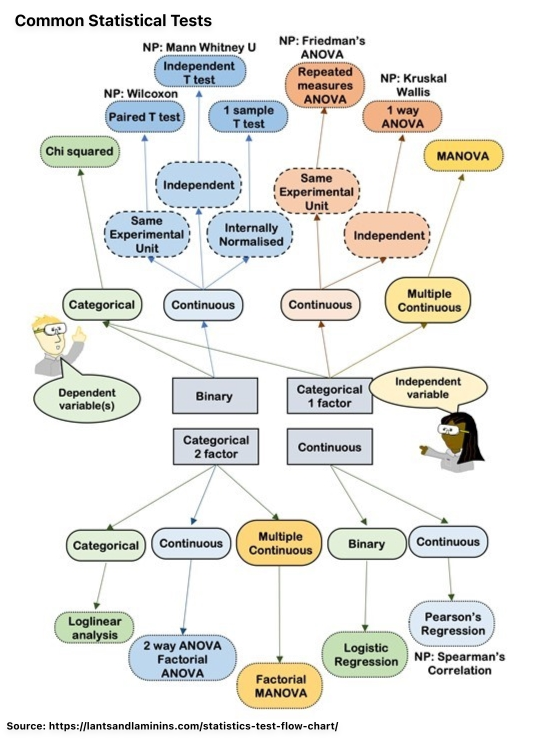
\includegraphics[width=0.5\textwidth]{figures/stat-tests.png}
% % Source: https://www.graphpad.com/support/faqid/1790/
% \end{figure}
% \end{frame}

\begin{frame}
\frametitle{A traditional toolbox for statistics}
\vspace{-12pt}
\centering
\begin{figure}
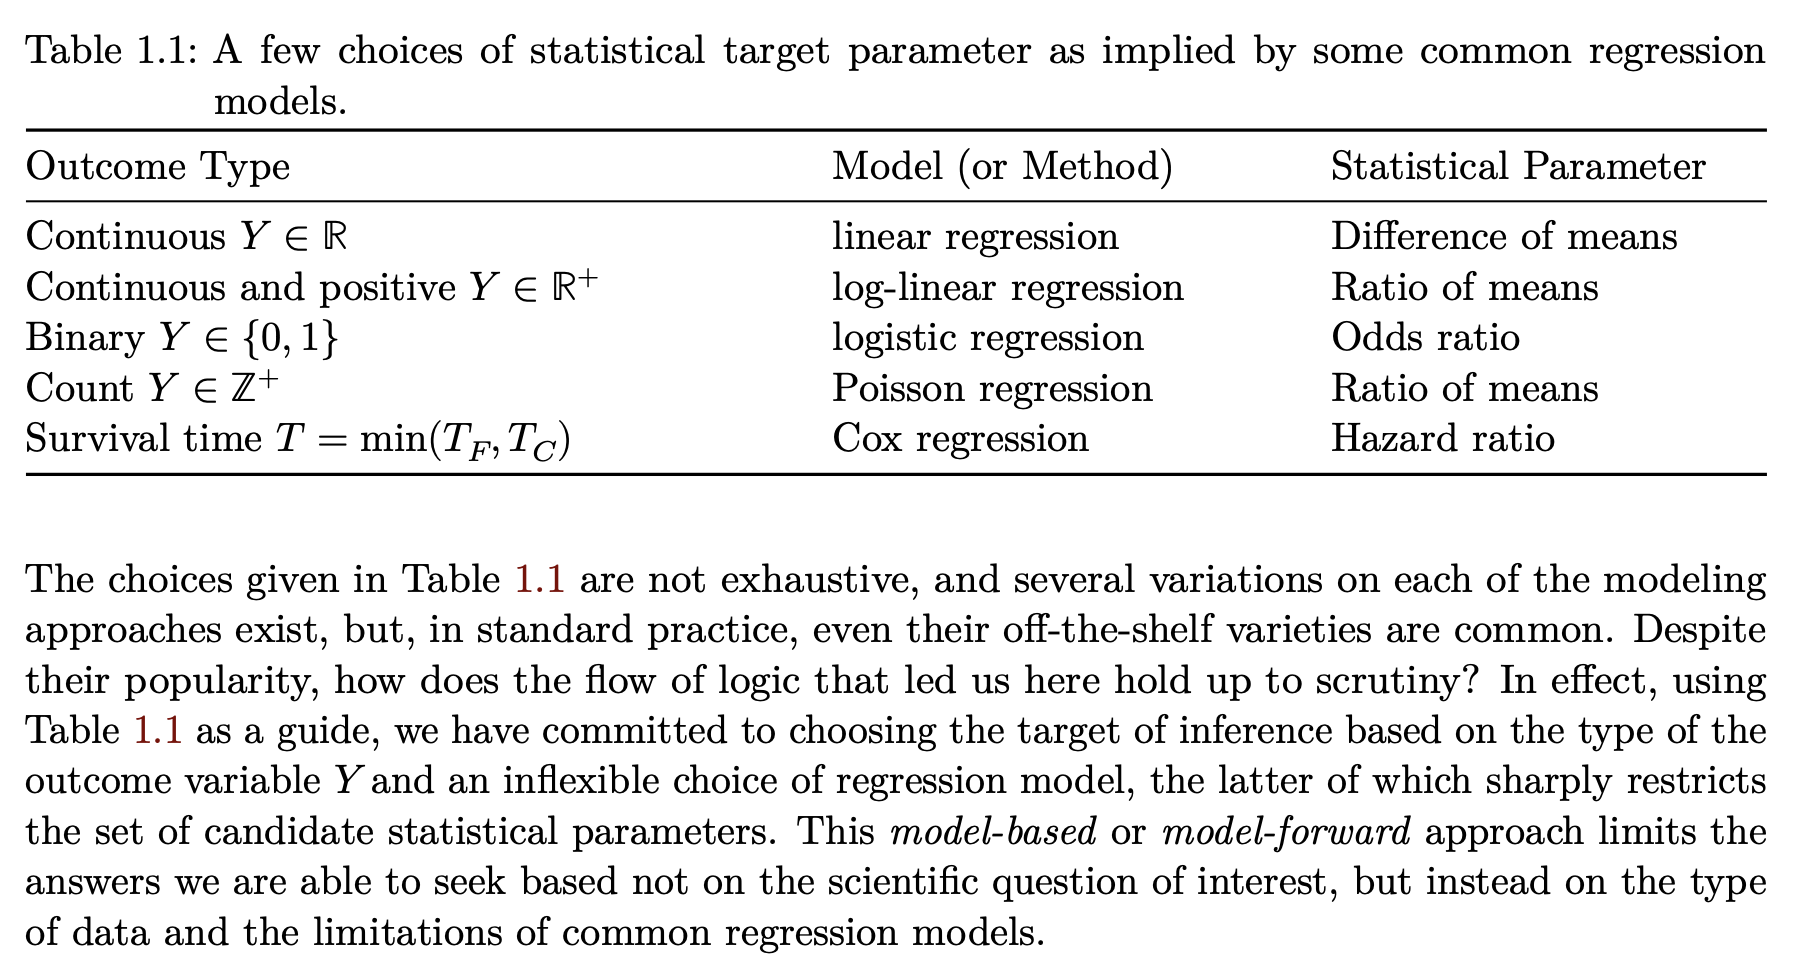
\includegraphics[width=0.9\textwidth]{figures/parametric.png}
\vspace{1em}
\begin{itemize}
  \item Traditional: Data $+$ Model $\rightarrow$ Question (parameter)
  \item Agnostic: Question (parameter) $+$ Data $\rightarrow$ Model
  \item Which of these is better aligned with the scientific process?
\end{itemize}
\end{figure}

\end{frame}
\begin{frame}
\frametitle{Performance of traditional tools}
\vspace{5pt}
\centering
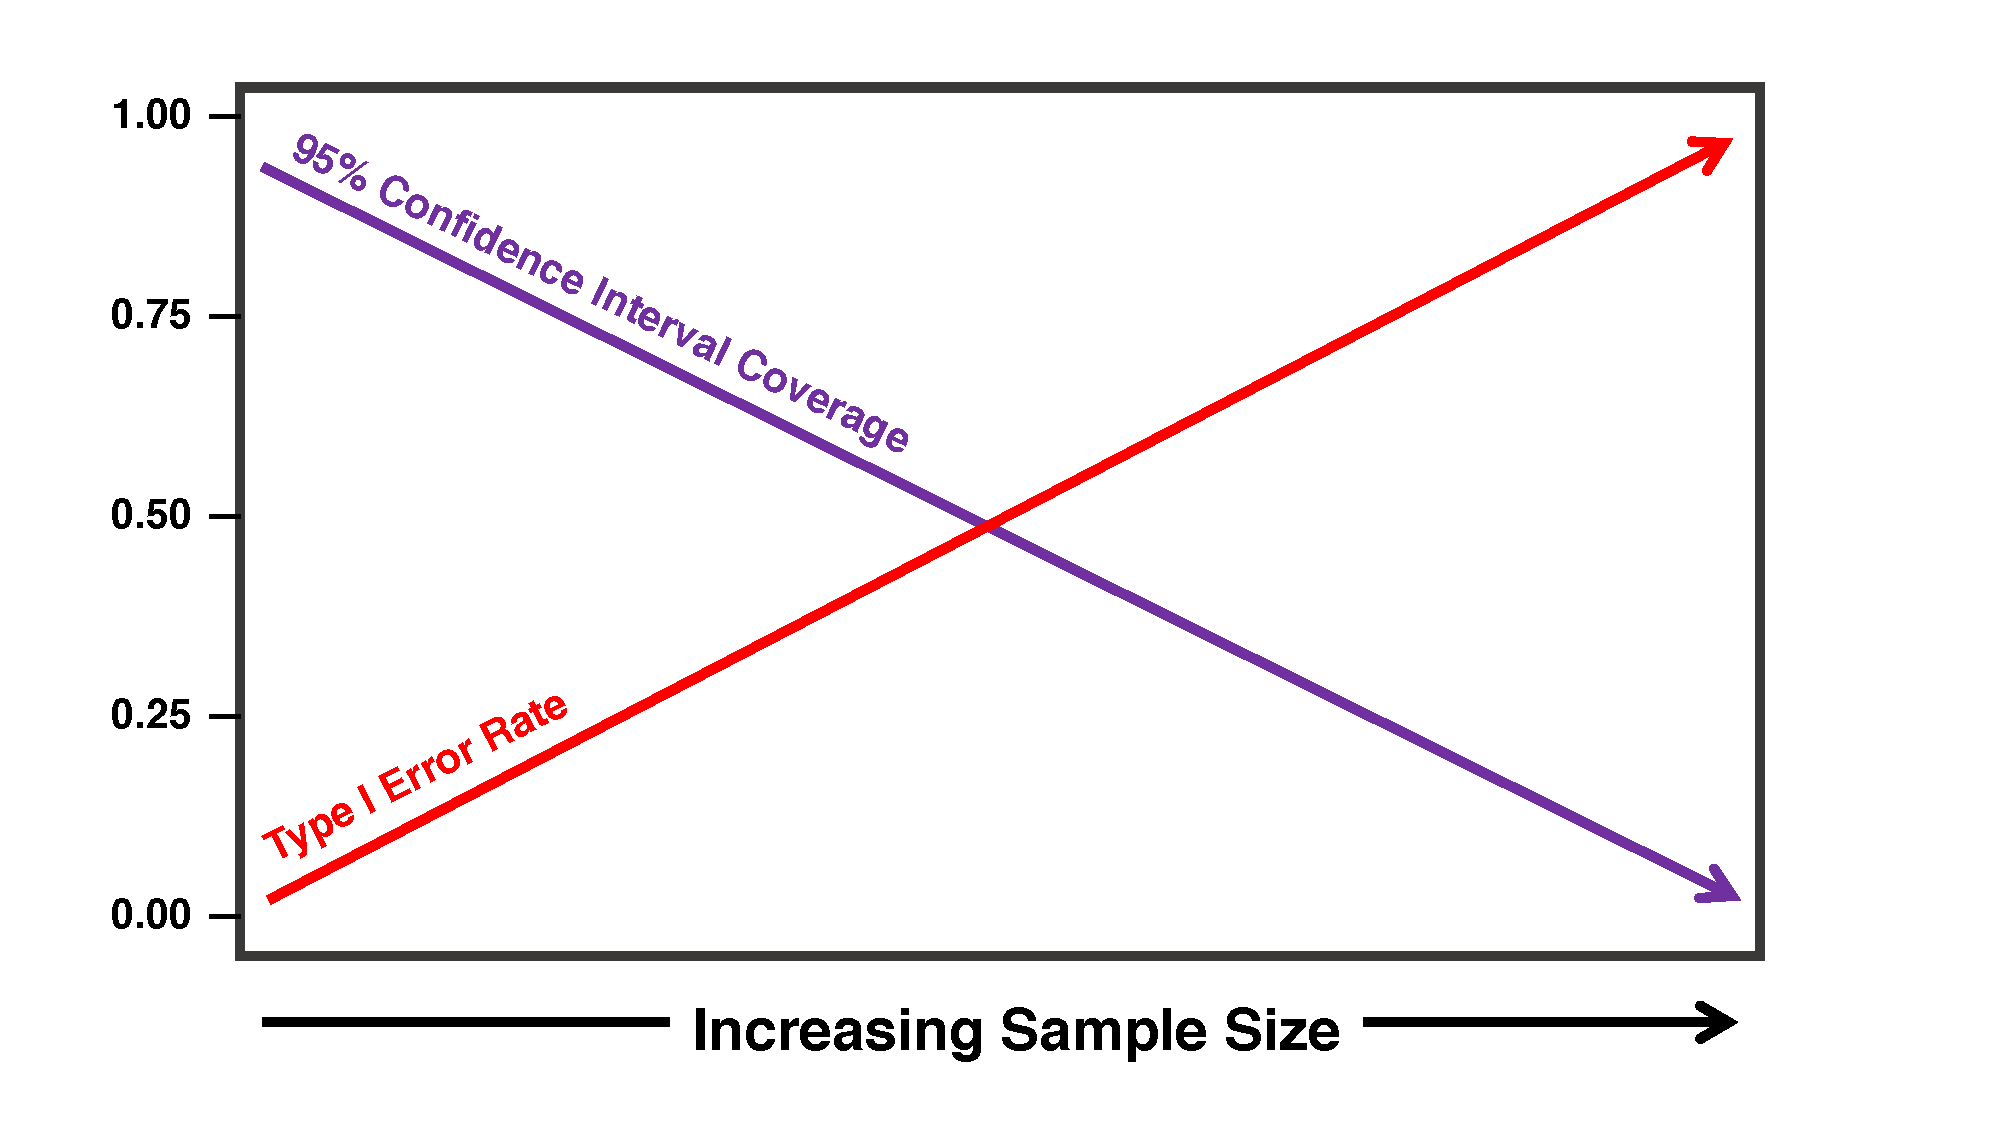
\includegraphics[width=1.05\textwidth]{figures/misspecified.pdf}
\end{frame}

\begin{frame}
\frametitle{Performance of traditional tools}
\vspace{5pt}
\centering
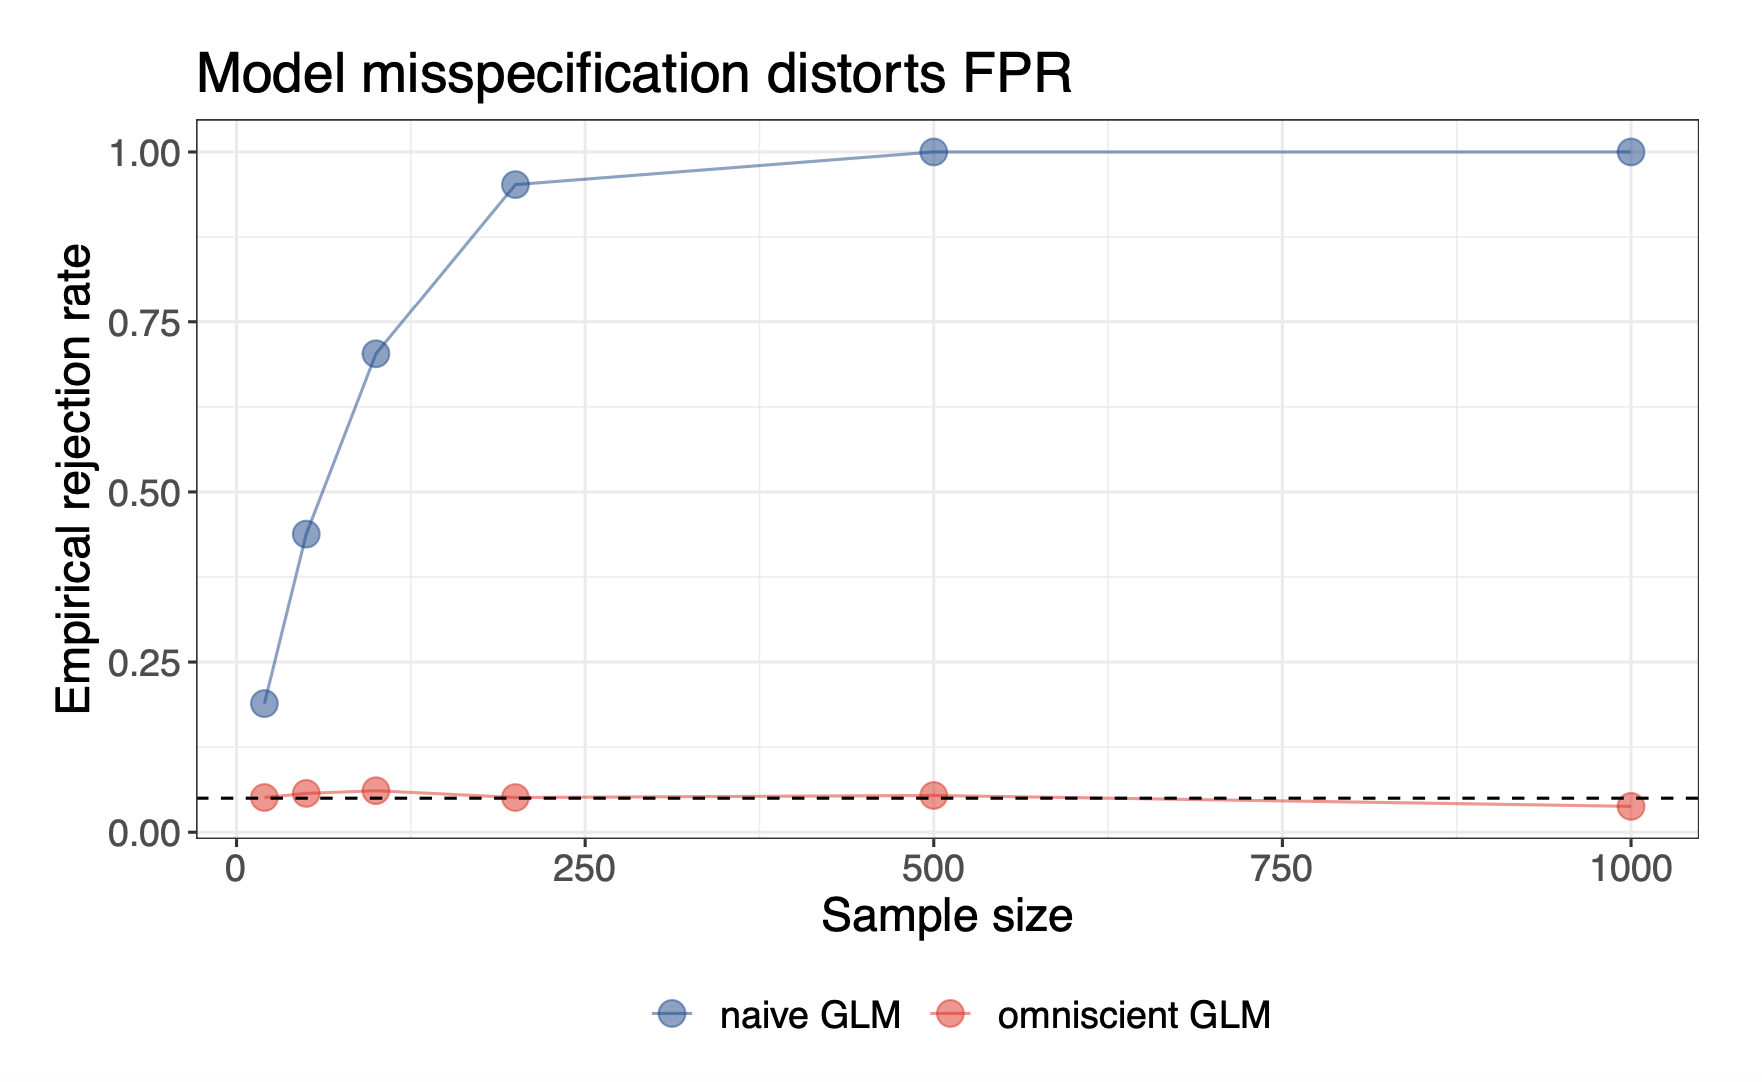
\includegraphics[width=1.0\textwidth]{figures/fpr_bst258.png}
\vspace{0.5em}
Truth: No effect of exposure on outcome.
\end{frame}

% \begin{frame}
% \frametitle{Post-hoc model manipulation}
% \centering
% \vspace{-.11in}
% \begin{figure}
% 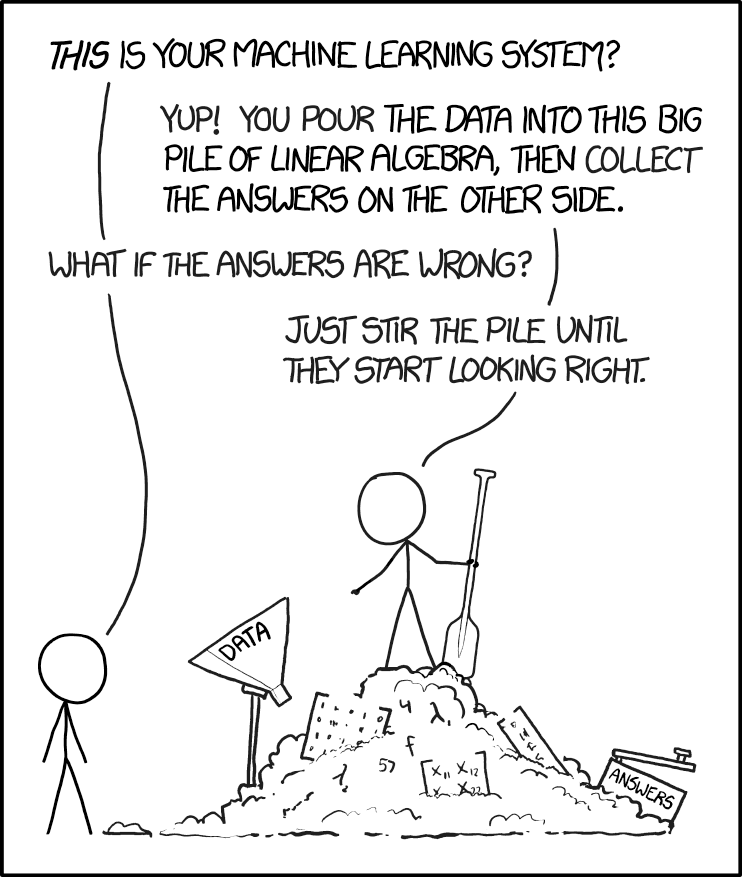
\includegraphics[width=0.62\textwidth]{figures/comic.png}
% \end{figure}
% \end{frame}

\begin{frame}
\frametitle{The ``art'' of statistical inference?}
\vspace{-.2in}
\centering
\begin{figure}
\fbox{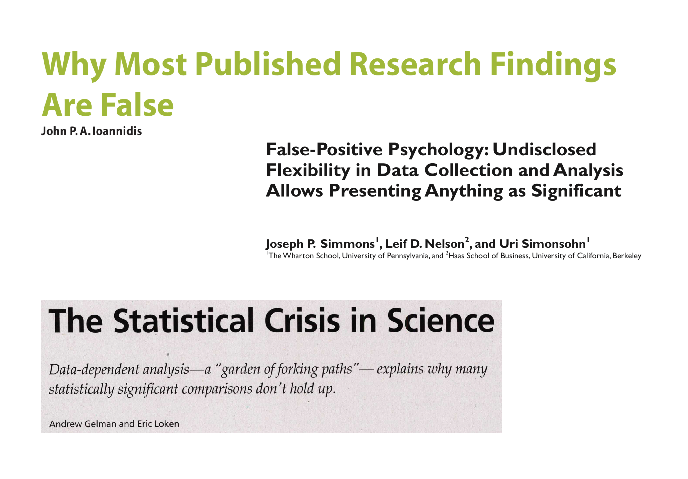
\includegraphics[width=.98\textwidth]{figures/articles.pdf}}
\end{figure}
\end{frame}

\section{TL in Action}

\begin{frame}
  \frametitle{TL answers statistical questions rooted in causality}
  \vspace{-1em}
  \begin{center}
  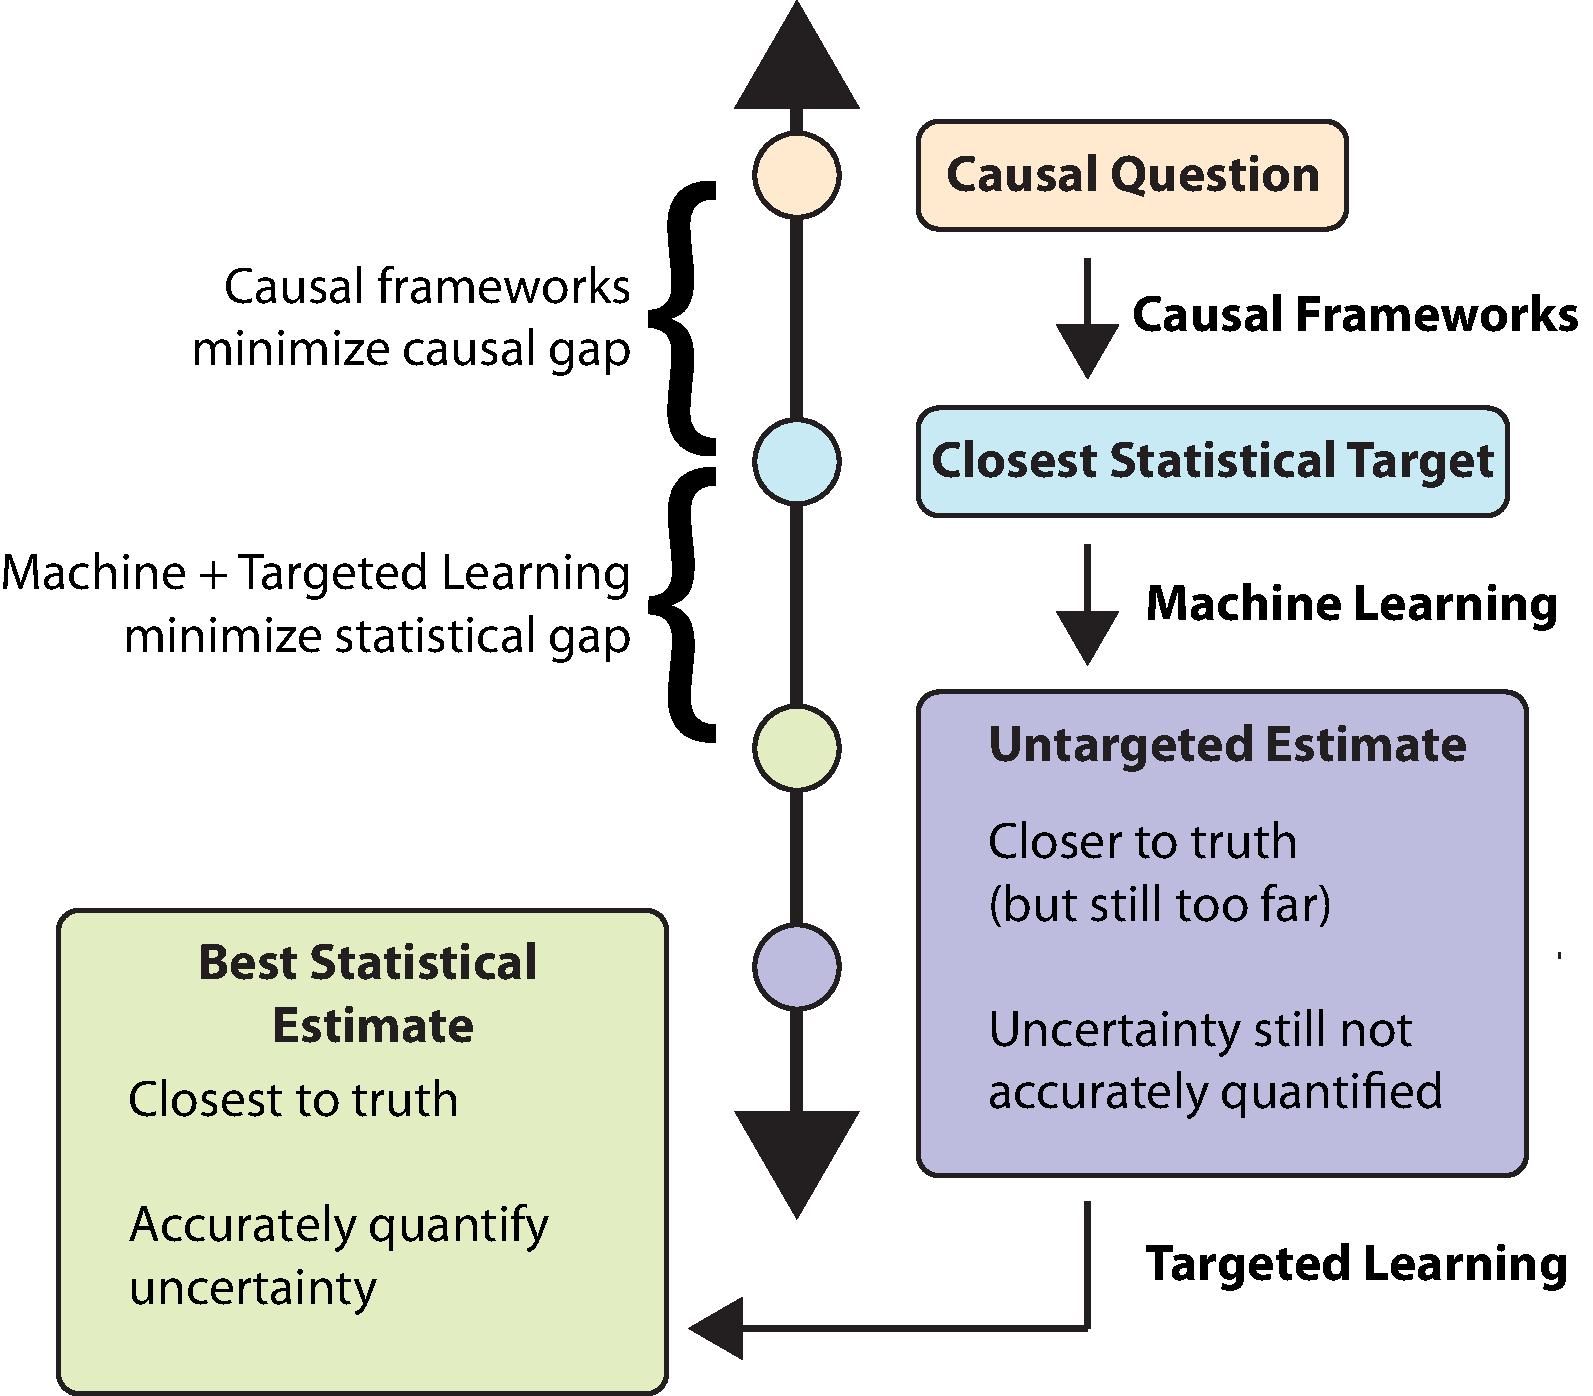
\includegraphics[width=0.84\textwidth]{figures/schematic-fixed.pdf}
  \end{center}
\end{frame}

\begin{frame}
\frametitle{Public health and medicine use real-world data (RWD) for insight
  and evidence}
\vspace{20pt}
\begin{center}
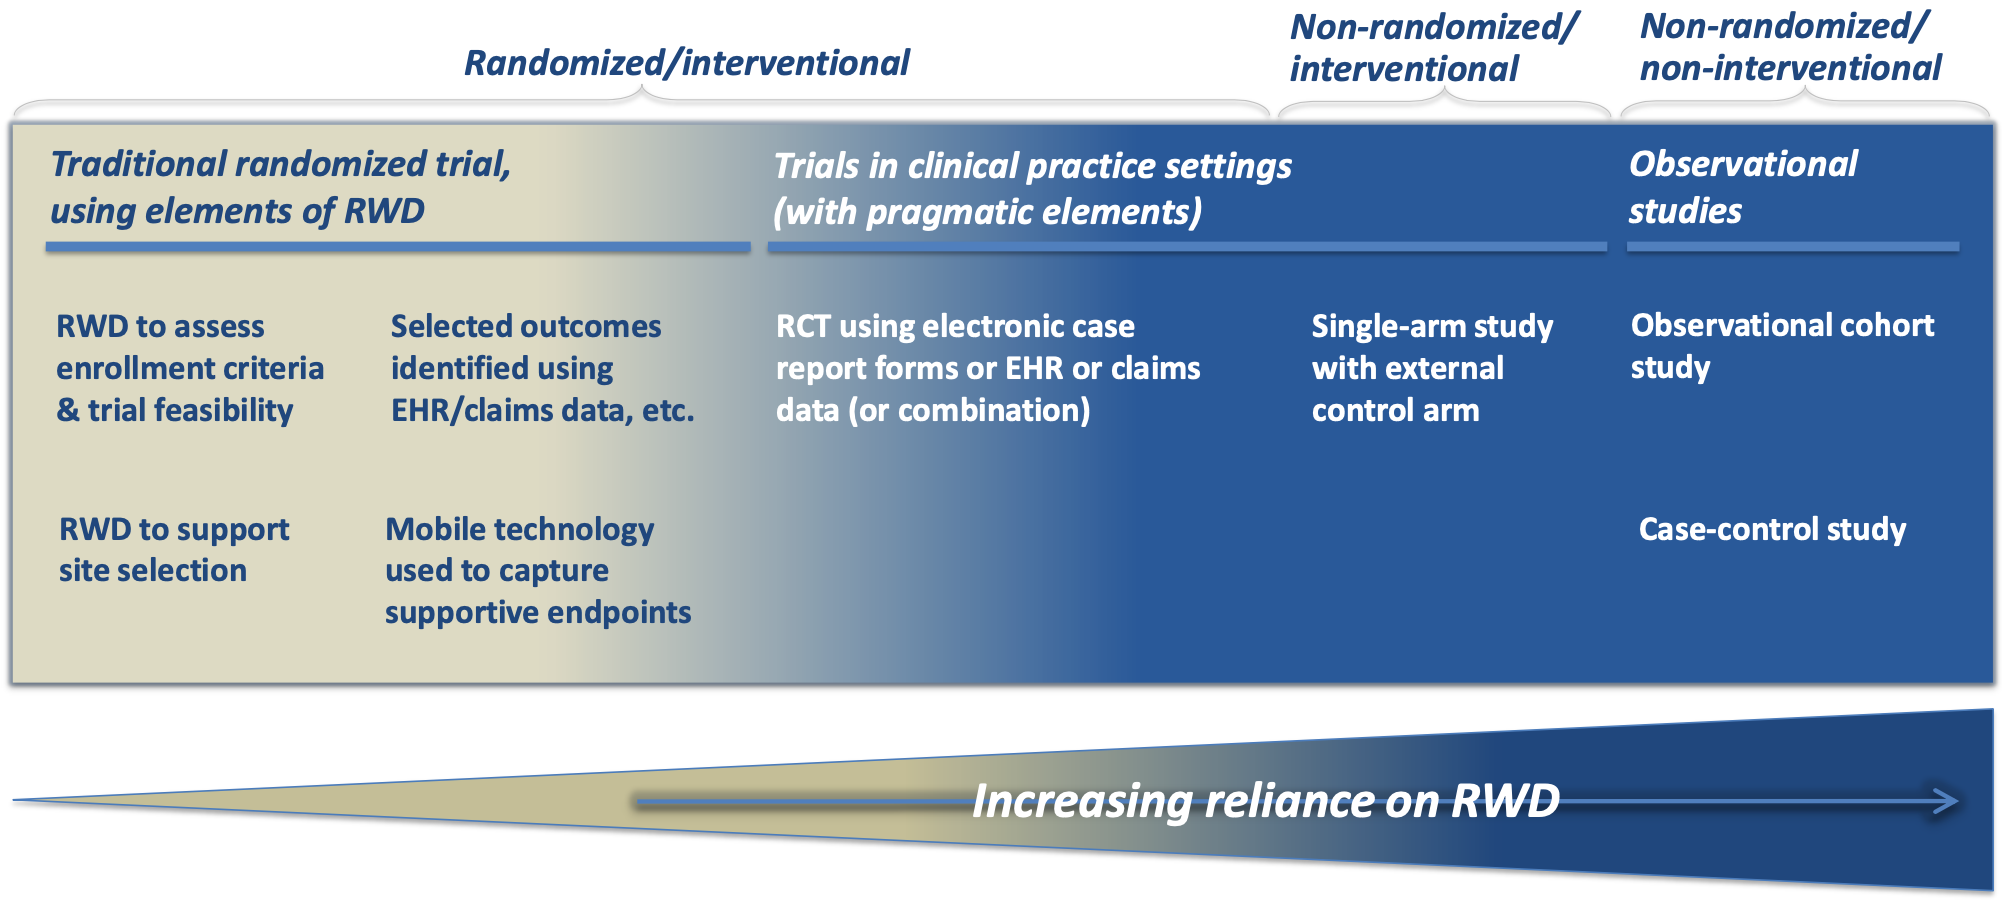
\includegraphics[width=\textwidth]{figures/john_slide8_figure.png}
\end{center}
\vspace{35pt}
\tiny{Courtesy of "FDA Real-World Evidence Program" Webinar by John Concato on
  4\textsuperscript{th} August 2021}
\end{frame}

\begin{frame}
\frametitle{TL addresses statistical challenges with RWD}
\vspace{-18pt}
\begin{center}
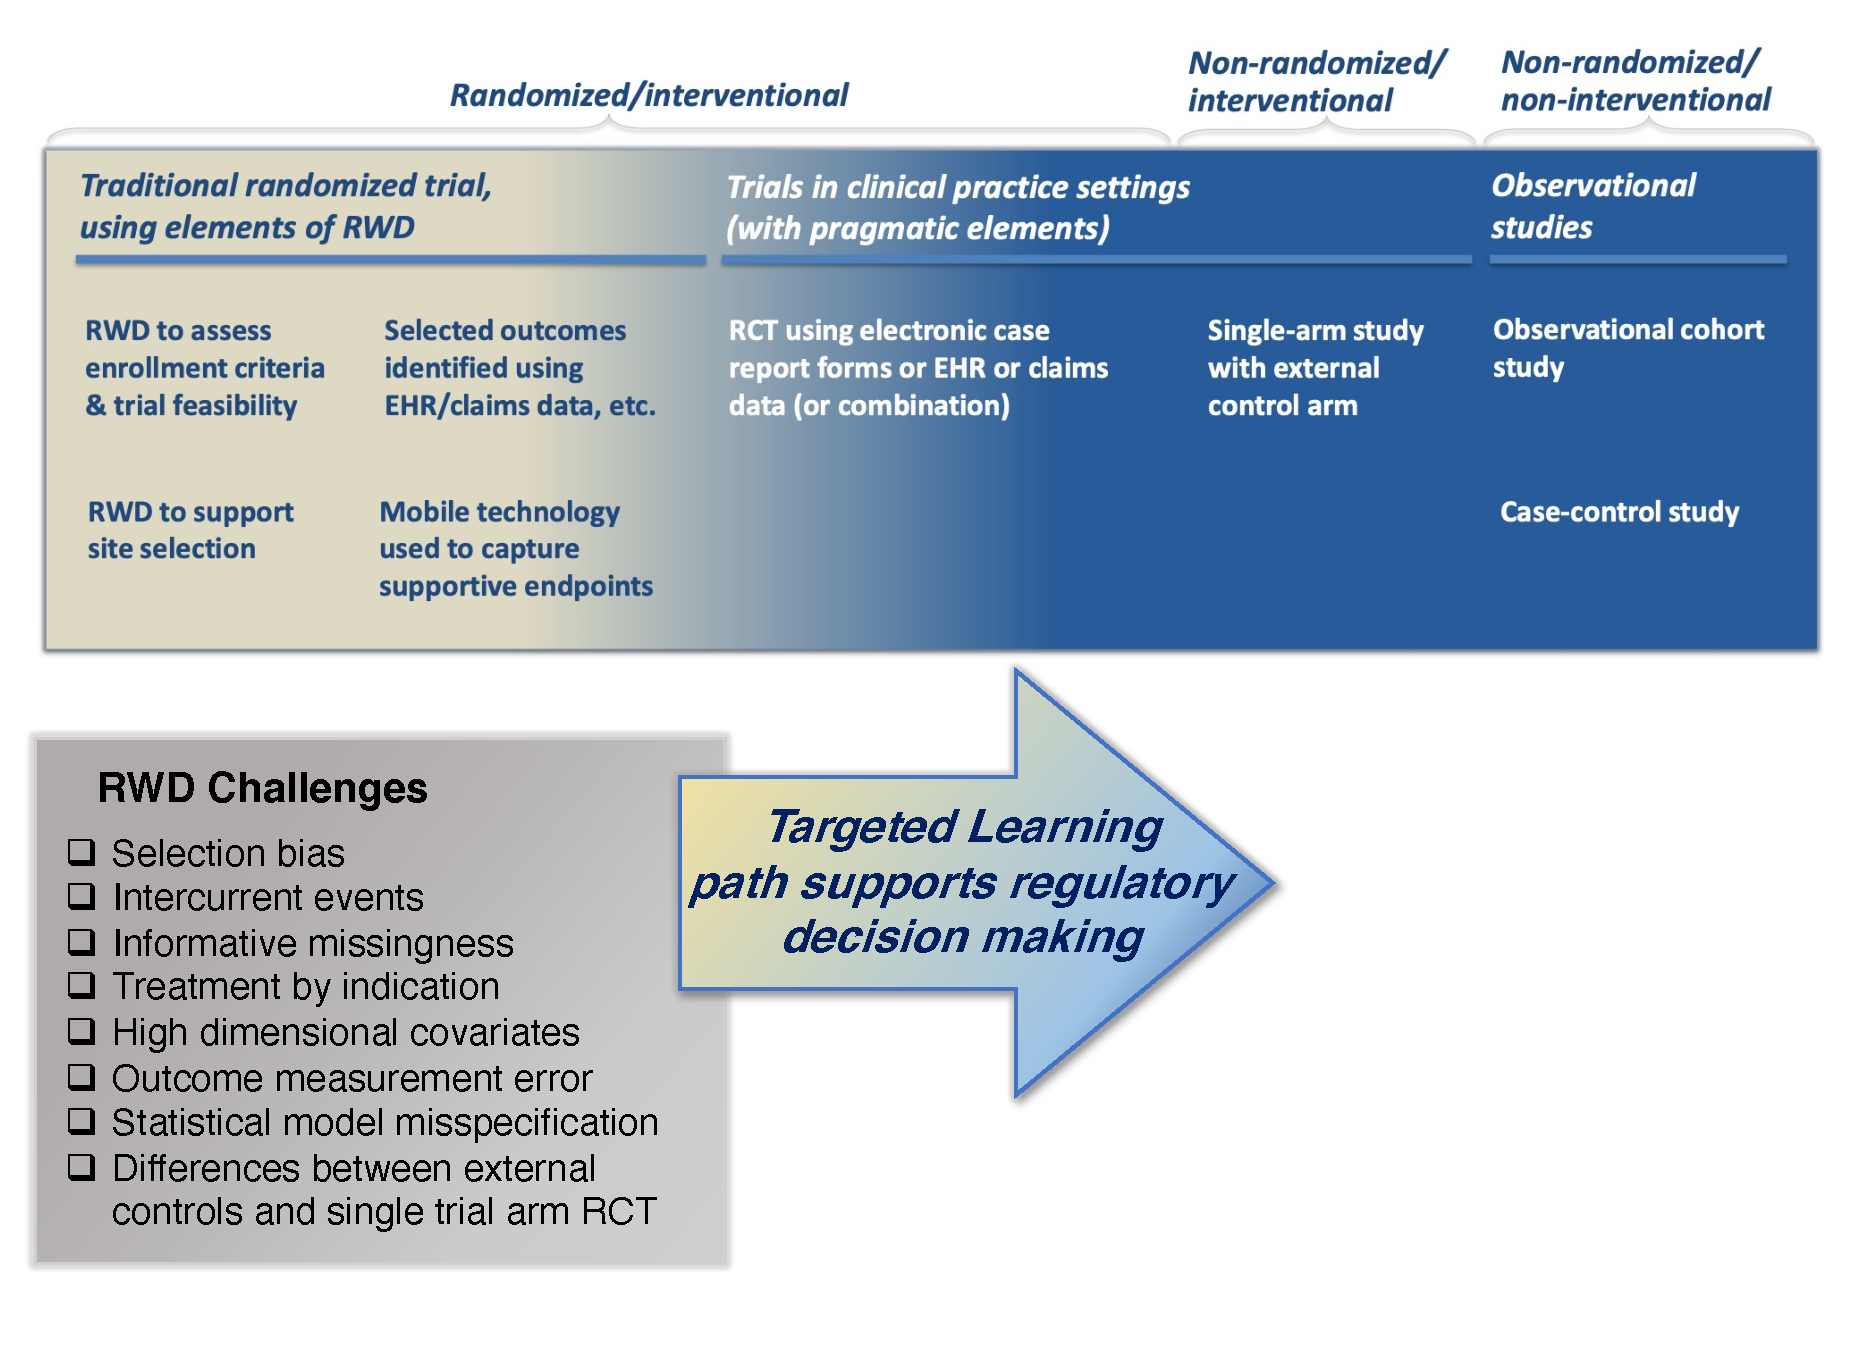
\includegraphics[width=1.02\textwidth]{figures/TLpath1_edit.pdf}
\end{center}
\end{frame}

\begin{frame}
\frametitle{TL for real-world evidence (RWE) evaluation}
\vspace{-18pt}
\centering
\begin{figure}
\begin{center}
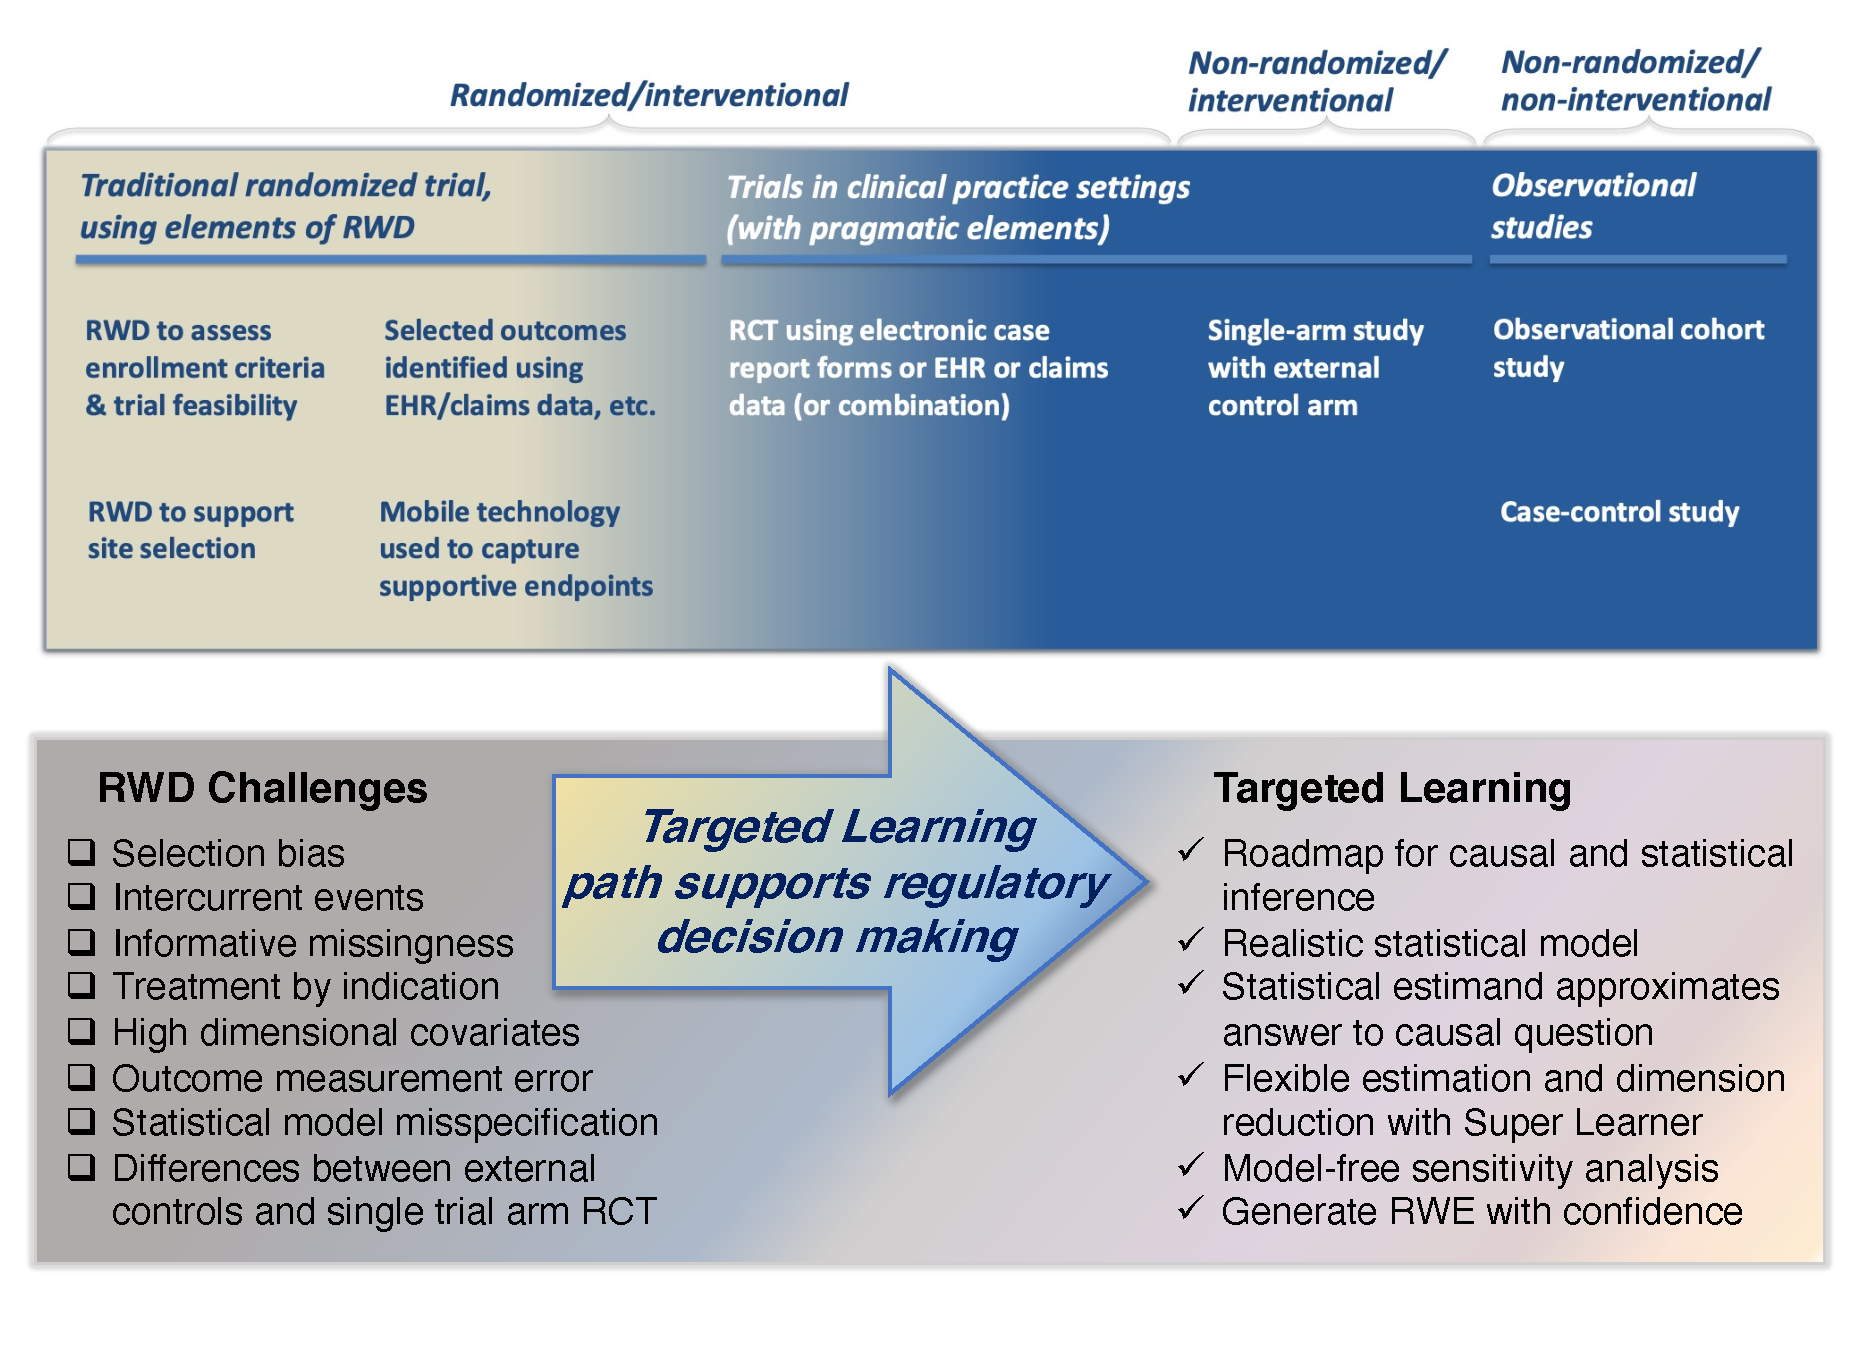
\includegraphics[width=1.02\textwidth]{figures/TLpath2_edit.pdf}
\end{center}
\end{figure}
\vspace{35pt}
\end{frame}

\begin{frame}
\frametitle{TL is a subfield of statistics}
\vspace{-25pt}
\begin{columns}
\begin{column}{4.9cm}
\begin{center}
\begin{figure}
\fbox{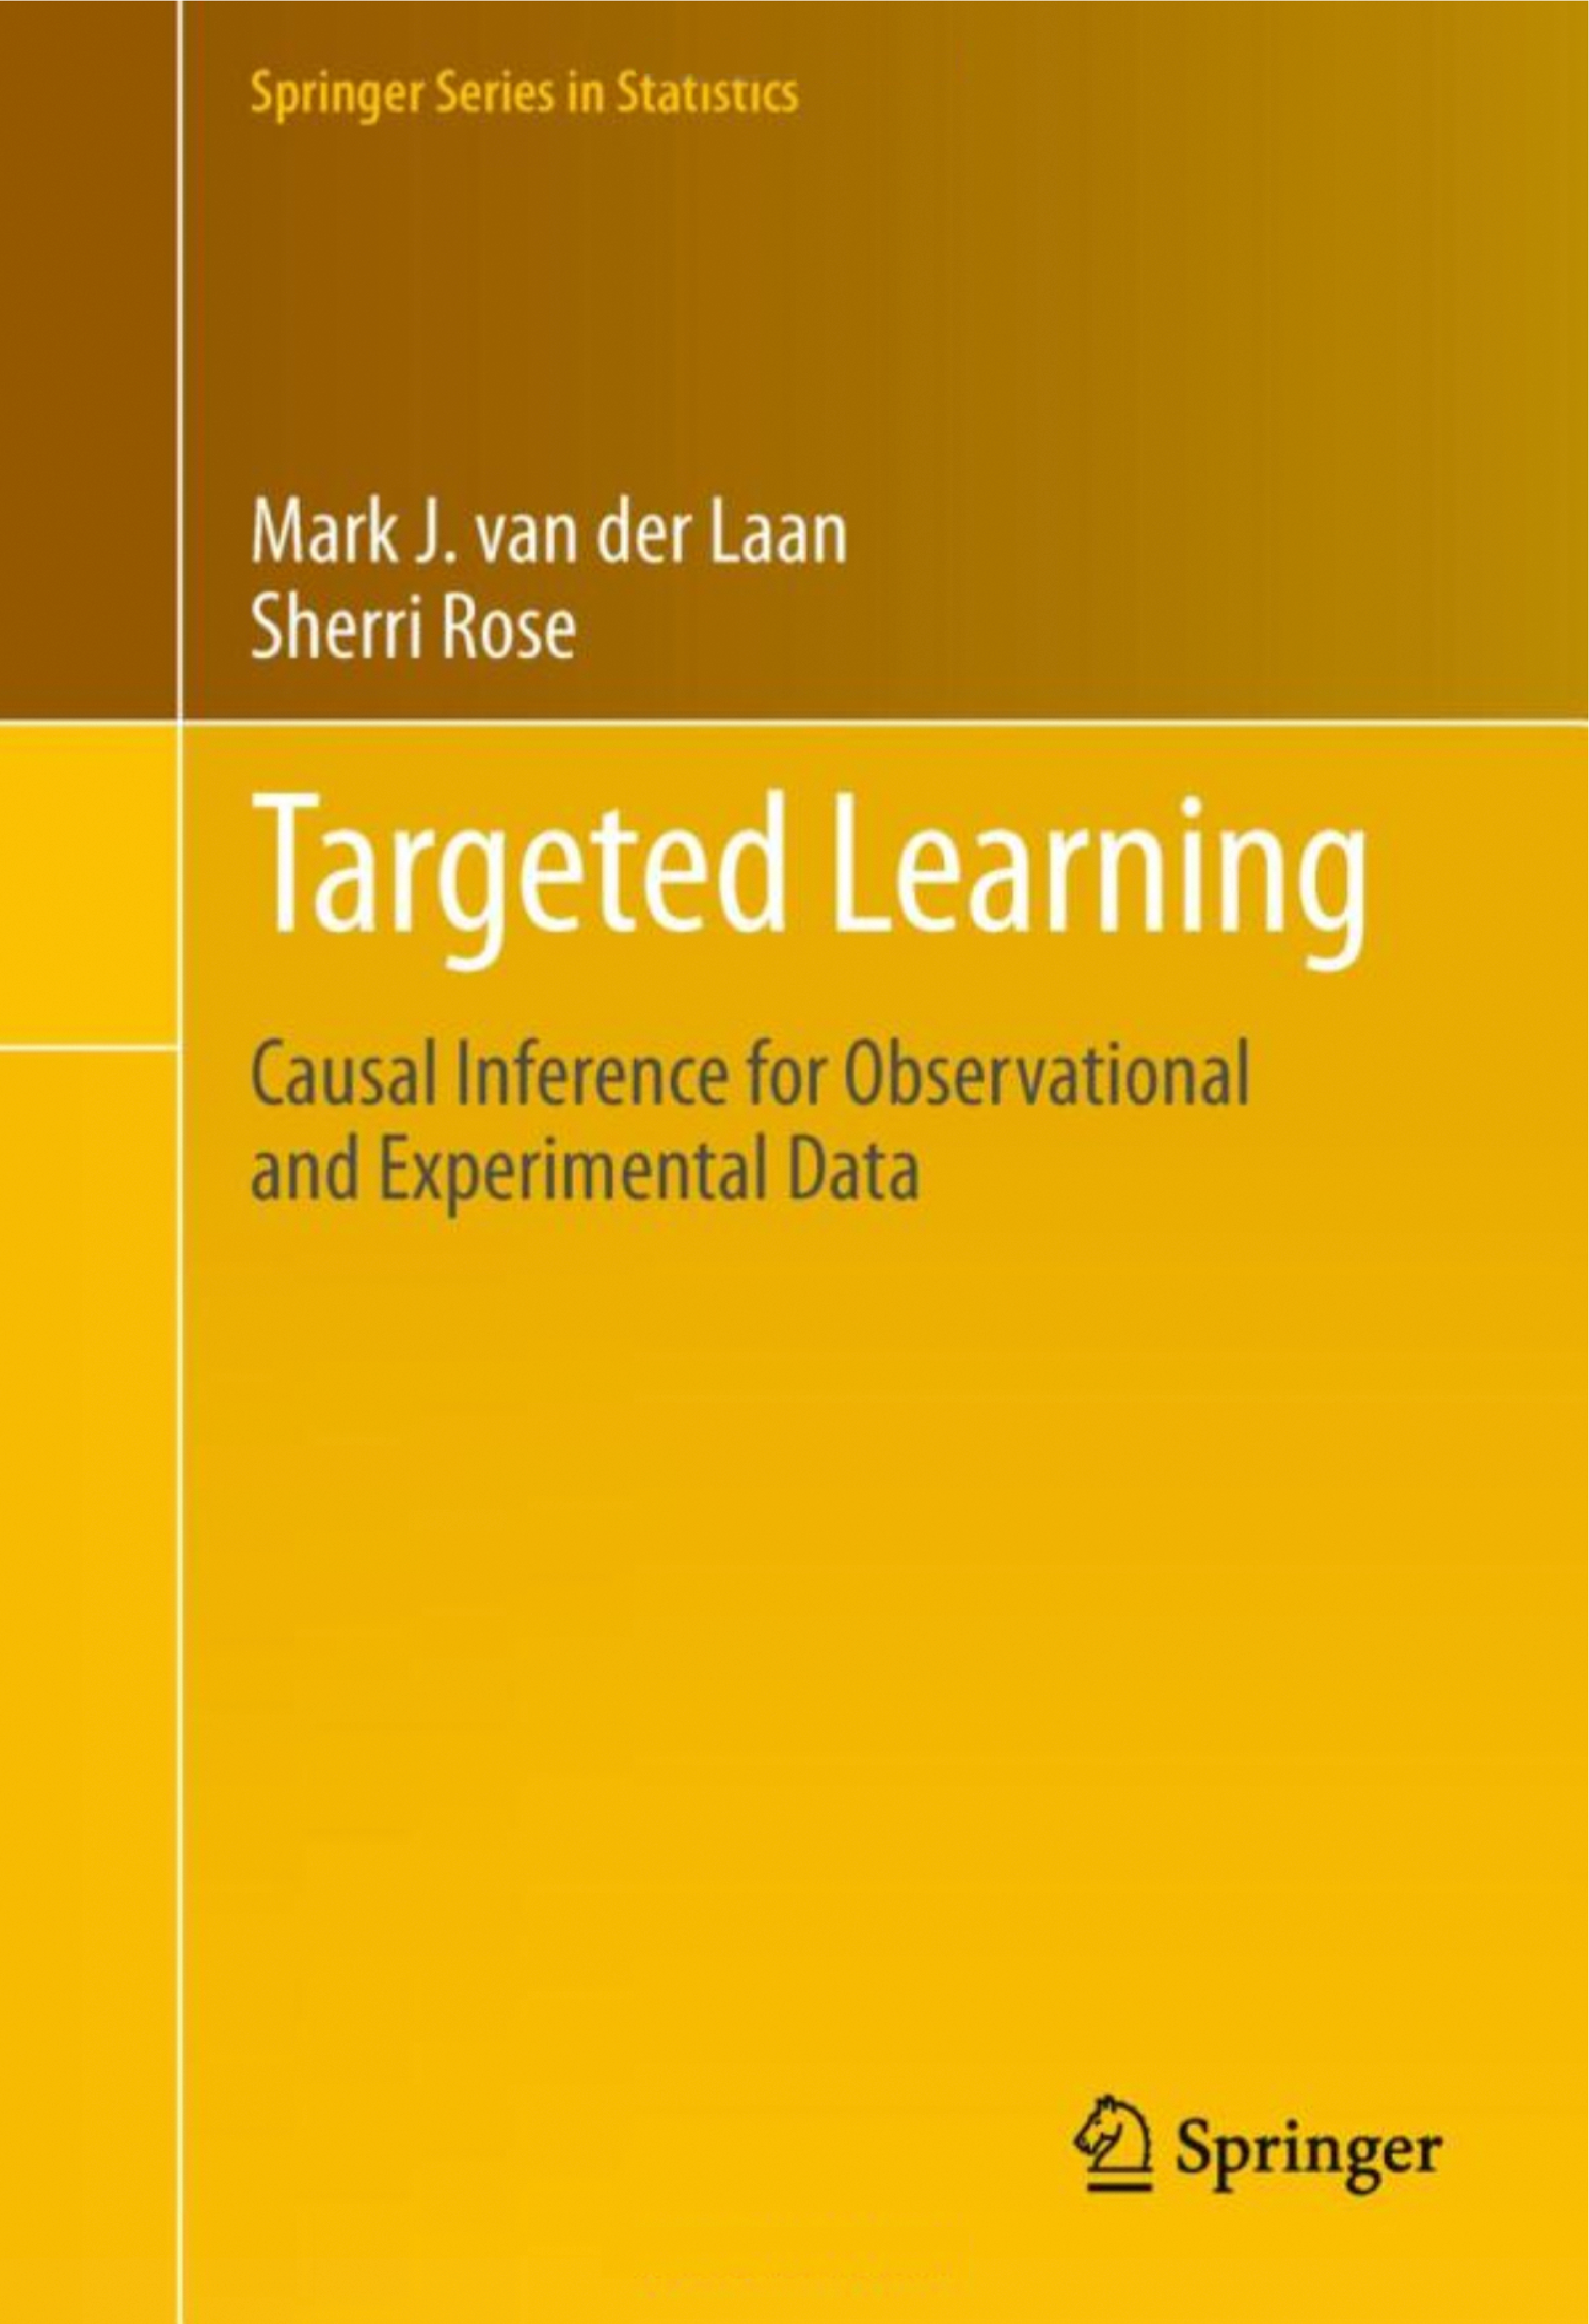
\includegraphics[height=1.7in]{figures/2011Book.pdf}}
\end{figure}
\end{center}
\end{column}
\begin{column}{4.9cm}
\begin{figure}
\fbox{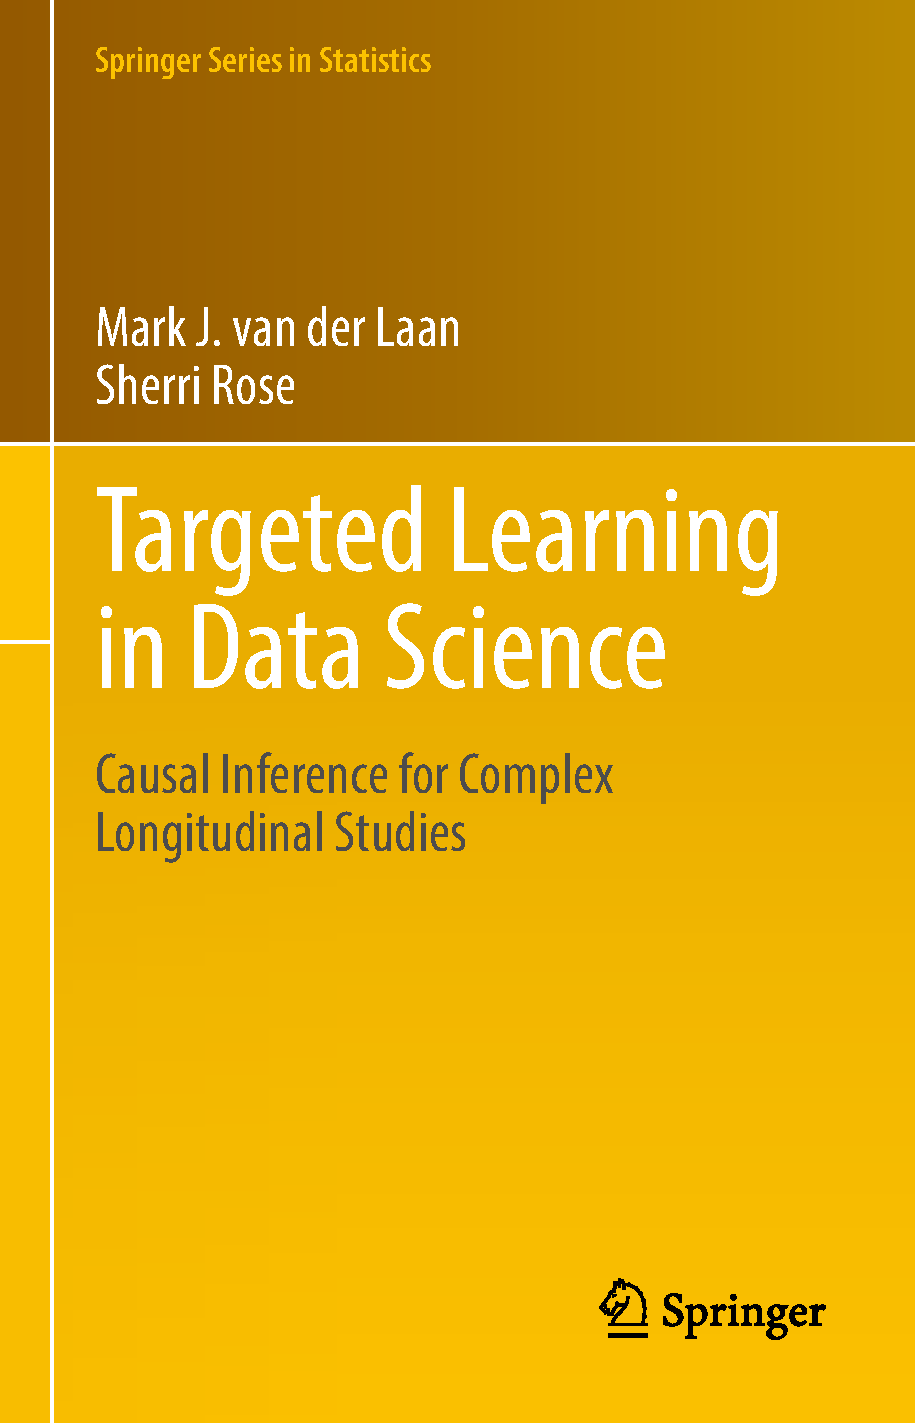
\includegraphics[height=1.7in]{figures/2018Book.pdf}}
\end{figure}
\end{column}
\end{columns}
\vspace{-10pt}
\begin{columns}
\begin{column}{4.9cm}
\begin{center}
{\footnotesize van der Laan \& Rose, \textit{Targeted Learning: Causal Inference for Observational and Experimental Data}. New York: Springer, 2011.}
\end{center}
\end{column}
\begin{column}{4.9cm}
\begin{center}
{\footnotesize van der Laan \& Rose, \textit{Targeted Learning in Data Science: Causal Inference for Complex Longitudinal Studies}. New York: Springer, 2018.}
\end{center}
\end{column}
\end{columns}
\vspace{15pt}
\centering
% \href{https://vanderlaan-lab.org}{https://vanderlaan-lab.org} \hspace{10mm}
  \href{https://tlverse.org/tlverse-handbook/}{Targeted Learning in \texttt{R}
  with the \texttt{tlverse}}
\end{frame}

\begin{frame}
\frametitle{Some applications of TL in the real world}
\vspace{-20pt}
\centering
\begin{figure}

\includegraphics[width = 1.05\textwidth]{figures/applications.pdf}
\end{figure}
\end{frame}

\begin{frame}
\frametitle{Better clinical decisions from observational data}
\vspace{-20pt}
\begin{center}
  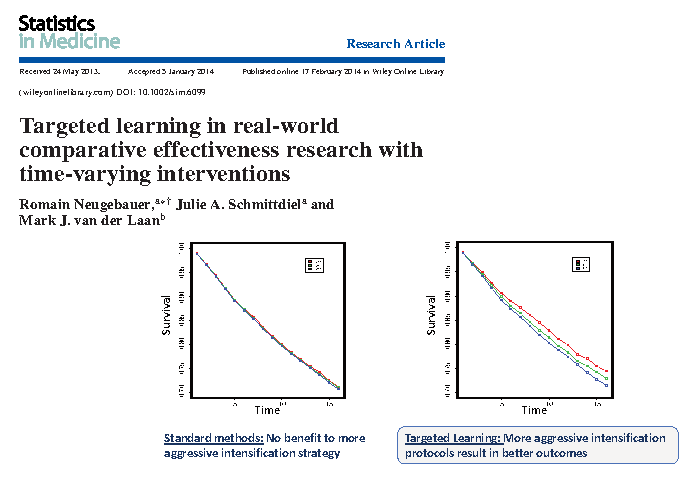
\includegraphics[width = 1.02\textwidth]{figures/diabetes.pdf}
  \end{center}
\end{frame}

% add applications of shift and optimal treatment
\begin{frame}
  \frametitle{TL for optimal treatment variable importance in meta-analysis of
  childhood development studies}
  \vspace{-1em}
  \begin{center}
  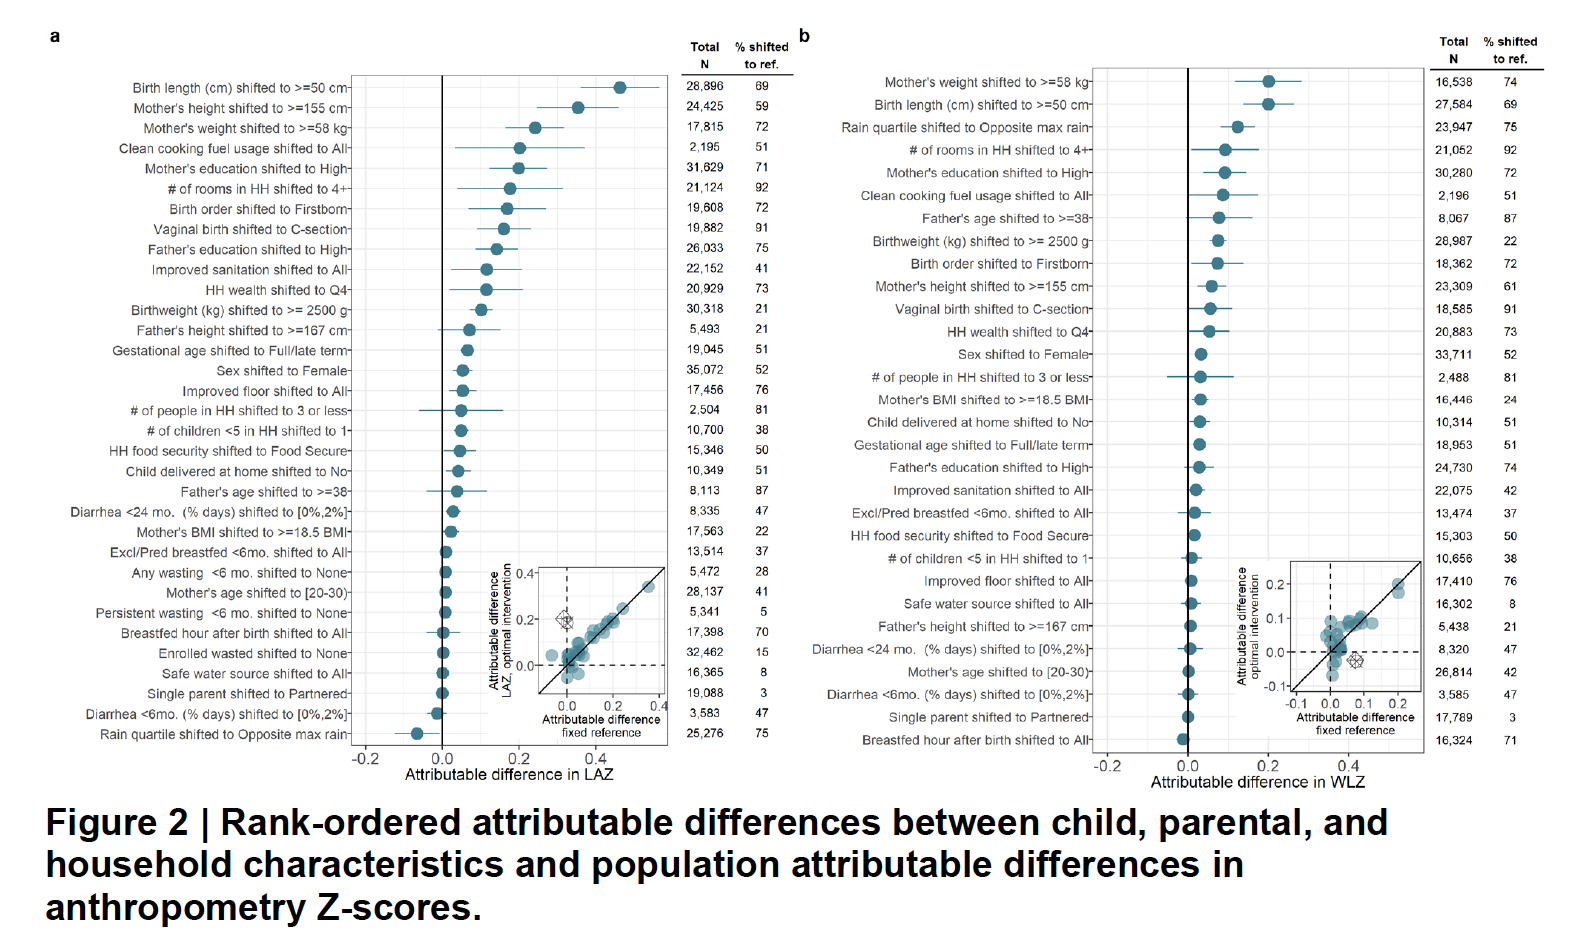
\includegraphics[width=1.03\textwidth] {figures/NatureChildDevCons,png}\hspace*{6cm}
  \end{center}
\end{frame}

\begin{frame}
  \frametitle{Evaluating counterfactual HIV infection risk after shifting
  vaccine-induced immune response markers}
  \vspace{-2em}
  \begin{center}
  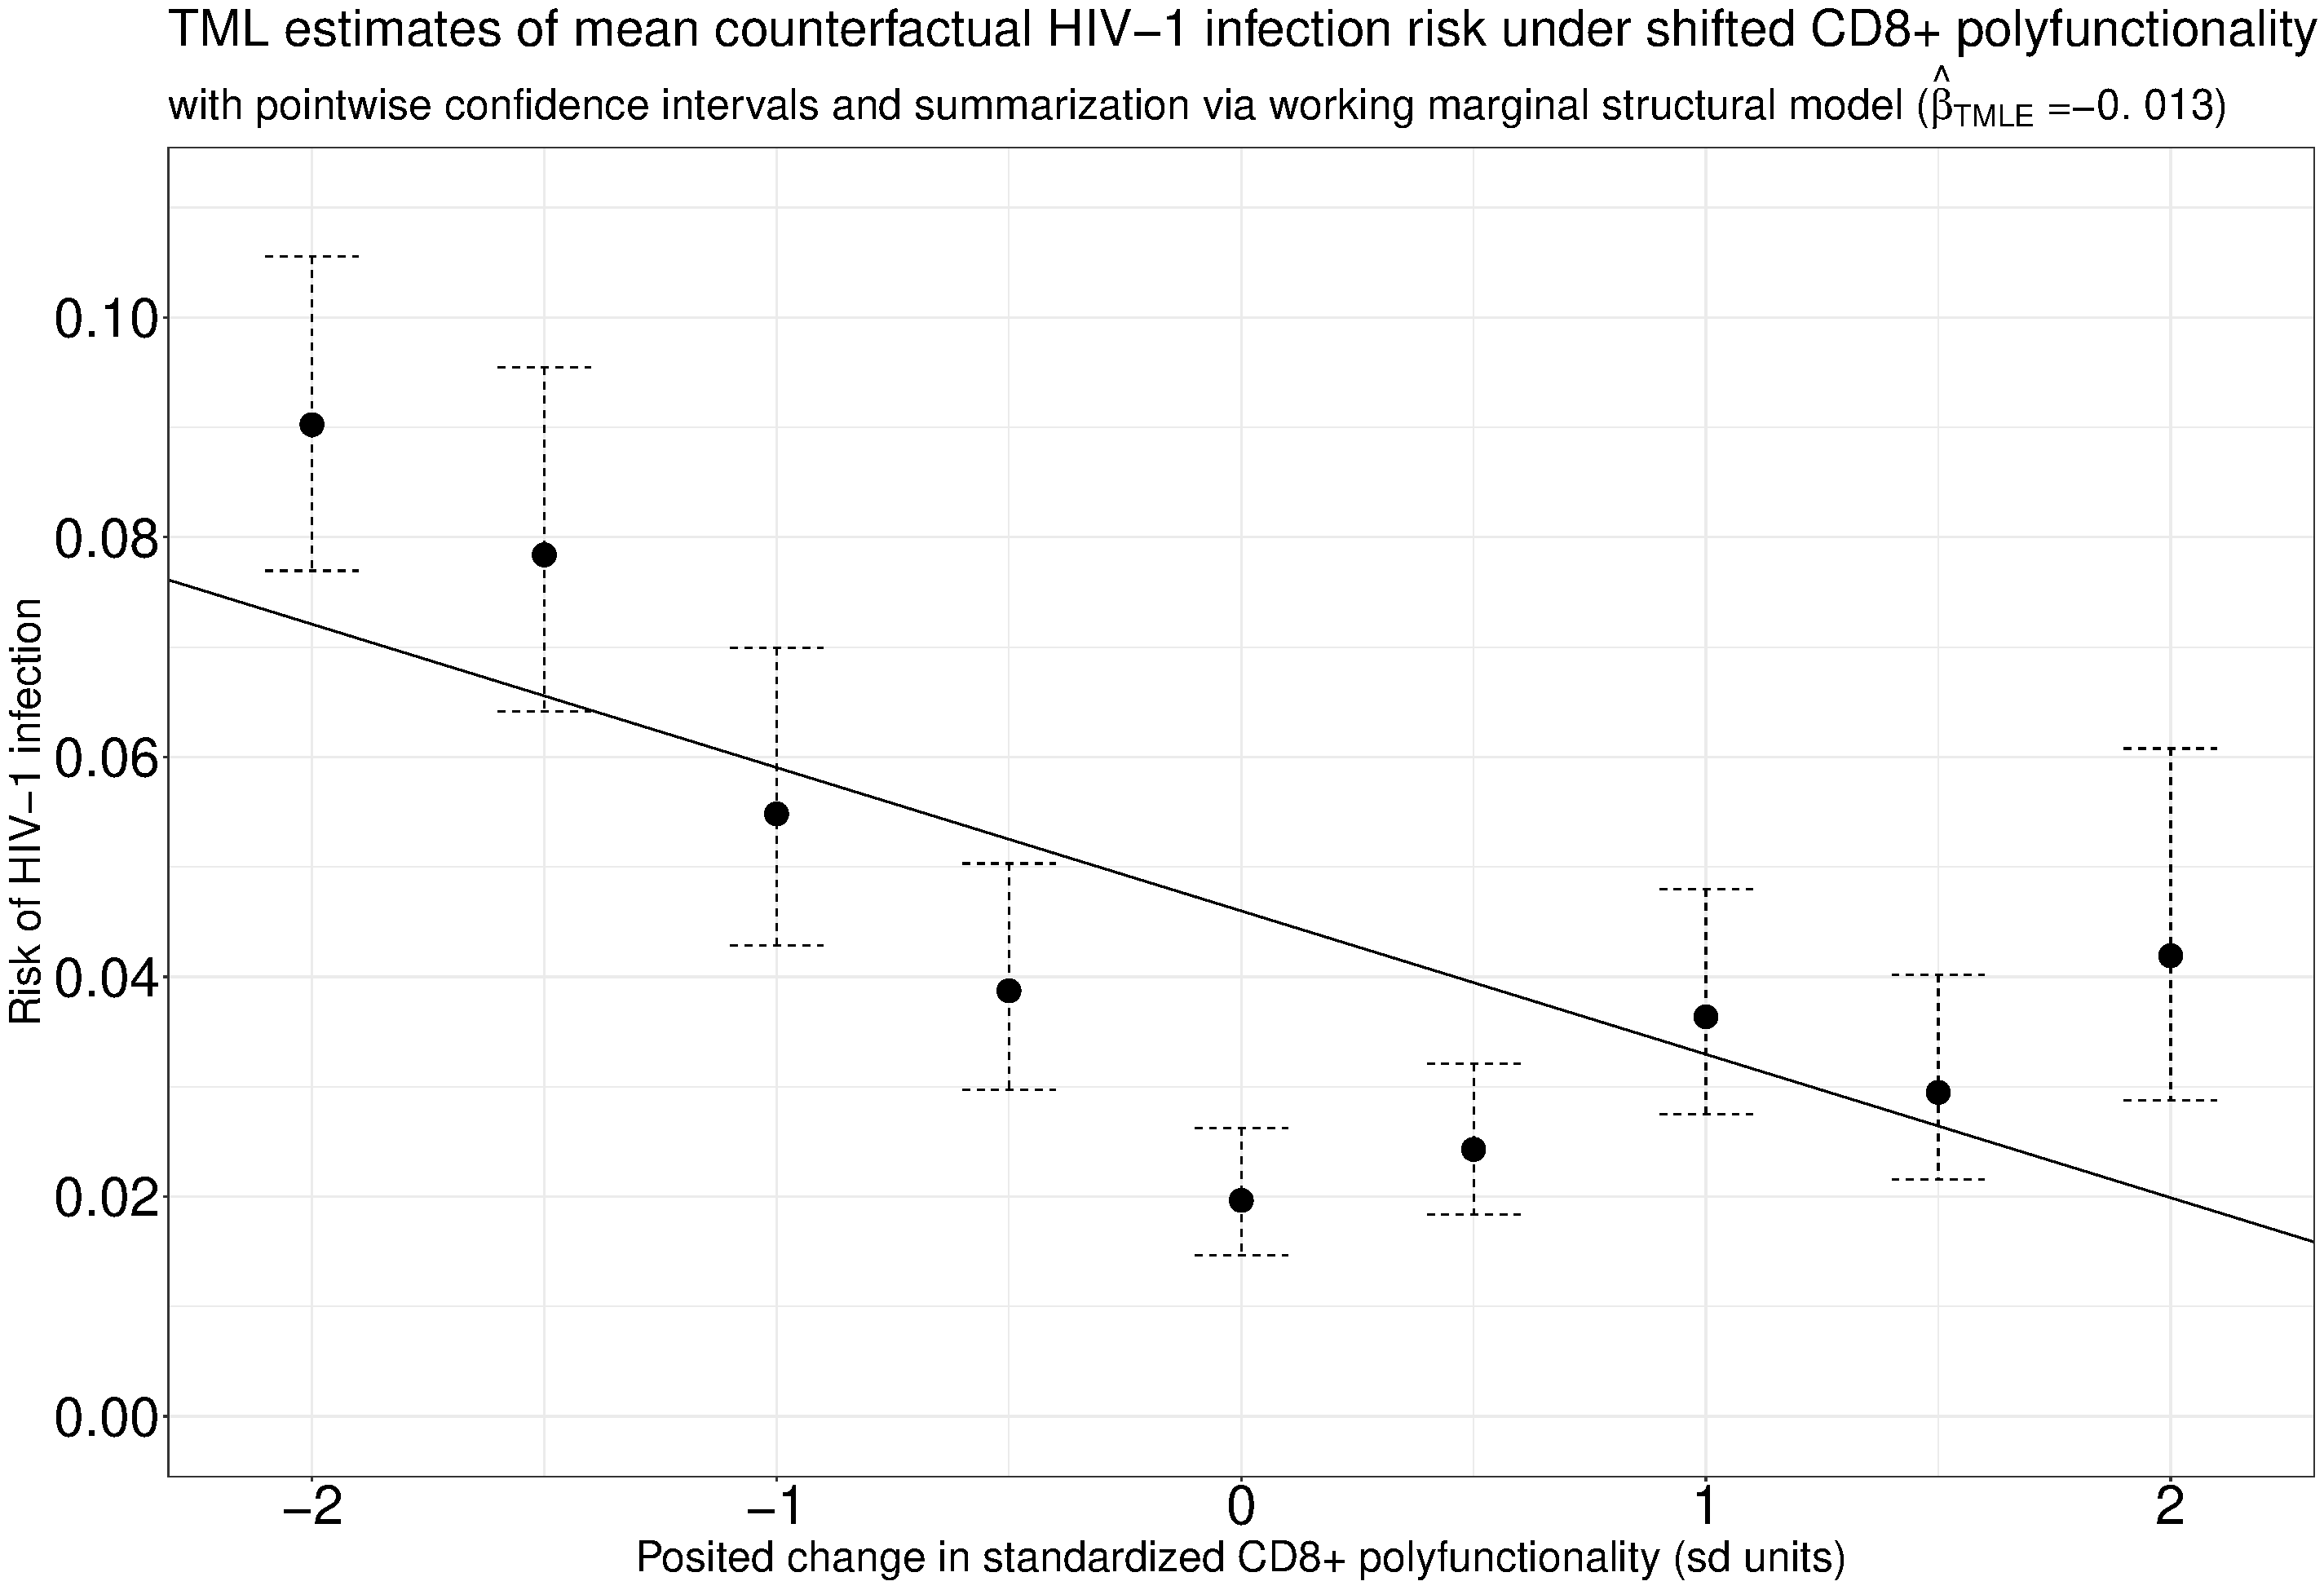
\includegraphics[width=0.93\textwidth] {figures/HejaziShiftCD8_2021.pdf}\hspace*{4cm}
  \end{center}
  \scriptsize{
  Hejazi et al.~``Efficient nonparametric inference on the effects of stochastic
  interventions under two-phase sampling, with applications to vaccine efficacy
  trials'' \textit{Biometrics} (2021).
  \href{https://doi.org/10.1111/biom.13375}{10.1111/biom.13375}}
\end{frame}

\begin{frame}
  \frametitle{Evaluating COVID-19 vaccine efficacy after shifting immune
  correlates of protection}
  \vspace{-2em}
  \begin{center}
  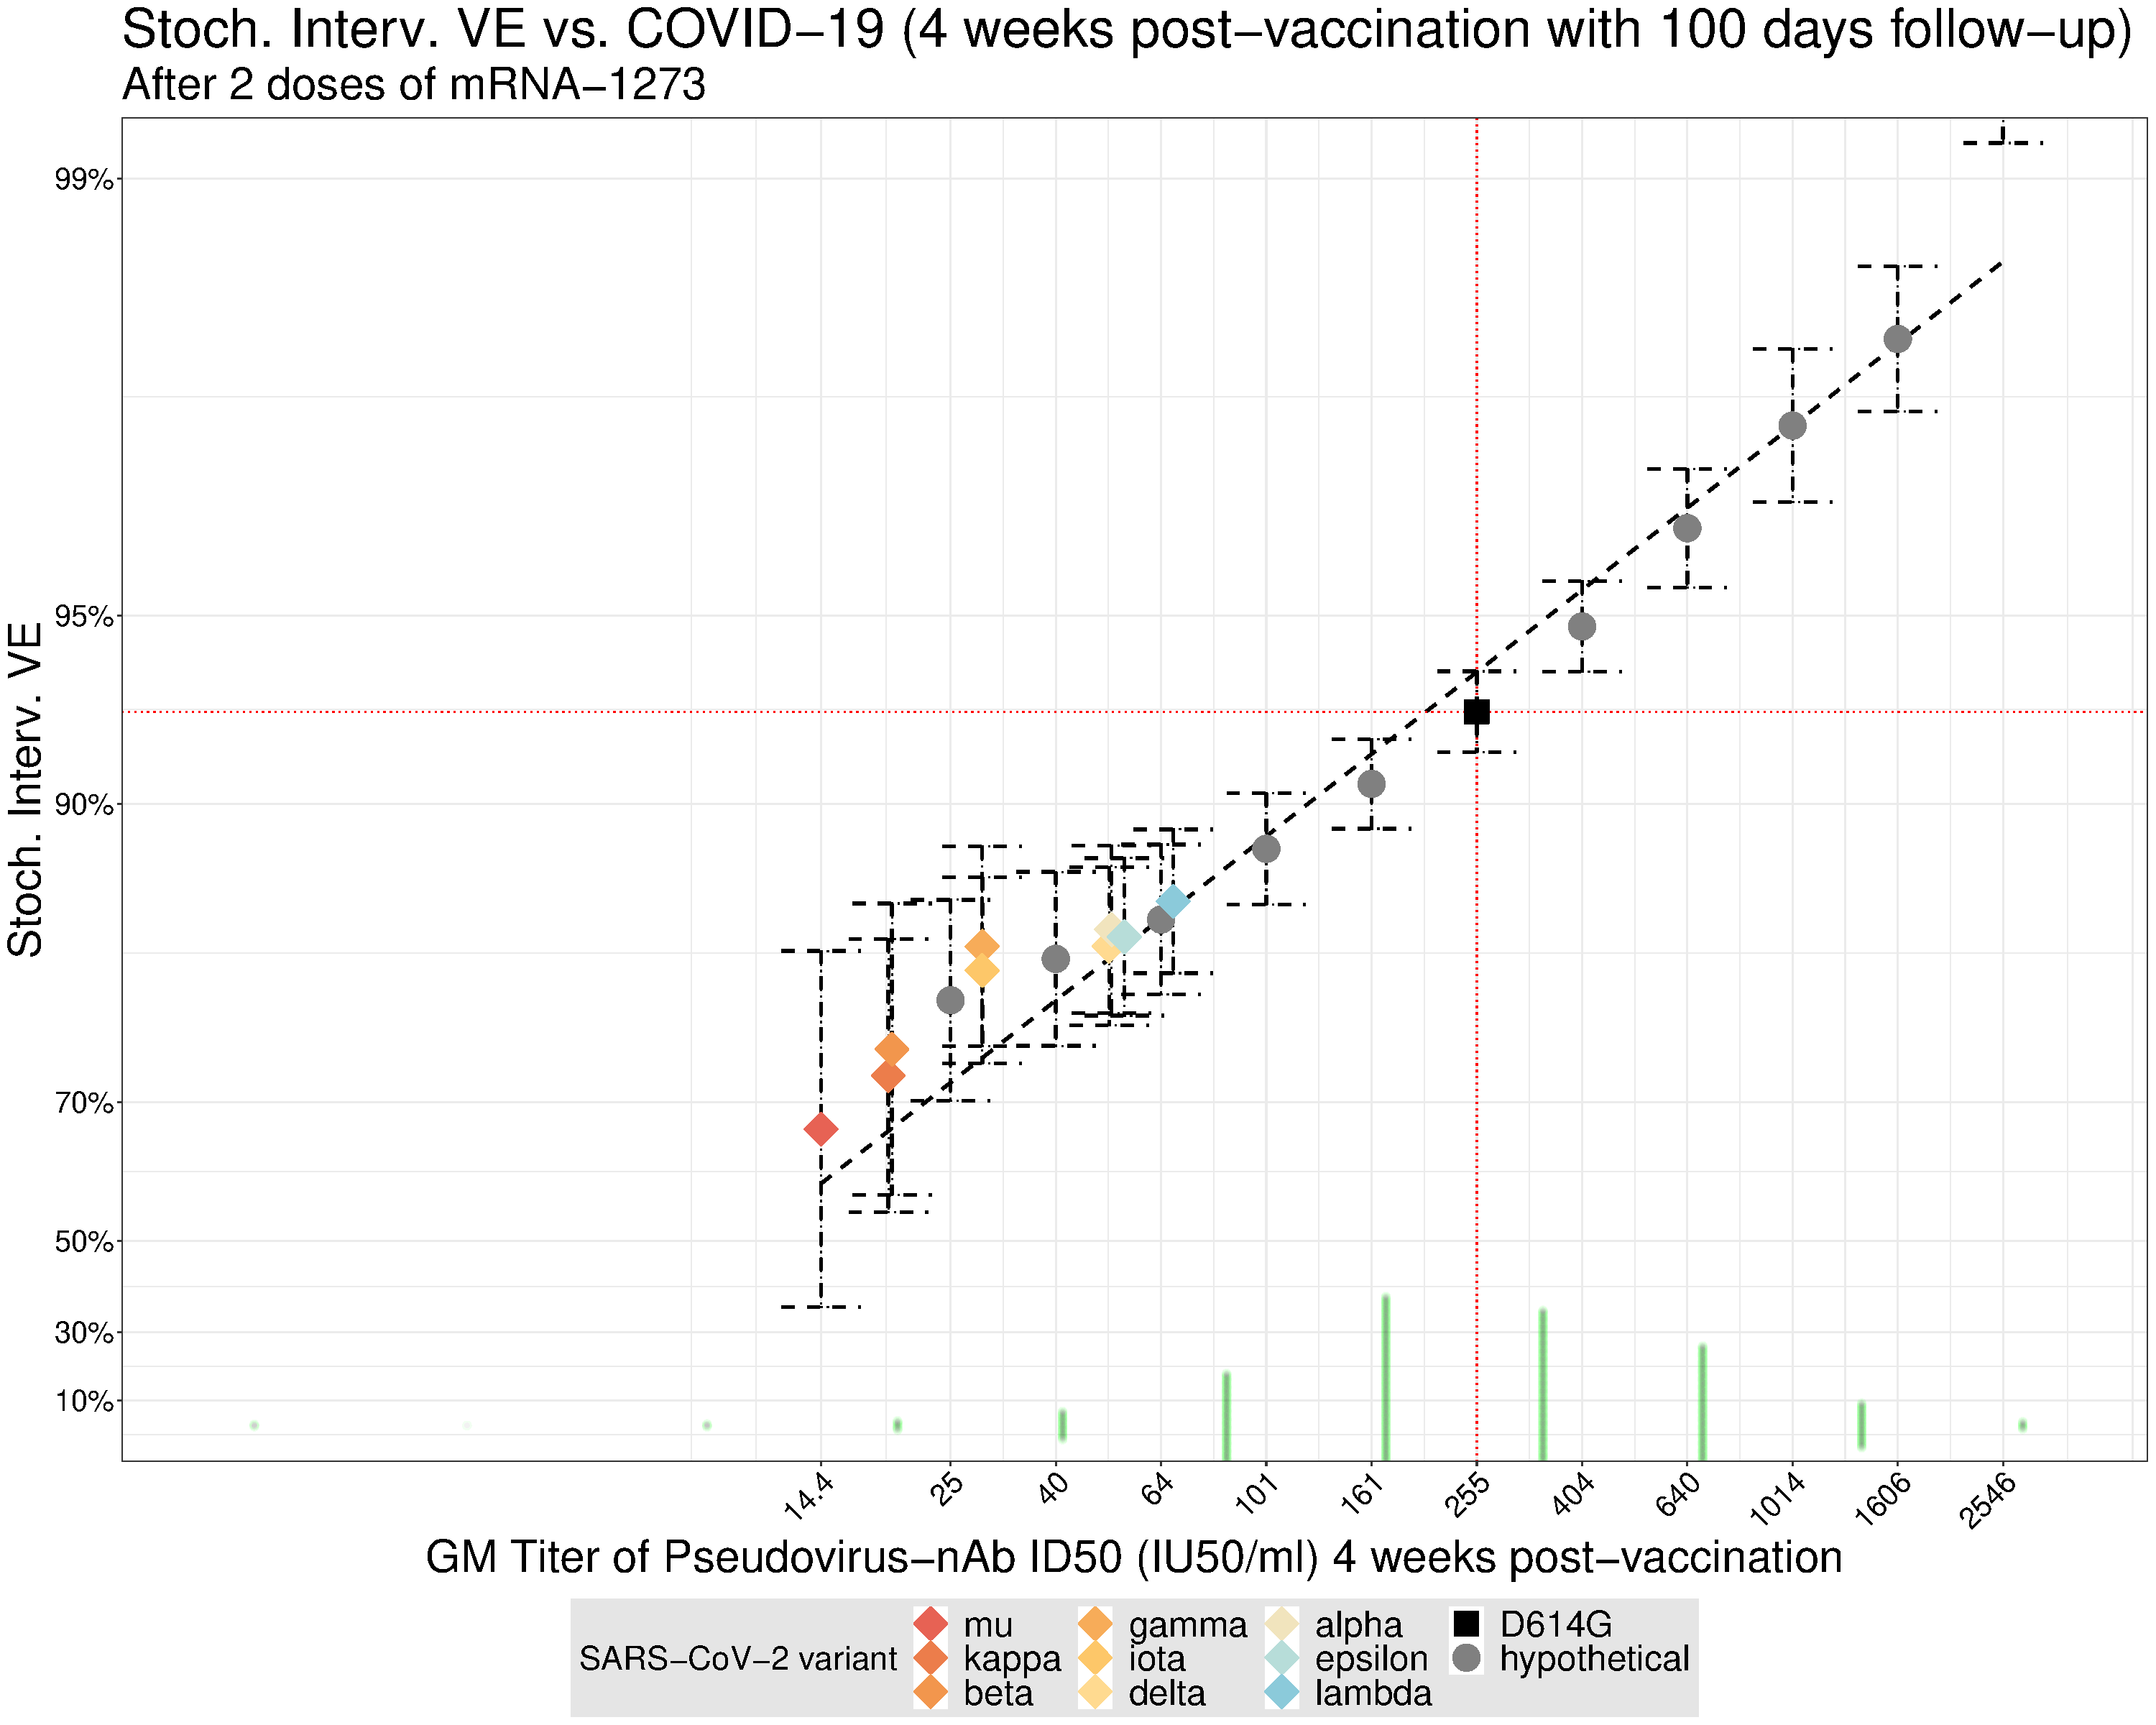
\includegraphics[width=0.85\textwidth]
  {figures/sve_pseudoneutid50_immunobridging_2dose.pdf}\hspace*{4cm}
  \end{center}
  \scriptsize{
  Hejazi et al.~``Stochastic interventional approach to assessing immune
  correlates of protection: Application to the COVE mRNA-1273 vaccine trial''
  \textit{IJID} (2023).}
  %\href{https://doi.org/10.1016/j.ijid.2023.09.012}{10.1016/j.ijid.2023.09.012}}
\end{frame}

\begin{frame}
  \frametitle{Evaluating (in)direct effects of adaptive dosing strategies for OUD}
  \vspace{-2em}
  \begin{center}
  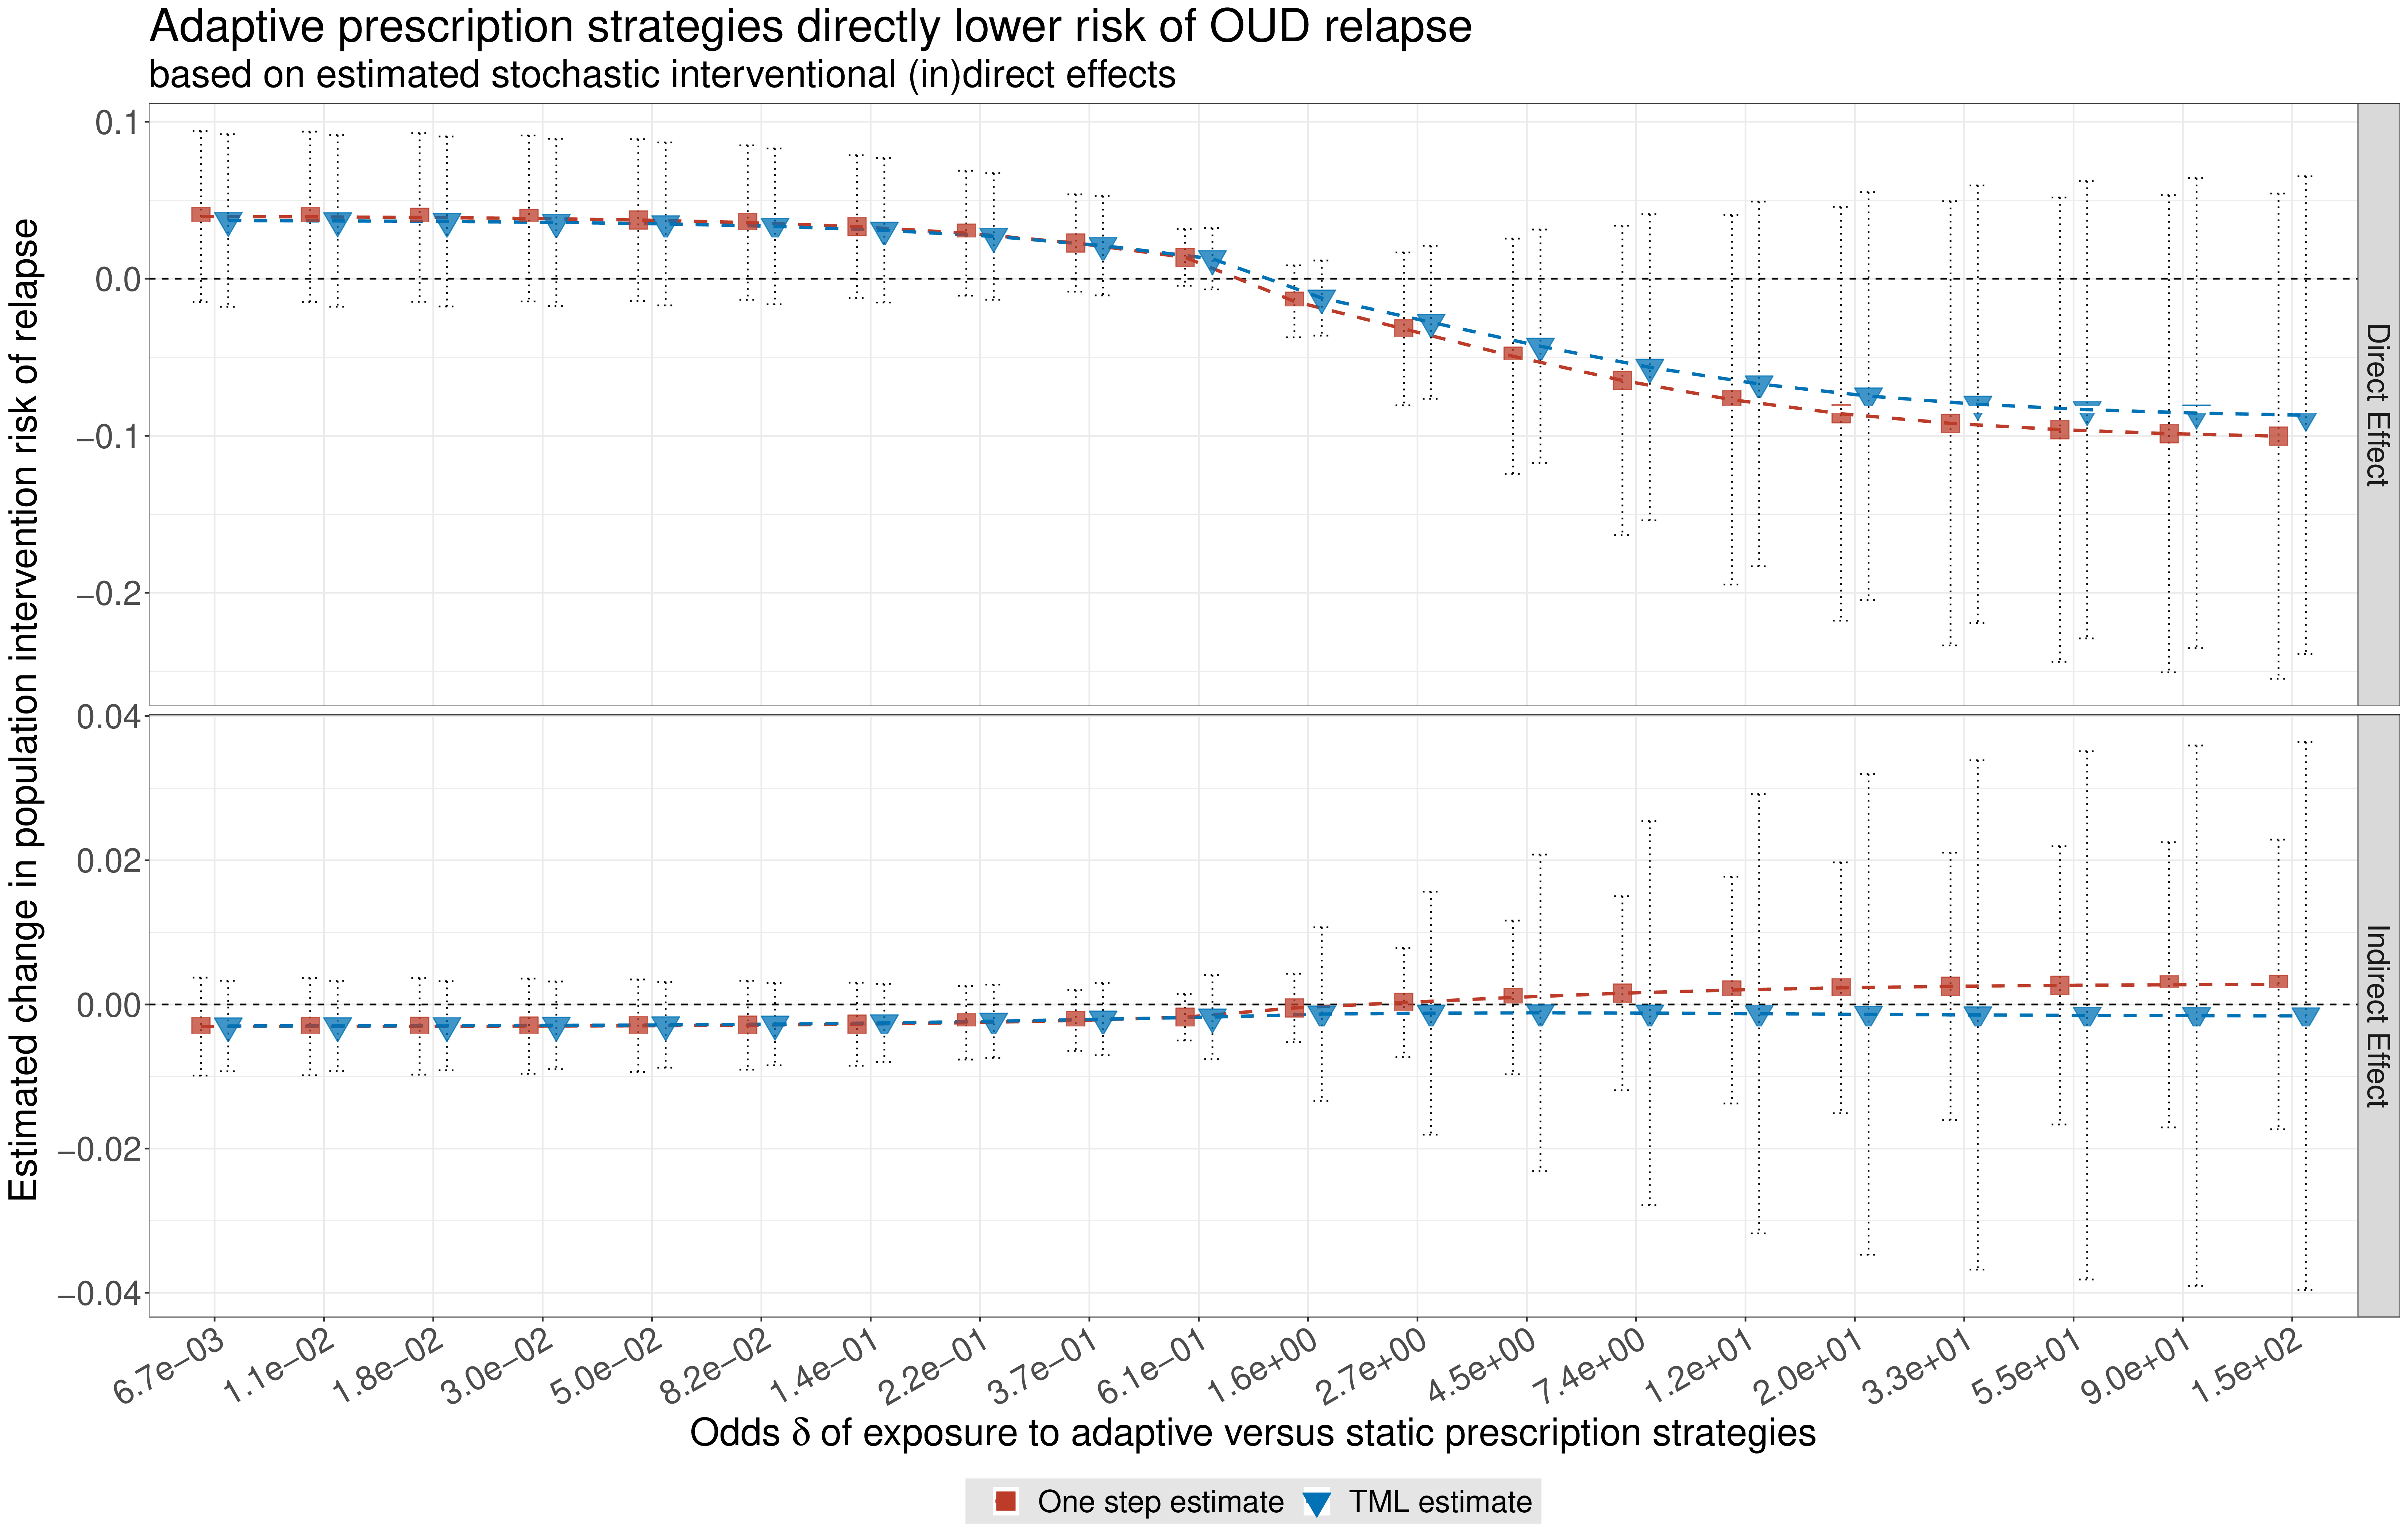
\includegraphics[width=0.96\textwidth] {figures/hejazi_xbot.png}\hspace*{4cm}
  \end{center}
  \scriptsize{
  Hejazi et al., ``Nonparametric causal mediation analysis for stochastic
  interventional (in)direct effects.'' \textit{Biostatistics} (2023).}
\end{frame}

\begin{frame}
  \frametitle{Estimating impacts on AKI of delay-in-intubation policies}
  \vspace{-2em}
  \begin{center}
  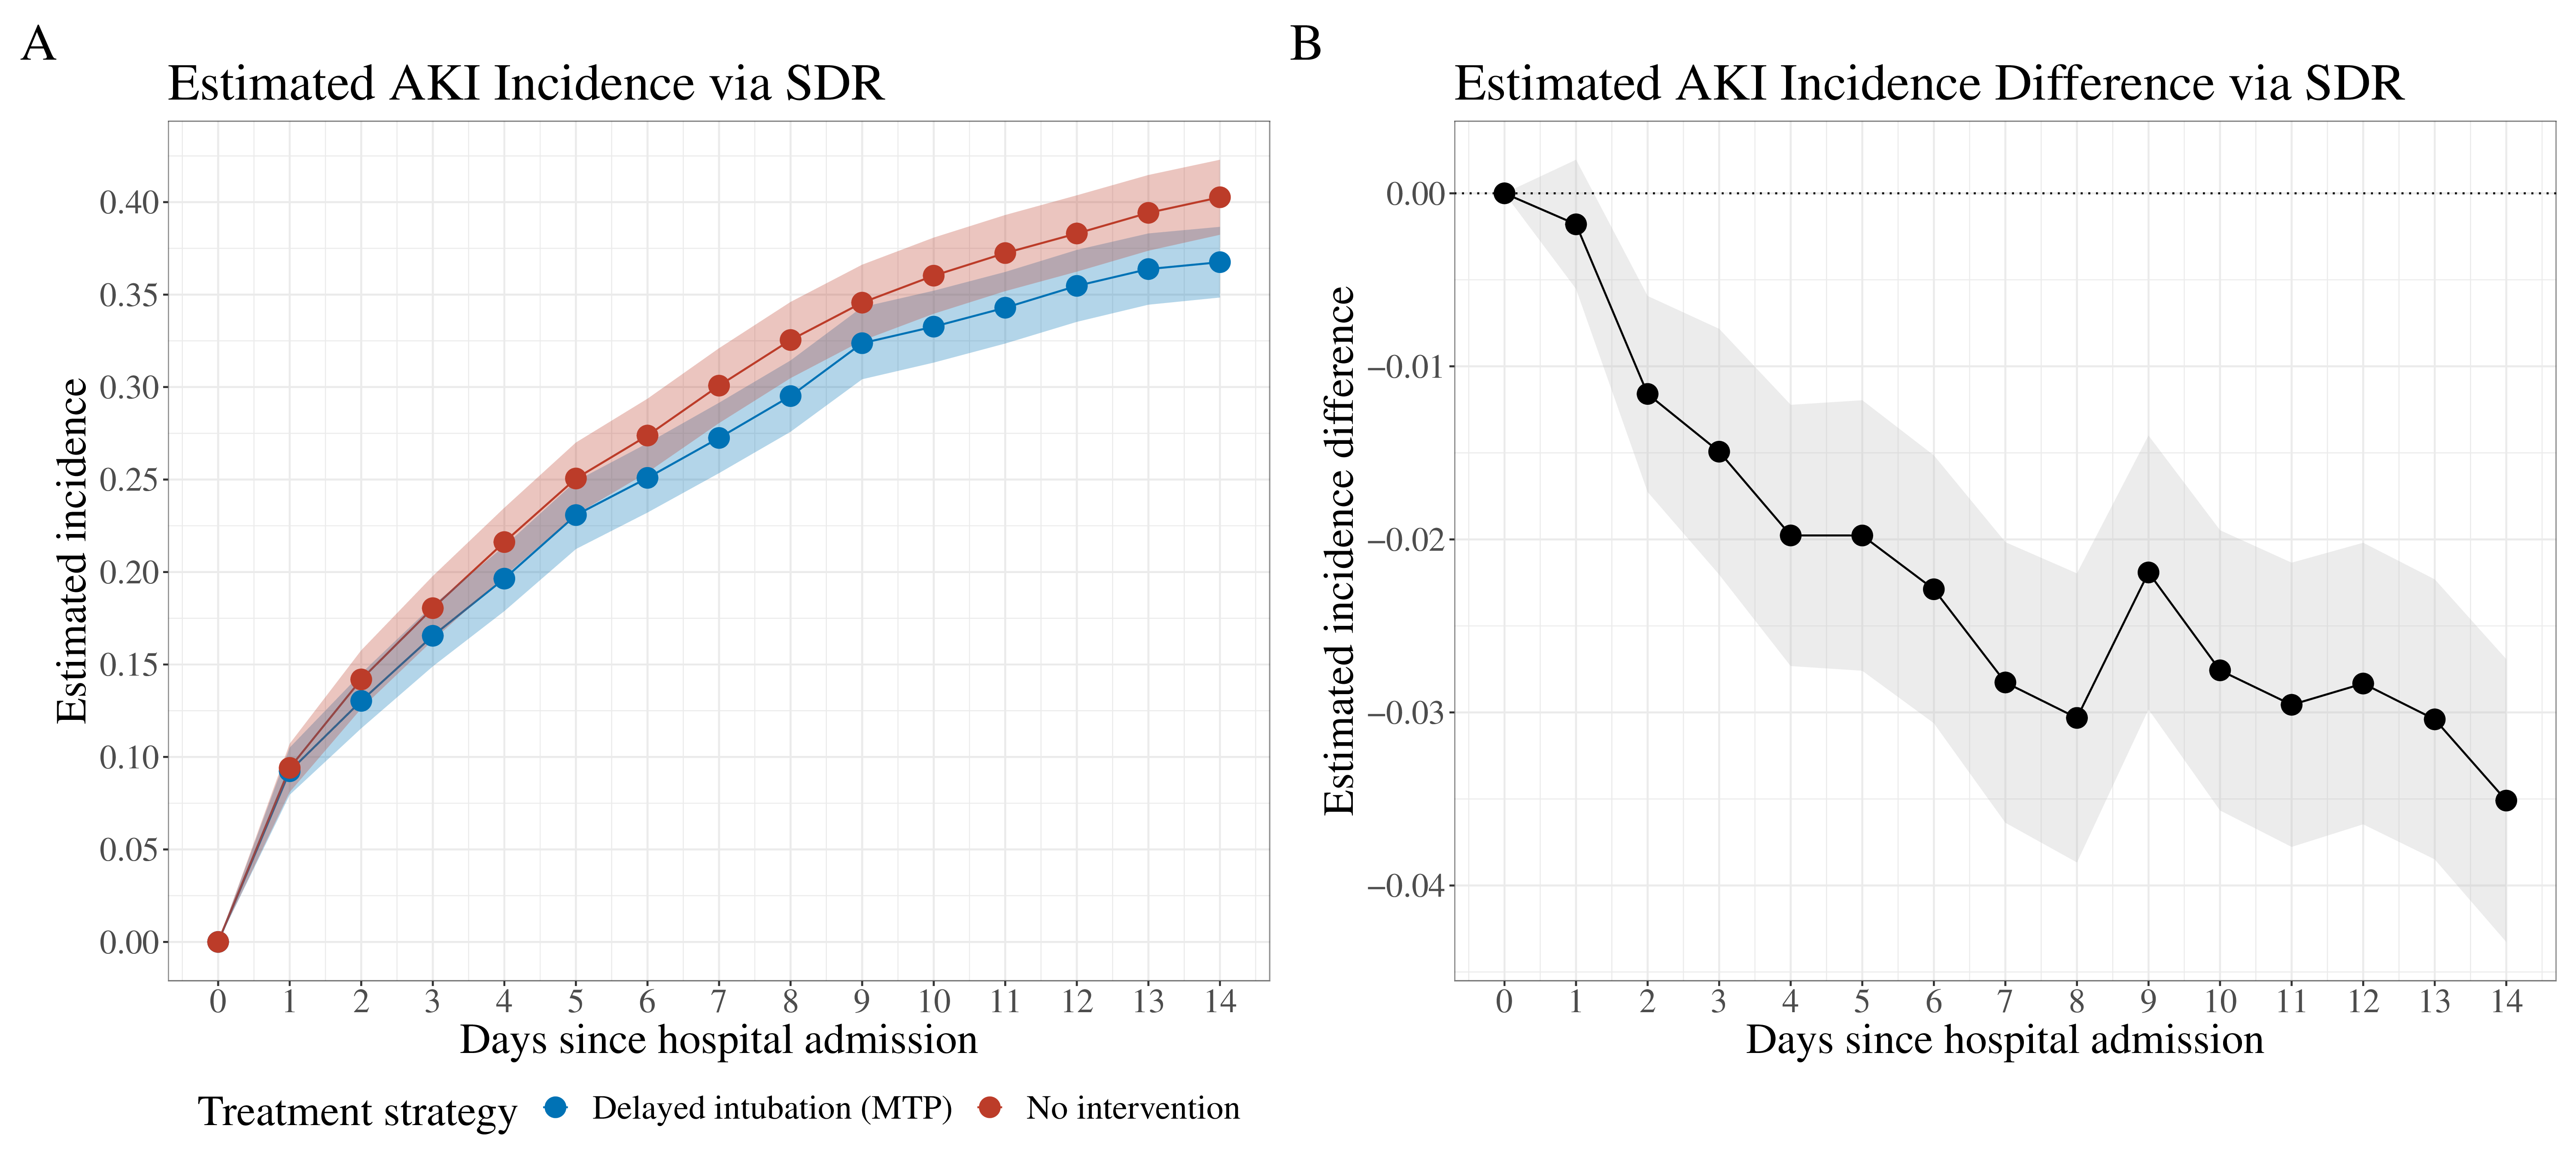
\includegraphics[width=1.03\textwidth] {figures/hejazi_surv_lmtp.png}\hspace*{4cm}
  \end{center}
  \scriptsize{
  Diaz, Hoffman, and Hejazi, ``Causal survival analysis with longitudinal
  modified treatment policies.'' \textit{LiDA} (2024).}
\end{frame}

% \begin{frame}
%   \frametitle{Estimating impacts on COVID-19 infection rates by longitudinal
%   policy shift interventions}
%   \vspace{-2em}
%   \begin{center}
%   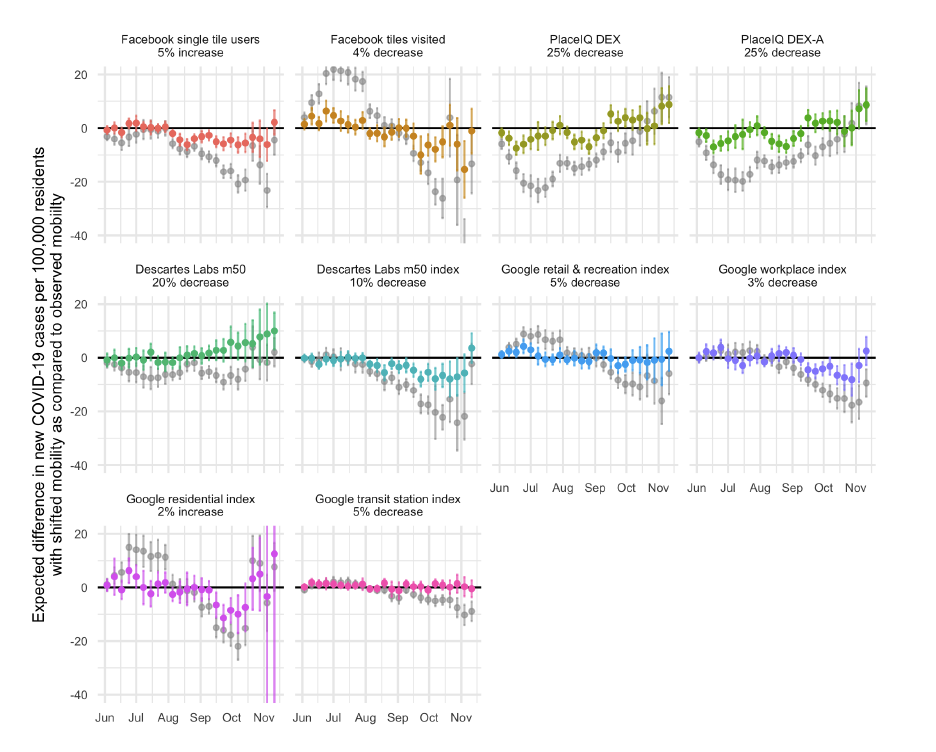
\includegraphics[width=0.8\textwidth] {figures/BalzerShift2023.png}\hspace*{4cm}
%   \end{center}
%   \scriptsize{
%   Nugent and Balzer, ``A demonstration of modified treatment policies to
%   evaluate shifts in mobility and COVID-19 case rates in US counties.''
%   \textit{AJE} (2023).}
% \end{frame}

\begin{frame}
  \frametitle{Introduction to the \texttt{tlverse}}
  \url{https://tlverse.org/catalyst2024-workshop/}
\end{frame}

\section{TL Roadmap}

\begin{frame}
  \frametitle{A roadmap for learning from data}
  \vspace{-20pt}
  \begin{center}
  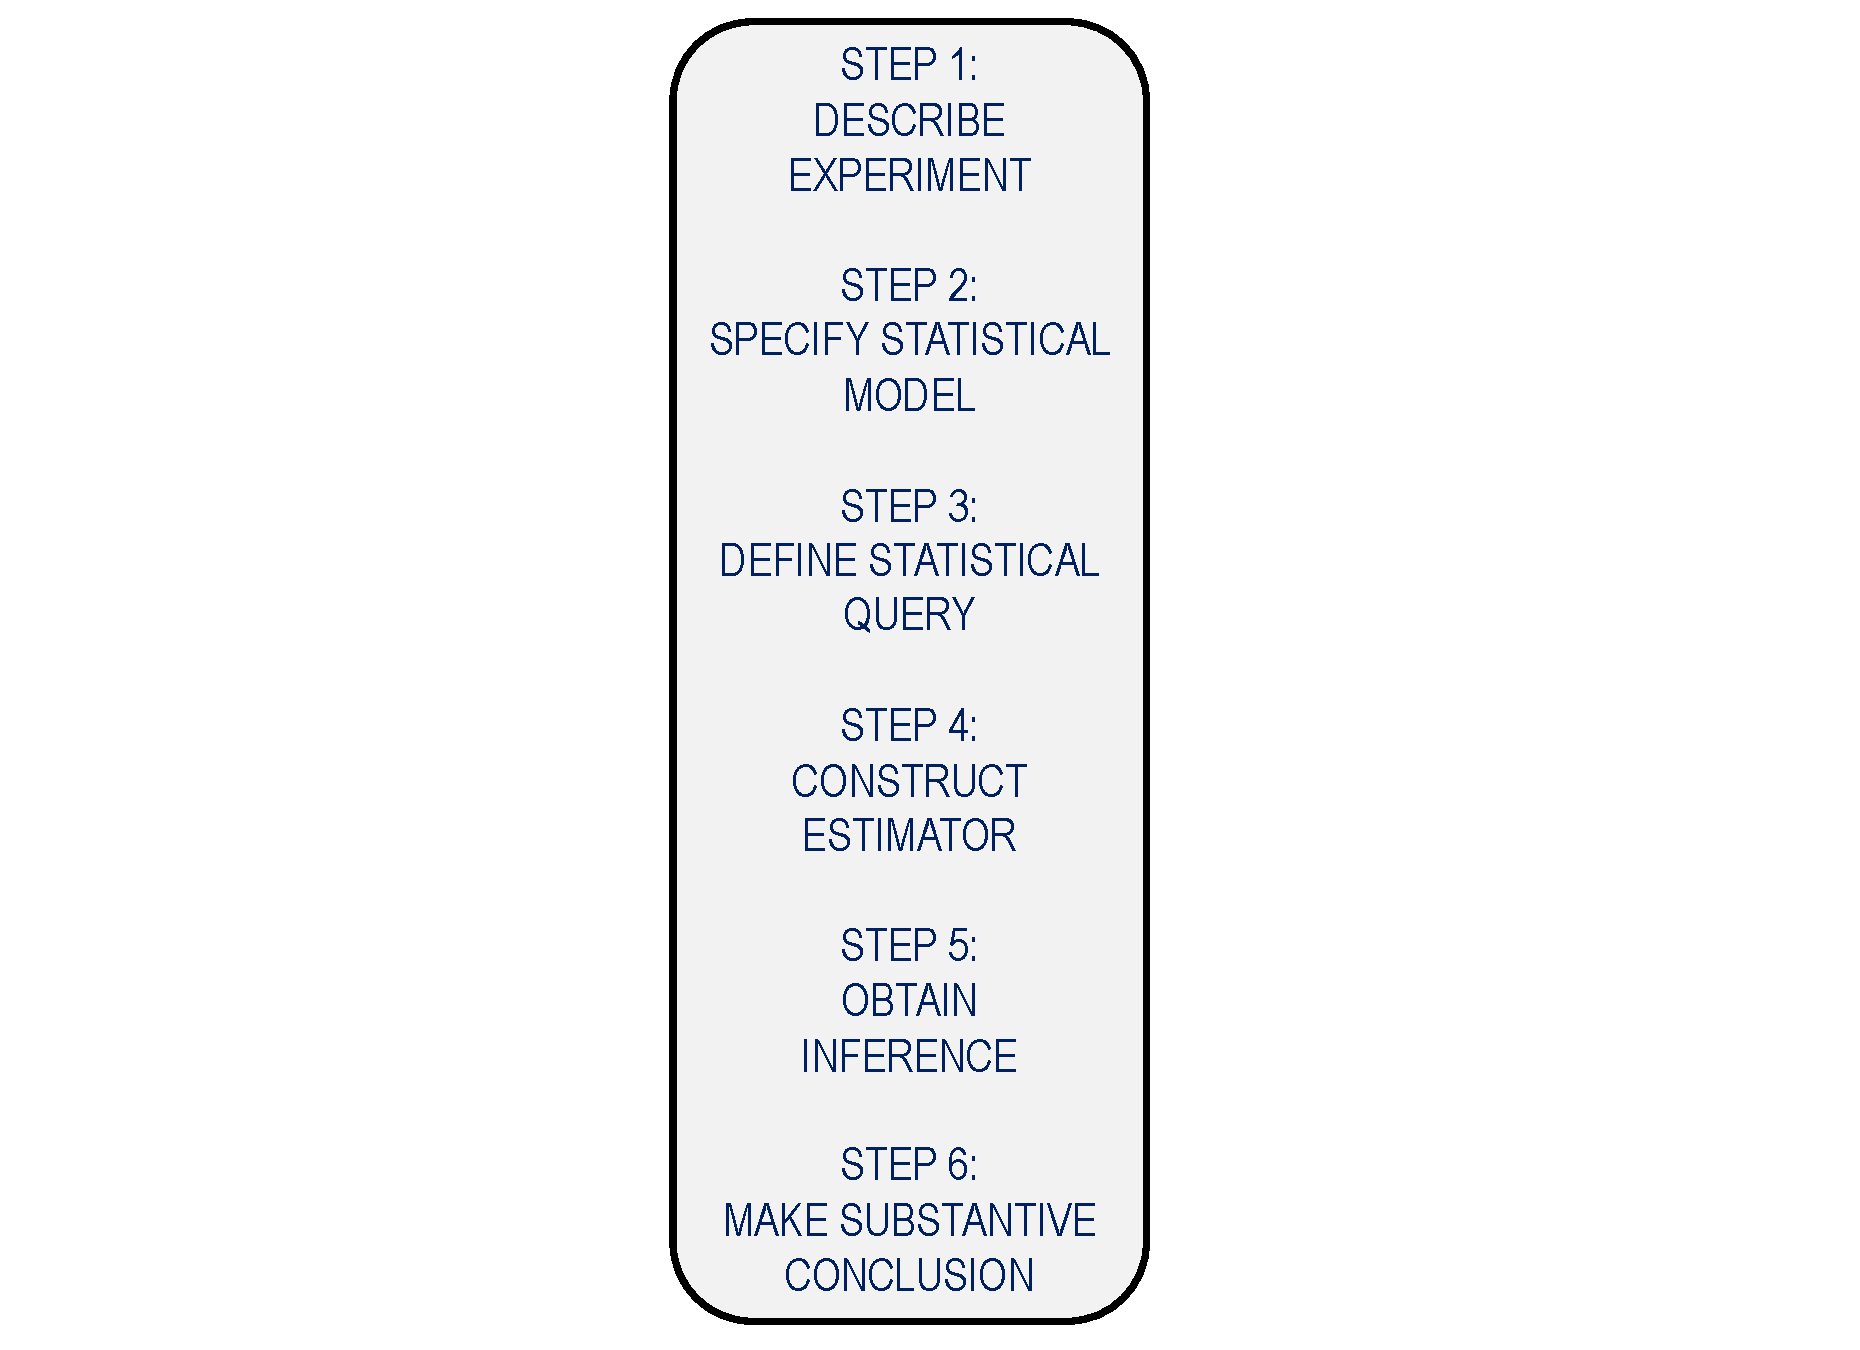
\includegraphics[width = 1.05\textwidth]{figures/roadmap.pdf}
  \end{center}
\end{frame}

\subsection{Describe study}
\begin{frame}
  \frametitle{Step 1: What is the data-generating experiment?}
  \vspace{-20pt}
  \begin{center}
  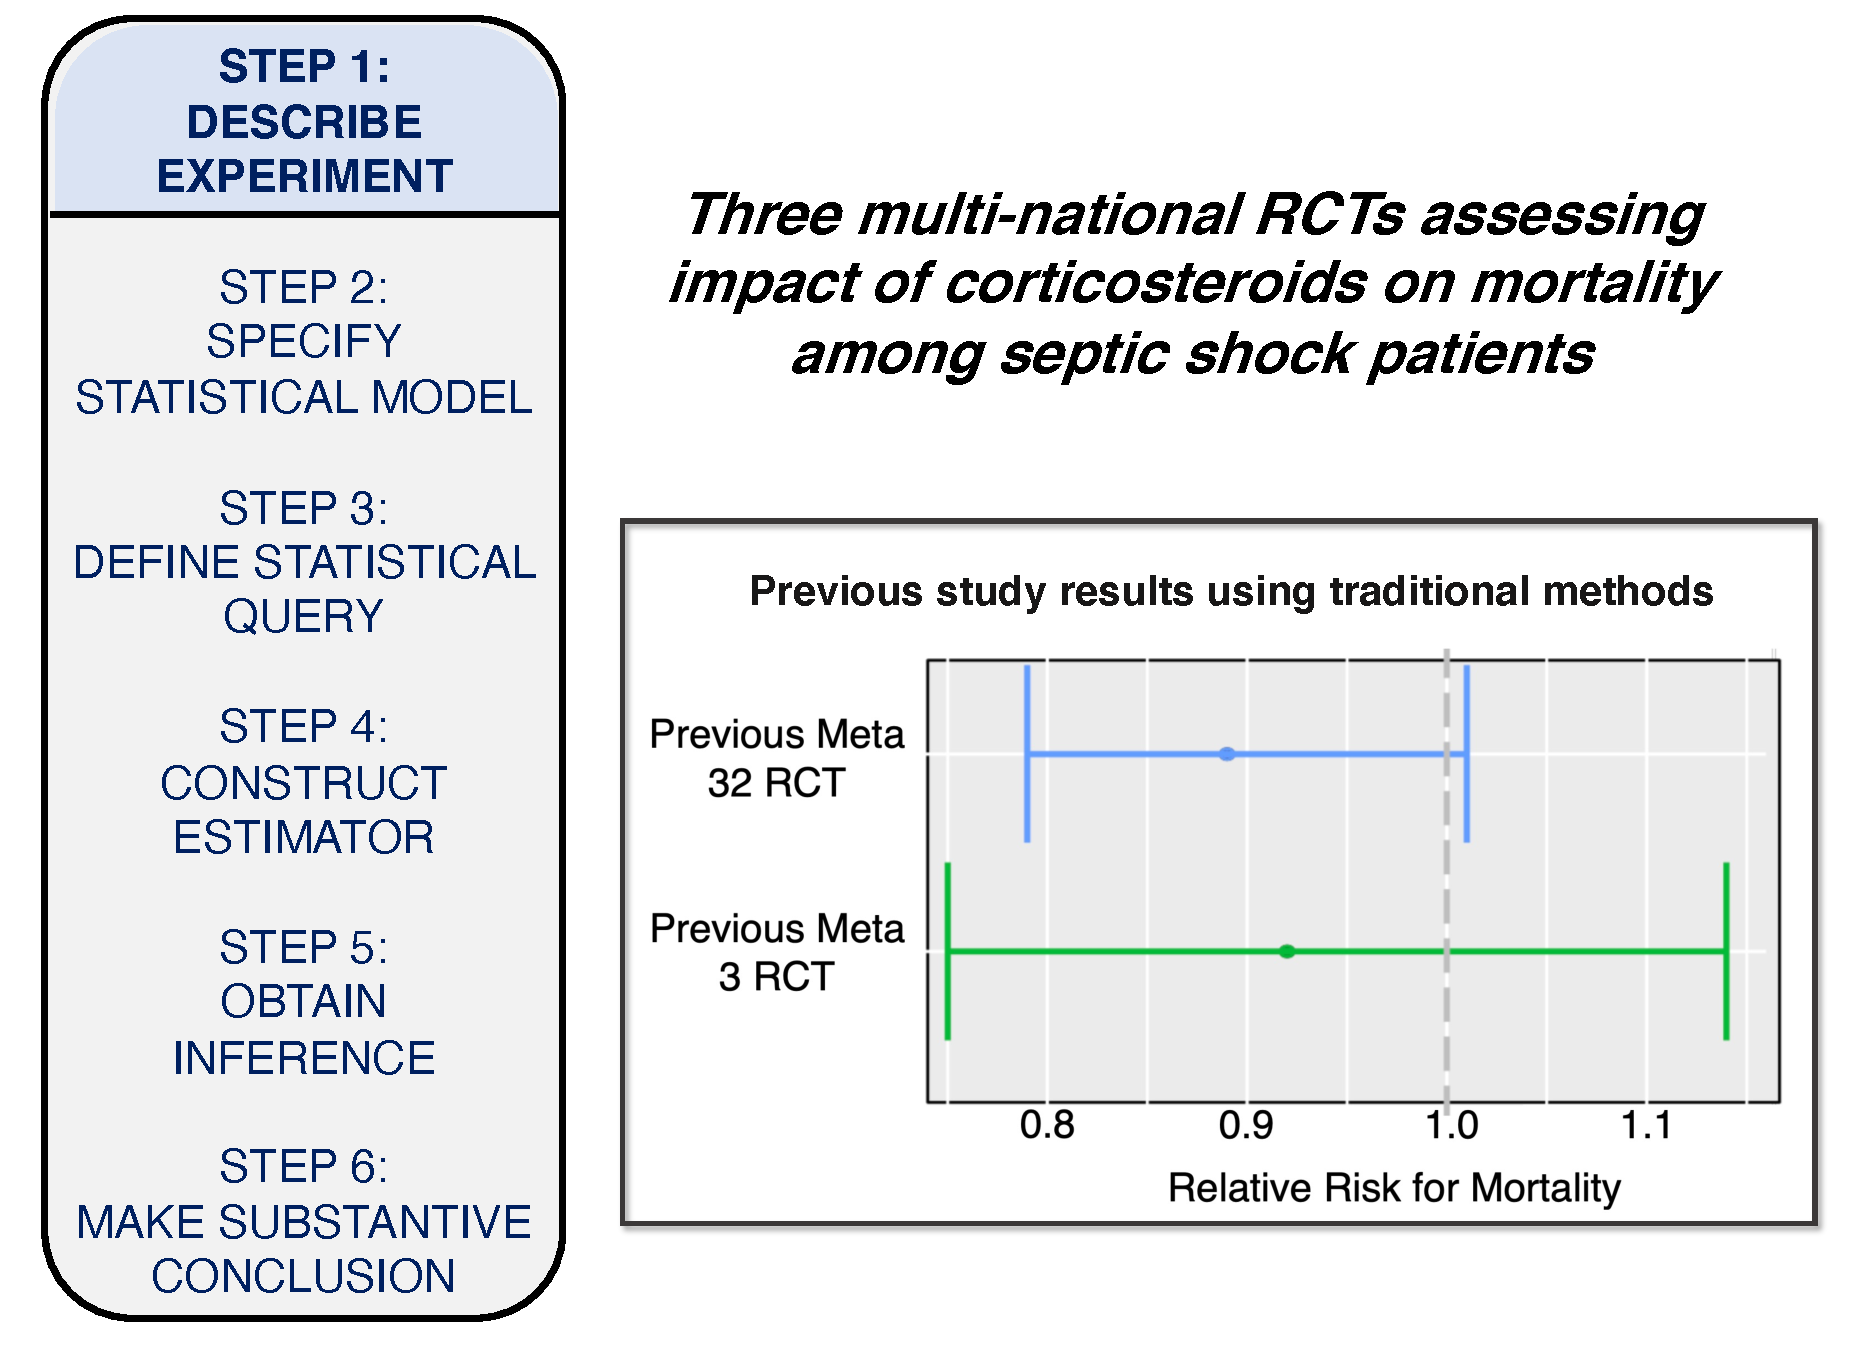
\includegraphics[width = 1.05\textwidth]{figures/roadmap1_1.pdf}
  \end{center}
\end{frame}

\begin{frame}
  \frametitle{Target population of interest}
  \vspace{-20pt}
  \begin{center}
  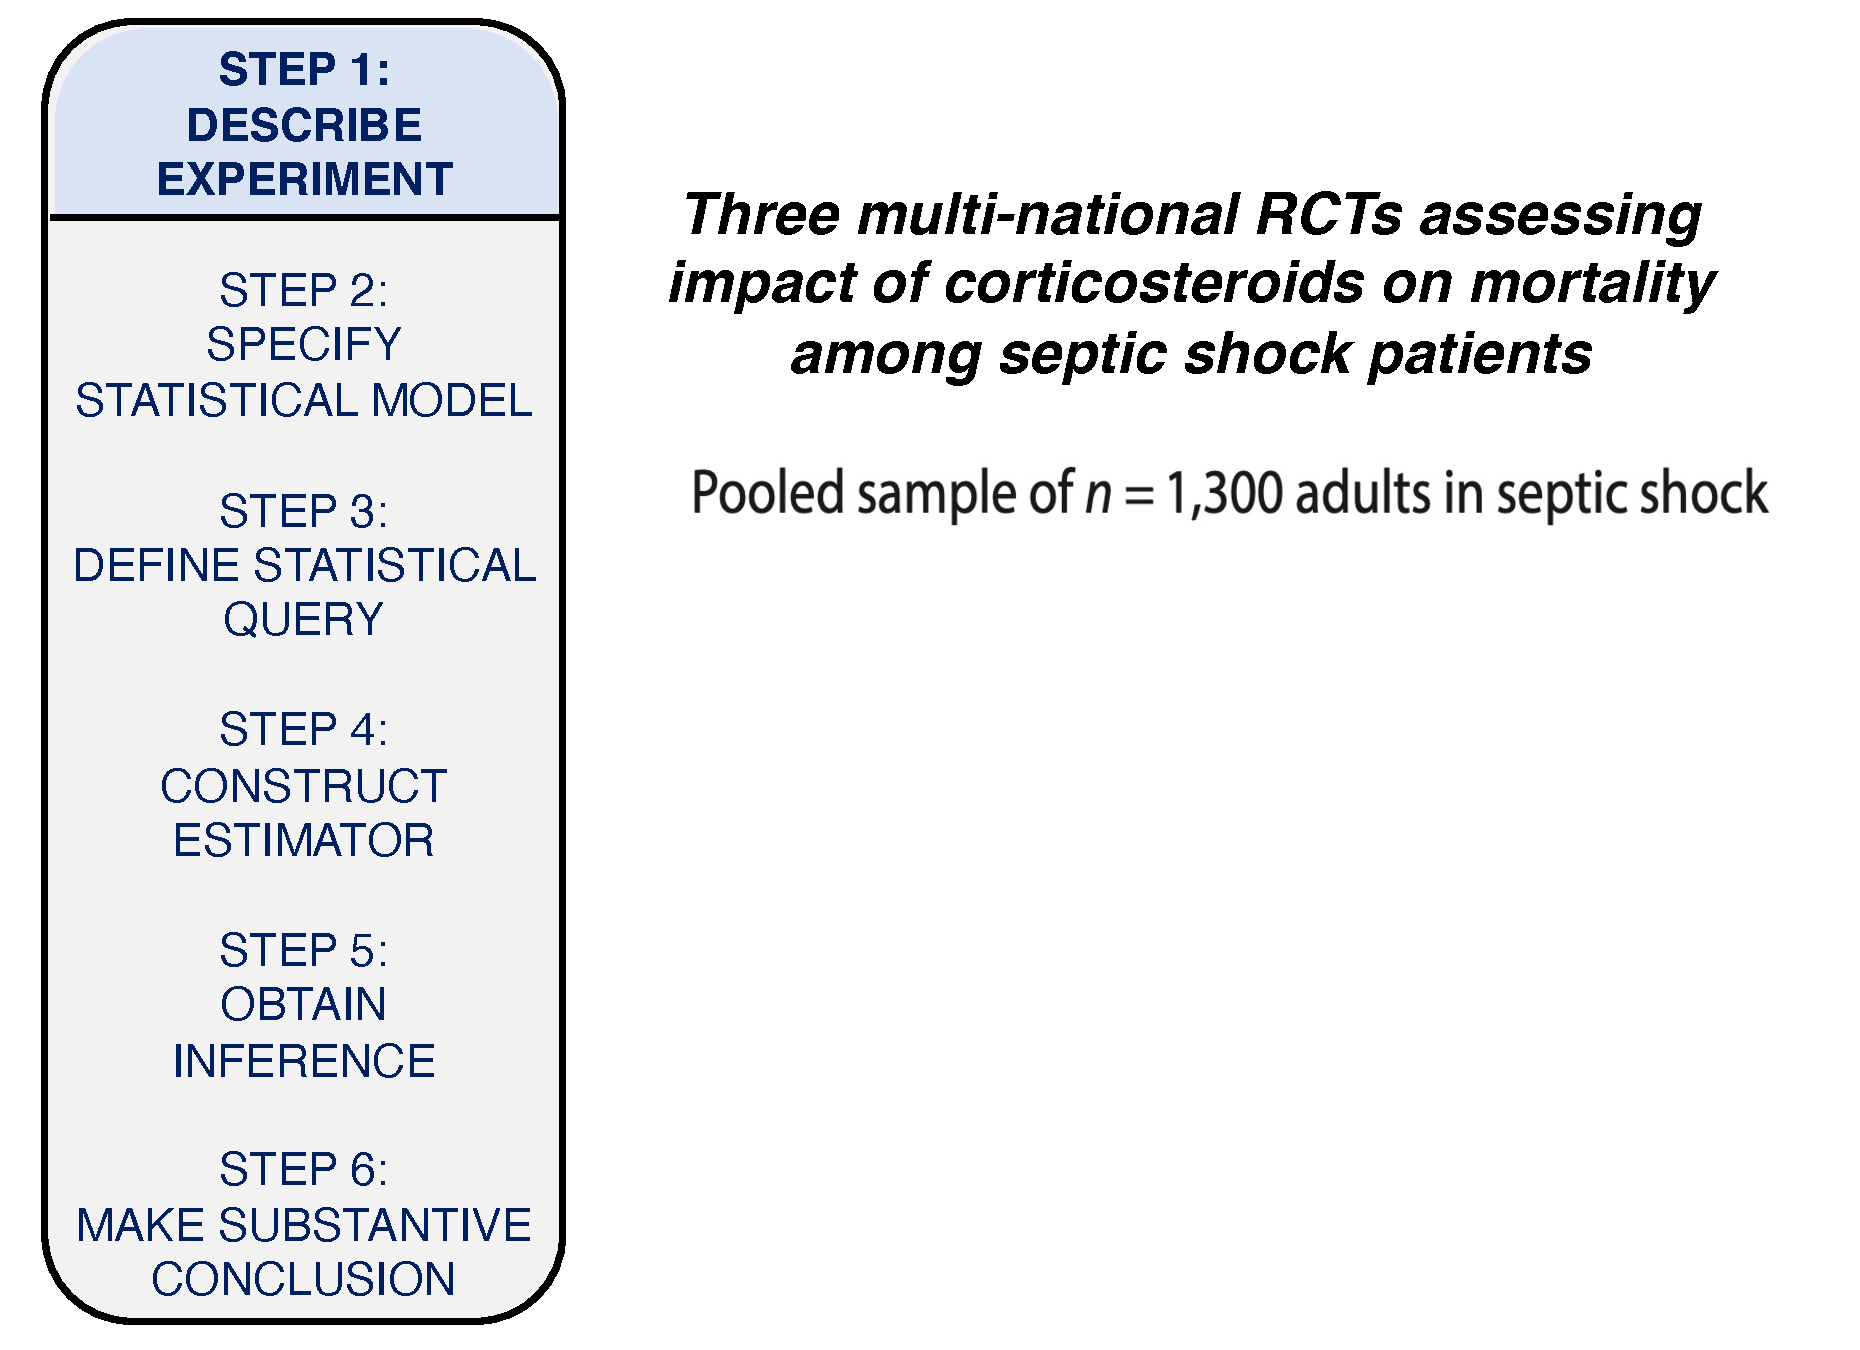
\includegraphics[width = 1.05\textwidth]{figures/data_1.pdf}
  \end{center}
\end{frame}

\begin{frame}
  \frametitle{Observed data structure}
  \vspace{-20pt}
  \begin{center}
  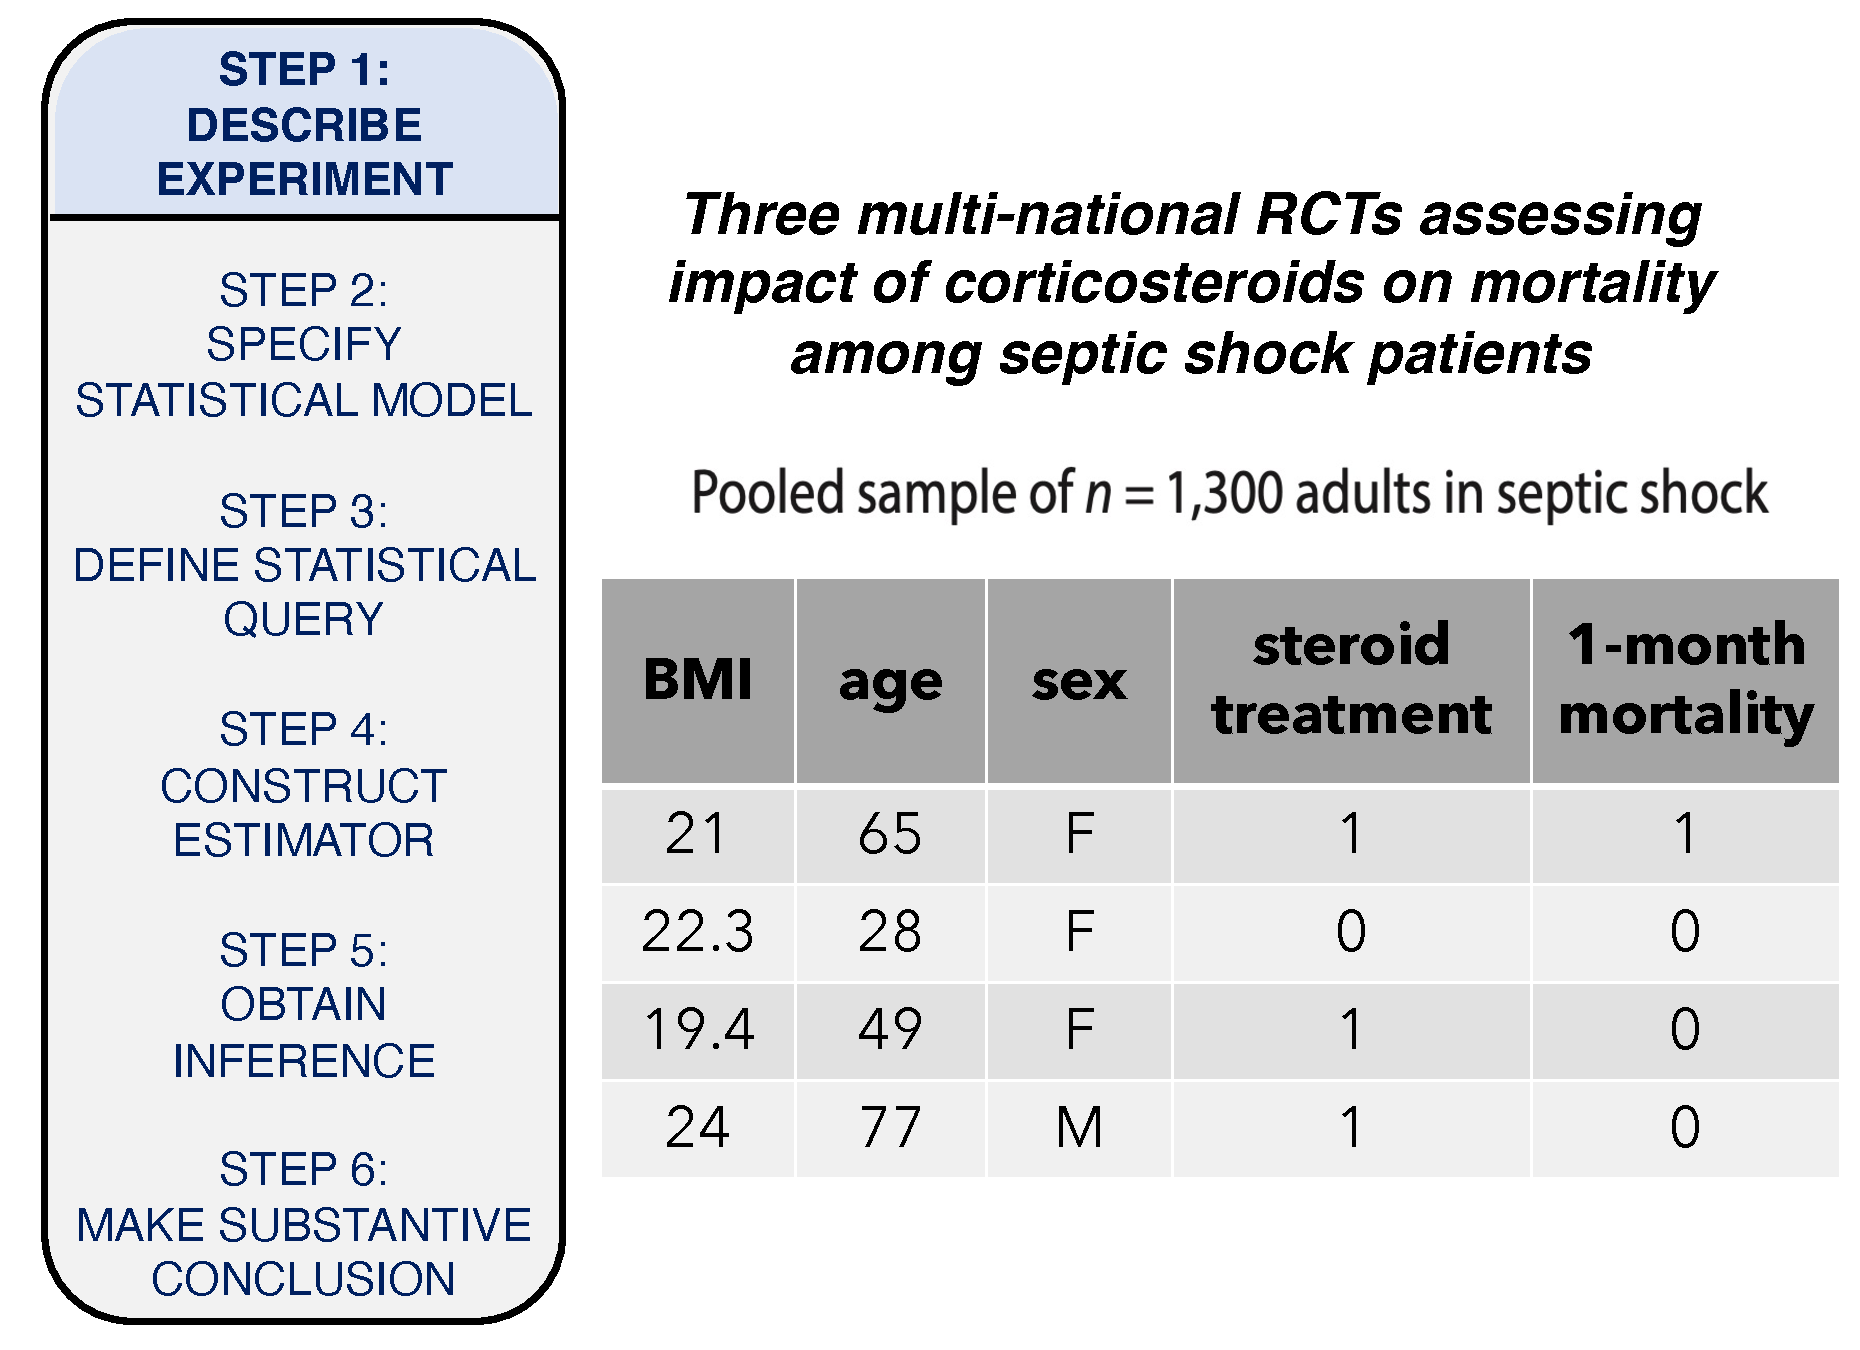
\includegraphics[width = 1.05\textwidth]{figures/data_table.pdf}
  \end{center}
\end{frame}

\begin{frame}
  \frametitle{Directed Acyclic Graph (DAG)}
  \vspace{-20pt}
  \begin{center}
  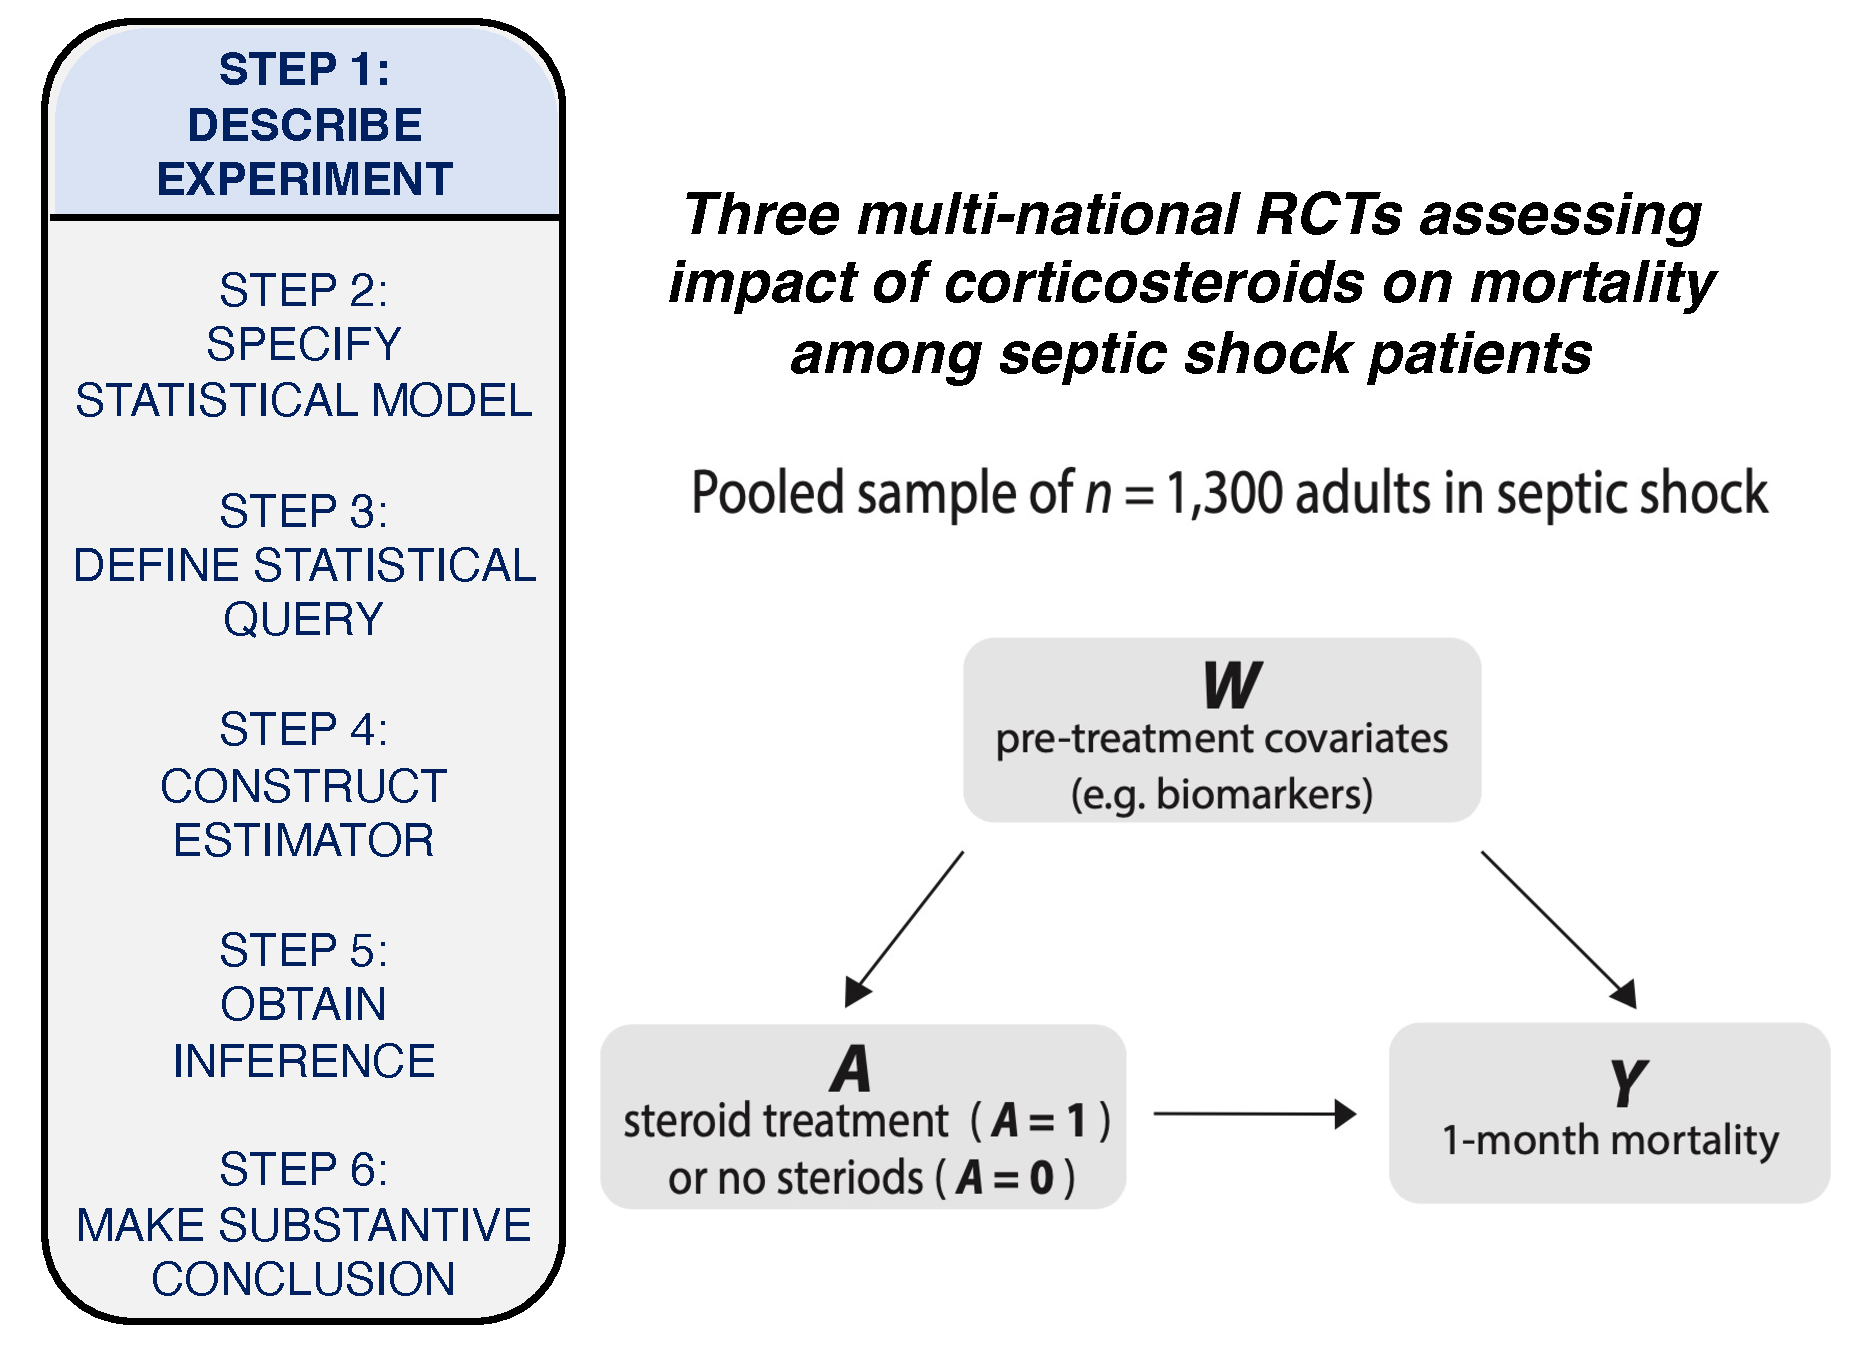
\includegraphics[width = 1.05\textwidth]{figures/DAG.pdf}
  \end{center}
\end{frame}

\subsection{Specify a realistic statistical model}

\begin{frame}
  \frametitle{Step 2: What is known about stochastic relations of the observed variables?}
  \vspace{-20pt}
  \begin{center}
  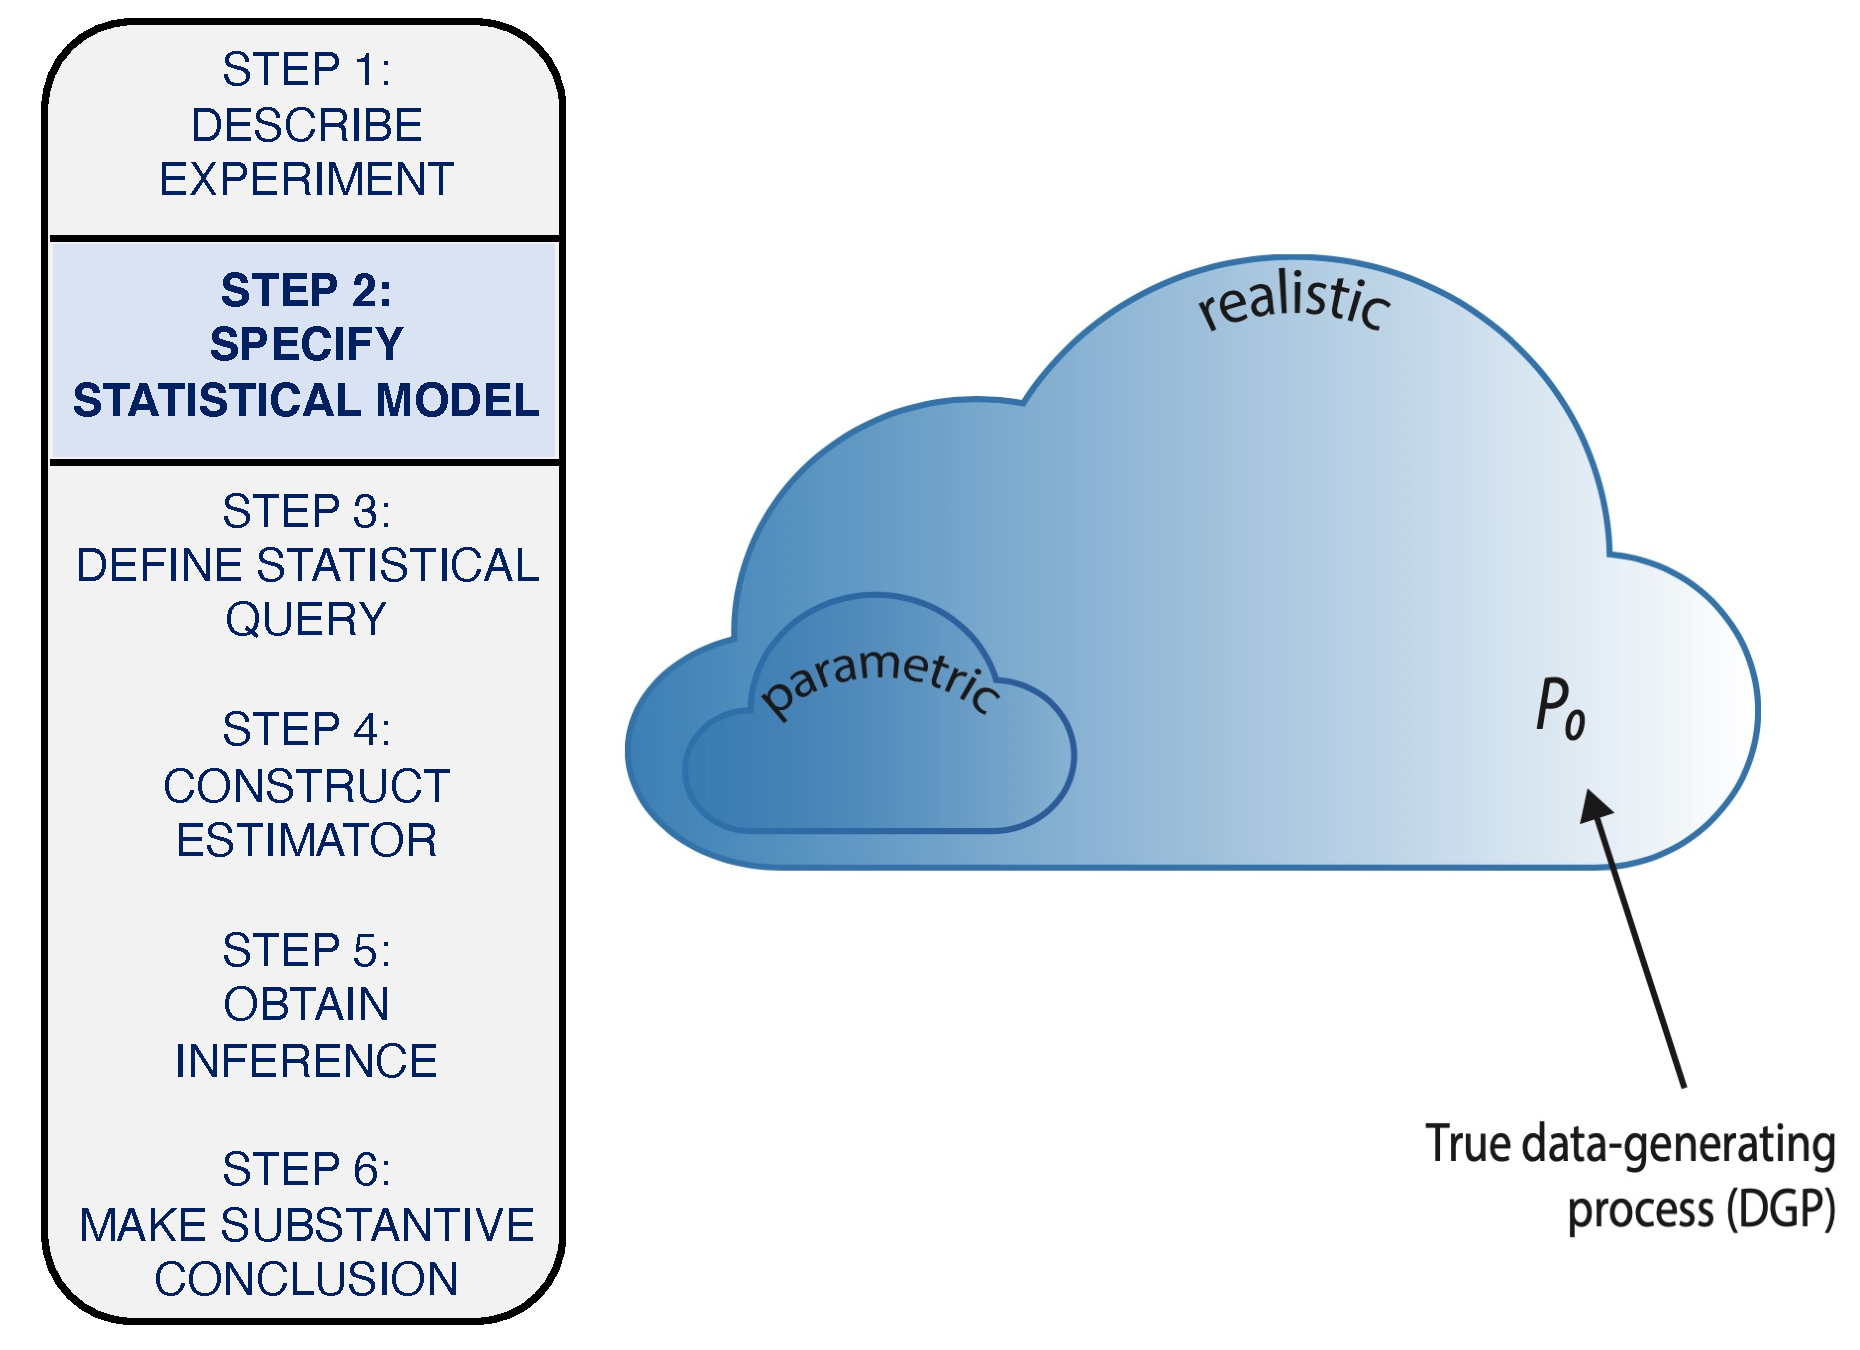
\includegraphics[width = 1.05\textwidth]{figures/roadmap2.pdf}
  \end{center}
\end{frame}

\begin{frame}
\frametitle{What happens when the statistical model is misspecified (i.e. does not contain $P_0$, the DGP)?}
\vspace{15pt}
\centering
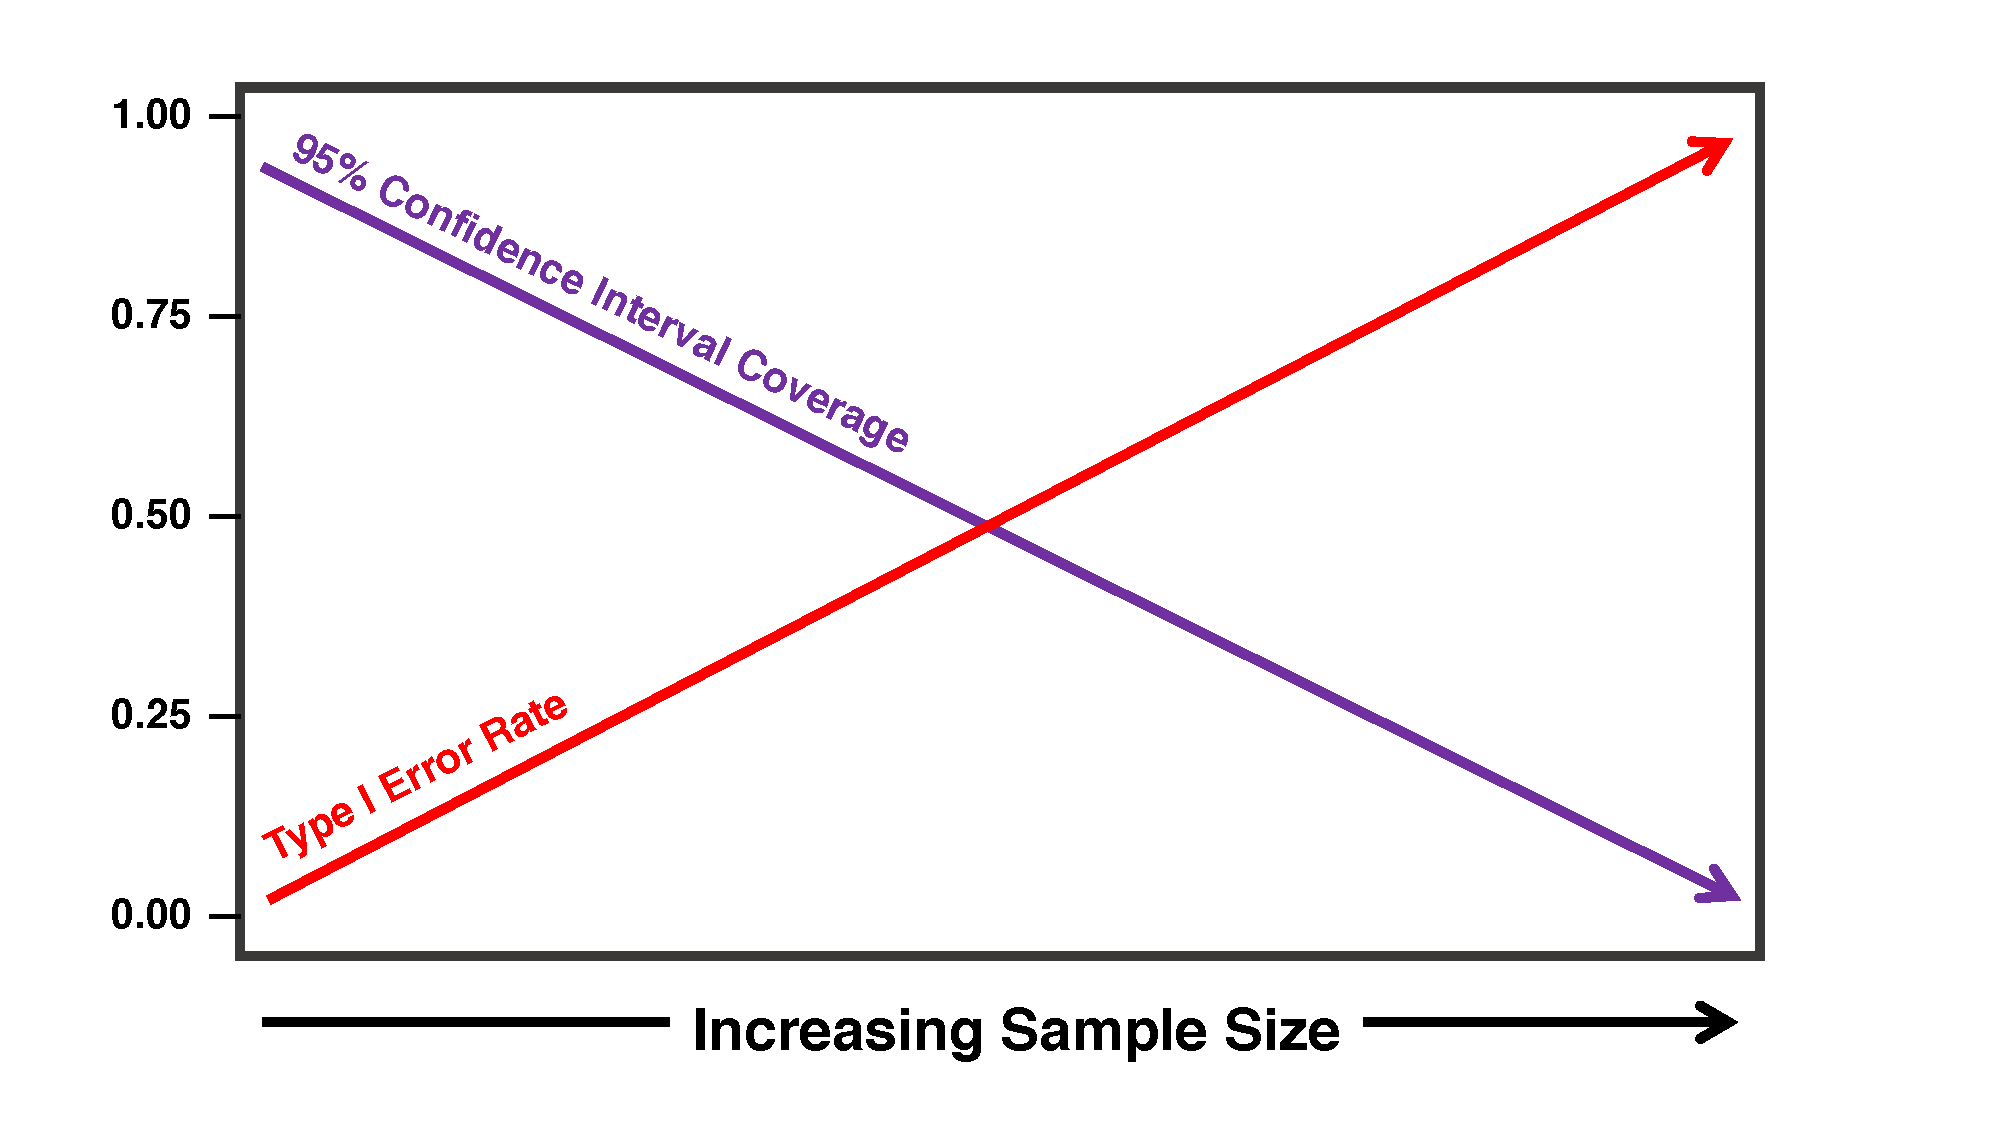
\includegraphics[width=1.05\textwidth]{figures/misspecified.pdf}
\end{frame}

\subsection{Define estimand}

\subsubsection{Causal estimand}
\begin{frame}
  \frametitle{Step 3a: What is the target causal estimand that we aim to identify from the data?}
  % defining full-data
  \vspace{-20pt}
  \begin{center}
  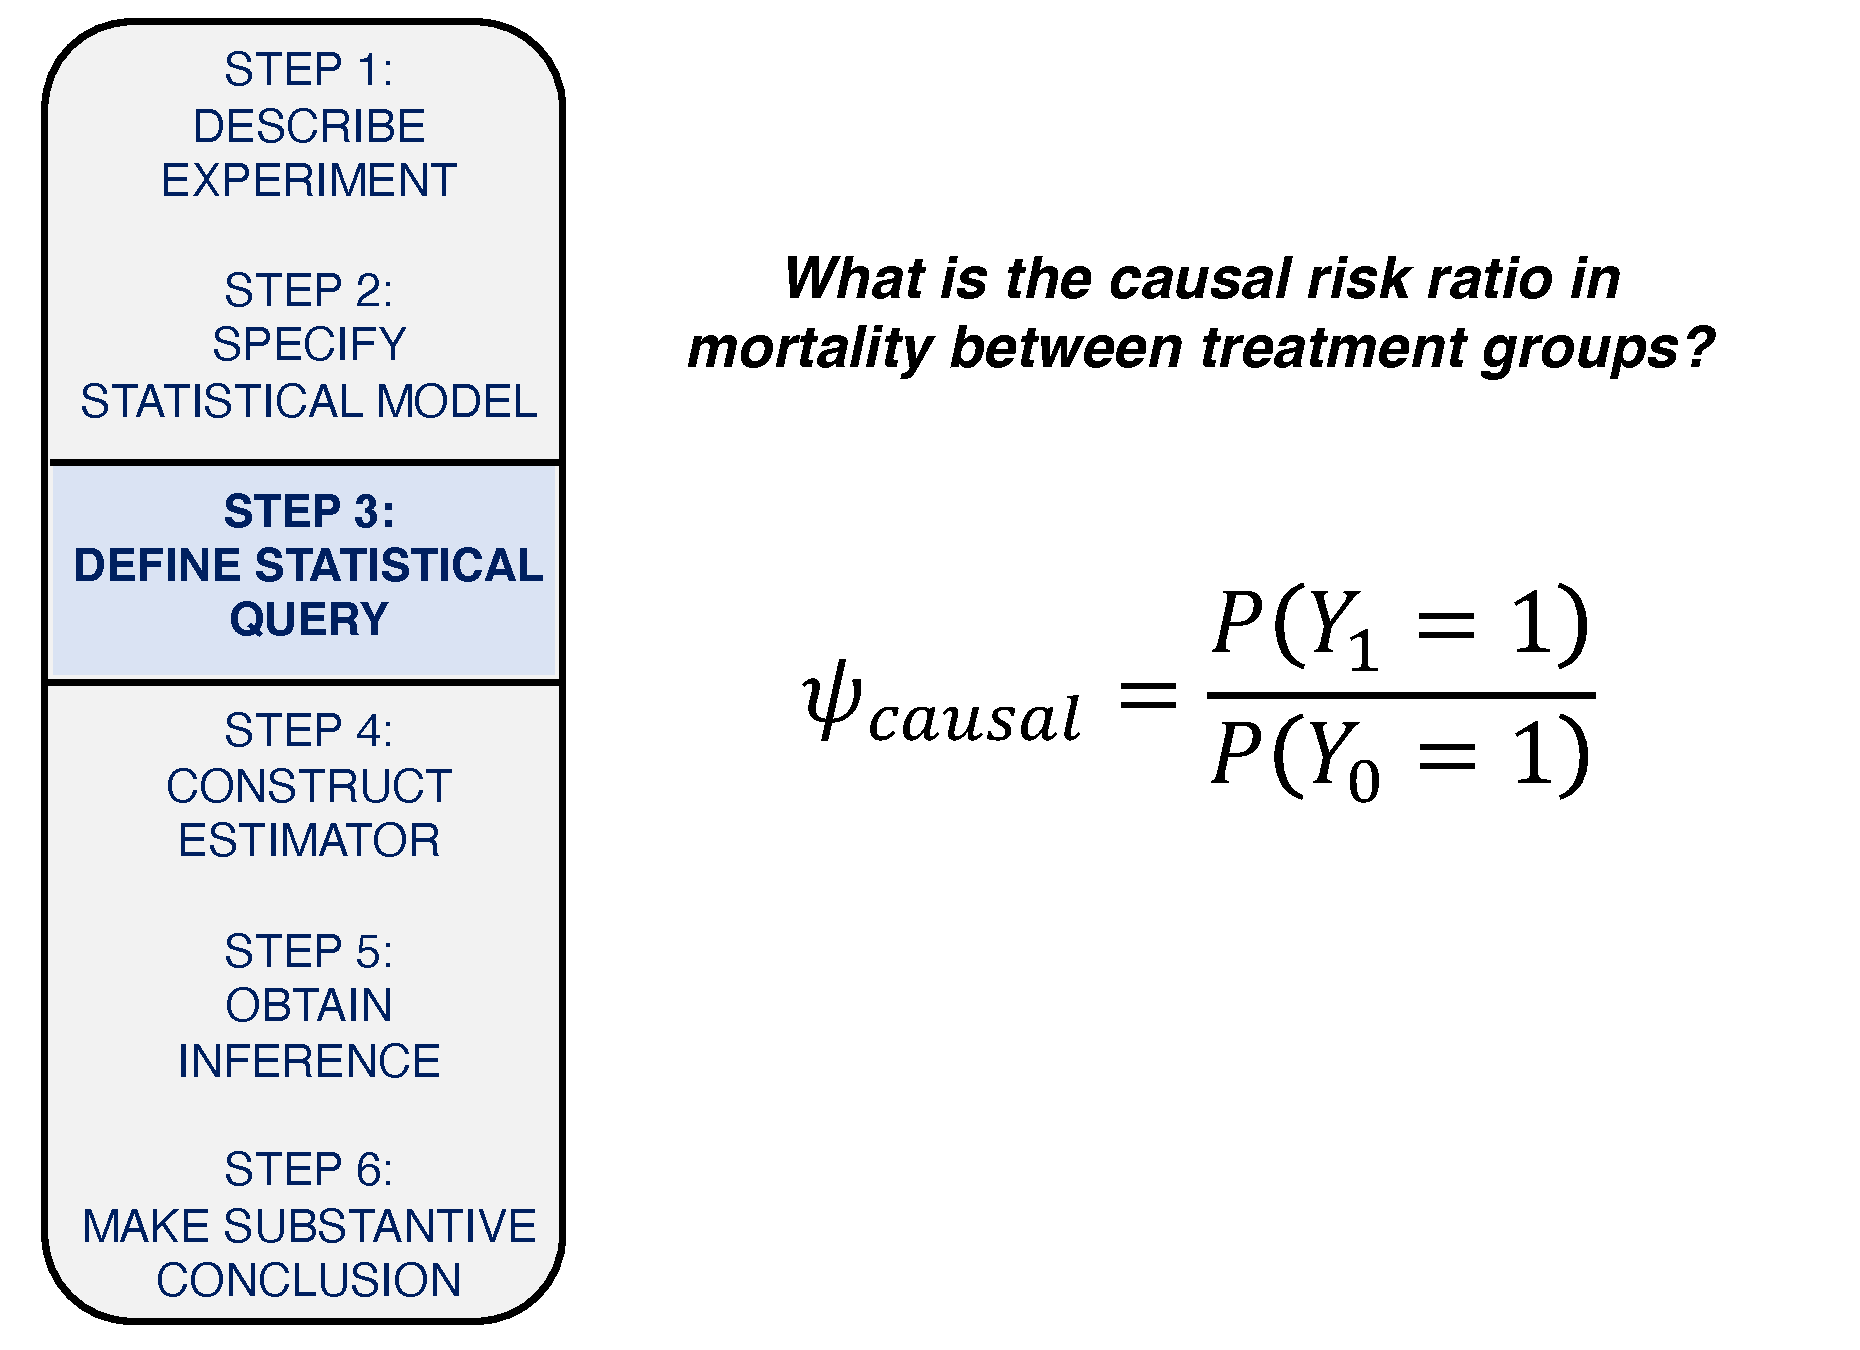
\includegraphics[width = 1.05\textwidth]{figures/causalRR.pdf}
  \end{center}
\end{frame}

\begin{frame}
  \frametitle{Proportion of subjects in the population of interest that would have died had they all received steroids}
  % defining full-data
  \vspace{-20pt}
  \begin{center}
  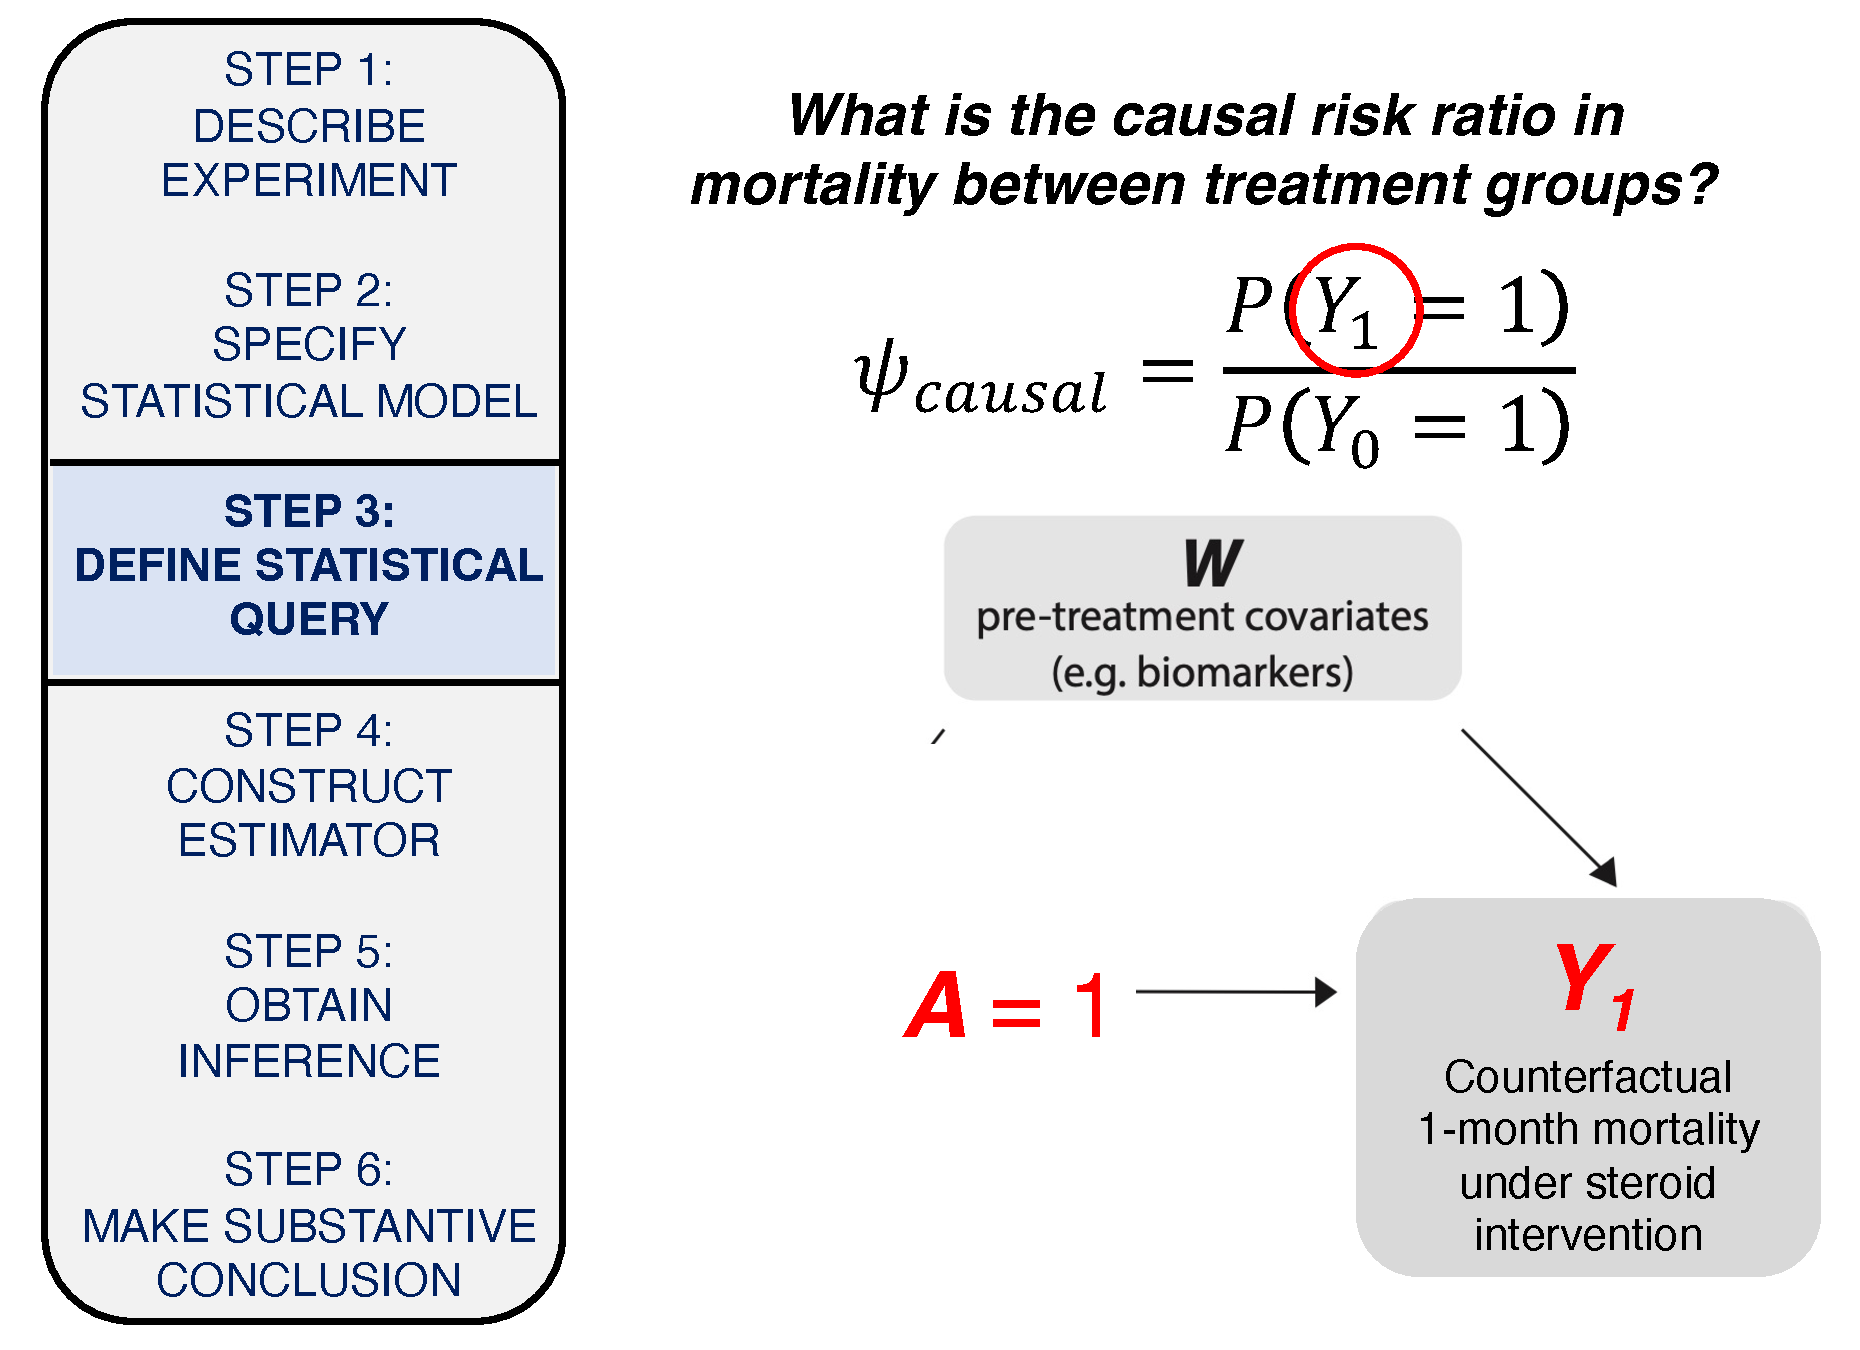
\includegraphics[width = 1.05\textwidth]{figures/counterfactual_Y1.pdf}
  \end{center}
\end{frame}

\begin{frame}
  \frametitle{Proportion of subjects in the target population that would have died had they all not received steroids}
  % defining full-data
  \vspace{-20pt}
  \begin{center}
  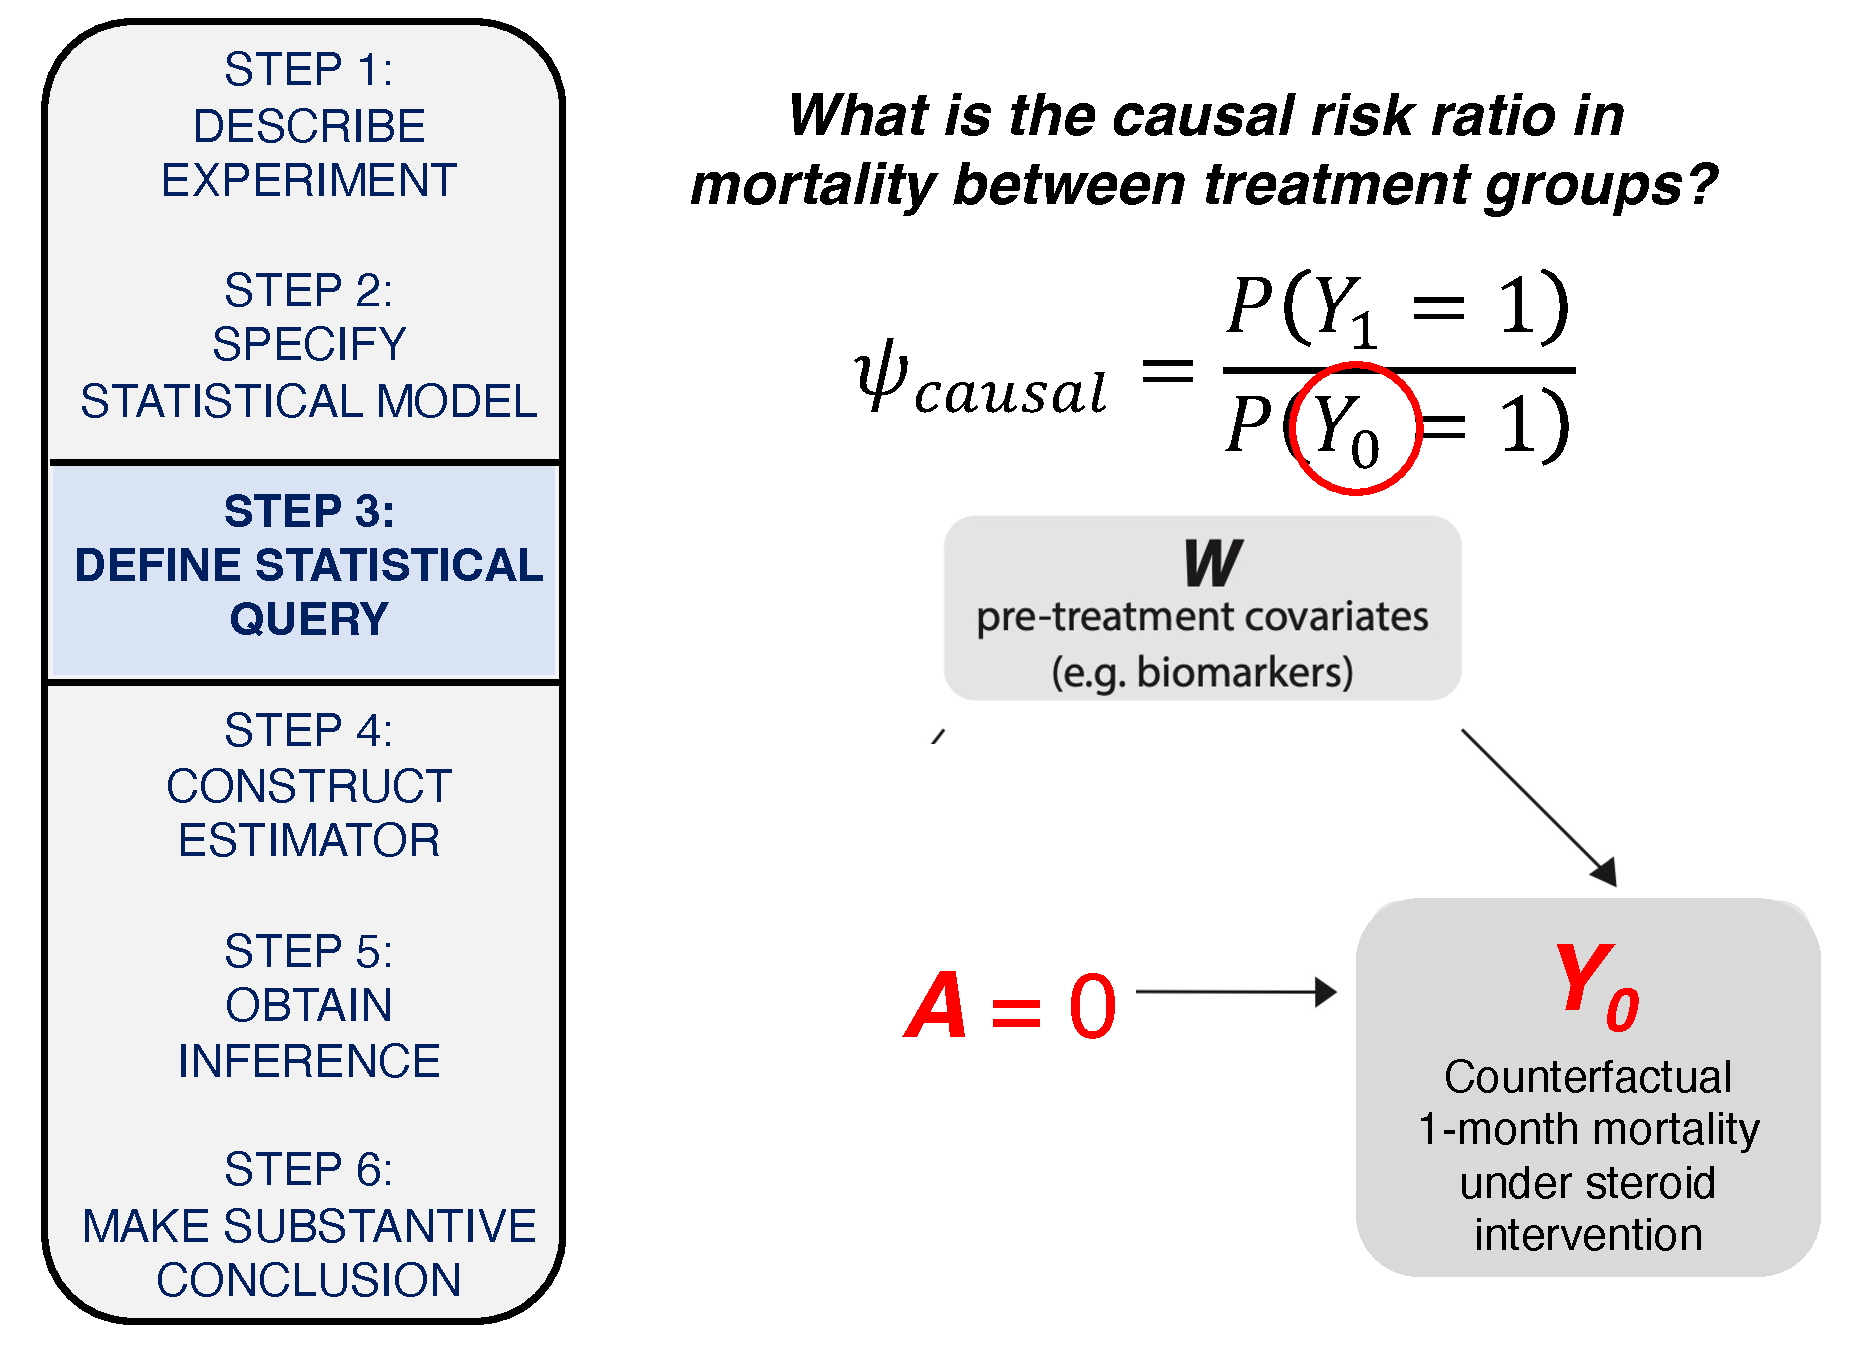
\includegraphics[width = 1.05\textwidth]{figures/counterfactual_Y0.pdf}
  \end{center}
\end{frame}

\begin{frame}
  \frametitle{Causal target parameters are functions of the full data under the intervention(s) of interest}
  % defining full-data
  \vspace{-20pt}
  \begin{center}
  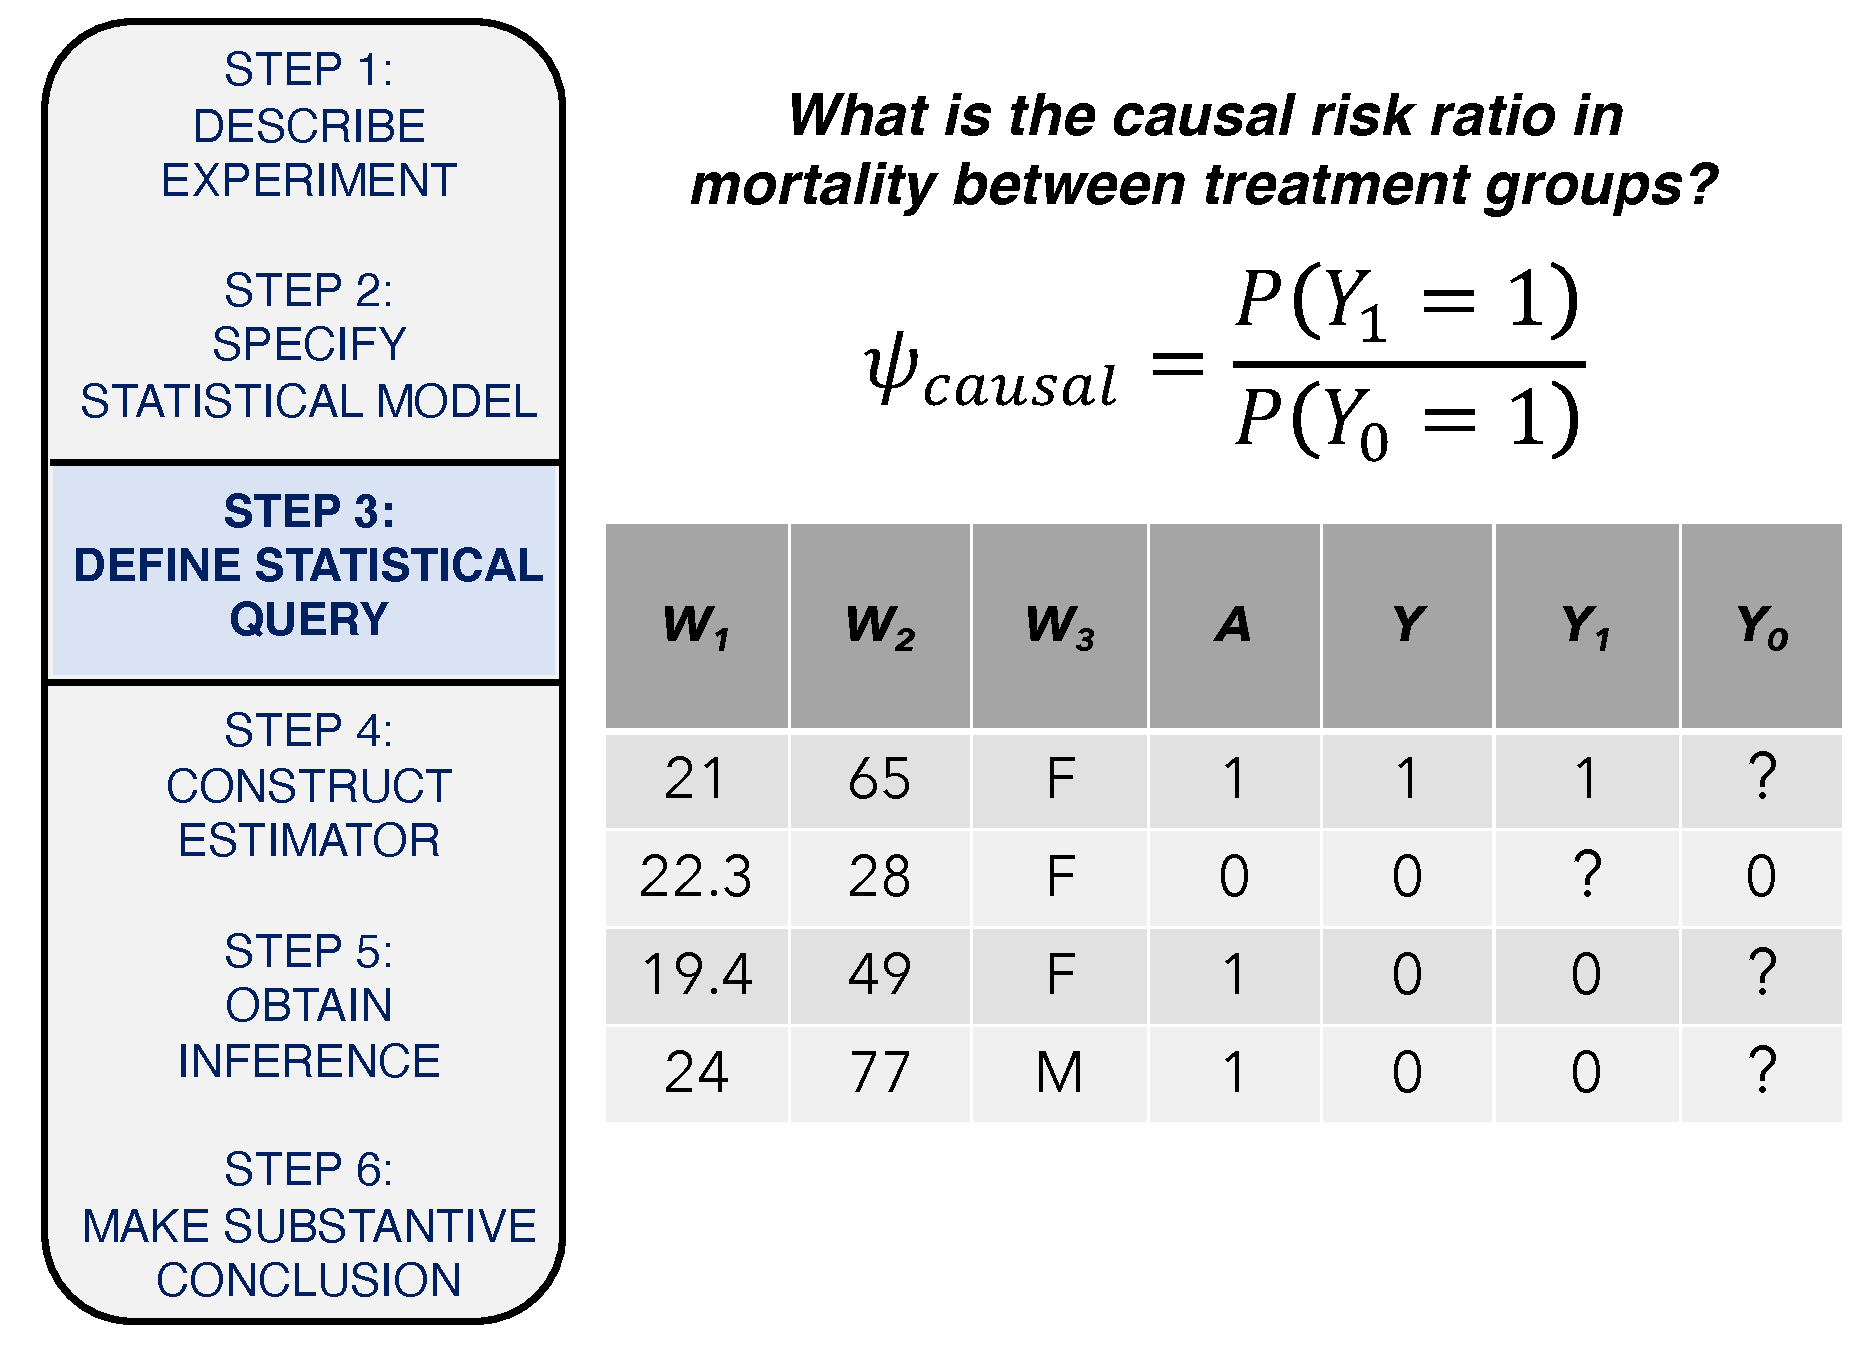
\includegraphics[width = 1.05\textwidth]{figures/causalRR_fulldata1.pdf}
  \end{center}
\end{frame}

%\begin{frame}
 % \frametitle{Step 3a: What is the target causal estimand that we aim to identify from the data?}
  % defining full-data
 % \vspace{-20pt}
  %\begin{center}
 % 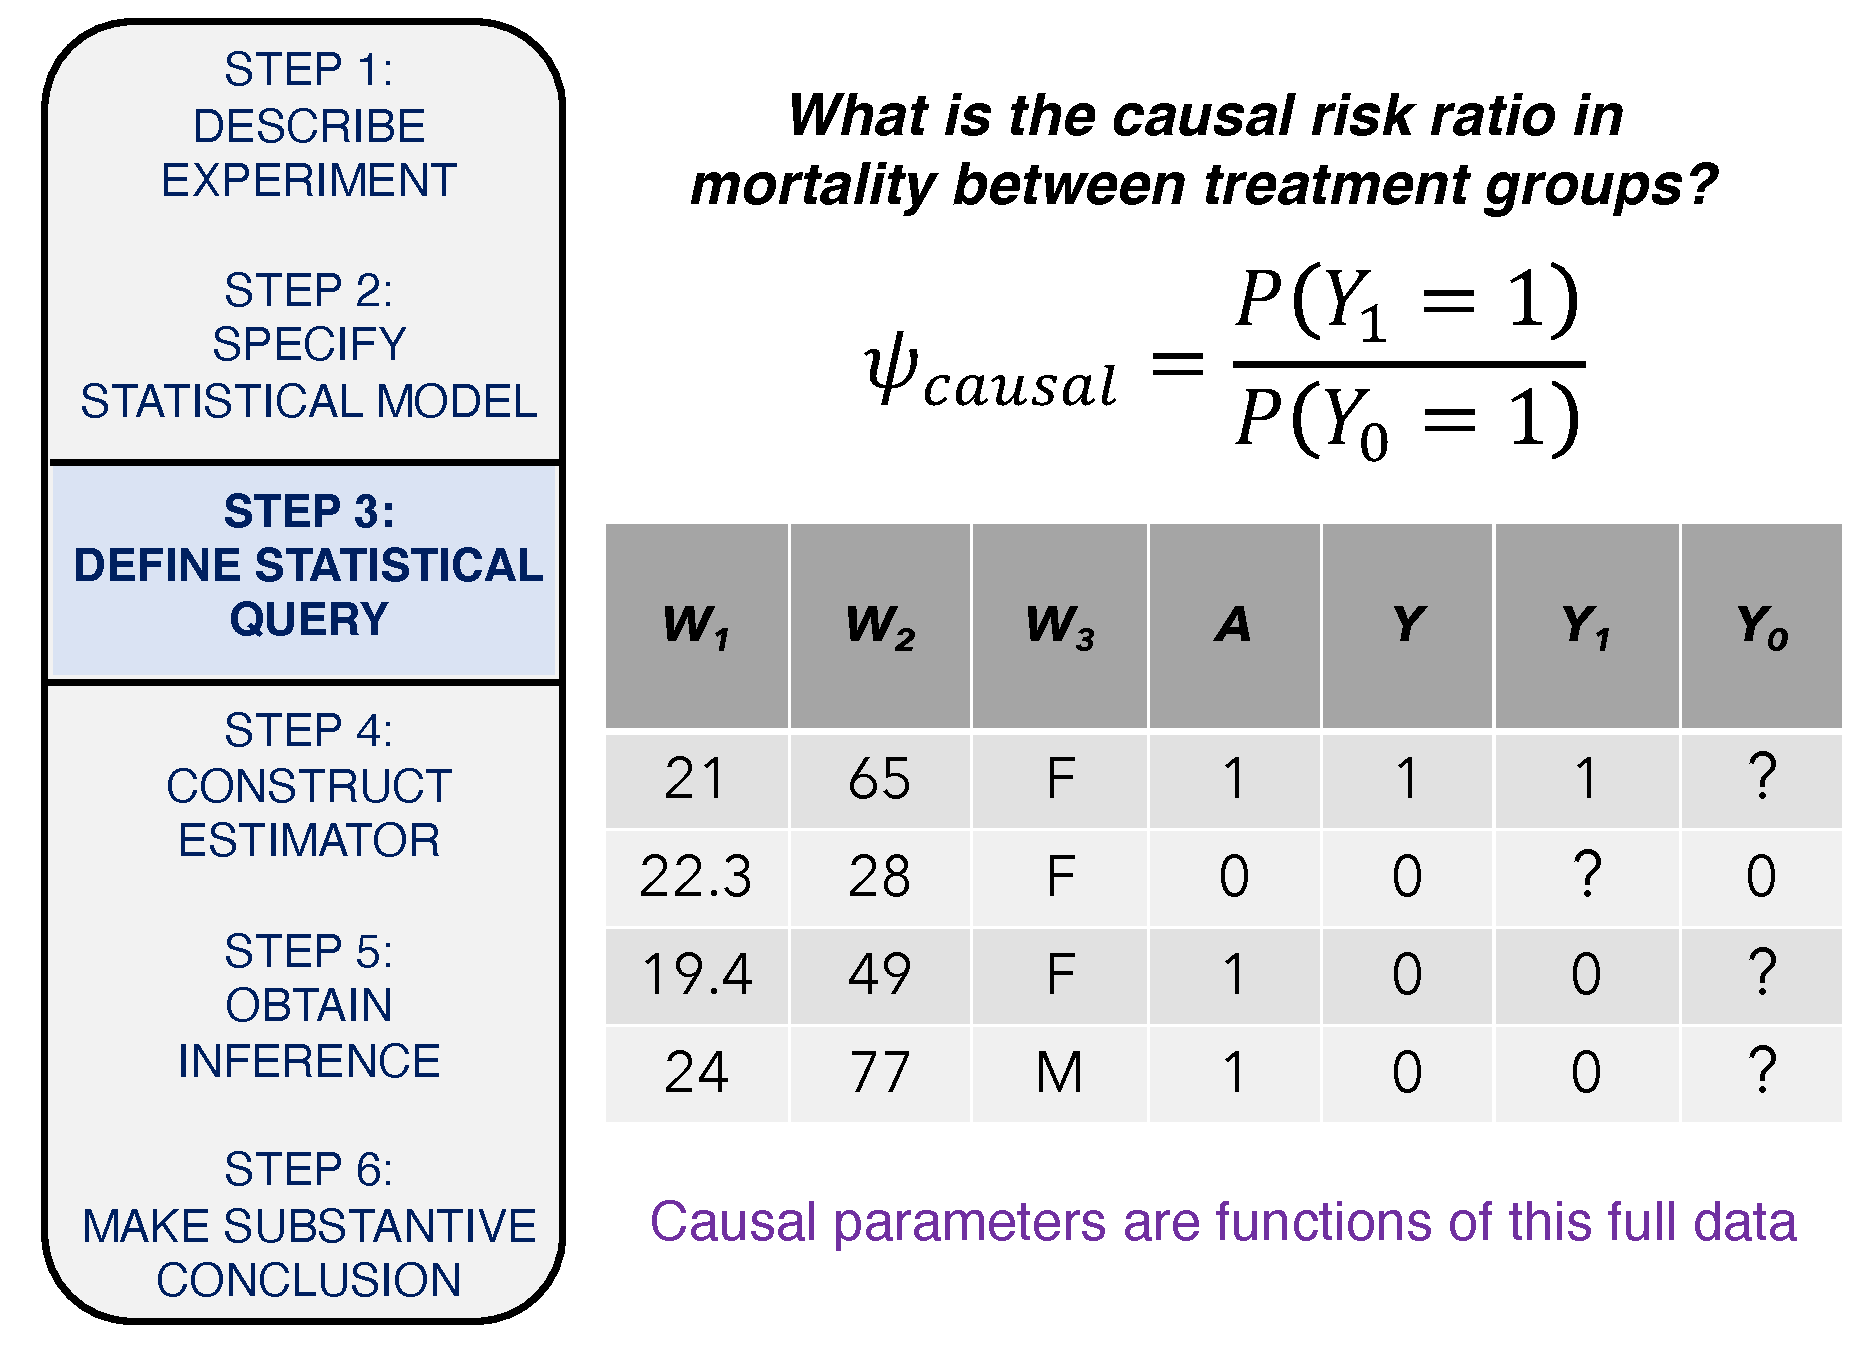
\includegraphics[width = 1.05\textwidth]{figures/causalRR_fulldata2.pdf}
 % \end{center}
% \end{frame}

\begin{frame}
  \frametitle{Causal identifiability assumptions must hold in order to interpret the estimate causally}
  % defining full-data
  \vspace{-20pt}
  \begin{center}
  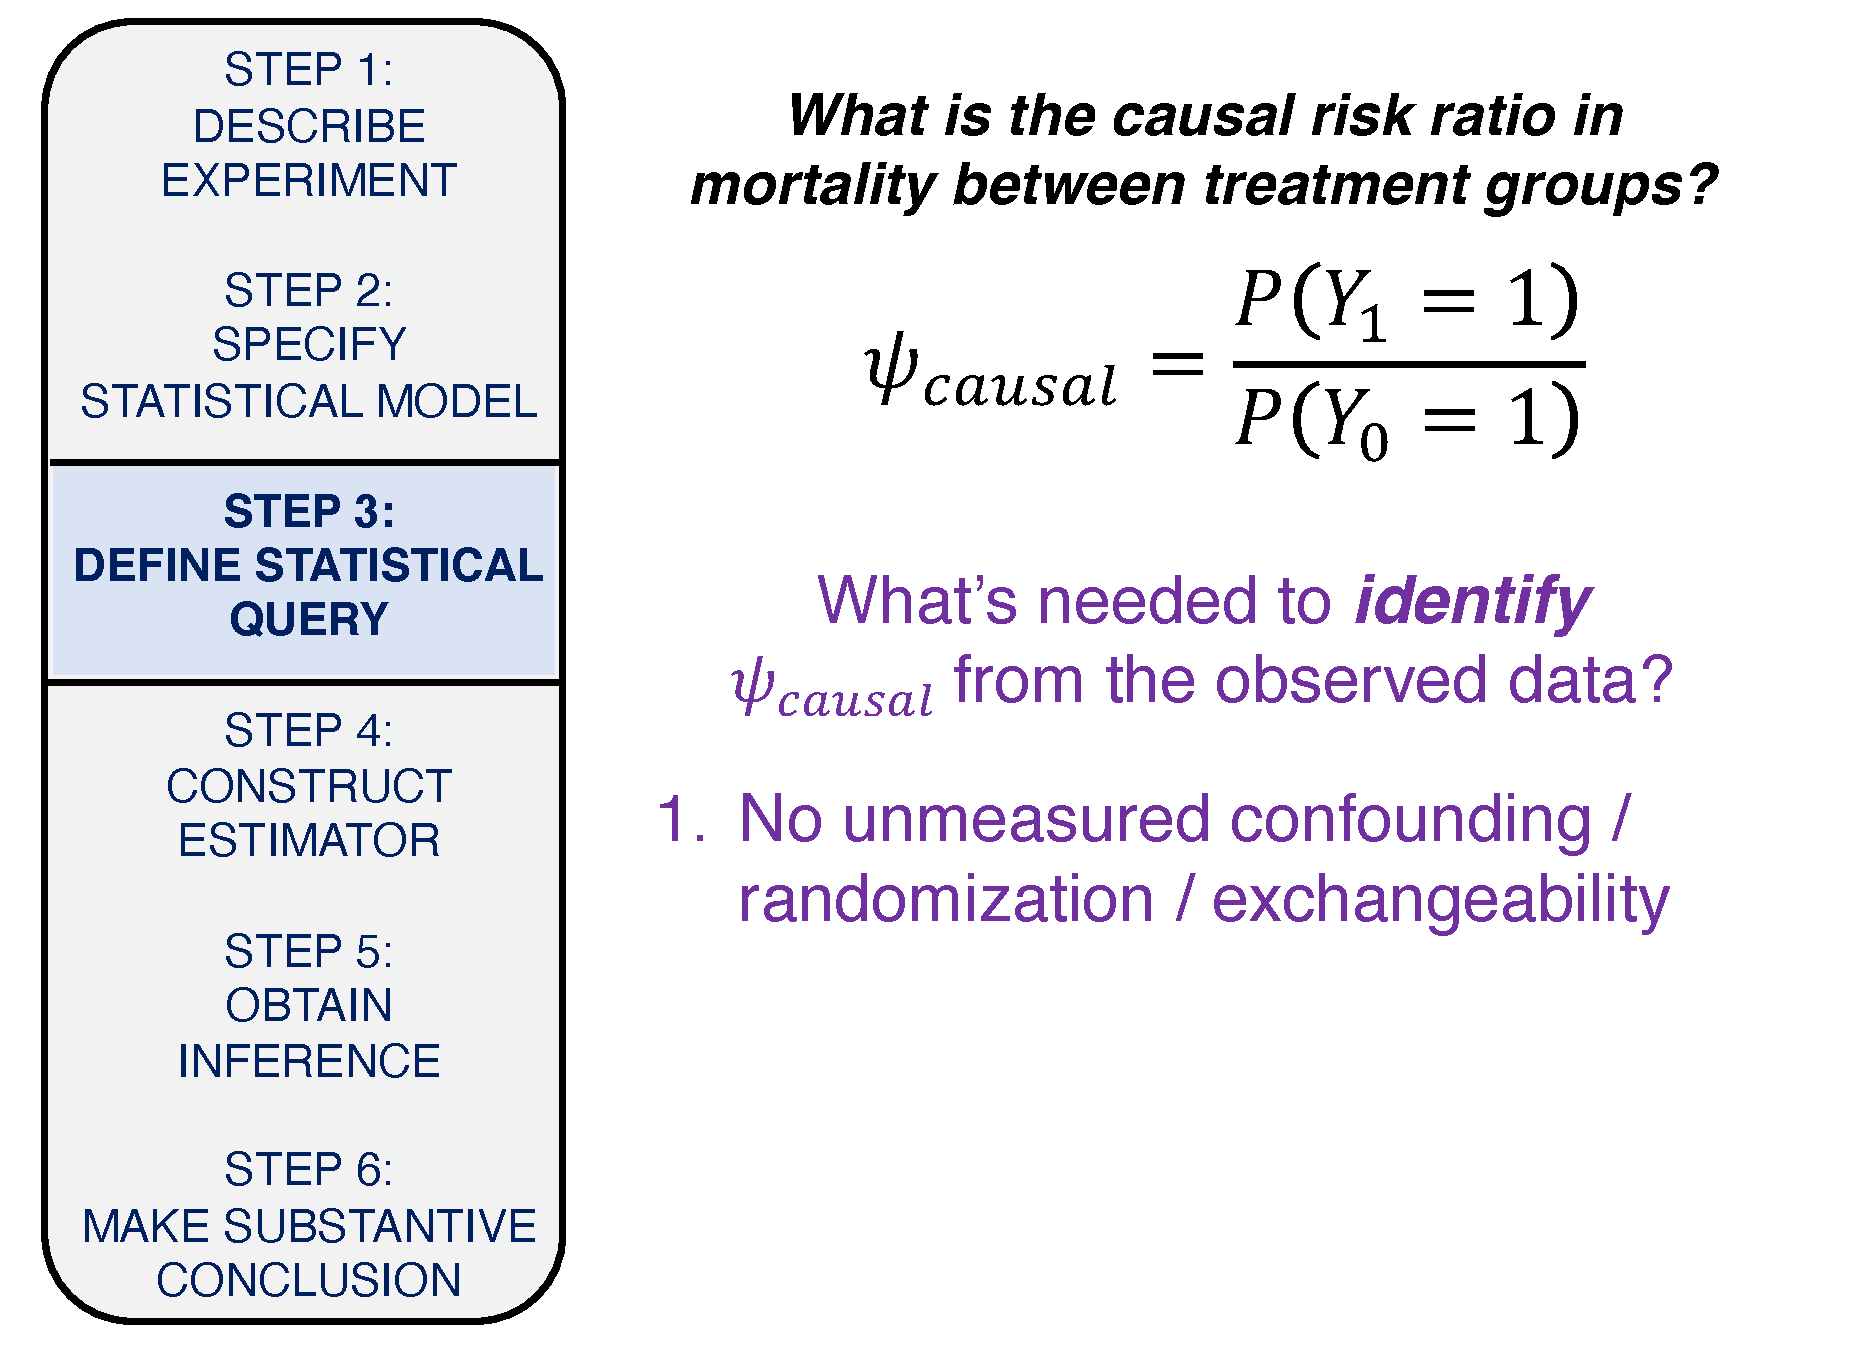
\includegraphics[width = 1.05\textwidth]{figures/causalRR_identify1.pdf}
  \end{center}
\end{frame}

\begin{frame}
  \frametitle{Some causal identifiability assumptions are also necessary for well-defined statistical esitmation}
  % defining full-data
  \vspace{-20pt}
  \begin{center}
  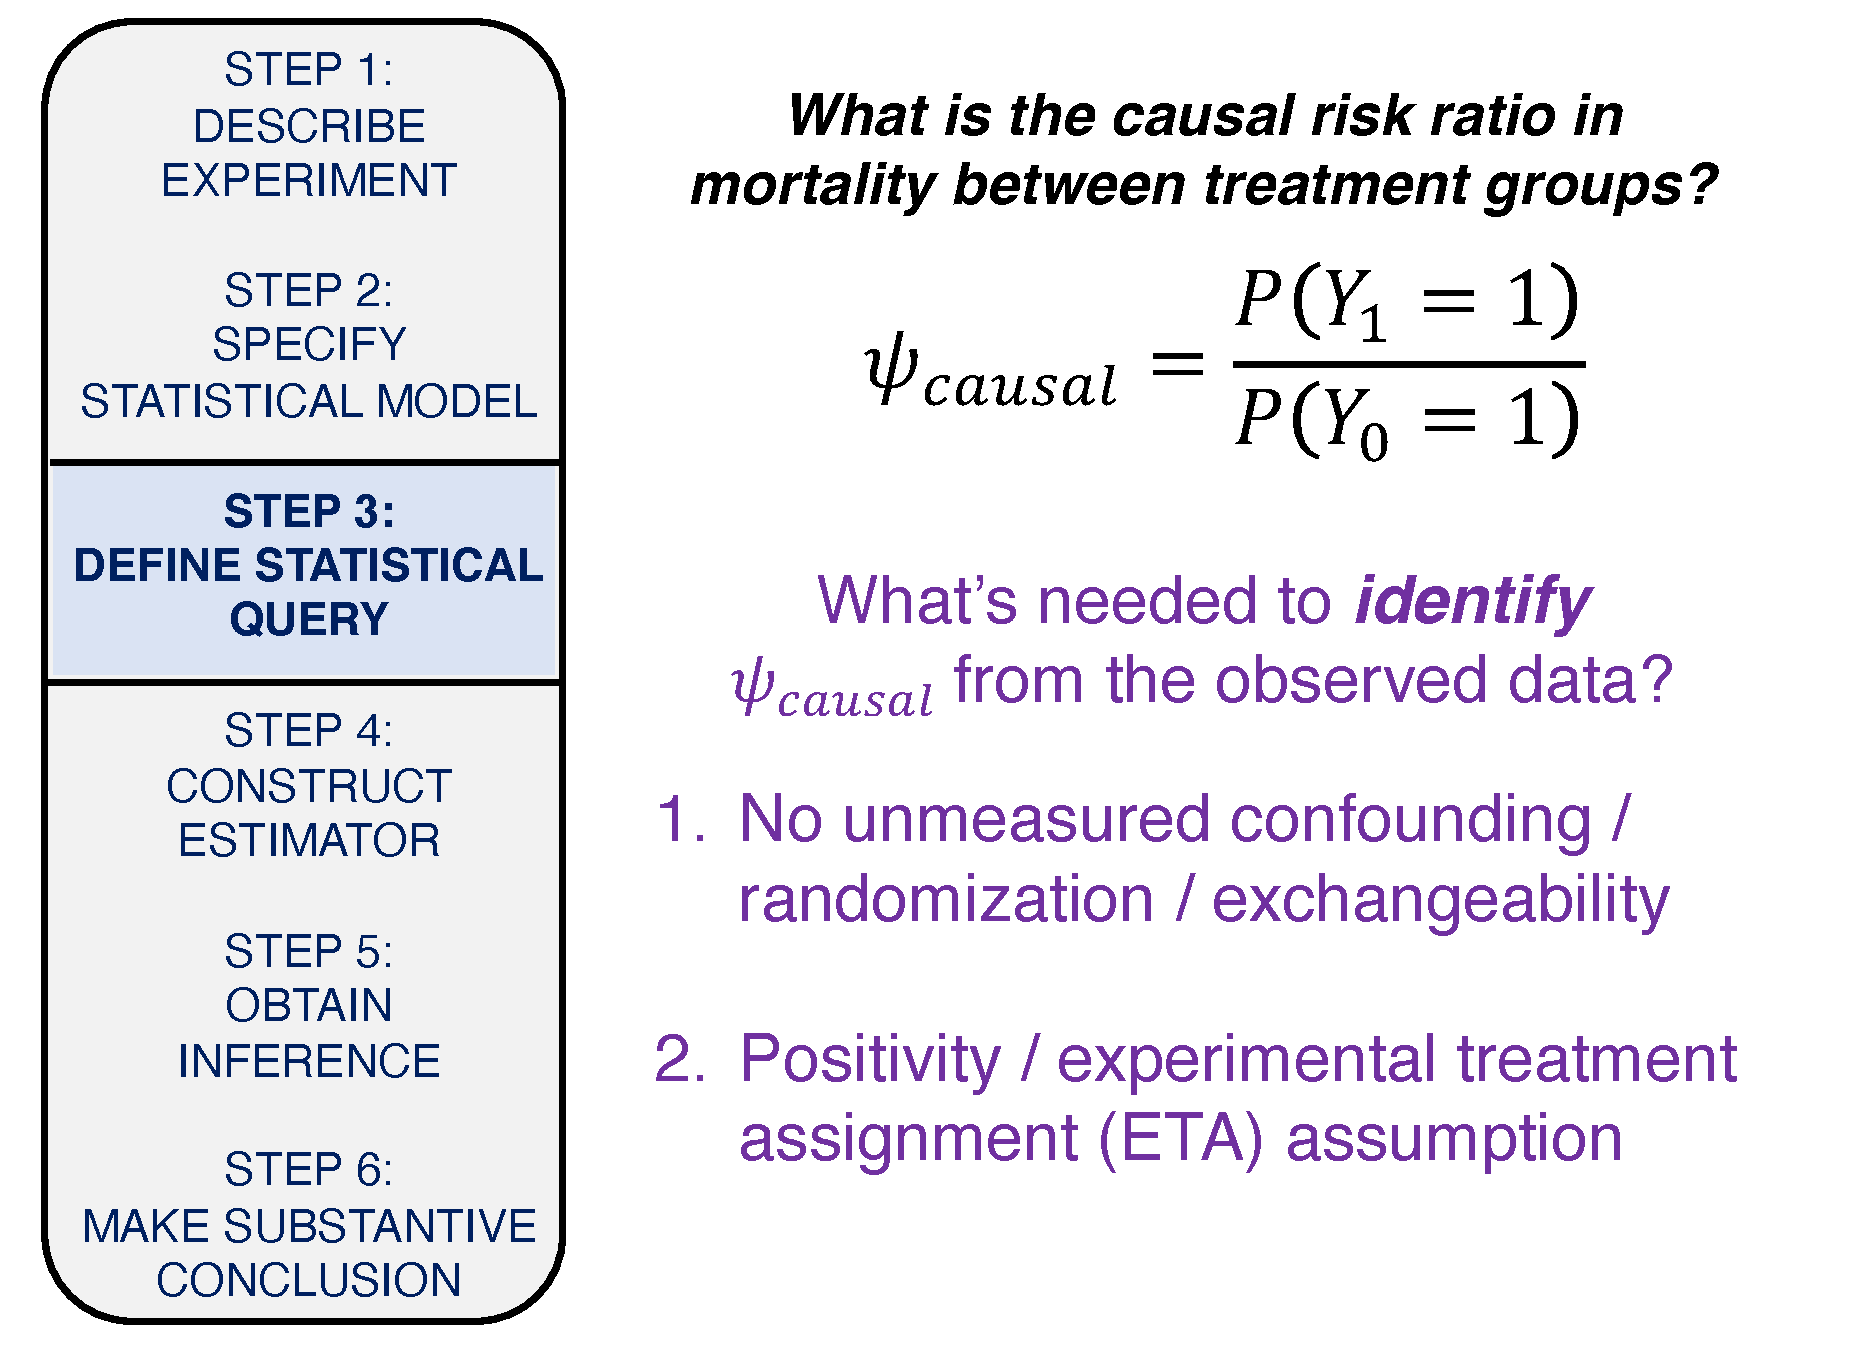
\includegraphics[width = 1.05\textwidth]{figures/causalRR_identify2.pdf}
  \end{center}
\end{frame}

\begin{frame}
  \frametitle{Identification formula from g-computation}
  % defining full-data
  \vspace{-20pt}
  \begin{center}
  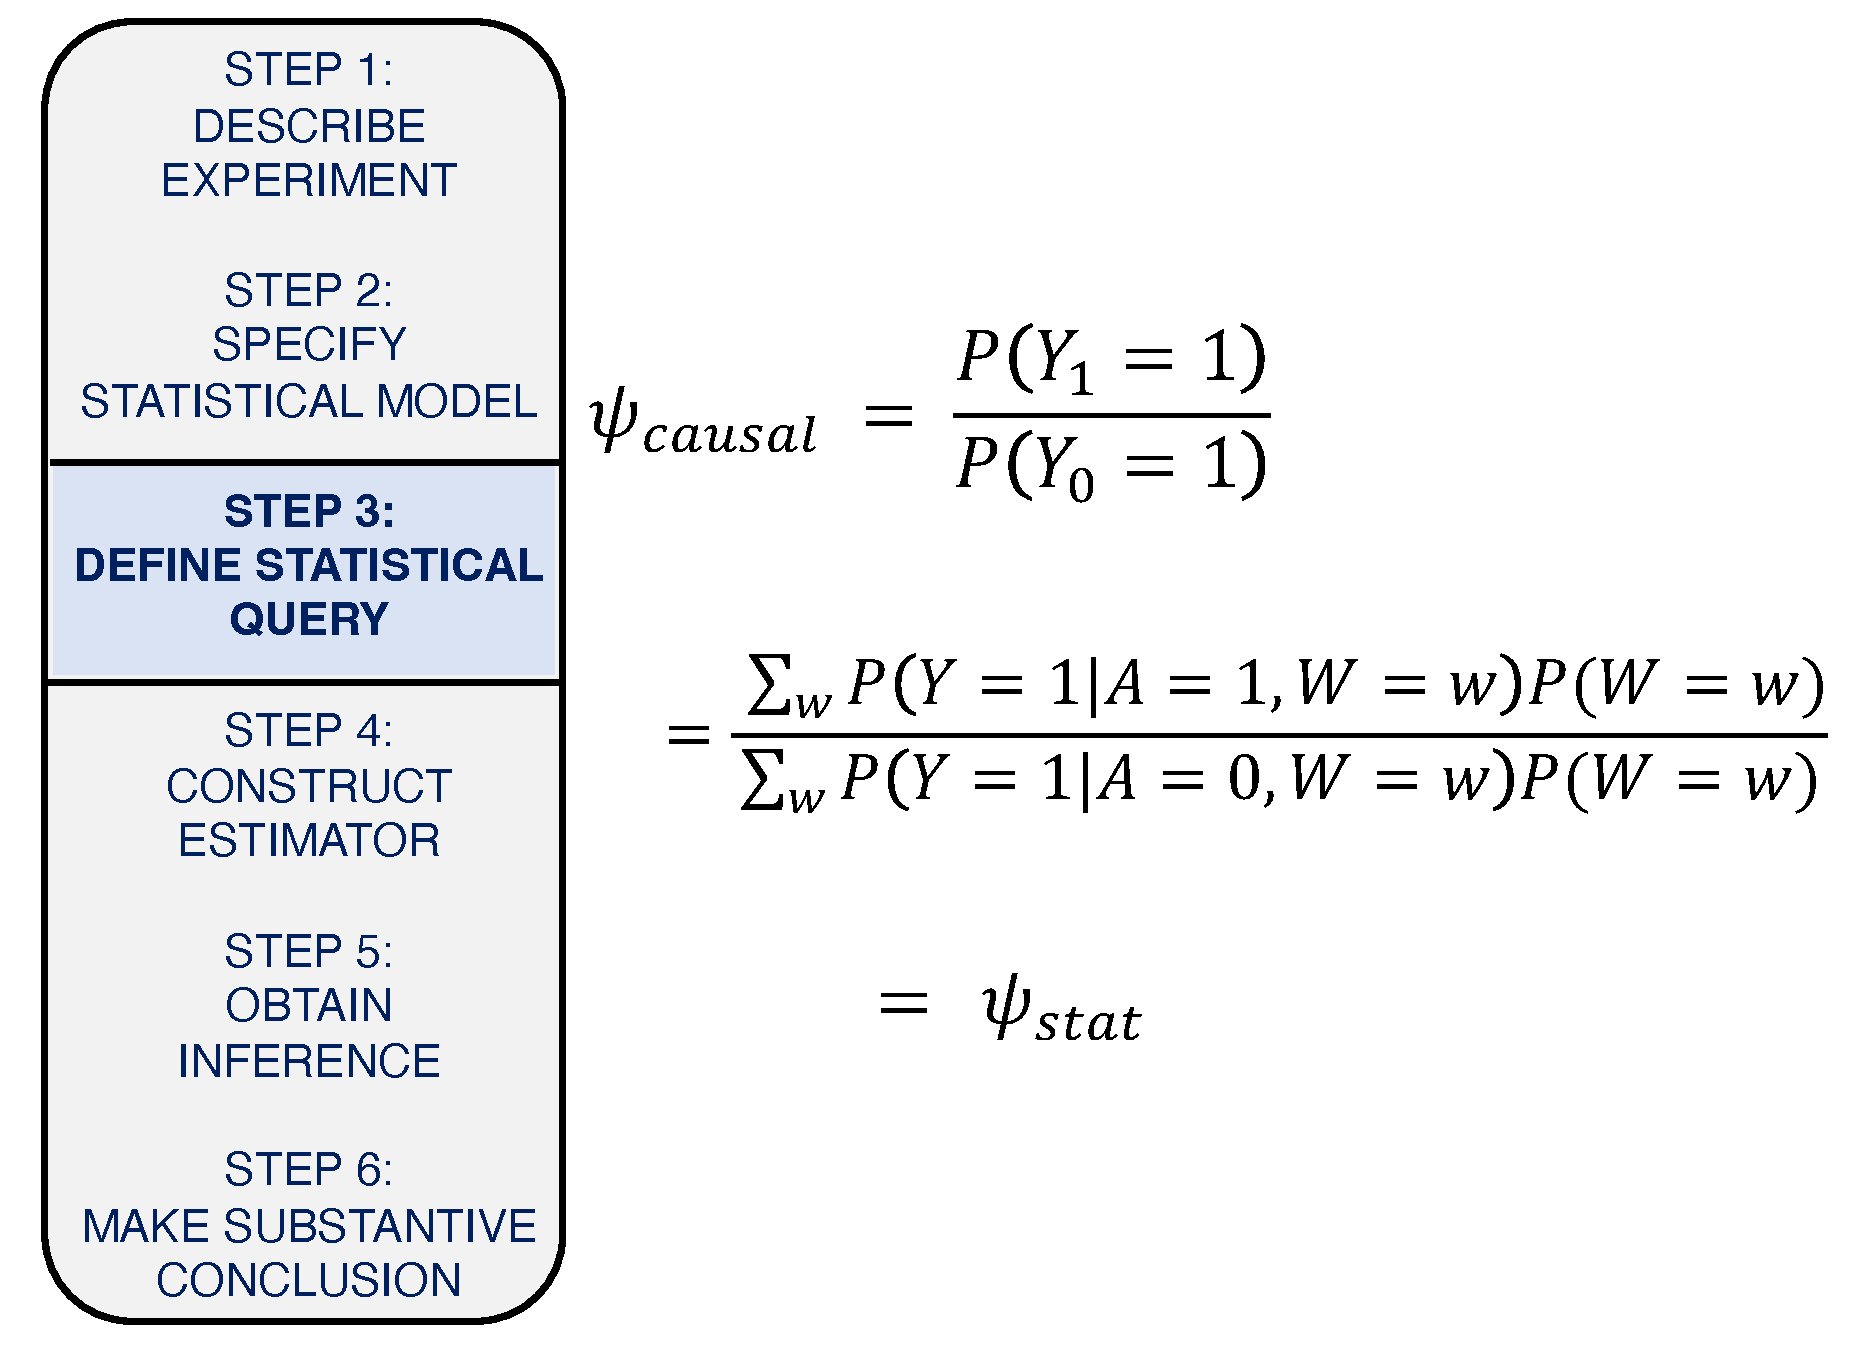
\includegraphics[width = 1.05\textwidth]{figures/Gcomp.pdf}
  \end{center}
\end{frame}

\subsubsection{Statistical estimand}
\begin{frame}
  \frametitle{Step 3b: What is the target statistical estimand that we will learn from the data?}
  \vspace{-20pt}
  \begin{center}
  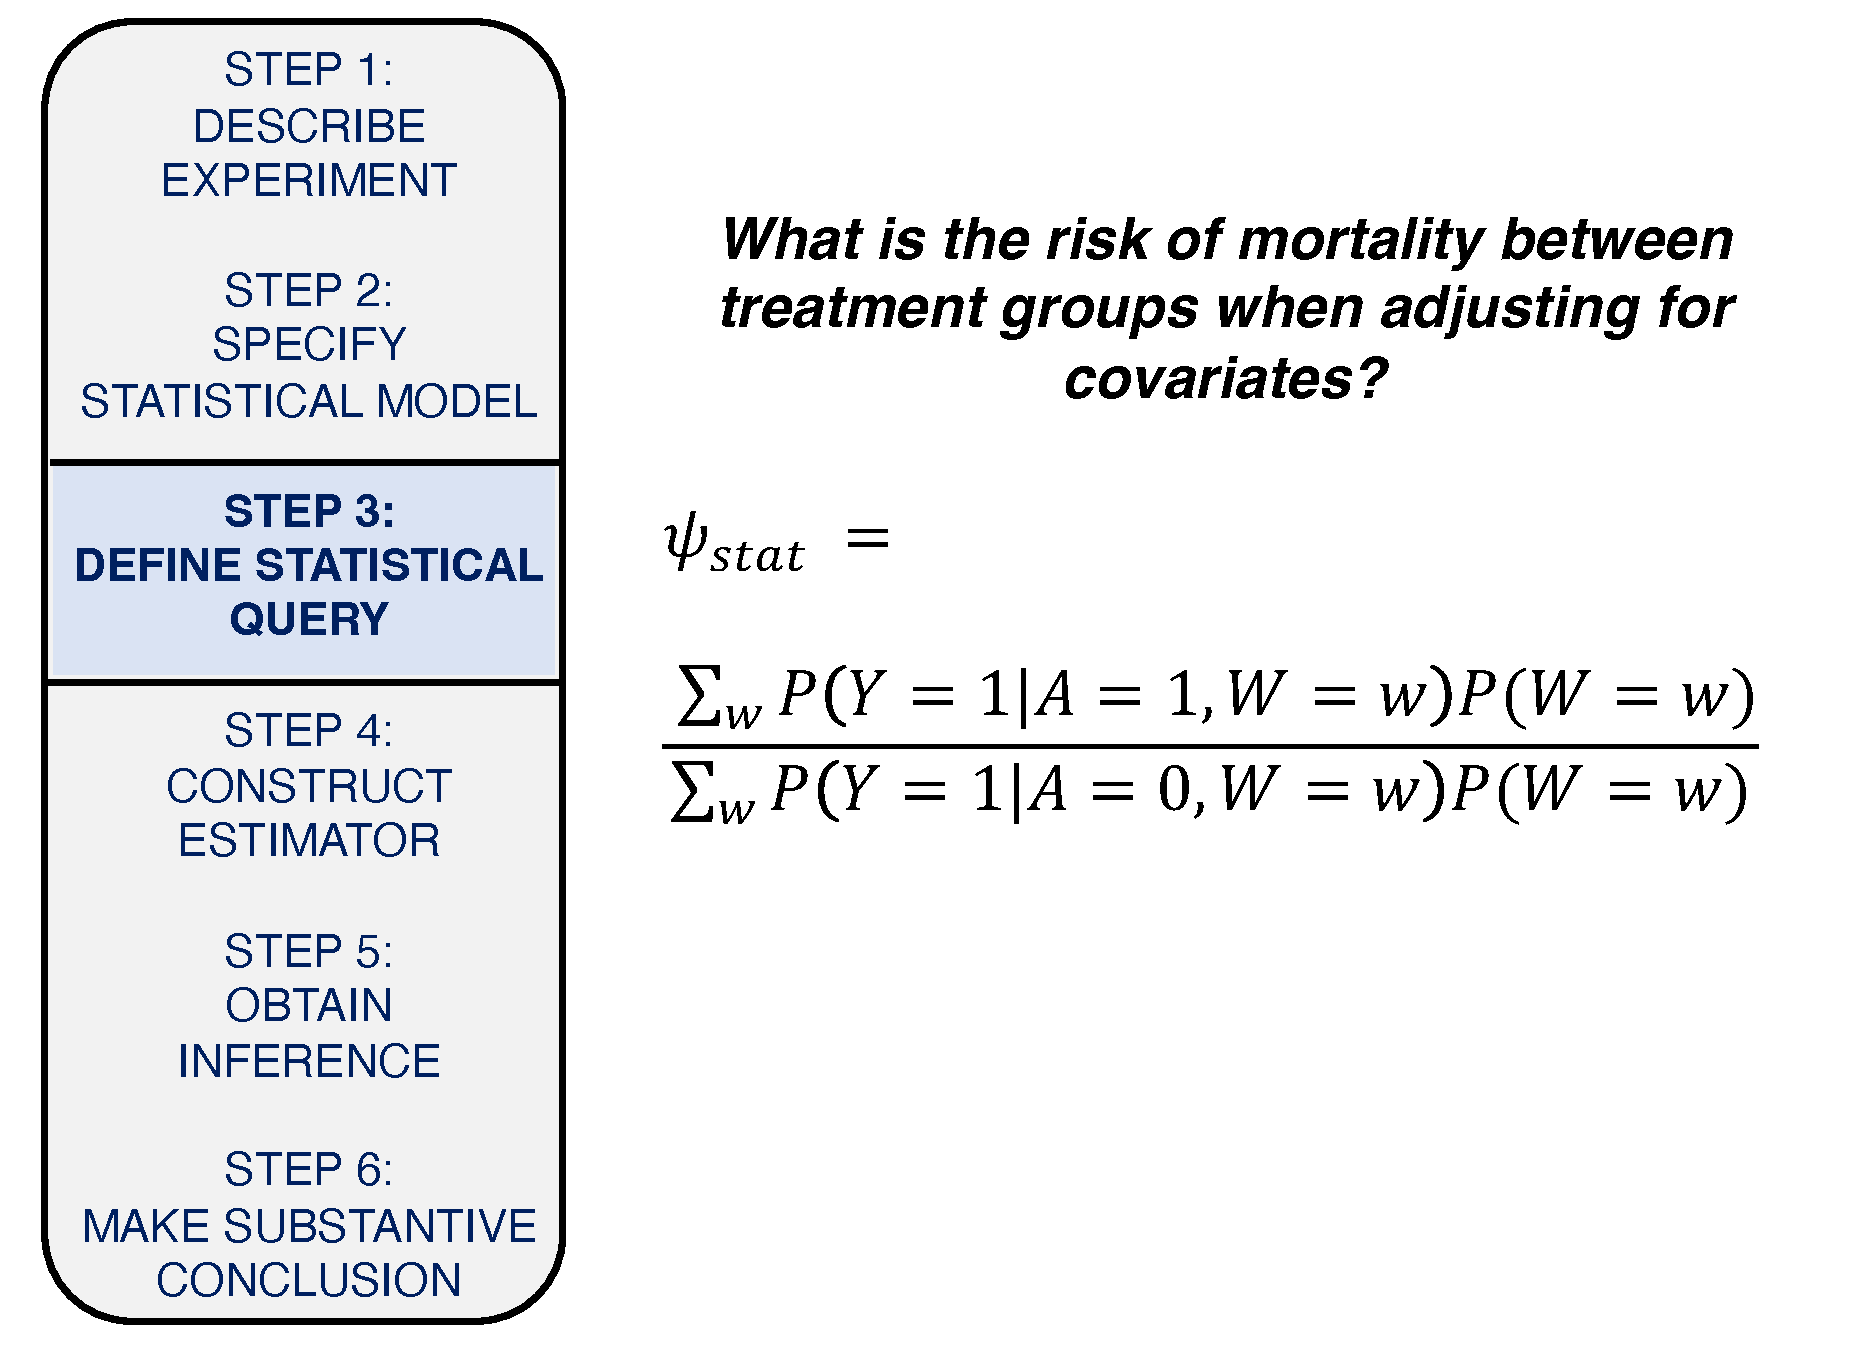
\includegraphics[width = 1.05\textwidth]{figures/stat_estimand.pdf}
  \end{center}
\end{frame}

\subsection{Construct estimator}
\begin{frame}
  \frametitle{Step 4: How should we estimate the target estimand?}
  \vspace{-20pt}
  \begin{center}
  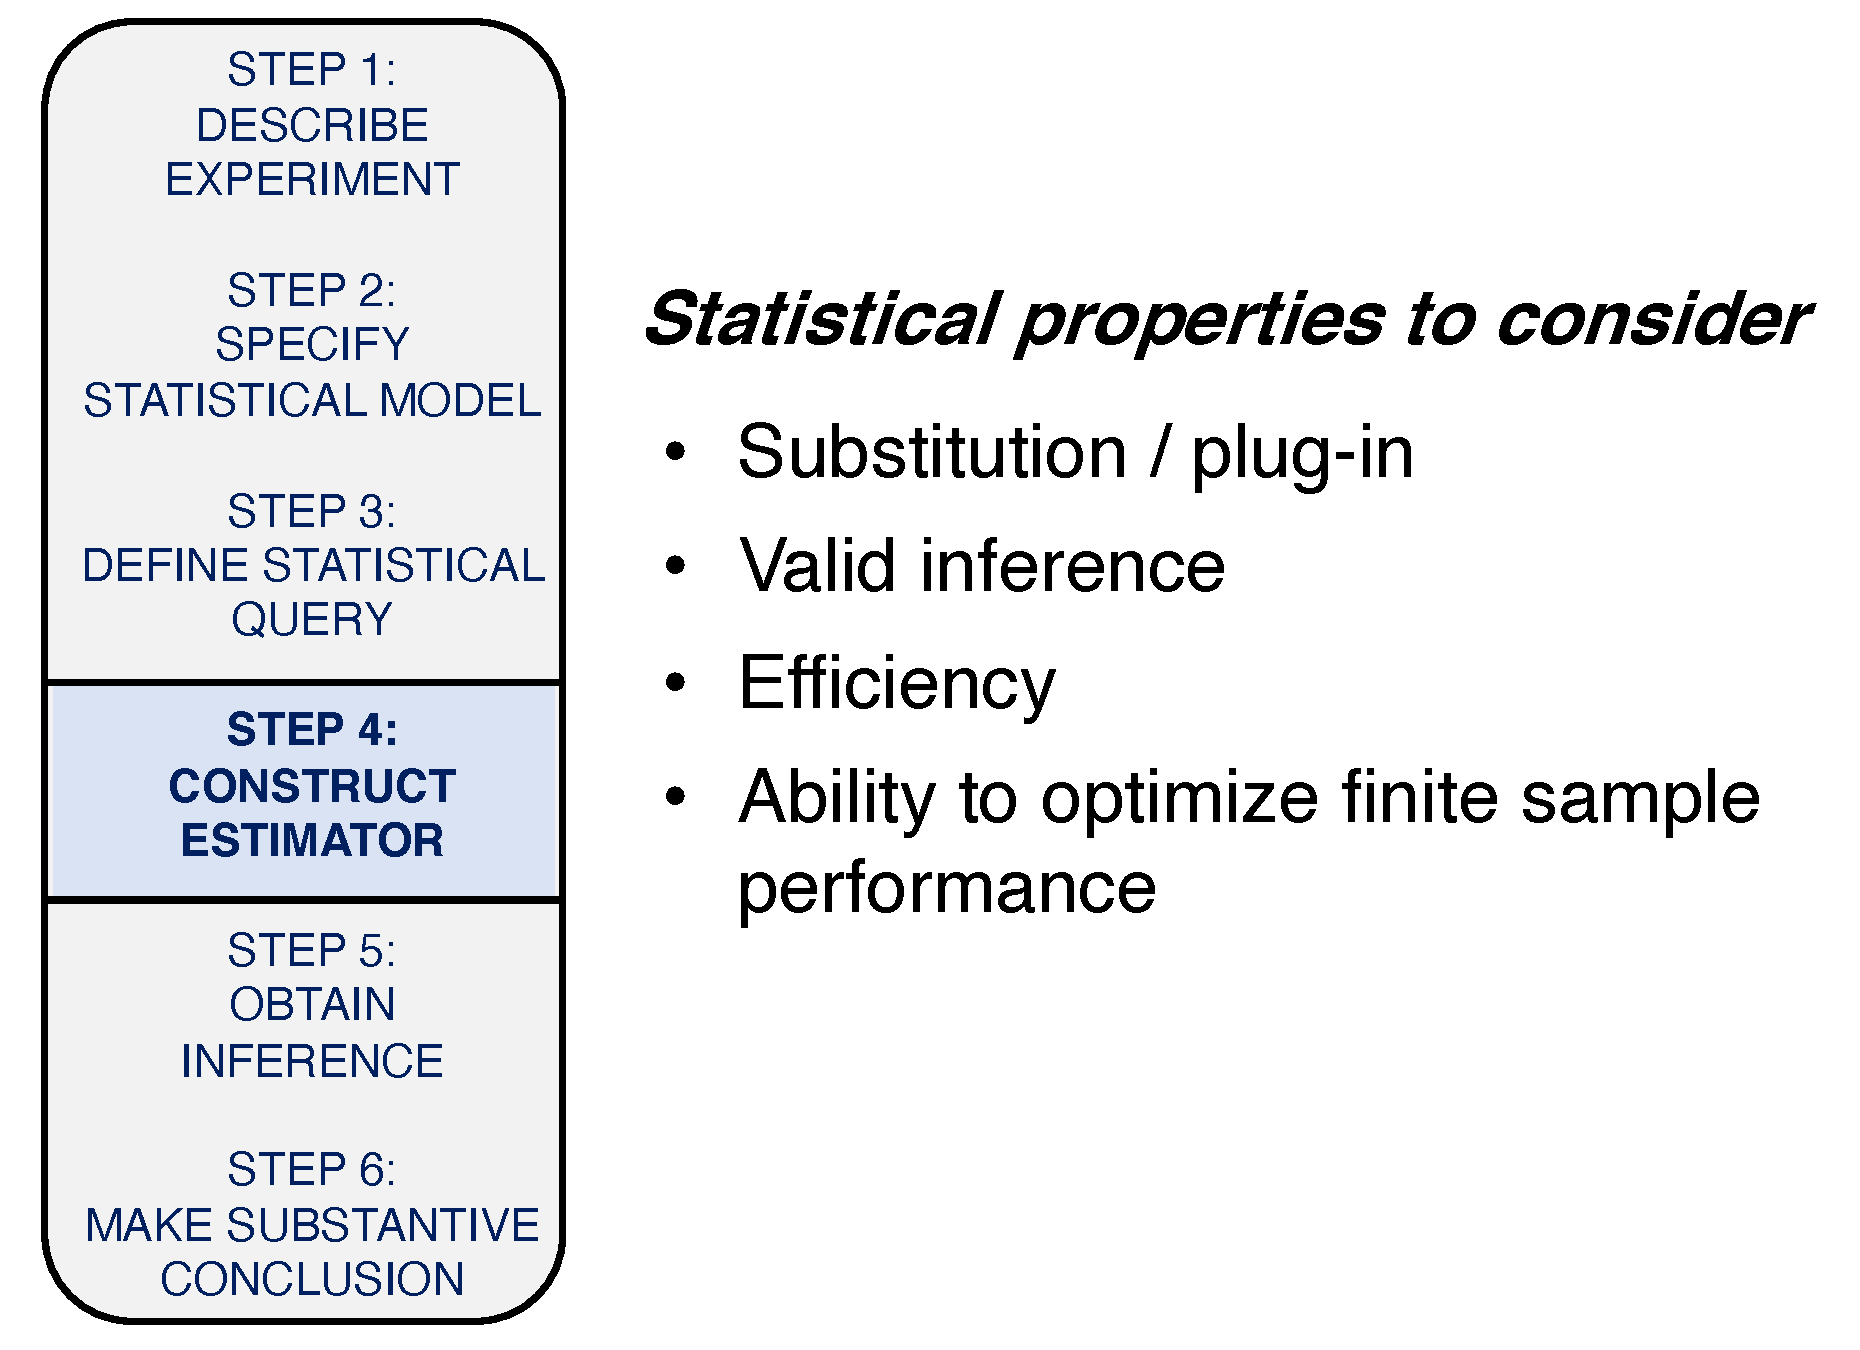
\includegraphics[width = 1.05\textwidth]{figures/roadmap4.pdf}
  \end{center}
\end{frame}

\begin{frame}
  \frametitle{Why plug-in estimation?}
  \begin{itemize}
    \item Consider a data unit $O = (W, A, Y)$, where $O \sim P_0 \in
      \mathcal{M}$ for $P_0$ the data-generating distribution in a model
      $\mathcal{M}$.
    \item A \textit{plug-in} estimator $\Psi(\hat{P}_n)$ is based on the
      parameter mapping, where the target parameter is $\Psi(P_0)$ and
      $\hat{P}_n$ is an estimator of $P_0$.
    \item $\Psi(P_0) = \mathbb{E}_0\{\mathbb{E}_0[Y \mid A = 1, W] -
      \mathbb{E}_0[Y \mid A = 0, W]\}$, the ATE functional, can be approximated
      by recognizing that:
      \begin{itemize}
        \item Components of $P_0$ that impact the plug-in estimator are the
          conditional mean $\bar{Q}_0(A,W) = \mathbb{E}[Y \mid A, W]$ and the
          marginal distribution of $W$, $Q_{0,W}$.
        \item Thus, the plug-in estimator depends on estimates of these:
          $\bar{Q}_n(A,W) = \hat{\mathbb{E}}[Y \mid A, W]$ and $Q_{n,W} =
          P_n(W = w)$.
      \end{itemize}
    \item By construction, plug-in estimators remain within the bounds of the
      parameter space.
  \end{itemize}
\end{frame}

\begin{frame}
  \frametitle{Targeted Maximum Likelihood Estimation (TMLE)}
  \vspace{-20pt}
  \begin{center}
  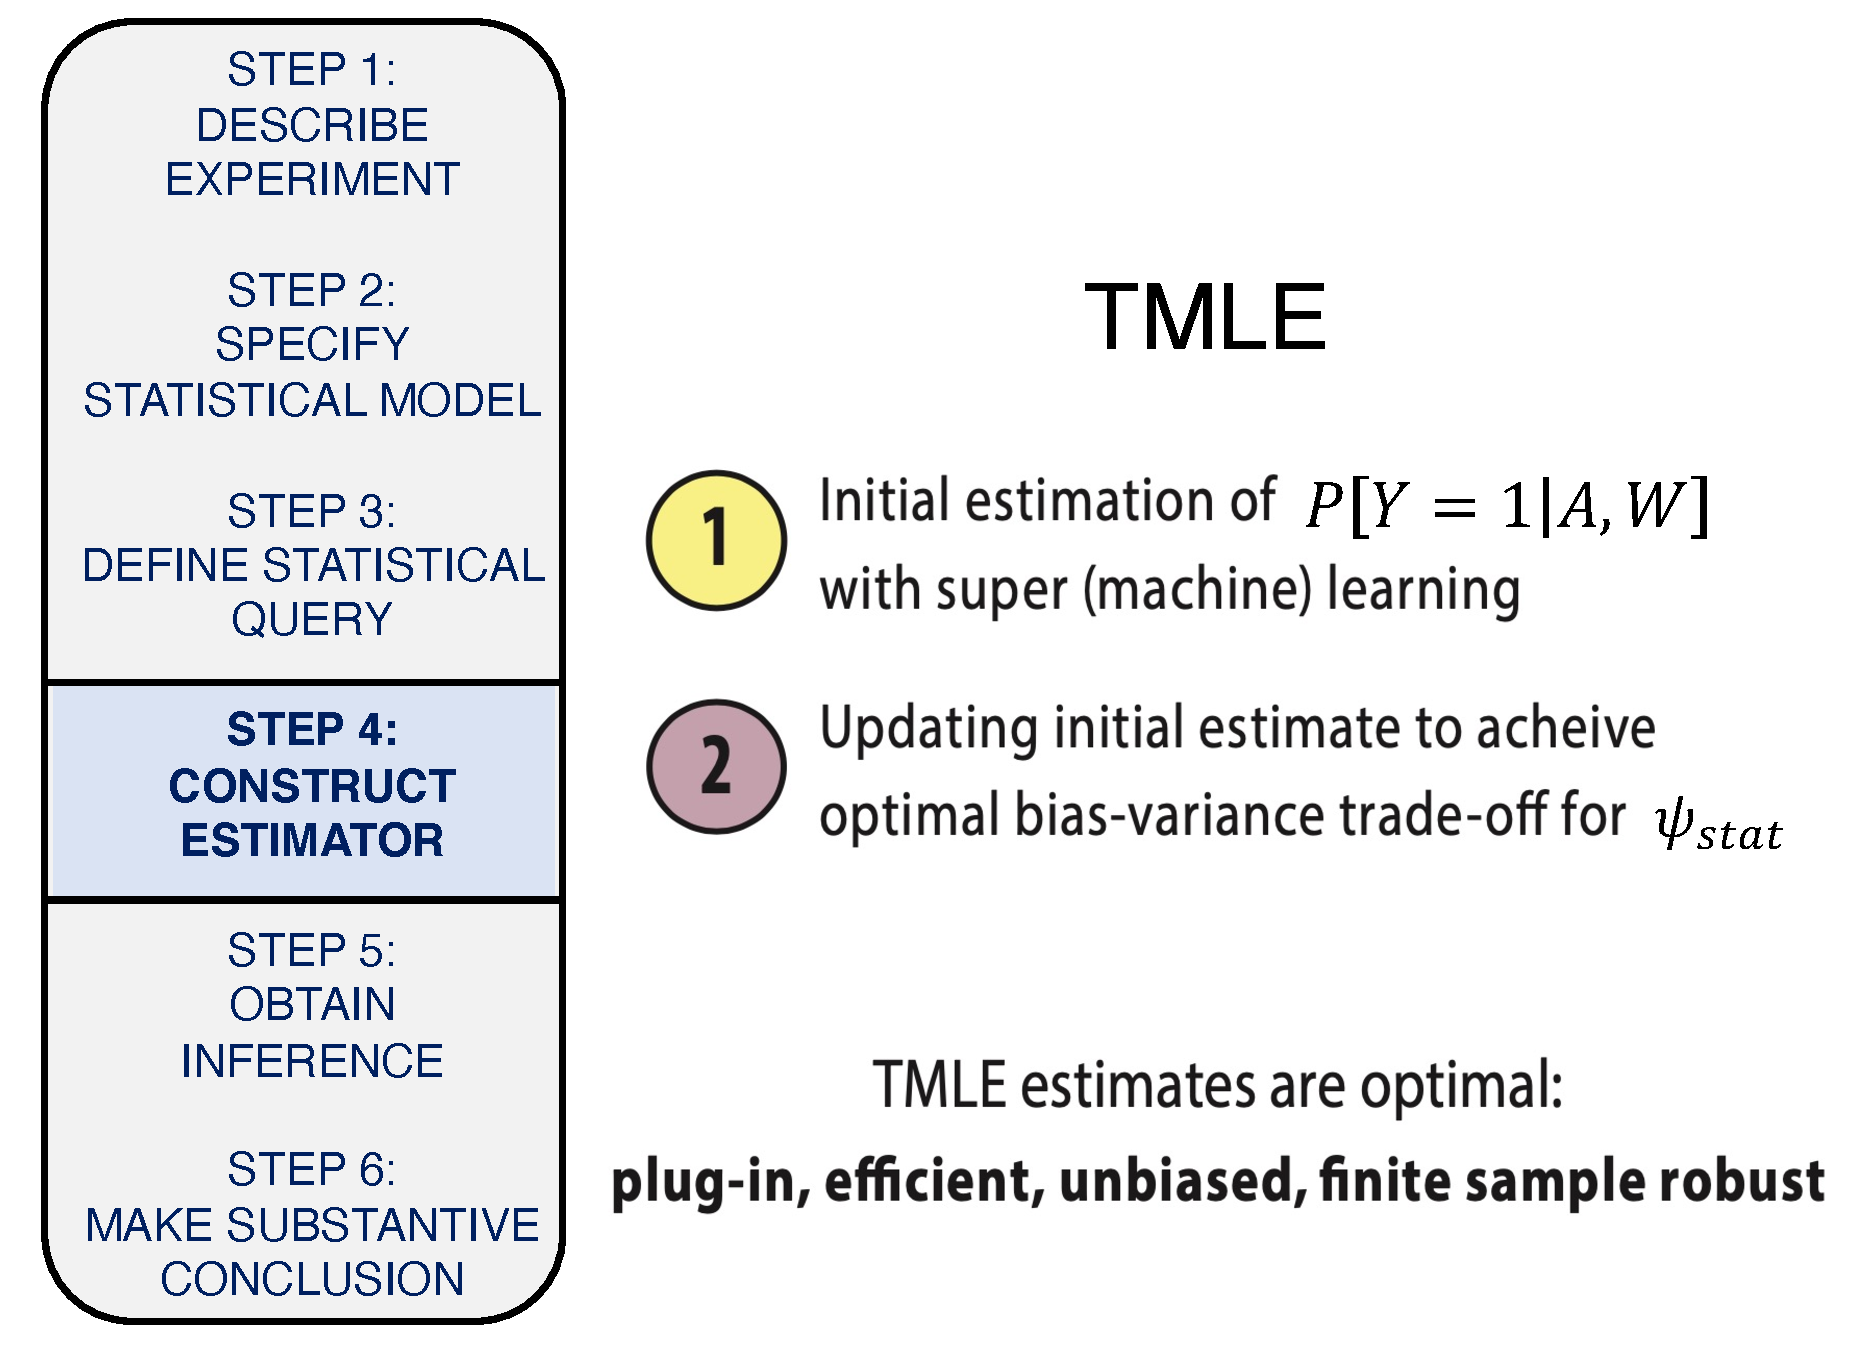
\includegraphics[width = 1.05\textwidth]{figures/tmle.pdf}
  \end{center}
\end{frame}

\begin{frame}
\frametitle{Initial estimates via super learner}
\vspace{-15pt}
\begin{center}
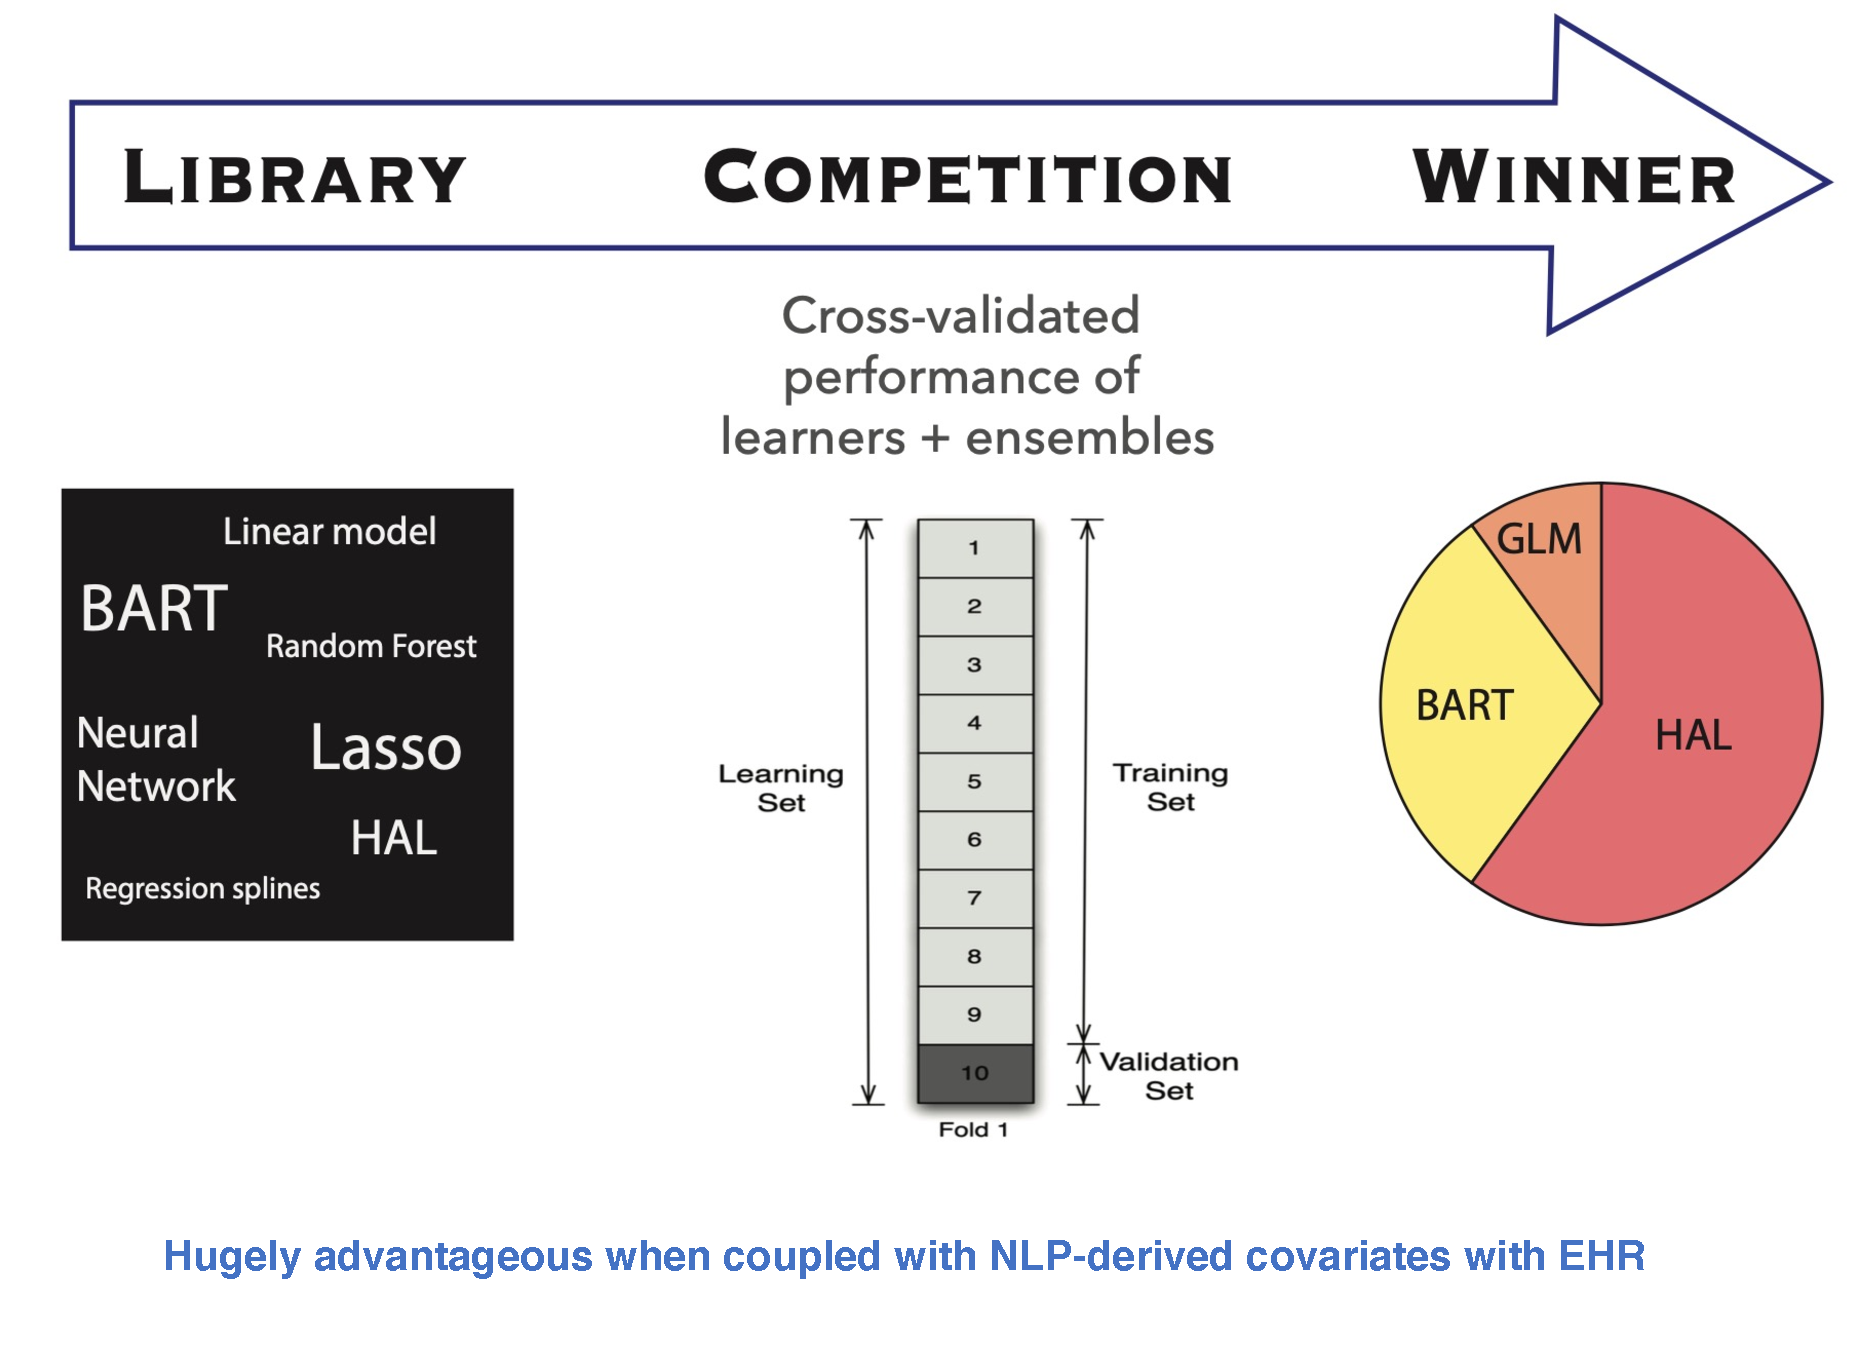
\includegraphics[width = 1\textwidth]{figures/SL.pdf}
\end{center}
\end{frame}

\begin{frame}
\frametitle{Cross-validation to choose a winner}
\vspace{-15pt}
\begin{center}
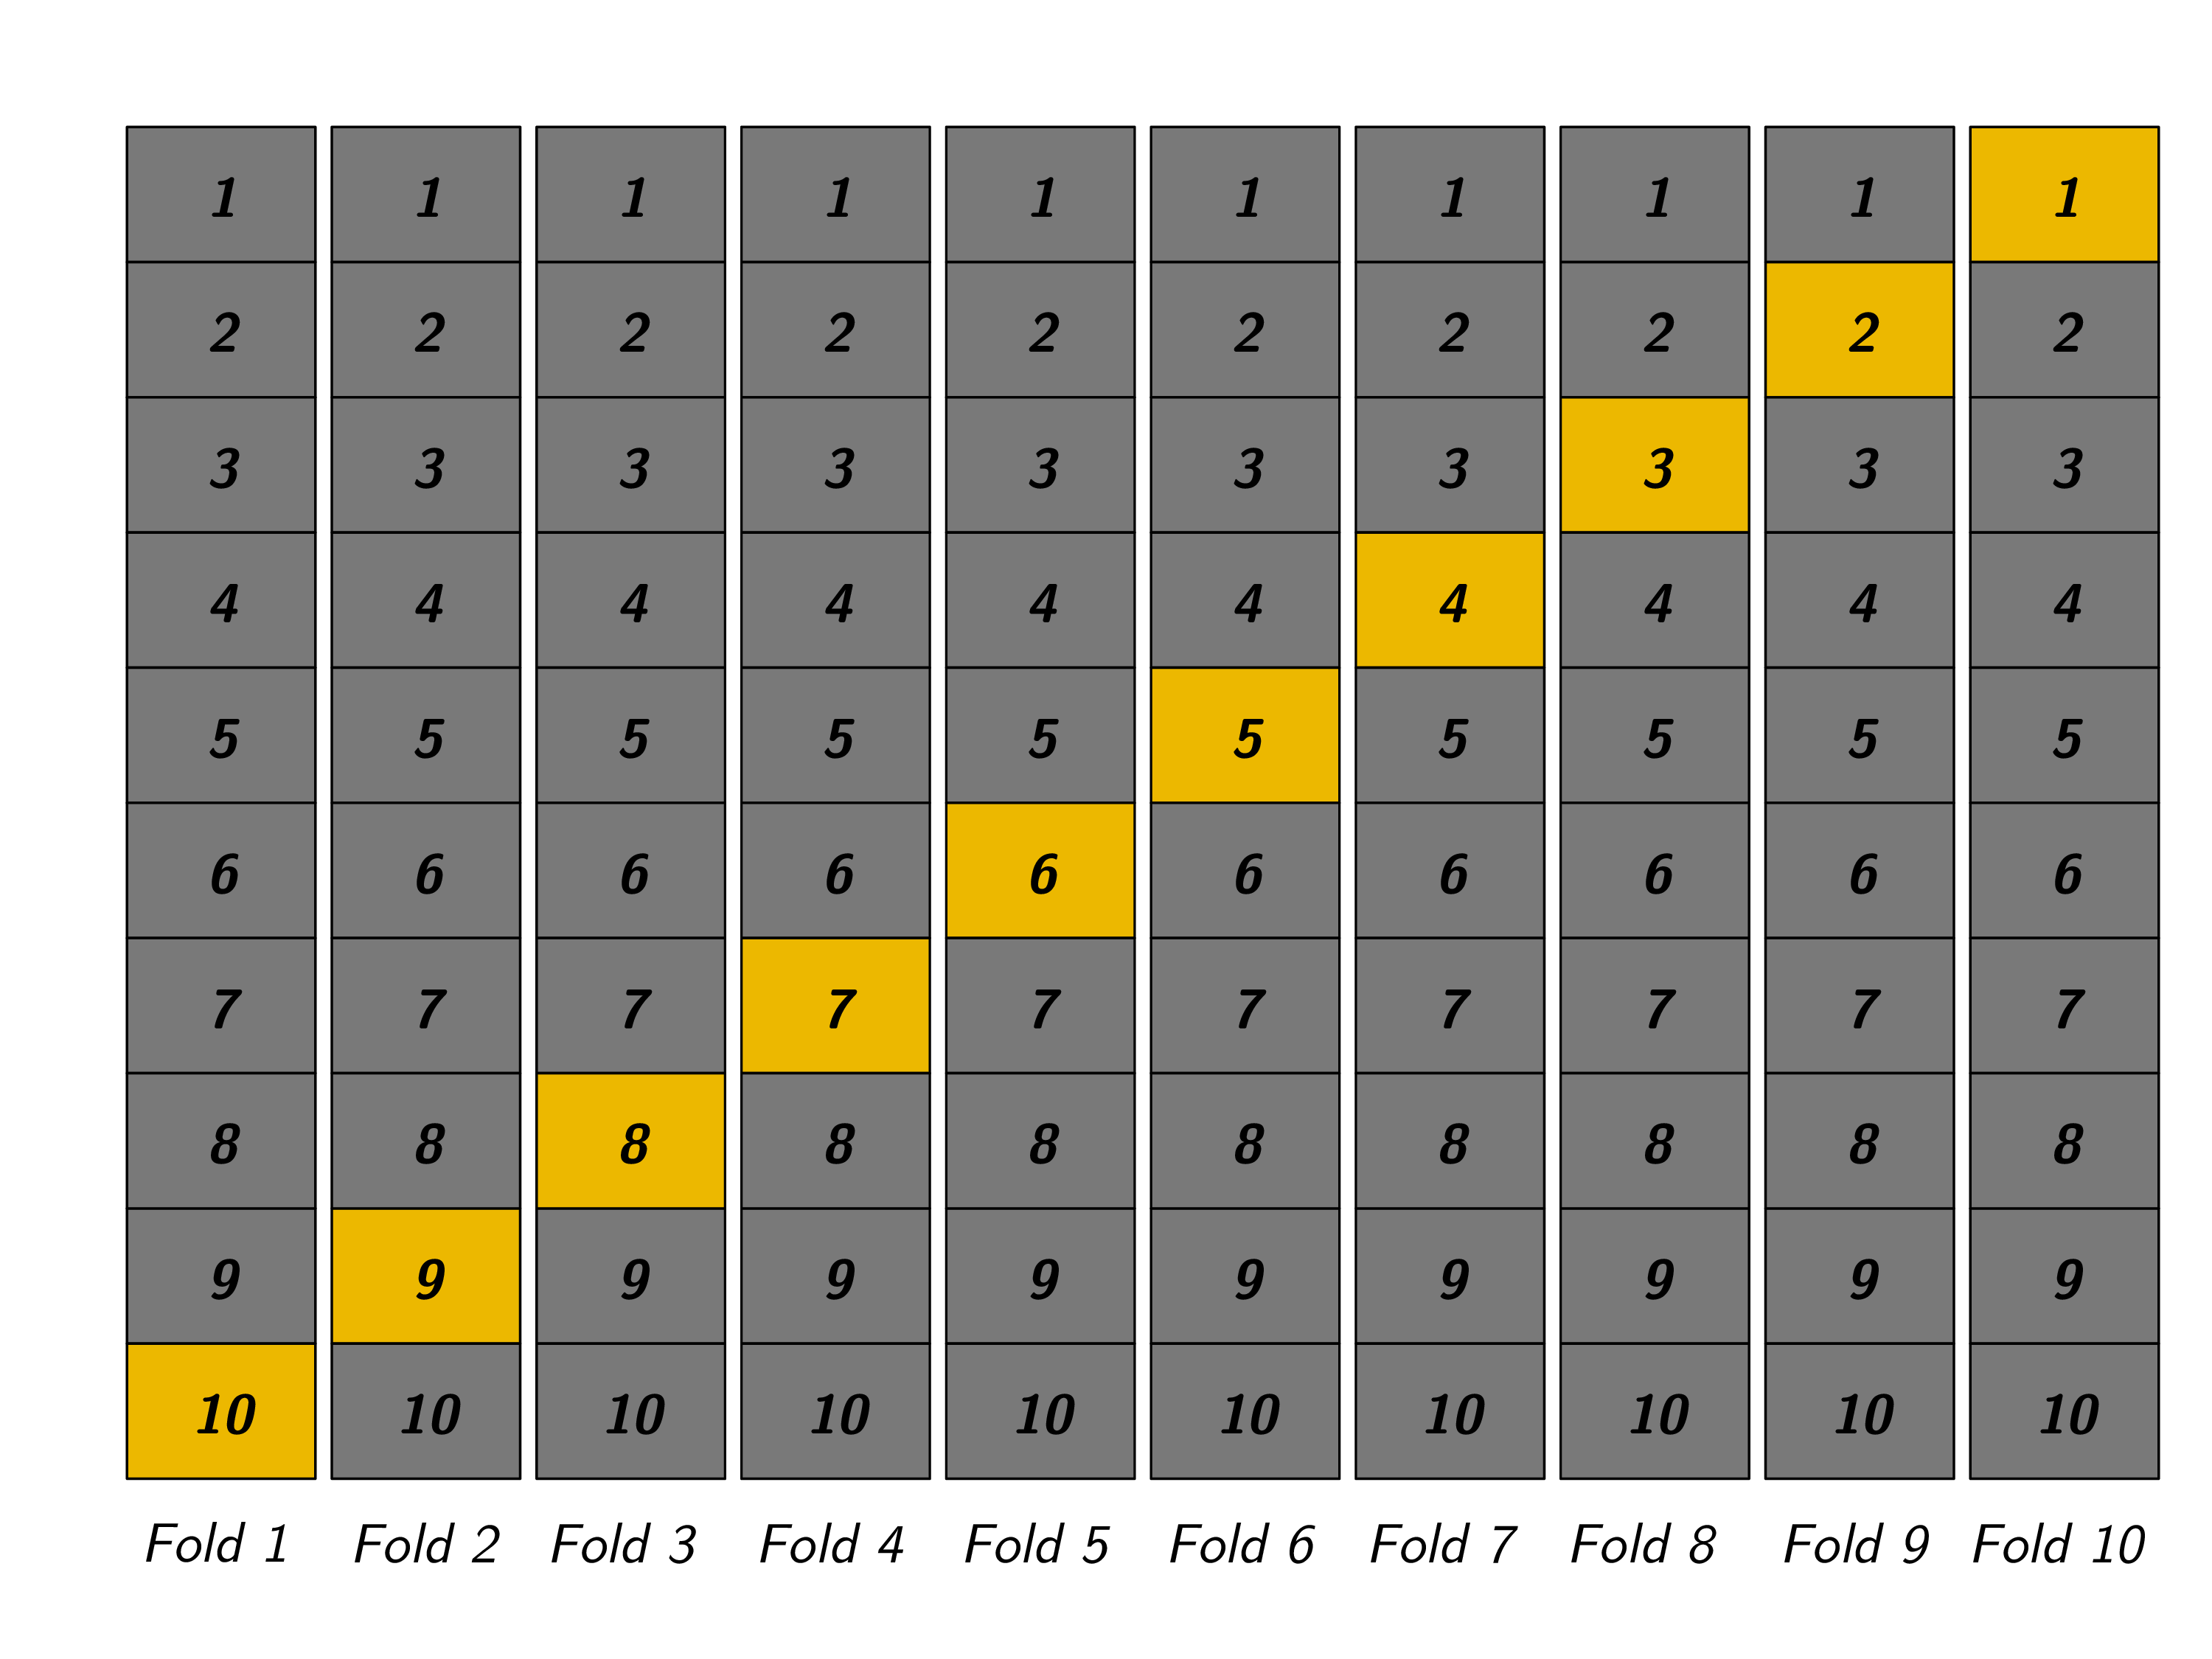
\includegraphics[width = 1\textwidth]{figures/vs.png}
\end{center}
\end{frame}

\begin{frame}
  \frametitle{Coding exercise: Super learning with \texttt{sl3}}
  \url{https://tlverse.org/catalyst2024-workshop/sl3.html}
\end{frame}

% \begin{frame}
% \frametitle{Tip: Include the Highly Adaptive Lasso (HAL) as a candidate in the SL library}
% \begin{itemize}
%      \item HAL converges to true function at rate $n^{-1/3}(\log n)^{d/2}$
%     \item It is the first estimator that guarantees asymptotically efficient estimation of any pathwise differentiable estimand\footnote{An estimand that is a weakly differentiable functional of the density of the data, the case for most causal inference estimands under positivity.} (e.g., the average causal effect or treatment-specific survival), without enforcing strong smoothness conditions
%     \item Assumptions are exceedingly mild, and expected to hold in almost every practical application
%     \item Software for HAL is available in the \texttt{tlverse}, see the \texttt{hal9001} package on CRAN, and it can be used in standard SL sofware (\texttt{SuperLearner} and \texttt{sl3})
%     \item HAL is interpretable
%     % \item Can be implemented for a large variety of function spaces, whose choice can be selected with cross-validation.
% \end{itemize}
% \end{frame}

\begin{frame}
\frametitle{Tip: Include the Highly Adaptive Lasso (HAL) as a candidate in the SL library}
\begin{itemize}
    \item First estimator to guarantee asymptotically efficient estimation of
      any pathwise differentiable estimand\footnote{An estimand that is a weakly
      differentiable functional of the density of the data, the case for most
      causal inference estimands under positivity.} (e.g., average causal effect
      or treatment-specific survival), without enforcing local smoothness
      conditions.
    \item Mild assumptions, which hold in most practical applications.
    \item Regularization step can be implemented with standard Lasso software
      (e.g., \texttt{glmnet}).
    \item Converges to true function at rate $n^{-1/3}(\log n)^{d/2}$.
    \item Accommodates a variety of function space specifications.
    % \item Can be implemented for a large variety of function spaces, whose choice can be selected with cross-validation.
\end{itemize}
\end{frame}

\begin{frame}
\frametitle{Illustration in Low Dimensions}
\vspace{-5pt}
\begin{center}
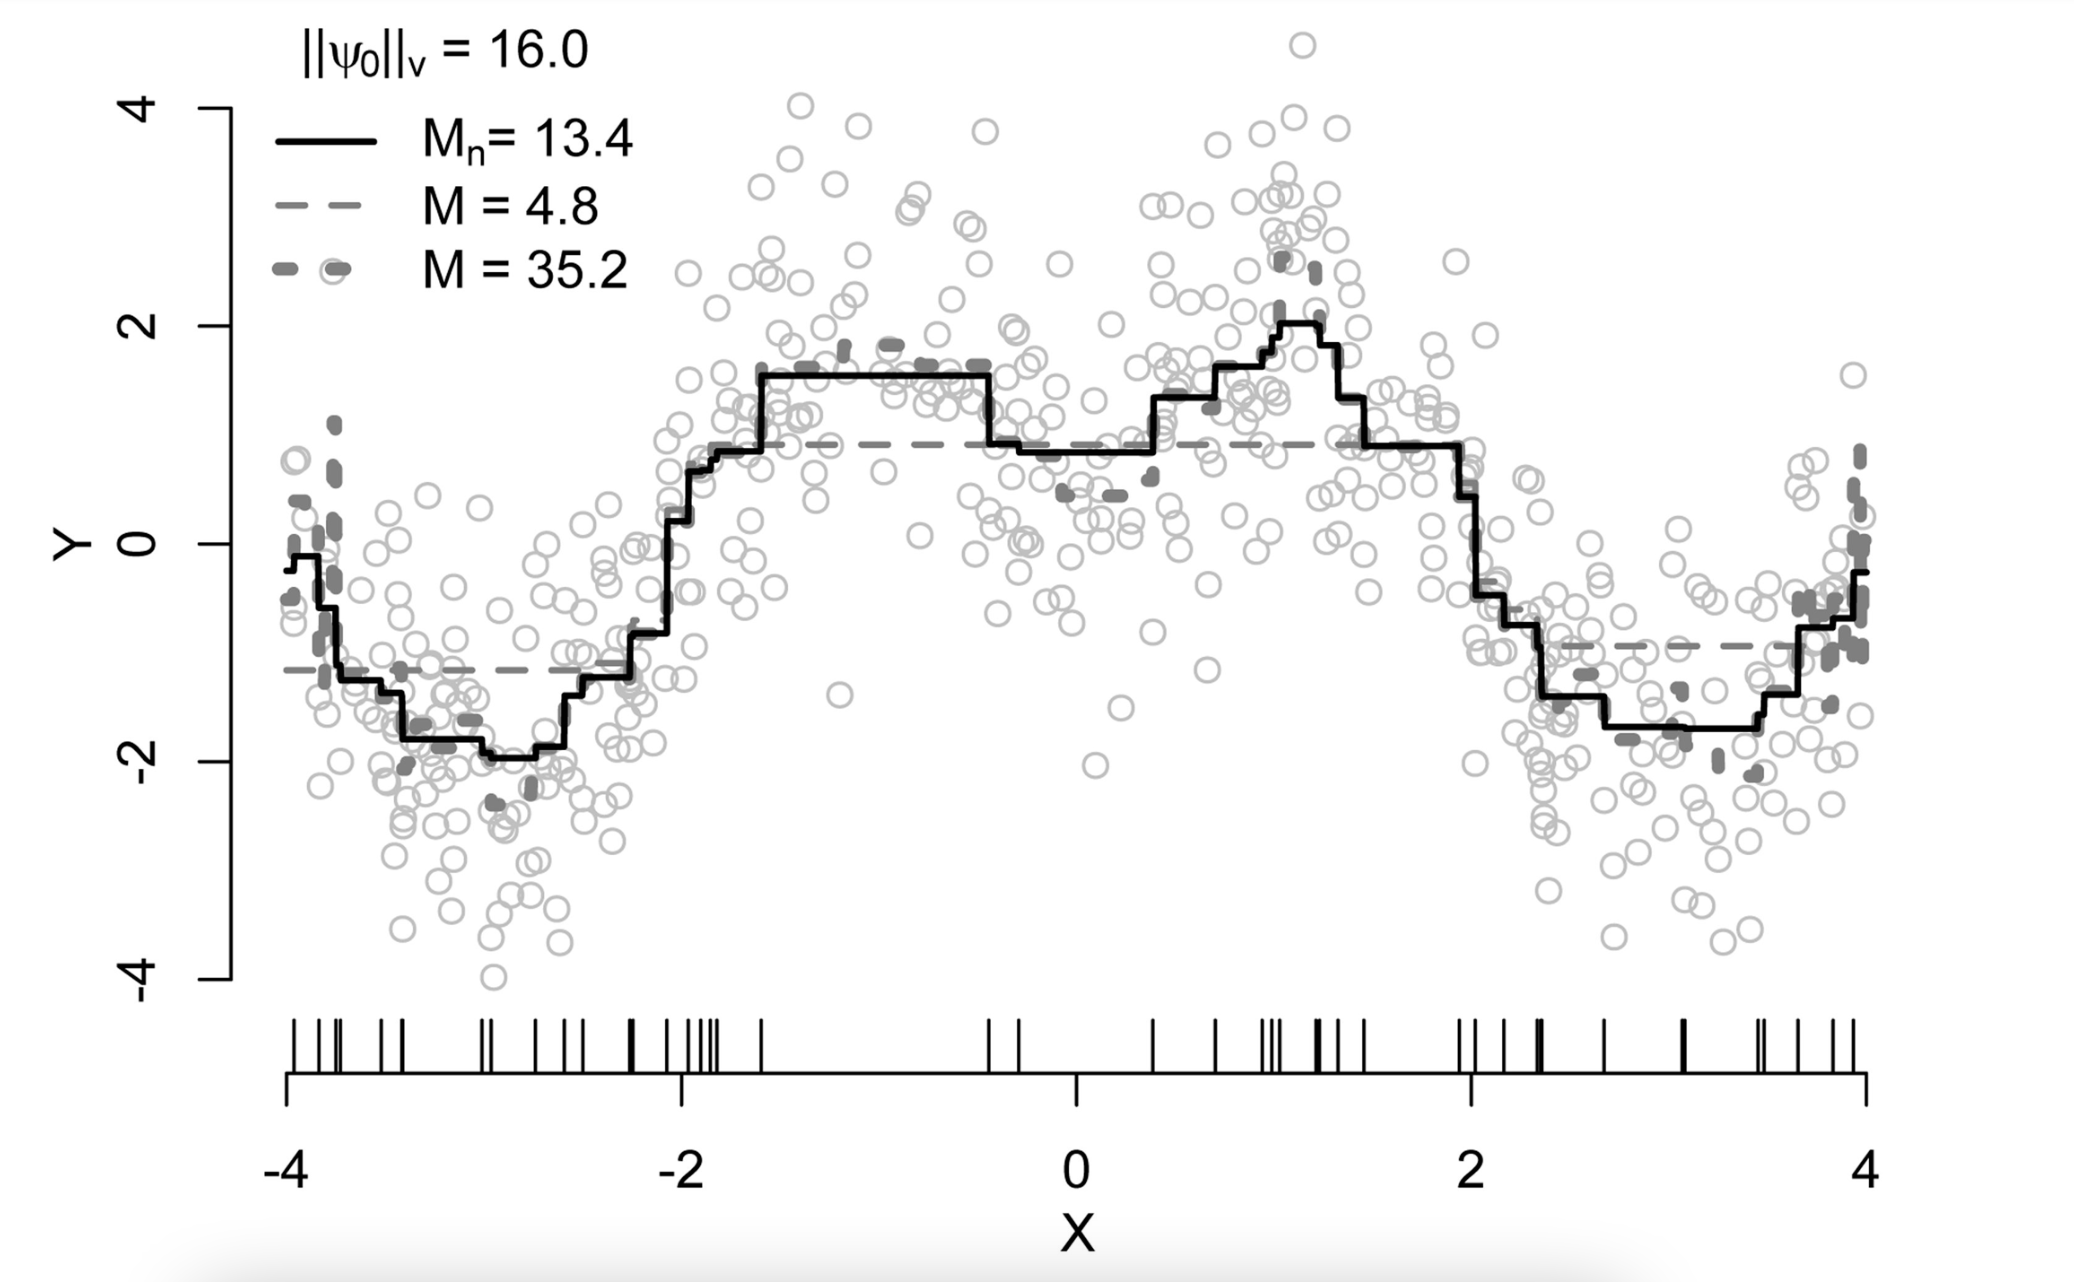
\includegraphics[width=1.1\textwidth]{figures/HAL-univariate.png}
\end{center}
% For the univariate setting, we drew n = 500 independent copies of X from a Uniform(-4,4) and of ε from a Normal(0, 1) distribution and let Y = 2sin(π/2|X|) + ε, so that ‖ψ0‖υ = 16. The basis functions used by the HAL estimator consist of n indicators at the observed data points: φj(x) = I(x ≥ x̃j) for j = 1, ..., n. To select the bound on the variation norm, we used ten-fold cross validation to select from 100 possible bounds ranging from 0 to about 350. We illustrate the fit from three of these choices in Figure. The solid line is the HAL estimator, which uses the cross-validation-selected value Mn = 13.9. The dashed and dotted lines represent choices that are smaller and larger than the true variation norm, respectively. The ticks at the bottom of the figure are placed at the 46 support points of ψn with a non-zero coefficient. The choice of 4.8 as bound on the variation norm (dashed line) visibly over-smooths the data, while the bound of 35.2 appears to provide a reasonable approximation and is similar with the prediction from the HAL estimator. However, the larger bound does appear to produce more noise near the edges of the support. Theory dictates that any choice of bound larger than the true norm will yield an estimator with the properties established in Theorem 1. Nevertheless, we expect that the HAL estimator will exhibit superior performance in finite samples by allowing for selection of a bound smaller than the true norm. The oracle inequality guarantees that so long as at least one bound larger than the true norm is considered as a candidate bound, then we will eventually select a bound that is larger than the true variation norm. Indeed, when the sample size was increased to 5,000 (data not shown), the cross-validation-selected bound was selected as 16.8, which is close to the true value.
\end{frame}

%\begin{frame}
  %\frametitle{Coding exercise: Highly adaptive lasso with \texttt{hal9001}}
%\end{frame}

% \begin{frame}
% \frametitle{Basic \texttt{R} \texttt{hal9001} Functionality}
% \begin{enumerate}
%     \item Load package and data: \newline \texttt{library(hal9001)} \newline
%     \texttt{data(mtcars)}
%     \item Create numeric vector for dependent variable: \newline \texttt{Y <-  mtcars[,"mpg"]}
%     \item Create dataframe or matrix of predictors: \newline
%     \texttt{X <- mtcars[,c("cyl", "disp", "hp", "wt")]}
%     \item Fit HAL: \newline
%    \texttt{ hal\_fit <- fit\_hal(X=X, Y=Y)}\newline
%    \newline
%    \small{\textit{Note}: default arguments \texttt{max\_degree=3} considers no more than 3-way interactions, and default \texttt{reduce\_basis=0} places no restrictions on the minimum proportion of 1's in basis functions.}
% \end{enumerate}
% \end{frame}

% \begin{frame}
% \frametitle{Summary table of \texttt{hal9001}  HAL fit}
% \vspace{-2pt}
% \texttt{summary(hal\_fit)\$table}
% \begin{center}
% \vspace{-2pt}
% 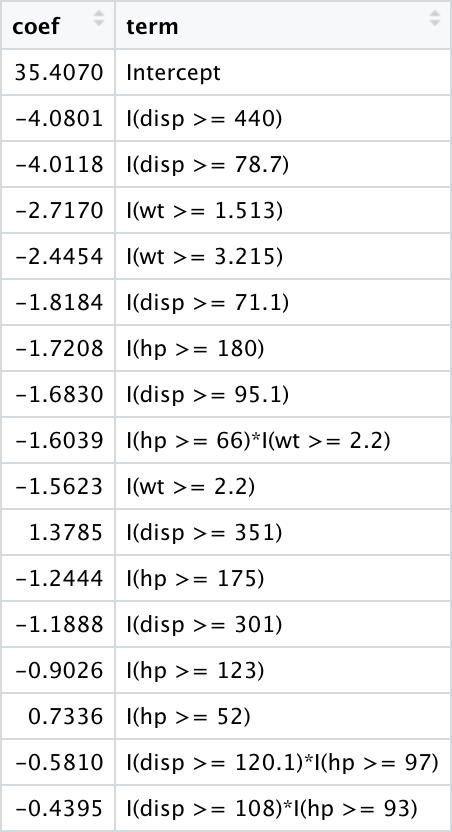
\includegraphics[width = 0.38\textwidth]{figures/HAL-summary-mtcars.png}
% \end{center}
% \end{frame}

% \begin{frame}
% \frametitle{Overview of HAL}
% {\bf A maximum likelihood estimator over all, or subset of, cadlag functions with finite variation norm.}
% \begin{block}{\large{Key Ingredients}}
% \begin{itemize}
% \item Any stochastic relation/function we aim to learn from data can be approximated by linear combination (i.e., sum) of spline basis functions $X\rightarrow I(X>x_j)$ for knot point $x_j$.
% \item The variation norm (i.e., complexity) of a function is the $L_1$-norm.
% \item Optimize empirical performance over all such linear models under fixed $L_1$-norm that is selected with cross-validation.
% %\item Optimize empirical performance over all such linear models under fixed $L_1$-norm.
% %\item The $L_1$-norm is optimally selected with cross-validation.
% \vspace{.1in}
% \end{itemize}
% \end{block}

% \blfootnote{van der Laan, Mark. "A generally efficient targeted minimum loss based estimator based on the highly adaptive lasso." The International Journal of Biostatistics (2017).}
% \end{frame}

% \begin{frame}
% \frametitle{HAL is theoretically proven to approximate truth faster than known machine learning algorithms}
% \vspace{-5pt}
% \begin{center}
% 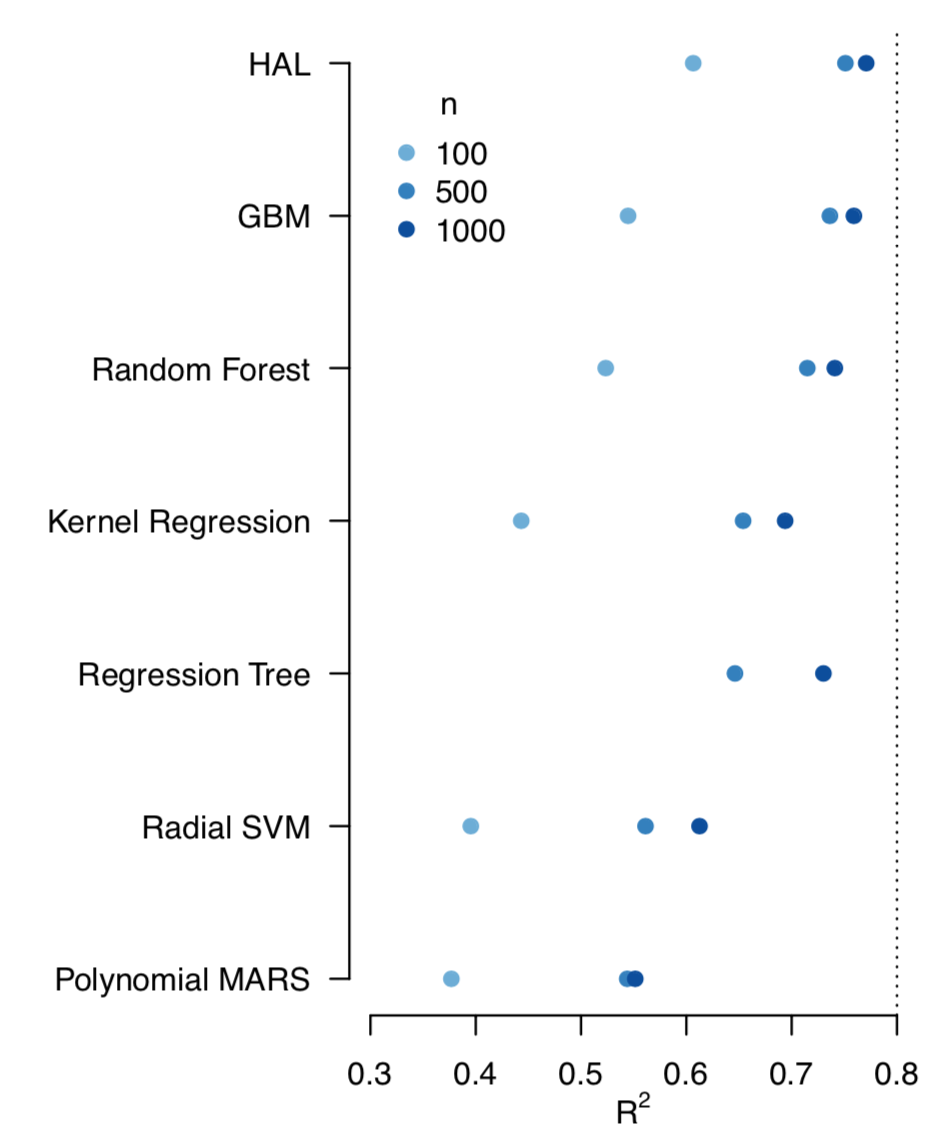
\includegraphics[width=.6\textwidth]{figures/HAL-works.png}
% \end{center}
% \end{frame}

\subsection{Obtain inference}

\begin{frame}
\frametitle{TMLE: Targeting by following a path of maximal change in target estimand per unit likelihood}
\vspace{-13pt}
\centering
\begin{figure}
\centering
\animategraphics[autoplay,loop,width=0.92\linewidth]{7}{figures/ULFS_n400/gganim_plot}{0001}{0100}
\end{figure}
\end{frame}

\begin{frame}
  \frametitle{TMLE Example for the ATE functional}
  \begin{itemize}
    \item Consider again $O = (W, A, Y)$ where $O \sim P_0 \in \mathcal{M}$.
    \item $\Psi(P_0) = \mathbb{E}\{\mathbb{E}[Y \mid A = 1, W] - \mathbb{E}[Y
      \mid A = 0, W]\}$, the ATE functional, has a plug-in estimator:
      $$\Psi(Q_n) = \frac{1}{n}\sum_{i=1}^n\{\bar{Q}_n(1, W) - \bar{Q}_n(0,
      W)\} \ ,$$ where $\bar{Q}_n(a, W) = \hat{\mathbb{E}}[Y \mid A = a, W]$.
    \item The TMLE based on this plug-in estimator is
      $$\Psi(Q_n^{\star}) = \frac{1}{n}\sum_{i=1}^n\{\bar{Q}_n^{\star}(1, W) -
        \bar{Q}_n^{\star}(0, W)\} \ ,$$ where $\bar{Q}_n^{\star}$ is an update
        of the initial estimate $\bar{Q}_n(a, W)$
    \item The update step uses a parametric fluctuation of the form
      $\text{logit}(\bar{Q}_n^{\star}) = \text{logit}(\bar{Q}_n) + \epsilon
      H_n(A,W),$ where the form of $H_n(A,W)$ depends on relevant efficiency
      theory.
  \end{itemize}
\end{frame}

\begin{frame}
  \frametitle{TMLE Example for the ATE functional}
  \begin{itemize}
    \itemsep4pt
    \item The update step uses a parametric fluctuation of the form
      $\text{logit}(\bar{Q}_n^{\star}) = \text{logit}(\bar{Q}_n) + \epsilon
      H_n(A,W)$
    \item $H_n(A,W) = \{I(A = 1) / g_n(W)\} - \{I(A = 0) / (1 - g_n(W))\}$,
      a weight in the efficient influence function (EIF) of regular
      asymptotically linear (RAL) estimators of $\Psi(P_0)$ wrt $\mathcal{M}$.
    \item $\epsilon_n$ is a maximum likelihood estimator of $\epsilon$, so that
      the TMLE is $\Psi(P_n^{\star})$, where $P_n^{\star} = P_n^0(\epsilon_n)$.
  \end{itemize}
\end{frame}

\begin{frame}{Analysis of TMLE (vdL, Rubin, 2006)}
\begin{itemize}
\item Construct initial estimator ${\bf P}_n$; determine a least favorable path
  $\{{\bf P}_{n,\epsilon}:\epsilon\in (-\delta,\delta)\}\subset {\cal M}$
  through ${\bf P}_n$ with score $D^*_{{\bf P}_n}$ at $\epsilon = 0$.
\item Compute MLE $\epsilon_n =\arg\max_{\epsilon}P_n L({\bf P}_{n,\epsilon})$,
  where $L(P)$ is a valid loss function so that $\Psi(\arg\min_P
  P_0L(P))=\Psi(P_0)$.
\item Let ${\bf P}_n^*={\bf P}_{n,\epsilon_n}$. The TMLE is given by $\Psi({\bf
  P}_n^*)$.
\item If the mapping $\Psi(\cdot)$ is pathwise differentiable,
  $\Psi({\bf P}_n^*)-\Psi(P_0)=(P_n-P_0)D^*_{{\bf P}_n^*}+R({\bf P}_n^*,P_0)$,
  with $R(P,P_0)\equiv \Psi(P)-\Psi(P_0)-(P-P_0)D^*_P$ an exact second-order
  remainder; assume $R(P_n^*,P_0) = o_P(n^{-1/2})$.
\item Use super learner to obtain initial estimator ${\bf P}_n$, then the TMLE
  $\Psi({\bf P}_n^*)$ will be an asymptotically efficient estimator of
  $\Psi(P_0)$ under regularity conditions.
\end{itemize}
\end{frame}

\begin{frame}
  \frametitle{Asymptotic Linearity of the TMLE}
  \begin{itemize}
    \item The TMLE $\Psi(P_n^{\star})$ is a RAL estimator, from which it follows
      that its difference from $\Psi(P_0)$, the truth, can be approximated by
      an average of i.i.d.~RVs, the EIF, of $O$:
      $$\Psi(P_n^{\star}) - \Psi(P_0) \approx \frac{1}{n}\sum_{i=1}^n
        \text{IC}(P_0)(O_i) \ ,$$ where $\text{IC}(P_0)(O)$ is the EIF at
        $P_0 \in \mathcal{M}$.
    \item Asymptotic linearity of $\Psi(P_n^{\star})$ implies a normal sampling
      distribution of the TMLE (by the CLT):
      $$\sqrt{n}(\Psi(P_n^{\star}) - \Psi(P_0)) \xrightarrow{d} \text{N}(0,
        \sigma^2) \ ,$$ where $\sigma^2 = \mathbb{V}(\text{IC}(P_0)(O))$ is the
        asymptotic variance of the EIF at $P_0 \in \mathcal{M}$.
    \item $\text{IC}(P_0)(O)$ depends on both $(g_0, Q_0)$, the source of the
      TMLE update's dependence on $g_0$.
  \end{itemize}
\end{frame}

\begin{frame}
  \frametitle{How should we approximate the sampling distribution of our estimator?}
  \vspace{-20pt}
  \begin{center}
  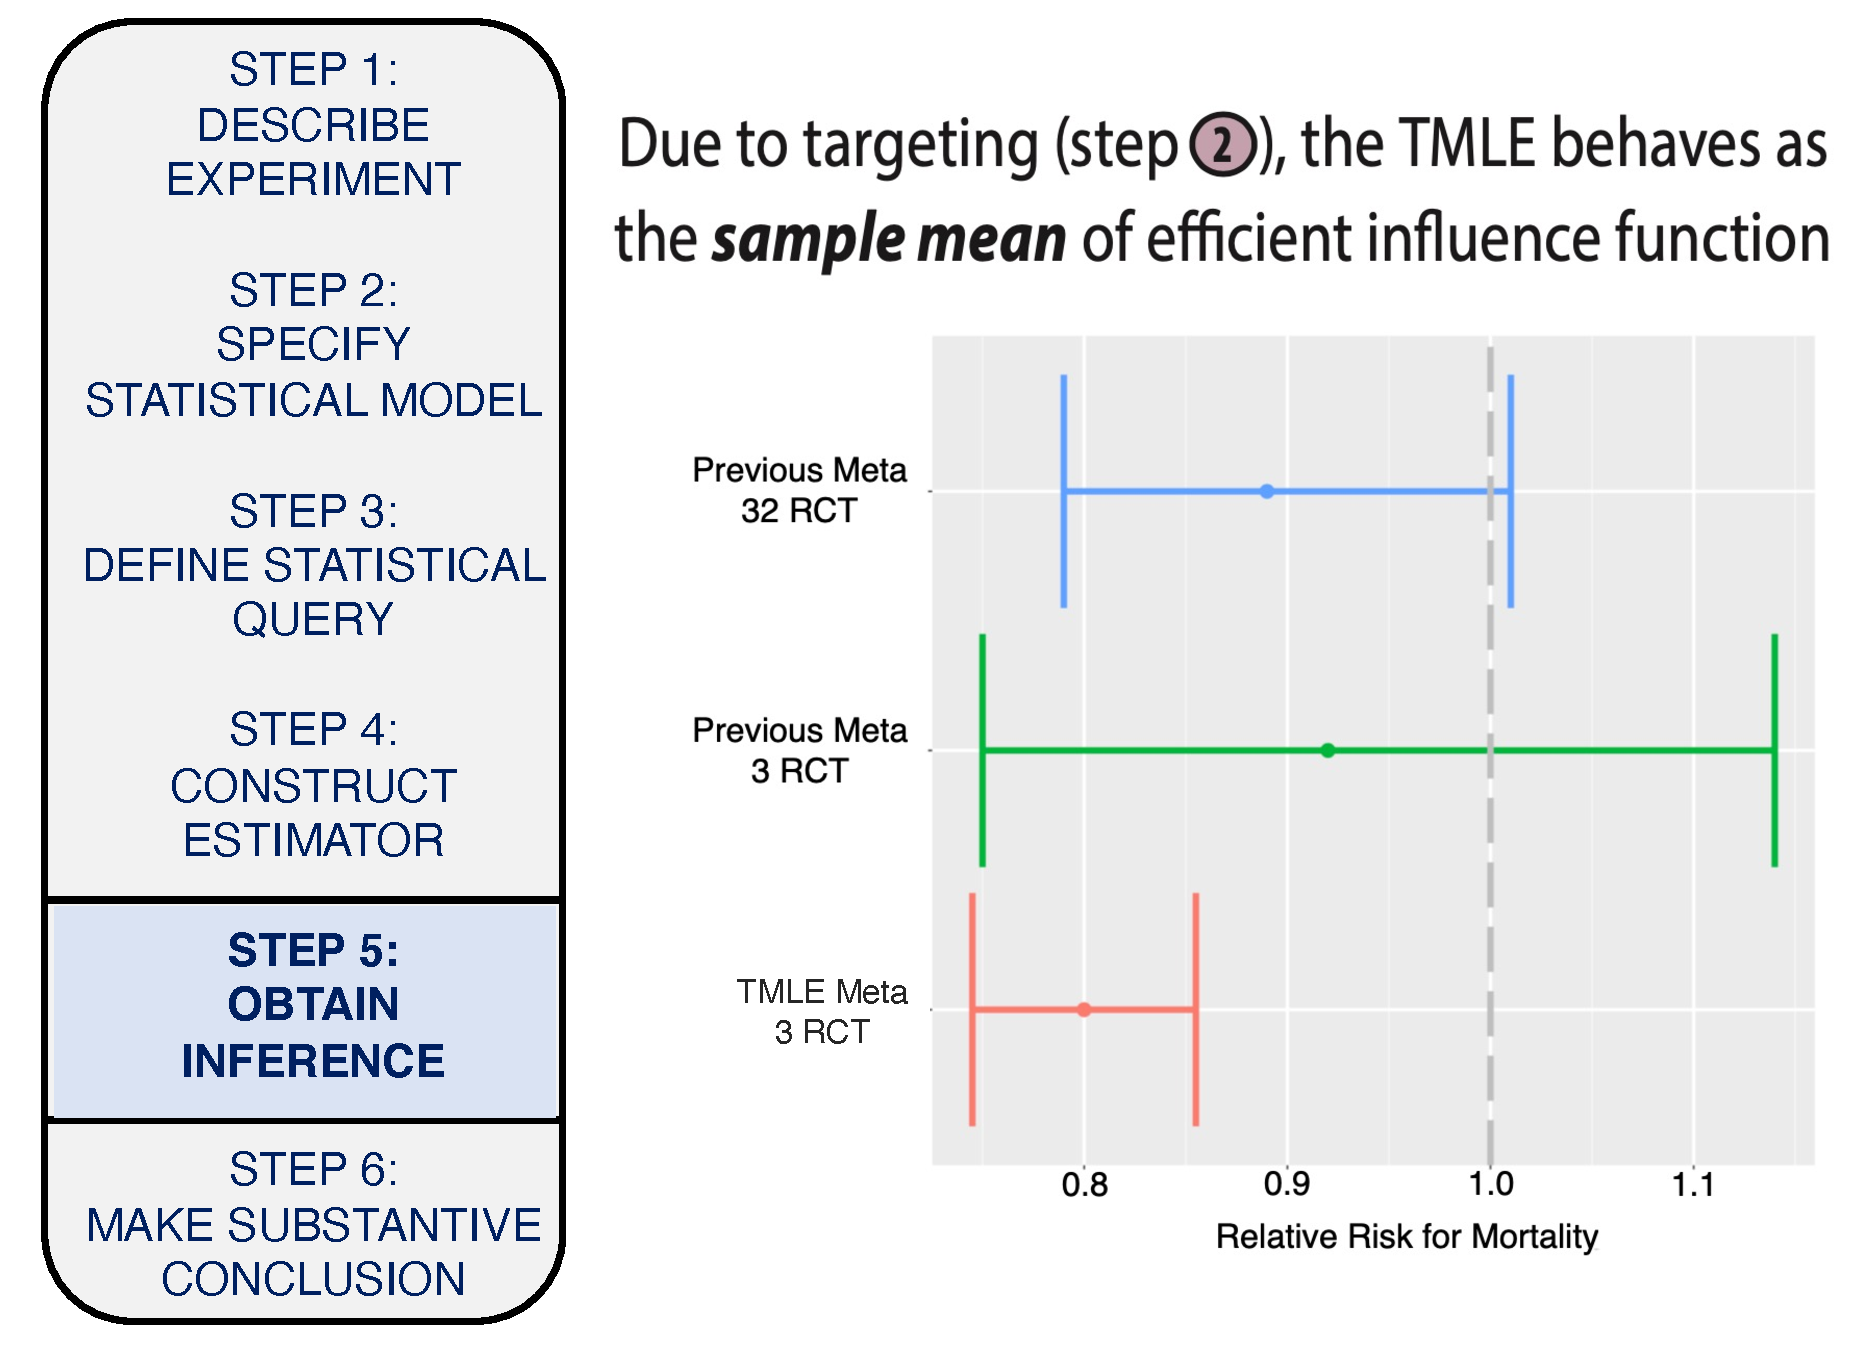
\includegraphics[width = 1.05\textwidth]{figures/roadmap5.pdf}
  \end{center}
\end{frame}

% \begin{frame}
%   \frametitle{TMLE Overview}
%   \begin{itemize}
%     \item TMLE produces an unbiased, efficient substitution estimator of target
%       parameters of a data-generating distribution $P_0$.
%     \item A TMLE algorithm is an iterative procedure that updates an initial
%       estimates of relevant components of $Q_0$ of $P_0$, often requiring an
%       estimate of a nuisance parameter $g_0$.
%       \begin{itemize}
%         \item Initial estimates of $(g_n, \bar{Q}_n)$ of nuisance parameters
%           $(g_0, \bar{Q}_0)$ may be obtained via super learning.
%         \item These initial estimates are then updated so that the relevant
%           component $\bar{Q}_n$ solves an estimating equation.
%       \end{itemize}
%     \item The updating step is a parametric fluctuation that updates $\bar{Q}_n$
%       to $\bar{Q}_n^{\star}$ based on the nuisance function $g_0$.
%   \end{itemize}
% \end{frame}

\begin{frame}
  \frametitle{Coding exercise: TMLE with \texttt{tmle3}}
  \url{https://tlverse.org/catalyst2024-workshop/tmle3.html}
\end{frame}

\subsection{Place conclusions in substantive context}

\begin{frame}
\frametitle{Arriving at the substantive conclusion}
\vspace{-16pt}
  \begin{center}
  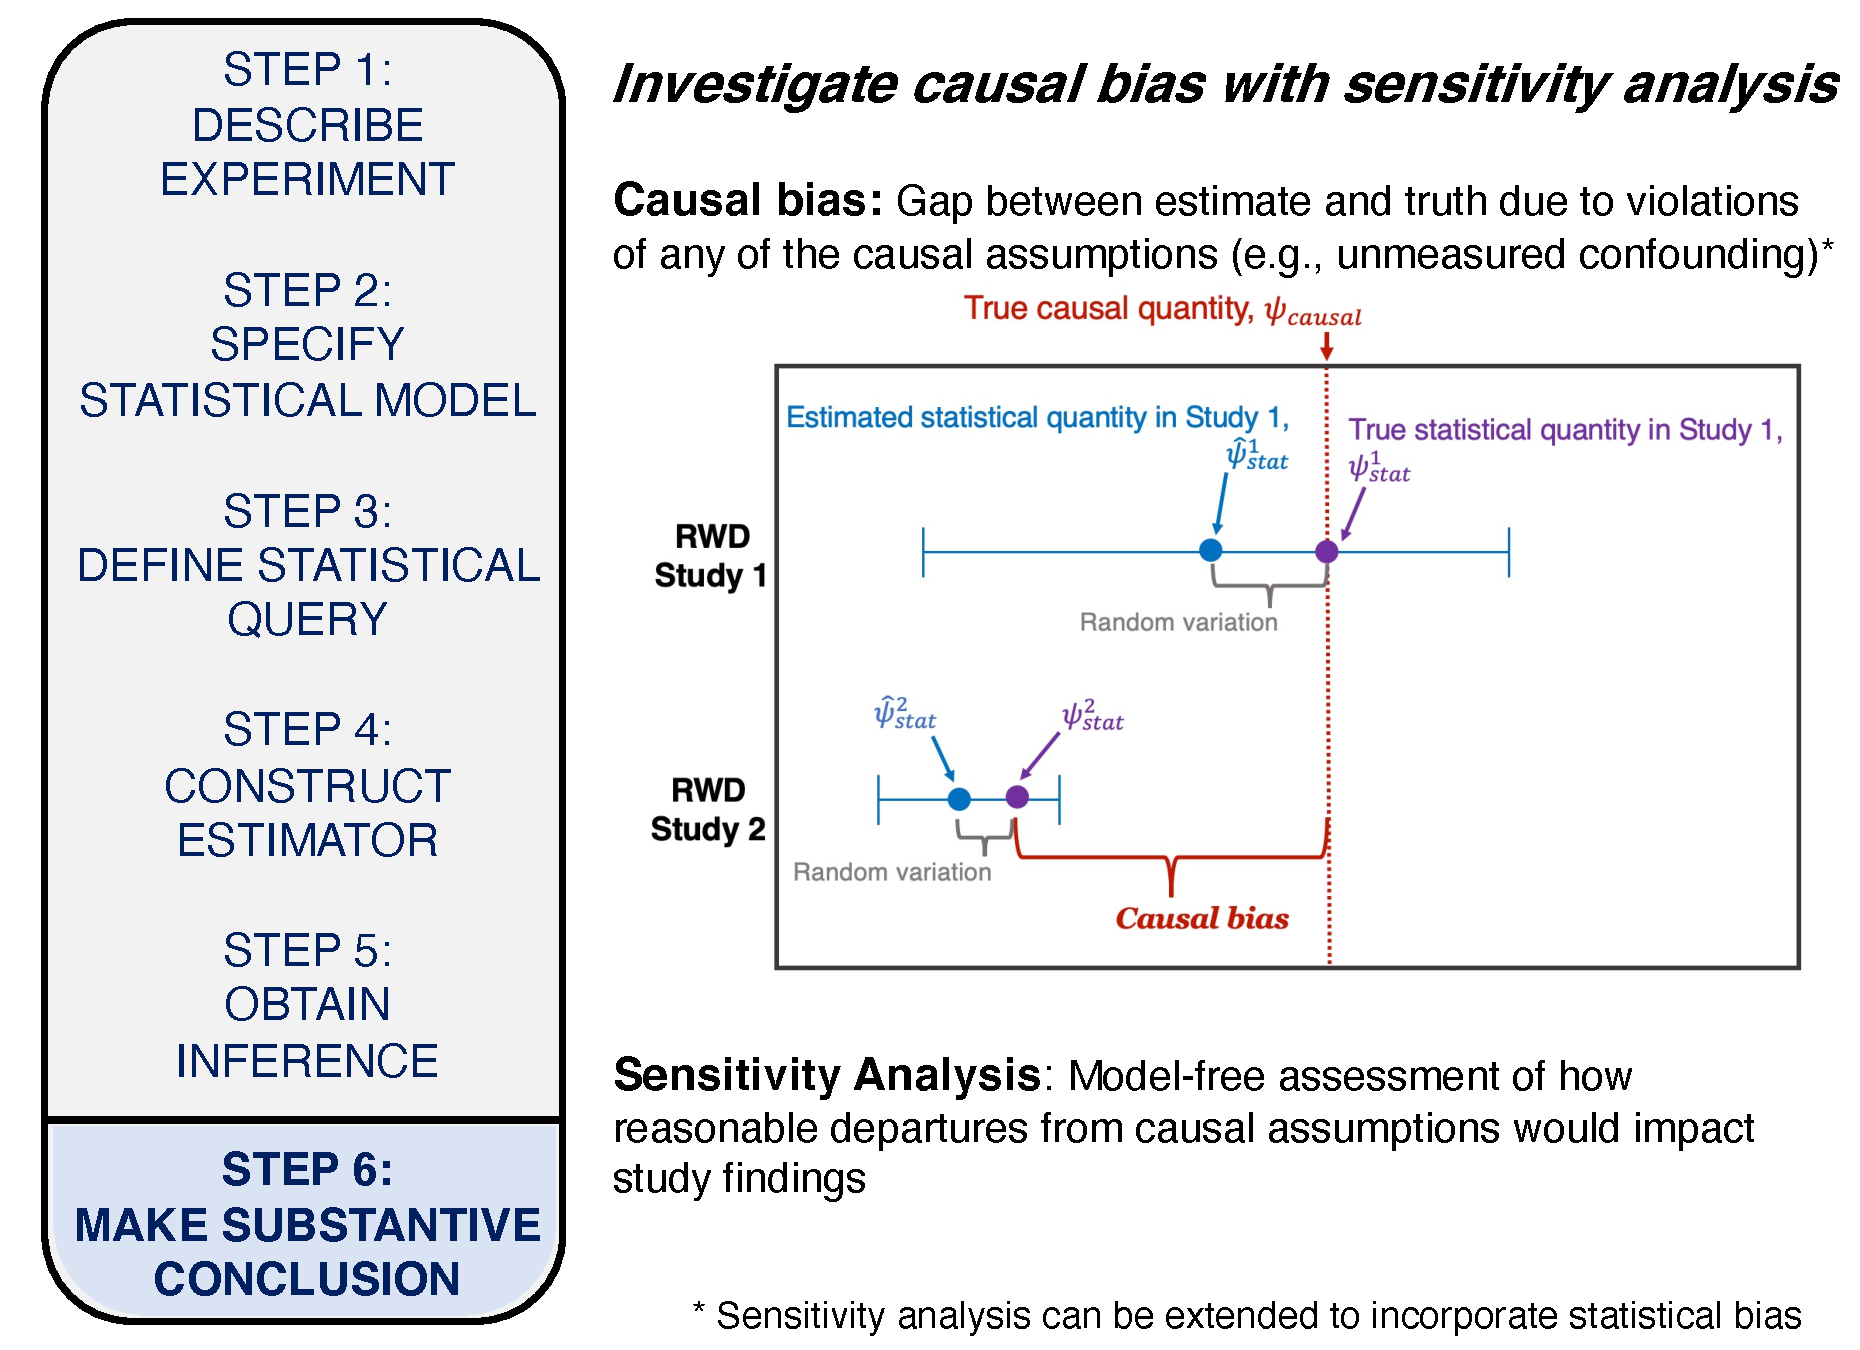
\includegraphics[width = 1.02\textwidth]{figures/roadmap6.pdf}
  \end{center}
\end{frame}

\begin{frame}
\frametitle{TL-based non-parametric sensitivity analysis: RCT with 25\% LTFU}
\vspace{-10pt}
  \begin{center}
  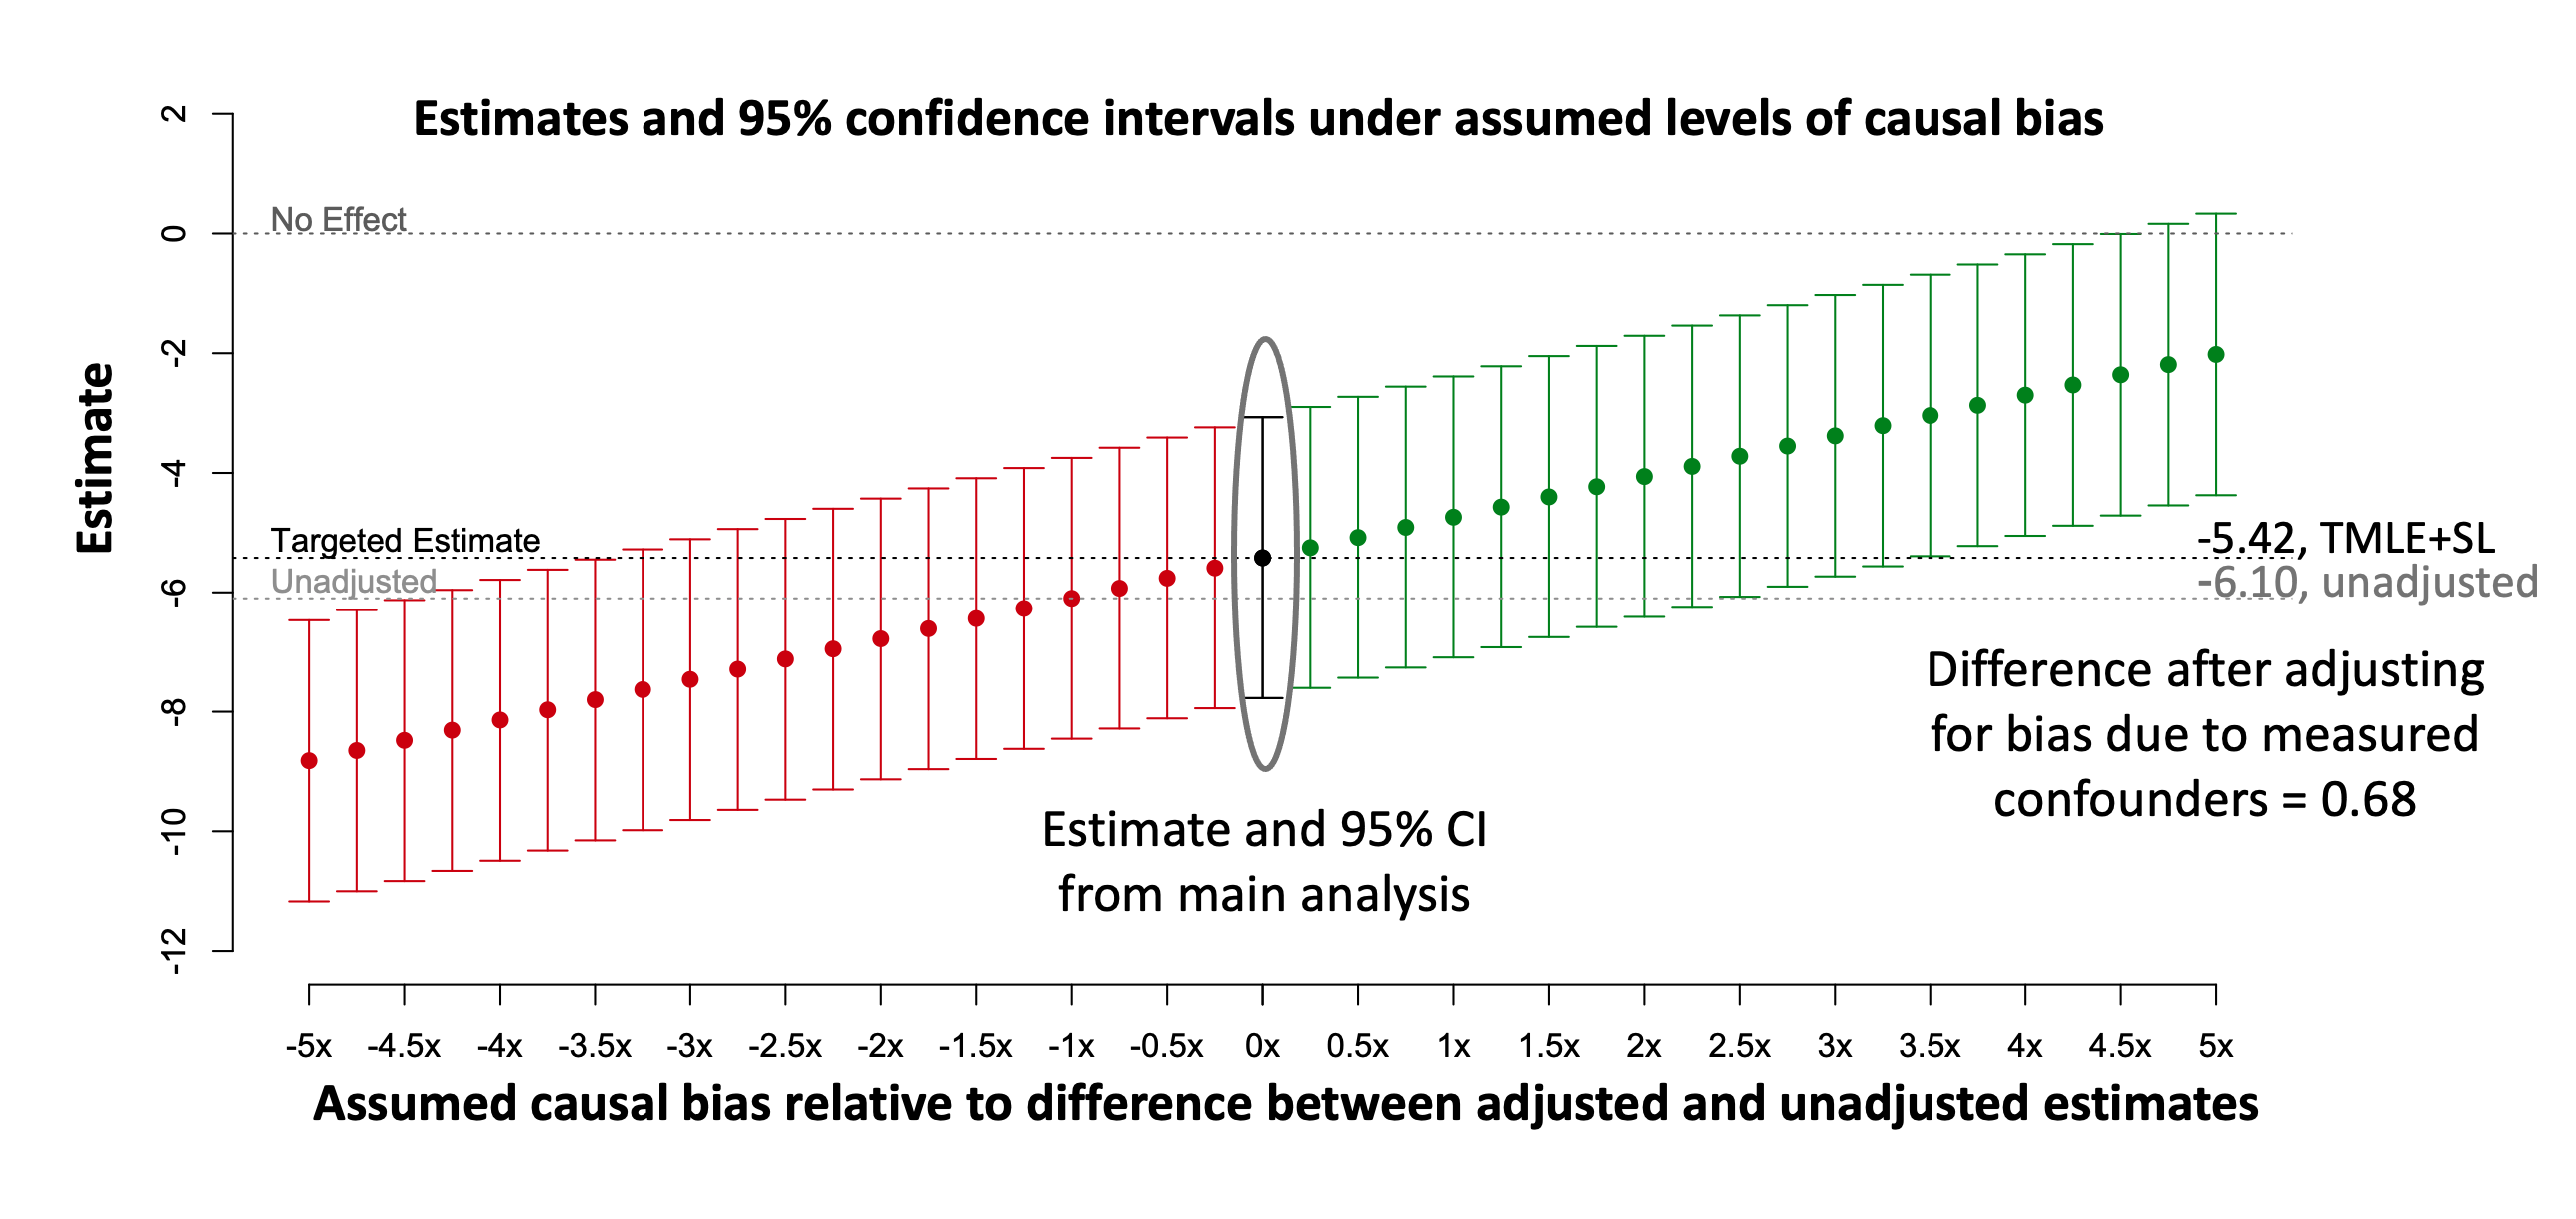
\includegraphics[width = 1.05\textwidth]{figures/gruber_sensitivity.png}
  \end{center}
  \vspace{35pt}
\tiny{Courtesy of ``Targeted-Learning Based Statistical Analysis Plan'' Webinar by Susan Gruber on 28 April 2021}
\end{frame}

\begin{frame}
\frametitle{TL-based non-parametric sensitivity analysis: Safety analysis example}

\vspace{-18pt}
  \begin{center}
  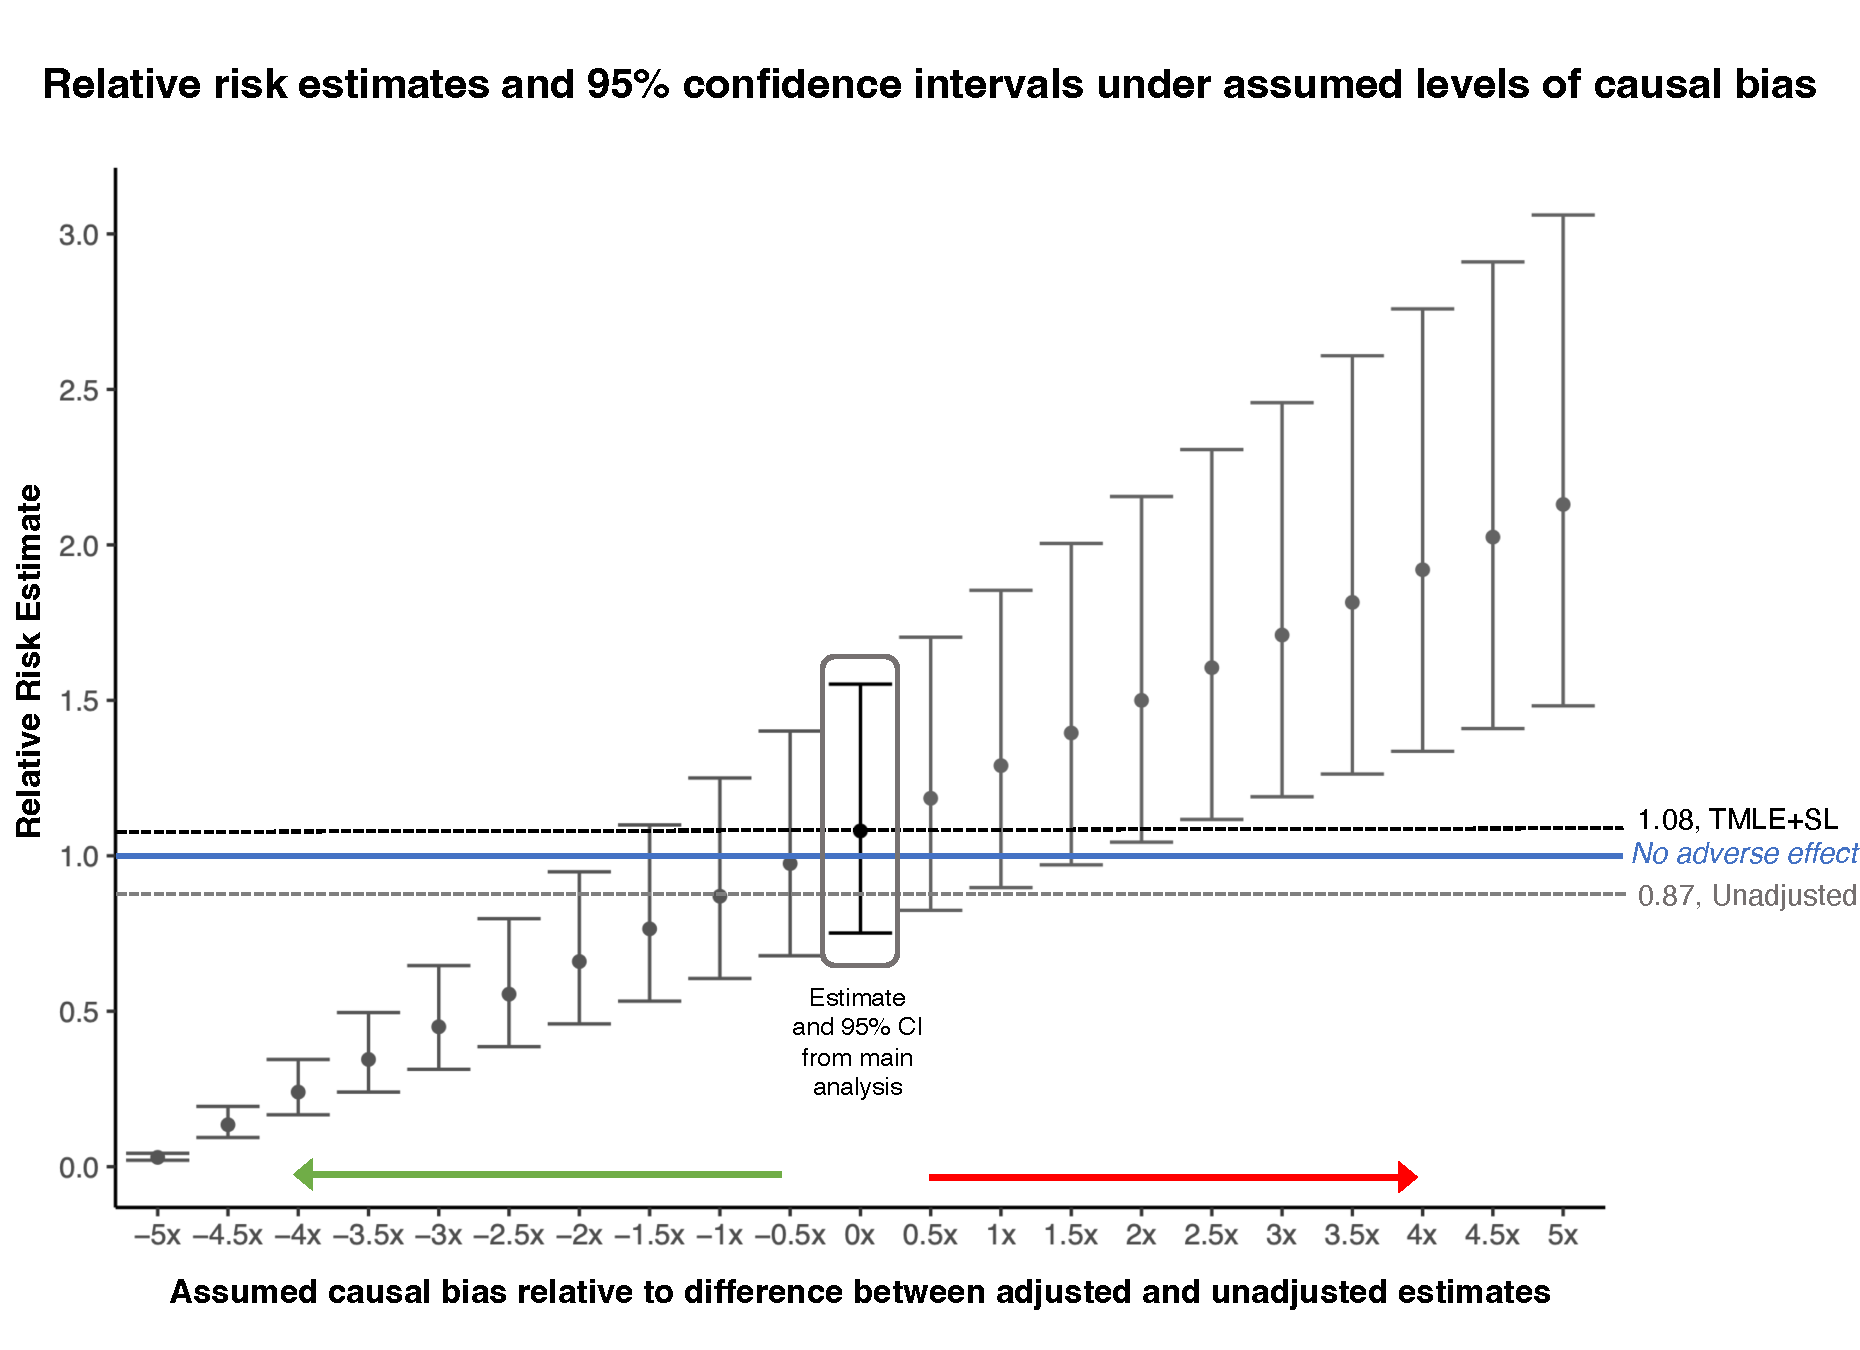
\includegraphics[width = 1.01\textwidth]{figures/sensitivityRR_greyscale.pdf}
  \end{center}
\end{frame}

\begin{frame}
  \frametitle{Possibility to refine question of interest and inform future studies}
  \vspace{-11pt}
  \begin{center}
  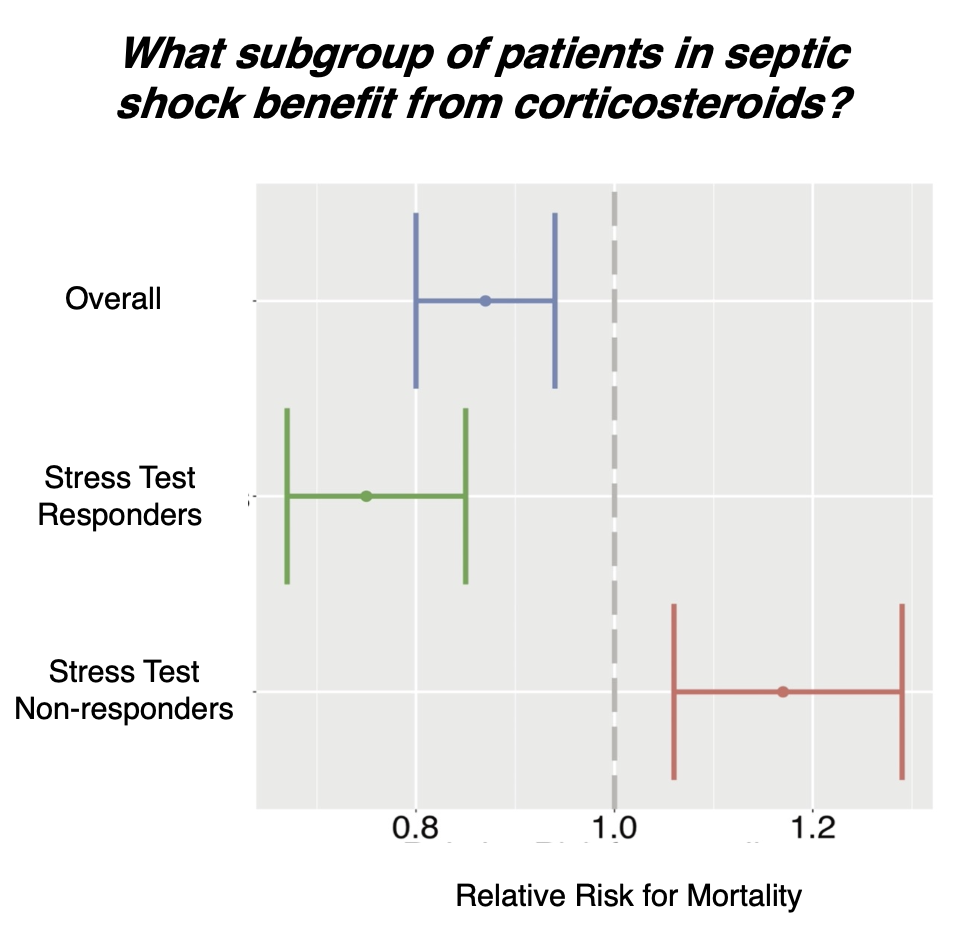
\includegraphics[width = 0.85\textwidth]{figures/subgroup.png}
  \end{center}
\end{frame}

\section{Advanced TL}

\subsection{Collaborative TMLE}

\begin{frame}
\frametitle{Outcome blind simulations to a priori define TMLE: Wyss et al., 2023}
\centering
\begin{figure}
\begin{center}
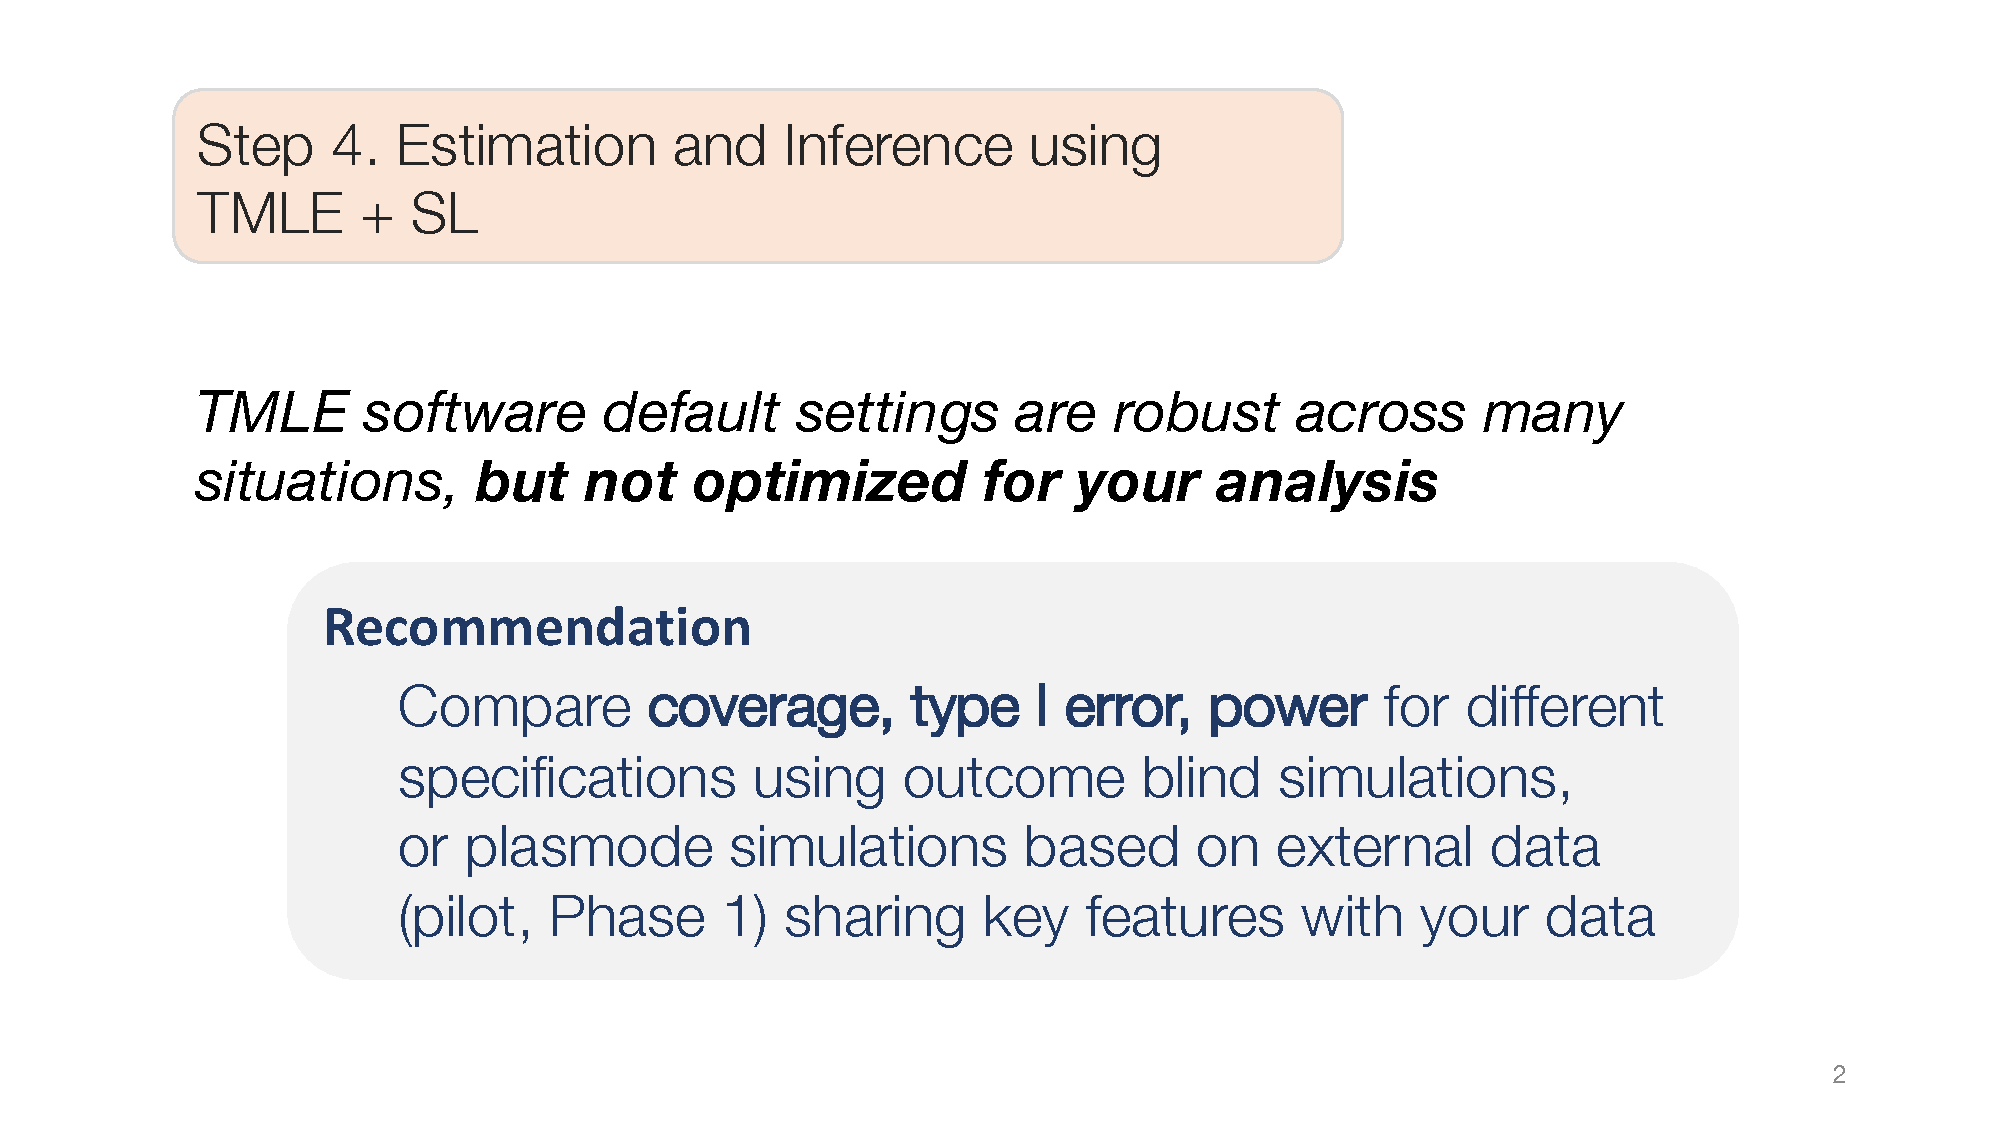
\includegraphics[width=1.02\textwidth]{figures/abbviepdfslides_2.pdf}
\end{center}
\end{figure}
%\vspace{35pt}
{\small R. Wyss et al. (2023). Targeted Learning with the Collaborative
Controlled Lasso for Large-Scale Covariate Adjustment in Healthcare Database
Studies}
\end{frame}

\begin{frame}
\centering
\begin{figure}
\begin{center}
\includegraphics[width=1.02\textwidth]{figures/abbviepdfslides_3.pdf}
\end{center}
\end{figure}
%\vspace{35pt}
\end{frame}

\begin{frame}{Outcome-regression weighted LASSO (OAL)}
Shortreed \& Ertefaie (2017) proposed outcome-regression weighted Lasso (OAL) for propensity score (PS) estimation:
\begin{itemize}
  \item  Fit unpenalized linear model for $\mathbb{E}(Y \mid A,W)$:
  $$(\hat{\alpha}, \hat{\eta}) = \arg\min_{\alpha,\eta} l_n(\alpha;Y,A,W).$$
where $\eta$ is the coefficient for $A$, and $\alpha$ is the coefficient for $W$.
\item Denote the coefficient for variable $W_j$ in the outcome regression with $\hat{\alpha}_j$.
\item Fit PS with Lasso using regularization term
\[
  \lambda \sum_j ||\alpha_j||^{-\gamma} ||\beta_j || \mbox{ instead of usual $\lambda \sum_j \mid \beta_j\mid$ \ . }
\]
%\item  They suggest $\gamma= 2 \cdot (3 - \lambda)$ to ensure the necessary conditions for the convergence properties.
\end{itemize}
\end{frame}

\begin{frame}
\frametitle{HAL-based OAL for PS Estimation}
The theoretical property of OAL relies on the \textbf{\textit{correct parametric formula}}, which is often unknown in practice.
We extend OAL to outcome-regression weighted HAL (OHAL):
\begin{enumerate}
\item Compute the outcome regression using Lasso of form $\sum_j \alpha_n(j)\phi_j(W,A)$.
%with dependent variable the outcome $Y$ and features the basis functions $\phi_j(A,W)$ and the treatment indicator $A$.
\item Use as basis functions for the PS $\{\phi_j(1,W),\phi_j(0,W): j\}$.
\item Both of these two basis functions will be associated with same weight $\alpha_n(j)$.
%The $L_1$ constraint parameter $M^{(1)}$ can be selected by CV.
\item Compute the propensity score using a Lasso logistic regression using the above basis functions.  The $L_1$-constraint for $\beta_{j}$'s, the coefficient for $\phi_j$, is defined as the weighted $L_1$-norm above.
\item Or simply define $\lVert \beta \rVert_1=\sum_{j, \alpha_n(j)\not =0}\mid \beta(j)\mid$.
%  $$\sum_{s \subset \{1, %\cdots,n\}}\sum_{i=1}^{n}|\alpha_{s,i}|^{-\gamma} |\beta_{s,i}| < %M^{(2)}$$
\end{enumerate}
\end{frame}
\begin{frame}{C-TMLE to select $L_1$-norm}
\begin{itemize}
  \item Tune the $L_1$-norm with C-TMLE: i.e. optimize in $\lambda$ increase in likelihood of TMLE-step using $g_{n,\lambda}$.
  \item Can be combined with standard lasso to yield a collaborative-controlled (CC) regularization for TMLE.
  \item Similarly can be used in a collaborative-controlled outcome-adaptive lasso (CC-OAL) for TMLE.
\end{itemize}
\end{frame}

\begin{frame}
\centering
\begin{figure}
\begin{center}
\includegraphics[width=1.02\textwidth]{figures/abbviepdfslides_6.pdf}
\end{center}
\end{figure}
%\vspace{35pt}
\end{frame}

\begin{frame}
\centering
\begin{figure}
\begin{center}
\includegraphics[width=1.02\textwidth]{figures/abbviepdfslides_7.pdf}
\end{center}
\end{figure}
%\vspace{35pt}
\end{frame}

\begin{frame}
\centering
\begin{figure}
\begin{center}
\includegraphics[width=1.02\textwidth]{figures/abbviepdfslides_8.pdf}
\end{center}
\end{figure}
%\vspace{35pt}
\end{frame}

\subsection{HAL and A-TMLE}

\begin{frame}
\frametitle{Zero-order Highly Adaptive Lasso (HAL): A nonparametric MLE}
\begin{block}{\large{Key Idea}}
\begin{itemize}
\vspace{.1in}
\item Any $d$-dimensional cadlag function (i.e.~right-continuous, left limits)
can be represented as an infinite linear combination of spline basis functions.
\vspace{.05in}
\item The variation norm / complexity of a function is the $L_1$-norm of the vector of coefficients.
\vspace{.1in}
\end{itemize}
\end{block}
\vspace{0.25in}
\begin{center}
{\large Zero-order HAL converges to true function at rate $n^{-1/3}(\log n)^{d/2}$ (only assuming finite variation norm)}
\end{center}
\end{frame}

\begin{frame}{Formal representation of cadlag function as linear combination of zero-order splines}
\begin{itemize}
\item A cadlag function $f\in D^{(0)}([0,1]^d)$ can be represented as
\[
f(x)=f(0)+\sum_{s\subset\{1,\ldots,d\}}\int_{(0_s,x_s]}df_s(u),\]
where $f_s(x_s)=f(x(j)I(j\in s): j=1,\ldots,d)$ is the section implied by setting coordinates outside $s$ equal to zero, and $x_s=(x(j): j\in s)$.
\item Moreover, we define the sectional variation norm of $f$ as the sum over $s$ of the variation norms of $f_s$:
\[
\lVert f\rVert_v^{\star}=\sum_s \lVert f_s \rVert_v=\mid f(0)\mid +\sum_s
\int_{(0_s,1_s]}\lvert df_s(u)\rvert \ .
\]
\end{itemize}
\end{frame}
\begin{frame}
\begin{itemize}
\item Now, notice that this writes $f$ as an infinite linear combination of $x\rightarrow I(x_s\geq u)$ of zero order splines with knot-point $u\in (0_s,1_s]$ and coefficient $df_s(u)$, and that the sectional variation norm is the $L_1$-norm in this representation.
\end{itemize}
\end{frame}

\begin{frame}
\frametitle{Zero-order HAL performance for d=3}
  \vspace{-10pt}
  \begin{center}
  \includegraphics[width = 1\textwidth]{figures/HALworks.png}
  \end{center}
\end{frame}

\begin{frame}{HAL Provides Estimators of Large Variety of Nuisance Parameters Needed in Causal Inference}
\begin{itemize}
\item Causal Inference requires statistical estimation of nuisance functions.
\item In particular, it requires  estimation of conditional means; conditional  densities or cumulative distribution functions; intensities, conditional hazards. Standard loss functions can be employed for these.
\item Moreover, it is often possible to define risk functions that define  target functions of interest itself. For example, a variety of risk functions have been proposed for the conditional treatment effect. One can then apply HAL to minimize the empirical risk function.
\item In these cases,  estimation of the empirical risk function requires itself nuisance parameter estimation, where again HAL could be used.
\end{itemize}
\end{frame}

\begin{frame}{How to develop a HAL-MLE: parametrize target function in terms of unrestricted function}
\begin{itemize}
\item Suppose one is interested in a functional parameter $Q(P)$  such as a conditional density.
\item Select a loss function or risk function so that $Q(P)=\arg\min_Q R_P(Q)$, where, for example, $R_P(Q)=PL(Q)$ for some loss $L(Q)$.
\item $Q$ might be constrained in some ways. Therefore, find a parametrization $Q=Q_f$ in terms of an unconstrained function $f$. For example, parametrize a conditional density in terms of conditional hazard and represent the latter as $\exp(f)$.
\item Now, model $f$ as a linear combination of zero order splines and compute the MLE
$\beta_n=\arg\min_{\beta,\lVert\beta\rVert_1<C_n}R_n\left (Q_{\sum_j \beta(j)\phi_j}\right)$,
where $R_n(Q)$ is an estimate of the risk $R_{P_0}(Q)$ such as $R_n(Q)=P_n L(Q)$.
\item The HAL-MLE of $Q_0$ is then given by $Q_n=Q_{f_n}$ with $f_n=\sum_j\beta_n(j)\phi_j$.
\end{itemize}
\end{frame}

\begin{frame}{Additive models within the cadlag function space to define subspace specific HALs}
\begin{itemize}
\item Instead of selecting the richest set of basis function such as the ones implied by knot-points
$\{X_i(s): i=1,\ldots,n,s\subset\{1,\ldots,d\}\}$, one can only model a subset ${\cal S}_1$ of all the additive functions $\tilde{f}_s(x_s)=\int I(x_s\geq u) df_s(u)$  by not including all subsets $s$ in ${\cal S}_1$.
\item If ${\cal S}_1$ represents the collection of all subsets we include, then this defines additive models $f(x_s)=f(0)+\sum_{s\in {\cal S}_1}\tilde{f}_s(x_s)$. One can then define a corresponding HAL-MLE $f_{n,{\cal S}_1}$.
\item More generally, we define $D^{(0)}({\cal R}^{0,*})$ as the linear span of $\{\phi_j: j\in {\cal R}^{0,*}\}$, and by choosing the richest set ${\cal R}^0$, we have $D^{(0)}({\cal R}^0)=D^{(0)}([0,1]^d)$.
\item We use $D^{(0)}_M({\cal R}^{0,*})$ when bounding $L_1$-norm by $M$.
\end{itemize}
\end{frame}
\begin{frame}
\begin{itemize}
\item Every choice of subset of basis functions then implies an HAL-MLE.
\item One could also first use an initial ML-algorithm, such as MARS, to learn the family of subsets, ${\cal S}_1$, that appears to be needed, and then compute the resulting HAL-MLE $f_{n,{\cal S}_1}$.
\item Of course, the screening algorithm is then part of algorithm, which needs to be respected when using cross-validation to select the $L_1$-norm or select tuning parameter of the initial screening.
\end{itemize}
\end{frame}

\begin{frame}{Rate of convergence of zero order HAL}
\begin{itemize}
\item Let $Q_n=Q_{f_n}$ be the HAL-MLE.
\item Let $d_0(Q,Q_0)=P_0L(Q)-P_0L(Q_0)$ be the loss based dissimilarity.
\item We  have
\begin{eqnarray*}
d_0(Q_n,Q_0)&=&P_n\{ L(Q_n)-L(Q_0)\}\\
&&-(P_n-P_0)\{L(Q_n)-L(Q_0)\}\\
&\leq &- (P_n-P_0)\{L(Q_n)-L(Q_0)\}.
\end{eqnarray*}
\item Let ${\cal F}=\{L(Q_f)-L(Q_0):f\in D^{(0)}_M([0,1]^d)\}$.
\item The (known) covering number for $D^{(0)}_M([0,1]^d)$ implies the same covering number for ${\cal F}$.
\end{itemize}
\end{frame}

\begin{frame}{Using empirical process theory:}
\begin{itemize}
\item Let ${\cal F}(\delta)=\{f\in {\cal F}: P_0f^2\leq \delta^2\}$.
\item $\sup_{f\in {\cal F}(\delta)}\mid n^{1/2}(P_n-P_0)f\mid$ can be bounded by  the entropy integral
$J(\delta,{\cal F}(\delta))=\int_{(0,\delta]}\sqrt{\log N(\epsilon,{\cal F},L^2)} d\epsilon$, which behaves as $\delta^{1/2}$ up till $\log \delta$-factor.
\item Using that $P_0(L(Q)-L(Q_0)))^2\leq C d_0(Q,Q_0)$, we can then apply an iterative proof bounding
\begin{eqnarray}
d_0(Q_n,Q_0)&\leq& n^{-1/2}\sup_{f\in {\cal F}(\delta^k)}\mid n^{1/2}(P_n-P_0)f\mid\\
&\sim & n^{-1/2} J(\delta^k,{\cal F}),
\end{eqnarray}
 starting with $\delta^0=1$, $\delta^1=n^{-1/4}$, and so on.
  \end{itemize}
 \end{frame}
 \begin{frame}
 \begin{itemize}
 \item The monotone improving (in rate) sequence converges to the fixed point $\delta^*$ of equation
 \[
 \delta^2=n^{-1/2}J(\delta,{\cal F}).\]
 \item
This $\delta^{\star}$ equals the rate of convergence for $d_0^{1/2}(Q_n,Q_0)$.
\item We find $d_0(Q_n,Q_0)=O_P(n^{-2/3}(\log n)^d)$.
\end{itemize}
\end{frame}

\begin{frame}
\frametitle{Basic \texttt{R} \texttt{hal9001} Functionality}
\begin{enumerate}
    \item Load package and data: \newline \texttt{library(hal9001)} \newline
    \texttt{data(mtcars)}
    \item Create numeric vector for dependent variable: \newline \texttt{Y <-  mtcars[,"mpg"]}
    \item Create dataframe or matrix of predictors: \newline
    \texttt{X <- mtcars[,c("cyl", "disp", "hp", "wt")]}
    \item Fit HAL: \newline
   \texttt{ hal\_fit <- fit\_hal(X=X, Y=Y)}\newline
   \newline
   \small{\textit{Note}: default \texttt{max\_degree=3} considers no more than 3-way interactions, and default \texttt{reduce\_basis=0} places no restrictions on the minimum proportion of 1's in basis functions.}
\end{enumerate}
\end{frame}

\begin{frame}
\frametitle{Summary table of \texttt{hal9001}  HAL fit}
\vspace{-2pt}
\texttt{summary(hal\_fit)\$table}
\begin{center}
\vspace{-2pt}
\includegraphics[width = 0.38\textwidth]{figures/HAL-summary-mtcars.png}
\end{center}
\end{frame}

\begin{frame}
\frametitle{Specifying \texttt{hal9001} model formulas}
\textit{Example}: Observe $O=(W_1, W_2, A, Y) \sim P_0$ \newline
$$\text{\texttt{R} code: \texttt{fit\_hal(Y, X, formula, data, ...)}} $$
\textbf{Additive model \texttt{formula}}: \newline
$\text{\texttt{Y}} \sim . $ or $\text{\texttt{Y}} \sim \text{\texttt{h(W1) + h(W2) + h(A)}} $
\vspace{0.05in}
\textbf{Bi-additive model \texttt{formula}}: \newline
$\text{\texttt{Y}} \sim . $\^{}$\text{\texttt{2}}$ or $\text{\texttt{Y}} \sim \text{\texttt{h(W1)+h(W2)+h(A)+h(W1,W2)+h(W1,A)+h(W2,A)}}$
\vspace{0.05in}
\textbf{Only interactions with A \texttt{formula}:} \newline
$\text{\texttt{Y}} \sim \text{\texttt{h}}(.) + \text{\texttt{h}}(.\text{\texttt{,A}})$ or $\text{\texttt{Y}} \sim \text{\texttt{h(W1)+h(W2)+h(A)+h(W1,A)+h(W2,A)}}$
\vspace{0.05in}
\textbf{Monotone $\uparrow$ (i) $\downarrow$ (d) \texttt{formula} examples}:
$\text{\texttt{Y}} \sim \text{\texttt{i}}(.) $ or $\text{\texttt{Y}} \sim \text{\texttt{i}}(.) + \text{\texttt{i}}(.,.) $ or
$\text{\texttt{Y}} \sim \text{\texttt{i(W1)+d(W2)+i(A)}}$
%\newline
%\newline
\end{frame}

\begin{frame}
\frametitle{Possible HAL fits under various smoothness orders}
\textit{Example}: Observe $(W, A, Y) \sim P_0$
$$\text{\texttt{R} code: \texttt{fit\_hal(Y, X, data, formula, k, ...)}} $$
\textbf{Example fits for 0-order smoothness, \texttt{k=0}}: \newline
    Additive model:

    $Y = \mathbb{I}(W>0.5) + \mathbb{I}(W > 0.3) + \mathbb{I}(A>0)$ \newline
    Bi-additive model:

    $Y = \mathbb{I}(W>0.5) + \mathbb{I}(A>0)  + \mathbb{I}(W>0.5, A>0)$
    \newline
    \newline
\textbf{Example fits for 1st-order smoothness, \texttt{k=1}}: \newline
Additive model:

$Y = \mathbb{I}(W>0.5)[W - 0.5] + \mathbb{I}(W>0.3)[W - 0.3] + \mathbb{I}(A>0)[A-0]$
  \newline
 Bi-additive model:

 $Y = \mathbb{I}(W>0.5)[W - 0.5] + \mathbb{I}(A>0)[A-0]  + \mathbb{I}(W>0.5, A>0)[W - 0.5][A - 0]$ \newline
\end{frame}

\begin{frame}{Derivation of first-order spline representation of cadlag function}
\begin{itemize}
\item In the presentation of $f\in D^{(0)}_M([0,1]^d)$ there appear integrals
$\int_{(0(s),x(s)]} df_s(u)$.
\item Assume and write $df_s(u)=df_s/du du$; assume the RN-derivative $f_s^{(1)}=df_s/du\in D^{(0)}_M([0,1]^d)$, and plug-in the zero order spline representation for
\[
  f_s^{(1)}(u)=f_s^{(1)}(0)+\sum_{s_1\subset s}\int_{(0(s_1),u(s_1)]}
  df_{s_1}^{(1)}(u_1).
\]
\item Apply Fubini's theorem to the double integrals over $(u,u_1)$ to obtain
a representation in terms of tensor products of {\bf first} order splines.
\end{itemize}
\end{frame}

\begin{frame}
\begin{itemize}
\item As an example, let's do it for a univariate function:
\[
\begin{array}{l}
f(x)=f(0)+\int_{(0,x]} df(u)\\
= f(0)+\int_{(0,x]} f^{(1)}(u) du\\
=f(0)+\int_{(0,x]} \{f^{(1)}(0)+\int_{(0,u]} df^{(1)}(u_1)\} du\\
= f(0)+x f^{(1)}(0)+\int_{u_1}\int_u I(u\leq x) I(u_1\leq u) du df^{(1)}(u_1)\\
=f(0)+f^{(1)}(0) x+\int_{u_1} I(x\geq u_1)(x-u_1) df^{(1)}(u_1),
\end{array}
\]
which is a linear combination of first order splines $\phi^1_{u_1}(x)=I(x\geq u_1)(x-u_1)$, including $\phi^1_0(x)=x$ implied by knot-point $u_1=0$.
\end{itemize}
\end{frame}

\begin{frame}
\begin{itemize}
\item In this manner we obtain the following first order spline representation for a function
$f\in D^{(1)}([0,1]^d)$ (a cadlag function satisfying our first orders smoothness assumption):
\[
\begin{array}{l}
f(x)=f(0)+\sum_{s\subset \{1,\ldots,d\}} \phi^1_0(x(s))f^{(1)}_s(0)\\
+
\sum_{s,s_1\subset s, \mid s_1\mid>0}\bar{\phi}_{s,s_1}(x)\int \phi^1_{u(s_1)}(x(s_1)) f^{(1)}_{s,s_1}(du).\end{array}
\]
\item Here $\bar{\phi}_{s,s_1}(x(s/s_1))=\prod_{l\in s/s_1}x(l)$ and $f^{(1)}_{s,s_1}$ is the $s_1$-section of $f^{(1)}_s=df_s/du$.
\end{itemize}
\end{frame}

\begin{frame}
\begin{itemize}
\item Notice that finite linear part in this representation of $f$ is just parametric model in $x_1,\ldots,x_d$ and its interactions (e.g., for $d=2$, $x_1,x_2,x_1x_2$. The remaining infinite linear part is linear combination in tensor products of first order splines with interior knot-points in $(0(s_1),1(s_1)]$ while having knots at 0 for components $x_j$ with $j\in s/s_1$.
\item The $L_1$-norm  of all coefficients $f^{(1)}_{s,s_1}(du)$ and
$f^{(1)}_s(0)$ defines our first order sectional variation norm $\lVert f\rVert_{v,1}^{\star}$.
\item $D^{(1)}_M([0,1]^d)$ is defined as all functions $f\in D^{(0)}([0,1]^d)$
satisfying this first order smoothness with $\lVert f\rVert_{v,1}^{\star}\leq M$.
\end{itemize}
\end{frame}

\begin{frame}{(fine enough) Finite dimensional first order spline working model}
\begin{itemize}
\item For each $s\subset\{1,\ldots,d\}$, we can select knot-points
${\cal R}^1(s)\equiv  \{(0(s/s_1),X_i(s_1)): i=1,\ldots,n,s_1\subset s\}\subset [0(s),1(s)]$. The corresponding first order splines are:
\[
\{\phi^1_{u(s)}: u(s)\in {\cal R}^1(s)\}.\]
For $s_1$ the empty set this yields  $\{0(s): s\subset\{1,\ldots,d\}\}$, giving the interactions $\phi^1_{0(s)}=\prod_{j\in s}x_j$.
\item The total set of $N$ first order splines is thus;
\[
{\cal R}^1_N\equiv \{\phi^1_{u(s)}: u(s)\in {\cal R}^1(s), s\subset \{1,\ldots,d\}\}.\]
\end{itemize}
\end{frame}

\begin{frame}
\begin{itemize}
\item The initial starting model of linear combinations of first order splines is then:
\[
D^{(1)}({\cal R}^1_N)=\left\{\sum_{j\in {\cal R}^1_N}\beta(j)\phi_j: \beta\right\}.\]
\item This working model $D^{(1)}({\cal R}^1_N)\subset D^{(1)}([0,1]^d)$ represents a close approximation of $D^{(1)}([0,1]^d)$ (providing sup-norm approximations going as fast as $n^{-1/2}$).
\end{itemize}
\end{frame}

\begin{frame}{First-order spline HAL}
\begin{itemize}
\item We then define
\[
\beta_n=\arg\min_{\beta,\mid \beta\mid_1\leq C_n} P_n L(Q_{f_{N,\beta}}),\]
and first order HAL $Q_n=Q_{f_{N,\beta_n}}$.
\end{itemize}
\end{frame}

\begin{frame}{Rate of convergence for first order HAL}
\begin{itemize}
\item One can select $J$ zero order splines ${\cal R}^0(J)$ so that  $D^{(0)}({\cal R}^0(J))$ yields a $O^+(1/J)$ $L^2$-approximation of
$D^{(0)}([0,1]^d)$.
\item This explains the dimension free rate of convergence $O^+(n^{-1/3})$ for the zero-order HAL.
\item One can select $J$ first order splines, ${\cal R}^1(J)$, so that $D^{(1)}({\cal R}^1(J))$ yields a $O^+(1/J^2)$ {\bf supremum norm} approximation of $D^{(1)}([0,1]^d)$.
\item The entropy integral $J(\delta, D^{(1)}_M([0,1]^d),\lVert \cdot \rVert_{\infty})=O^+( \delta^{3/4})$ instead of $O^+(\delta^{1/2})$ for $D^{(0)}_M([0,1]^d)$.
\item Our rate of convergence proof  yields
\[
  d_0(Q_n,Q_0)=O_P^+(n^{-4/5}) \ .
\]
\end{itemize}
\end{frame}

\begin{frame}{New Results on higher order HAL-MLE}
\begin{itemize}
\item So first order HAL converges at rate $n^{-2/5}$ pointwise, ignoring $\log n$-factors.
\item At cost of another $\log n$-factor this rate is uniform in $x$.
\item Pointwise and simultaneous  confidence intervals follow.
\item Any of these HAL-estimators result in plug-in estimators of smooth target features that converge at $n^{-1/2}$ and are asymptotically normal, and either efficient and super-efficient (on set of measure zero!).
\item Inference can be based on nonparametric bootstrap.
\end{itemize}
\end{frame}

\begin{frame}{Efficient HAL-TMLE (vdL, Rubin, 2006)}
\begin{itemize}
\item Construct initial estimator ${\bf P}_n$; determine a least favorable path $\{{\bf P}_{n,\epsilon}:\epsilon\in (-\delta,\delta)\}\subset {\cal M}$ through ${\bf P}_n$ with score $D^*_{{\bf P}_n}$ at $\epsilon =0$.
\item Compute MLE $\epsilon_n =\arg\max_{\epsilon}P_n L({\bf P}_{n,\epsilon})$, where $L(P)$ is a valid loss function so that $\Psi(\arg\min_P P_0L(P))=\Psi(P_0)$.
\item Let ${\bf P}_n^*={\bf P}_{n,\epsilon_n}$. The TMLE is given by $\Psi({\bf P}_n^*)$.
\item By construction, $\Psi({\bf P}_n^*)-\Psi(P_0)=(P_n-P_0)D^*_{{\bf P}_n^*}+R({\bf P}_n^*,P_0)$, with $R(P,P_0)\equiv \Psi(P)-\Psi(P_0)-(P-P_0)D^*_P$ an exact second order remainder.
\item Using the Highly Adaptive Lasso as initial estimator ${\bf P}_n$, we are guaranteed that $\Psi({\bf P}_n^*)$ is asymptotically efficient estimator of $\Psi(P_0)$ (van der Laan, 2017).
\end{itemize}
\end{frame}

\begin{frame}{HAL-TMLE of Target Estimands is Asymptotically Efficient}
\begin{itemize}
\item TMLE is two-stage method for constructing plug-in efficient estimators $\Psi(P_n^*)$ of  a pathwise differentiable target estimand $\Psi(P_0)$.
\item
The HAL-TMLE (using HAL as initial estimator) is efficient in great generality (vdL, 15).
\item  The only necessary model assumptions are:
\begin{itemize}
\item The true nuisance parameters have finite sectional variation norm
\item The loss functions of the true nuisance parameters are uniformly bounded, so that oracle inequality applies
\item The strong positivity assumption holds
\end{itemize}
\end{itemize}
\end{frame}

\begin{frame}{Example: Asymptotic  efficiency of (zero-order) HAL-TMLE for treatment-specific mean / ATE}
Consider the HAL-TMLE of $EY_1=EE(Y\mid A=1,W)$ based on $(W,A,Y)\sim P_0$ in a nonparametric statistical model.
\vspace{0.15in}
It is asymptotically efficient if
\begin{enumerate}
\item $\delta<P_0(A=1\mid W)$ for some $\delta>0$
\item $W\rightarrow E_0(Y\mid A=1,W)$  and $W\rightarrow P_0(A=1\mid W)$ are cadlag
\item $W\rightarrow E_0(Y\mid A=1,W)$  and $W\rightarrow P_0(A=1\mid W)$ have finite sectional variation norm.
\end{enumerate}
\end{frame}

\begin{frame}{Undersmoothed HAL-MLE   is efficient uniformly over large class of target estimands}
\begin{itemize}
%\item Theoretical properties of O-HAL-TMLE (super-efficiency!).
\item HAL-MLE is efficient for pathwise differentiable target estimands, if $L_1$-norm is chosen large enough.
%\item Using HAL in the meta-learning step of the super learner to determine the best functional combination of candidate estimators: Meta-HAL SL.\item Meta HAL-SL is efficient for pathwise differentiable target estimands if $L_1$-norm in meta-HAL is chosen large enough.
\item Due to being an MLE, it solves a large class of score equations, in particular, efficient scores corresponding with target estimands.
\item By undersmoothing enough, it uniformly solves a class of score equations that approximates all scores with finite variation norm. As a consequence, it is a globally efficient MLE across most pathwise differentiable features.
\item This results can be applied to different assumed subspaces (i.e.., additive models of form $D^{(0)}({\cal R}(d))$) of $D^{(0)}([0,1]^d)$.
\end{itemize}
\end{frame}

%\subsection{Nonparametric Bootstrap for zero-order HAL-MLE or HAL-TMLE}
\begin{frame}{Nonparametric  Bootstrap of HAL-TMLE or HAL-MLE}
\begin{itemize}
\item Fix $M$ at the cross-validation selector $M_n$ or another selector.
\item Draw 10,000 samples of size $n$ from empirical measure $P_n$.
For each bootstrap sample $P_n^{\#}$, recompute the HAL-TMLE$(M)$, say ${\bf P}_{n,M}^{\#*}$.
\item The HAL on bootstrap sample can be restricted to only include indicator basis functions that were selected by HAL-MLE$(M)$ on original data.
\item Use sampling distribution of $\psi_{n,M}^{\#*}=\Psi({\bf P}_{n,M}^{\#*})$, conditional on $P_n$, to construct $0.95$-confidence interval.
\item Increase $M$ till plateau in confidence interval for optimal coverage.
\end{itemize}
\end{frame}

%\begin{frame}{Nonparametric Bootstrap works for HAL-MLE}\begin{itemize}\item Let \[d_n(P,{\bf P}_n)=P_n L(P)-P_nL({\bf P}_n)\]be the empirical loss-based dissimilarity between a candidate $P$ and the HAL-MLE ${\bf P}_n$.\item We have $d_n({\bf P}_n^{\#},{\bf P}_n)=O_P(n^{-1/2-\alpha(d)})$:  The bootstrap HAL-MLE ${\bf P}_n^{\#}$ converges as fast to the HAL-MLE ${\bf P}_n$, but w.r.t. empirical loss-based dissimilarity.\item In addition, this empirical dissimilarity $d_n(P,{\bf P}_n)$ behaves as a square $L^2(P_n)$-norm of difference between $P$ and ${\bf P}_n$, so that it is as powerful as the dissimilarity $d_0({\bf P}_n,P_0)$ for the HAL-MLE itself.\end{itemize}\end{frame}
 \begin{frame}{Bootstrap works for HAL-TMLE or HAL-MLE}
 \begin{itemize}
 \item Conditional on the data $(P_n:n\geq 1)$, the bootstrap sampling distribution of  $\psi_n^*$ converges to optimal normal limit distribution $N(0,\sigma^2_0)$.
 \item The approximation error of bootstrap is driven by performance of nonparametric bootstrap for an empirical process indexed by Donsker class (i.e., cadlag functions with sectional variation norm bounded by $M$).
 \item This suggests  robust finite sample behavior of the nonparametric bootstrap.
 \end{itemize}
\end{frame}

\begin{frame}
\frametitle{Adaptive TMLE}
\begin{itemize}
\item Data adaptively learn a model $\mathcal{M}_n \subset \mathcal{M}$. Make
sure that $d(P_0, \mathcal{M}_n)=o_P(n^{-1/4})$ (e.g., use HAL, or
cross-validation selection among a large family of submodels).
\item Define the projection parameter
$\Psi_{\mathcal{M}_n}:\mathcal{M} \rightarrow \mathbb{R}$ defined by
$\Psi_{\mathcal{M}_n}(P_0)=\Psi(\Pi_{\mathcal{M}_n}P_0)$, where $P_{0,n}\equiv
\Pi_{\mathcal{M}_n}(P_0)=\arg\min_{P \in \mathcal{M}_n} P_0L(P)$ is the log-likelihood (or loss
based) projection of $P_0$ onto $\mathcal{M}_n$.
\item Construct a TMLE $\Psi_{\mathcal{M}_n}(P_n^*)$ of
$\Psi_{\mathcal{M}_n}(P_0)$ based on canonical gradient $D^*_{\mathcal{M}_n,P}$
of this projection parameter.
Generally speaking, for log-likelihood loss functions
$\Psi_{\mathcal{M}_n}(P_n^{\star})=\Psi(P_n^{\star})$ with $P_n^{\star} \in
\mathcal{M}_n$.
\item Provide confidence intervals for $\Psi_{\mathcal{M}_n}(P_0)$ as usual
based on $D_{\mathcal{M}_n,P_0}$.
\item Possibly cross-fit, like CV-TMLE.
\end{itemize}
\end{frame}

\begin{frame}{Adaptive TMLE of ATE}
\begin{itemize}
\item Let $O=(W,A,Y)$; ${\cal M}$ nonparametric; $\Psi(P)=E_P\tau_P(W)$; $\tau_P=E_P(Y\mid A=1,W)-E_P(Y\mid A=0,W)$.
\item Consider loss function $L_{m_0,g_0}(\tau)$ indexed by nuisance parameters $m_0=E_0(Y\mid W)$ and $\bar{g}_0=P_0(A=1\mid W)$:
\[
  L_{m,g}(\tau)=\left(Y - m(W) - (A - g(1\mid W))\tau\right)^2 \ .
\]
\item {\bf Double robust loss for CATE:} We have $\tau_0=\arg\min_{\tau}P_0 L_{m,g}(\tau)$ if $m=m_0$ or $g=g_0$. 
\end{itemize}
\end{frame}

\begin{frame}{Adaptive TMLE of ATE}
\begin{itemize}
\item Let $\sum_j\beta(j)\phi_j$ be a high dimensional linear combination of splines $\phi_j$ as in HAL. Define
\[
\beta_n=\arg\min_{\beta, \lVert \beta \rVert_{1} < C_n} P_n L_{m_n,g_n}\left(\sum_j \beta_j\phi_j\right) \ .
\]
Then, refit $\sum_{j,\beta_n(j)\not =0}\beta_j\phi_j$ unpenalized (relax-HAL). 
\item Let $\tau_n=\sum_j\beta_n(j)\phi_j$. $\psi_n=P_n \tau_n$ is an adaptive TMLE  where the learned working model ${\cal M}_n$ for $P_0$ is the semiparametric regression model selected by HAL.
\item It is super-efficient corresponding with oracle model ${\cal M}_0$ the limit of HAL-working model ${\cal M}_n$ ({\bf or just efficient if ${\cal M}_0={\cal M}$}).
\end{itemize}
\end{frame}

\begin{frame}{Causal and statistical estimand}
\begin{itemize}
\item RCT-ATE $\Psi^F_0 = E_PE_P(Y_1-Y_0\mid S=1,W)$.
\item Due to $S=1$ being an RCT, we have $\Psi^F_0$ equals {\small
\[ \psi_0=E_0\left( E_0(Y\mid S=1,W,A=1)-E_0(Y\mid S=1,W,A=0)\right).\]}
\item Note in  outer expectation, we take the average over the \textcolor{red}{pooled covariate distribution}. 
\item \textit{Oral semaglutide case study}: What would the risk difference be \textbf{if all patients in the target population were enrolled} in the trial? The target population should \textbf{not} contain individuals with 0 probability of being enrolled in the trial. Factors to consider: inclusion/exclusion criteria of PIONEER 6, time-frame, patient characteristics, healthcare engagement, etc. (Dang et al. 2023)
\end{itemize}
%\small
%\begin{table}
%\centering
%\begin{tabular}{m{11cm}}
%\tableheadrow
%\tableheadcol{\textit{Context: oral semaglutide case study}}\\
%\textit{What would the risk difference be \textbf{if all patients in the target population were enrolled} in the trial? The target population should \textbf{not} contain individuals with 0 probability of being enrolled in the trial. Factors to consider: inclusion/exclusion criteria of PIONEER 6, time-frame, patient characteristics, healthcare engagement, etc. (Dang et al. 2023)}
%\end{tabular}
%\end{table}
\end{frame}

\begin{frame}{Decomposition of the target estimand as difference  pooled-ATE and bias term (Dang et al. 2023)}
\begin{itemize}
\item 1st component, \textbf{pooled-ATE} estimand: $\tilde{\Psi}(P)=E_P\tau_P(W)$.
\item 2nd component, \textbf{bias} estimand: $\Psi^\#(P)=\tilde{\Psi}(P)-\Psi(P)$:
$$\Psi^\#(P)=E_P[\Pi(0\mid W,0)\tau^S_P(W,0)-\Pi(0\mid W,1)\tau^S_P(W,1)],$$
 where $$\Pi(s\mid W,A)=P(S=s\mid W,A),$$ and \[\tau_P^S(W,A)=E_P(Y\mid S=1,W,A)-E_P(Y\mid S=0,W,A).\]
\item Thus
\[ \Psi(P_0)=\tilde{\Psi}(P_0)-\textcolor{red}{\Psi^\#(P_0)} \ \text{\textcolor{red}{bias correction}}.\]
\end{itemize}
\end{frame}

\begin{frame}{Adaptive-TMLE for bias estimand $\Psi^{\#}$}
\begin{itemize}
\item For pooled ATE $\tilde{\Psi}(P_0)$, we  could either use a regular TMLE of pooled ATE or the above A-TMLE.
%\item A nonparametric framework that combines \textbf{data-driven model selection} and debiased \textbf{machine learning} techniques to construct \textbf{asymptotically linear}, \textbf{adaptive}, and \textbf{super-efficient} estimators for pathwise differentiable functionals (van der Laan et al. 2023).
%\item We will apply it here to estimate the \textbf{pooled-ATE} and the \textbf{bias} estimands.
\item For the bias estimand $\Psi^{\#}(P_0)$, analogue to A-TMLE for ATE,  we will use relax-HAL to learn a \textbf{working submodel for the conditional effect $\tau^S_0$ of the study indicator} $S$ on the outcome $Y$ (implying a submodel ${\cal M}_n$). 
\item The corresponding A-TMLE of bias estimand also includes targeting an initial estimator $\Pi_n$ of $\Pi_0=P_0(S\mid W,A)$, and one estimates the expectation over $W$ with the empirical mean. 
\end{itemize}
\end{frame}

\begin{frame}{Benefits of using A-TMLE include}
\begin{itemize}
\item Nominal \textbf{type I error control} without extra assumptions.
\item Not only estimates the magnitude of the bias, also takes advantage of the \textbf{learn-able structure of the bias}. Allows \textbf{full utilization} of both RCT and RWD data, more gain in efficiency.
\item The bias working model \textbf{mitigates large variances} due to inverse-weighting, finite sample robust.
\end{itemize}
\end{frame}

\begin{frame}{Integrating RCT with Observational Data}
\begin{itemize}
\item Suppose we observe data on two studies indicated by $S\in \{0,1\}$: $(S_i,W_i,A_i,Y_i)$, $i=1,\ldots,n$. 
\item In study $S=1$, treatment is randomized (RCT), so that the ATE can be robustly estimated.
\item Study $S=0$ is an external RWD study. 
\item We make no other assumptions on likelihood beyond possible knowledge of $g(A\mid S,W)$.
\item However, the RCT is underpowered due to small control arm or small overall sample size.\item Therefore, a TMLE of the ATE based on $S=1$ only would have large confidence intervals lacking power at reasonable alternatives. \item Can we utilize the external study $S=0$ from the real world to obtain a more efficient estimator of the ATE?  Without adding assumptions!
\end{itemize}
\end{frame}

\begin{frame}
\begin{itemize}
\item Dang et al (2023) developed an ES-CV-TMLE. Rejects RWD if biased relative to RCT.
\item Here, we develop an Adaptive TMLE that learns bias in RWD and corrects pooled estimator.
\end{itemize}
\end{frame}

\begin{frame}{Motivating example: oral semaglutide on cardiovascular outcomes (Dang et al. 2023)}
\small
\begin{itemize}
\item \textit{Causal question:} \textbf{risk of MACE within one year} if all patients in the target population were prescribed \textbf{oral semaglutide} plus standard-of-care compared to if all patients were prescribed \textbf{standard-of-care} alone?
\item \textit{Set up:} a single \textbf{RCT} (PIONEER 6) vs. a \textbf{hybrid} randomized-external data study.
\item \textit{Results:} 
  \begin{itemize}
  \item Under the single RCT: \\ \textbf{-1.30\% (95\% CI -2.60\%, 0.00\%)}. 
  \item Under the hybrid design using ES-CVTMLE: \\ \textbf{-1.53\% (95\% CI -2.75\%, -0.30\%)}.
  \end{itemize}
\item \textit{Conclusion}: importance of the \textbf{\textit{Causal Roadmap}}, using \textbf{RWD} to inform regulatory approval process, \textbf{power gain} of test for superiority, \textbf{reduced participation-time} without initiation of a GLP1-RA.
\end{itemize}
\end{frame}

\subsection{Longitudinal TMLE}

\begin{frame}
\frametitle{General Longitudinal Data Structure for Complex Observational Studies}
We observe $n$ i.i.d.~copies of a longitudinal data structure
\[
O=(L(0),A(0),\ldots,L(K),A(K),Y=L(K+1)),\]
where $A(t)$ denotes a discrete valued {\bf intervention node} whose effect we
desire to evaluate,  $L(t)$ is an intermediate covariate and outcome realized in
between intervention nodes $A(t-1)$ and $A(t)$, $t=0,\ldots,K$, and $Y$ is
a final {\bf outcome} of interest.
\ \newline
{\bf Survival outcome example:}
For example,
\begin{eqnarray*}
A(t)&=&(A_1(t),A_2(t))\\
A_1(t)&=& \mbox{Indicator of being treated at time $t$}\\
A_2(t)&=& \mbox{Indicator of being right-censored at time $t$}\\
%\Delta&=&\mbox{Indicator of observing failure}\\
Y(t)&=&\mbox{Indicator of observing a failure by time $t$}\\
L(t)&&\mbox{Vector of time-dependent measurements}\\
Y(t)&\subset& L(t)\mbox{and  $Y=Y(K+1)$}.
\end{eqnarray*}
\end{frame}


\begin{frame}{A real-world CER study comparing different rules for treatment intensification for diabetes}
\begin{itemize}
\item Data extracted from diabetes registries of 7 HMO research network sites:
\begin{itemize}
\item Kaiser Permanente
\item Group Health Cooperative
\item HealthPartners
\end{itemize}
%\end{itemize}
%\end{frame}
%\begin{frame}
%\begin{itemize}
\item  {\bf Enrollment period:} Jan 1$^{\textrm{st}}$ 2001 to Jun 30$^{\textrm{th}}$ 2009
%\item Patients enrolled the first time treatment intensification (TI) was first indicated as long as the benefits and harms of TI were unclear.
\end{itemize}
 {\bf Enrollment criteria:} \\
\vspace{-0.2cm}\begin{itemize}
\item past A1c$<7\%$ (glucose level) while on 2+ oral agents or basal insulin
\item $7\%\leq$ latest A1c $\leq 8.5\%$  (study entry when glycemia was no longer reined in)
\end{itemize}
\end{frame}
\begin{frame}{Longitudinal data}

\begin{itemize}
\item {\bf Follow-up} til the earliest of Jun 30$^{\textrm{th}}$ 2010, death, health plan disenrollment, or the failure date
\item {\bf Failure} defined as onset/progression of albuminuria (a microvascular complication)
\item {\bf Treatment} is the indicator being on ''treatment intensification'' (TI)
\item $n\approx 51,000$ with a median follow-up of 2.5 years.
\item {\bf Target estimand:} What would survival look like if treatment is intensified when $A1c<x\%$ for various levels $x=7,7.5,8,8.5$?
\end{itemize}
\end{frame}

\begin{frame}
\frametitle{Likelihood and Statistical Model}
The probability density/likelihood $p_0$ of $O$ can be {\bf factorized according to the time-ordering} as
\begin{eqnarray*}
p_0(O)&=&\prod_{t=0}^{K+1} p_0(L(t)\mid Pa(L(t)) ) \prod_{t=0}^K p_0(A(t)\mid Pa(A(t)) )\\
&\equiv& \prod_{t=0}^{K+1}q_{0,L(t)}(O)\prod_{t=0}^K g_{0,A(t)}(O)\\
&\equiv& q_0g_0,
\end{eqnarray*}
where $Pa(L(t))\equiv (\bar{L}(t-1),\bar{A}(t-1))$ and $Pa(A(t))\equiv (\bar{L}(t),\bar{A}(t-1))$ denote the parents  of $L(t)$ and $A(t)$ in the time-ordered sequence, respectively.
The $g_0$-factor represents the {\bf intervention mechanism}.\newline
{\bf Statistical Model:}
We make no assumptions on $q_0$, but could make assumptions on $g_0$.
\end{frame}


\begin{frame}
\frametitle{Statistical Target Parameter: $G$-computation Formula for Post-dynamic-Intervention Distribution}
\begin{itemize}
\item $p^{g^*}_0=q_0(o)g^*(o)$ is the {\bf $G$-computation formula for the post-intervention distribution} of $O$ under the stochastic intervention $g^*=\prod_{t=0}^K g^*_{A(t)}(O)$.
\item Under {\bf sequential randomization assumption} (SRA) and a positivity assumption, the post-intevention distribution $p_{g^*}$ of $O$ equals $p_{g^*}$, where post-intervention distribution is defined by the structural equation model in which the equations for the intervention nodes $A(t)$ are replaced by drawing from $g^*_{A(t)}$.
\item {\bf Causal estimand}: $\mathbb{E}_{\textcolor{red}{P_{g^{\star}}}}Y$, mean outcome of $Y$ under post-intervention distribution, or survival rate if $Y$ is indicator of survival, under  post-intervention $P_{g^*}$.
\item {\bf Target estimand}: $\mathbb{E}_{\textcolor{blue}{P^{g^{\star}}}}Y$, mean outcome of $Y$ under $G$-computation density.
%\itemIn particular, for a dynamic intervention $d=(d_t: t=0,\ldots,K)$ with $d_t(\bar{L}(t),\bar{A}(t-1))$ being the treatment at time $t$, the $G$-computation formula is given by \begin{align*}\label{eqn:Gcomp}p^d_0(l)=\prod_{t=0}^{K+1}q_{0,L(t)}^d(\bar{l}(t)),\end{align*}
%Susan: replace 1 by bar{a}(k-1)where $q_{L(t)}^d(\bar{l}(t))=q_{L(t)}(l(t)\mid \bar{l}(t-1),\bar{A}(t-1)=\bar{d}_{t-1}(\bar{l}(t-1)) )$. \itemLet $L^d=(L(0),L^d(1),\ldots,Y^d=L^d(K+1))$ denote the random variable with probability distribution $P^d$.
%\item This is the so called $G$-computation formulafor the post-intervention distribution corresponding with the dynamic intervention $d$.
%It is naturally generalized to the post-intervention distribution for stochastic interventions defined by user-supplied choice $g^*$.
\end{itemize}
\end{frame}

\begin{frame}
\frametitle{Better clinical decisions from observational data}
\vspace{-20pt}
\begin{center}
  \includegraphics[width = 1.02\textwidth]{figures/diabetes.pdf}
  \end{center}
\end{frame}

\begin{frame}\frametitle{Deep LTMLE: Toru Shirakawa, Yi Li, Sky Qiu, vdL}
\begin{itemize}
\item LTMLE (Bang, Robins, 2005, Petersen et al., Gruber, vdL, etc, relies on {\bf sequential regression}.
%hardest regression dominates; have to discretize time, breaks down for too many time points. 
\item Targeted {\bf maximum likelihood} requires estimation of all conditional densities (vdL 2010a,b; Stitelman etal (2011)).
\item Rytgaard, Gerds, vdL (2023) {\bf combines}  TM-likelihood based estimation of {\bf intensities}  with estimation of a {\bf conditional mean function integrating over time dependent covariates}.
\item Toru et al. Deep LTMLE utilize {\bf transformer architecture for temporal difference learning}, simultaneously modeling and estimating the sequential regressions: \newline
1)  {\em Computationally superior}; 2) continuous time monitoring; 3)  large histories; 4)  TMLE update step uses transformer gradient descent algorithm. 
% again utilizing same gradient descent algorithm to do the updating simultaneously while solving the EIC score equation.
\end{itemize}
\end{frame} 

\subsection{Variable Importance}

\begin{frame}{Predicting risk for COVID-19 infection, hospitalization or death}

\begin{itemize}
\item For any subject in study, define $t=0$ as January 2022: one might consider other $t=0$ times individualized by an enrollment criterion).
\item $K+1$ is {\bf number of months of follow up} after $t=0$ at which we want the outcome $Y$  of interest.
\item $L(0)$ represents {\bf baseline history} for this subject, including any past events, medical history etc.
\item Define as {\bf intervention nodes} $A(t)$ indicator of being censored by time $t$ (e.g. death by other causes, end of study).
%\end{itemize}\end{frame}\begin{frame}\begin{itemize}
\item Define {\bf outcome} $Y$ as the indicator of observing a COVID-19 infection by time  $t=K+1$.
\item Define {\bf time-dependent covariates} $L(t)$ as anything observed in month $t$, before $A(t)$: including COVID-19 Infection/Hospitalization/Death, vaccination, medical treatments etc.
\end{itemize}
\end{frame}
\begin{frame}
\begin{itemize}
\item Our target is $E(Y_{\bar{a}=0}\mid L(0))$: {\bf conditional risk of COVID-19 infection by time $K+1$ in counterfactual world without right-censoring}.
\item So our goal is to predict risk of COVID-19 event by $K+1$-months in world without right-censoring.
\item One  may look at various {\bf other outcomes} of interest such as hospitalization, death, composite outcomes etc.
\end{itemize}
\end{frame}

\begin{frame}{Super learner to predict COVID-19 risk from baseline information}
\begin{itemize}
\item One can set up a collection of logistic regression machine learning algorithms, including a variety of HAL-model fits.
\item One has to select a {\bf measure of performance}, such as AUC, log-likelihood, or MSE.
\item To deal with drop-out (right-censoring), we can use {\bf inverse probability of censoring weights} for each candidate algorithm and for evaluating the cross-validated performance of the algorithm.
% more sophisticated alternative is sequentially double robust sequential machine learning (Luedtke et al. )
\item The super-learner will output the best performing prediction function, its measure of performance (e.g., AUC) with a confidence interval.
\end{itemize}
\end{frame}

\begin{frame}{Variable importance analysis using TMLE}
\begin{itemize}
\item Let $W=L(0)$.
\item One has to {\bf define a measure of importance} for each variable $W_j$.
\item For example, for {\bf binary} $W_j$, one can use the {\bf ATE} estimand, which measures change in prediction due to $W_j=0$ versus $W_j=1$ keeping $W(-j)$ constant.
\item For {\bf continuous} $W_j$ one can use the {\bf shift-intervention} estimand, which measures change in prediction due to shifting  $W_j$ to $W_j+\delta$, keeping $W(-j)$ constant.
\item One can compute TMLE of these $W_j$-specific variable importance measures, with confidence intervals and $p$-values.
\item One can use {\bf multiple testing adjustments} to control family wise error or false discovery rate.
\end{itemize}
\end{frame}

\section{Conclusion}

% \begin{frame}
% \frametitle{Ongoing TL research applications}
% \begin{itemize}
%     \item Sequential adaptive RCTs for a single time series or multiple time series, surrogate outcomes
%     \item Adaptive surveillance systems
%     \item Online learning from wearable devices
%     \item Causal inference for networks: when one person’s treatment affects another person’s outcome
%     \item Integrating observational data in randomized control trials
%     \item Scalable HAL
%     \item Causal inference for continuous survival
%     \item Longitudinal causal mediation analysis
%     \item Learning the optimal dynamic treatment and its effect
% \end{itemize}
% \end{frame}

% \begin{frame}
% \frametitle{Current status of TL: List of TL parameters currently described in literature}
% \begin{itemize}
%     \item For point treatment, survival, and longitudinal data settings with static treatment intervention(s), various functions of treatment-specific means (TSM), such as relative risk, odds ratio, and average treatment effect.
%     \item Functions of TSMs based on dynamic treatment interventions in point treatment, survival, and longitudinal data settings, including optimal individualized interventions in the point treatment setting.
%     \item Functions of TSMs under stochastic interventions, including shift interventions on a continuous valued exposure and possibly on a mediator
%     \item Simultaneous estimation of many related parameters, such as treatment-specific survival functions, \item Various data-adaptive target parameters
%     \item Direct and indirect effects under mediation in point treatment and longitudinal data (time-dependent mediation) settings
% \end{itemize}
% \end{frame}

% \begin{frame}
% \frametitle{Current status of TL (continued)}
% \begin{itemize}
%     \item Robustness improvements: Collaborative TMLE (C-TMLE), Cross-validated TMLE (CV-TMLE), highly adaptive lasso (HAL), higher-order TMLE, one-step TMLE
%     \item Adaptations for different study designs: case-control, including matched case-control; small sample; survey sampling; streaming data; sequential adaptive RCTs, possibly with surrogate outcomes; reinforcement learning; RCTs with external controls
%     \item Computational improvements: scalable HAL, revere to avoid nested cross-validation (safe for simple meta-learners), integration with futures for parallel processing, binary encodings
% \end{itemize}
% \end{frame}

\begin{frame}
\frametitle{}
\vspace{20pt}
\begin{center}
\includegraphics[width=\textwidth]{figures/1-FDA-RWE-Subcommittee.pdf}
\end{center}
\vspace{35pt}
%\tiny{Courtesy of "FDA Real-World Evidence Program" Webinar by John Concato on 4 August 2021}
\end{frame}

\begin{frame}
\frametitle{}
\vspace{20pt}
\begin{center}
\includegraphics[width=\textwidth]{figures/2-FDA-RWE-Subcommittee.pdf}
\end{center}
\vspace{35pt}
%\tiny{Courtesy of "FDA Real-World Evidence Program" Webinar by John Concato on 4 August 2021}
\end{frame}

\begin{frame}
\frametitle{}
\vspace{20pt}
\begin{center}
\includegraphics[width=\textwidth]{figures/3-FDA-RWE-Subcommittee.pdf}
\end{center}
\vspace{35pt}
%\tiny{Courtesy of "FDA Real-World Evidence Program" Webinar by John Concato on 4 August 2021}
\end{frame}
\begin{frame}
\frametitle{}
\vspace{20pt}
\begin{center}
\includegraphics[width=\textwidth]{figures/4-FDA-RWE-Subcommittee.pdf}
\end{center}
\vspace{35pt}
%\tiny{Courtesy of "FDA Real-World Evidence Program" Webinar by John Concato on 4 August 2021}
\end{frame}
\begin{frame}
\frametitle{}
\vspace{20pt}
\begin{center}
\includegraphics[width=\textwidth]{figures/5-FDA-RWE-Subcommittee.pdf}
\end{center}
\vspace{35pt}
%\tiny{Courtesy of "FDA Real-World Evidence Program" Webinar by John Concato on 4 August 2021}
\end{frame}
\begin{frame}
\frametitle{}
\vspace{20pt}
\begin{center}
\includegraphics[width=\textwidth]{figures/6-FDA-RWE-Subcommittee.pdf}
\end{center}
\vspace{35pt}
%\tiny{Courtesy of "FDA Real-World Evidence Program" Webinar by John Concato on 4 August 2021}
\end{frame}
\begin{frame}
\frametitle{}
\vspace{20pt}
\begin{center}
\includegraphics[width=\textwidth]{figures/7-FDA-RWE-Subcommittee.pdf}
\end{center}
\vspace{35pt}
%\tiny{Courtesy of "FDA Real-World Evidence Program" Webinar by John Concato on 4 August 2021}
\end{frame}
\begin{frame}
\frametitle{}
\vspace{20pt}
\begin{center}
\includegraphics[width=\textwidth]{figures/8-FDA-RWE-Subcommittee.pdf}
\end{center}
\vspace{35pt}
%\tiny{Courtesy of "FDA Real-World Evidence Program" Webinar by John Concato on 4 August 2021}
\end{frame}

\begin{frame}
\frametitle{}
\vspace{20pt}
\begin{center}
\includegraphics[width=\textwidth]{figures/9-FDA-RWE-Subcommittee.pdf}
\end{center}
\vspace{35pt}
%\tiny{Courtesy of "FDA Real-World Evidence Program" Webinar by John Concato on 4 August 2021}
\end{frame}

\begin{frame}\frametitle{Concluding Remarks}
\begin{itemize}
\item Roadmap for causal inference and Targeted Learning provides systematic principled approach for generating RWE.
\item Integrates all advances in machine learning, statistical theory and causal identification.
\item SL and TMLE can be tailored towards particular estimation problem in pre-specified manner using outcome blind simulations.
\item HAL provides realistic models;  theoretical guarantees, dimension free rates,  and bridges TMLE to inference for non-pathwise differentiable target functions such as conditional treatment effects, dose response curves etc.
\item Bridges such as Deep LTMLE to deep learning community are crucial.
\end{itemize}
\end{frame}

\begin{frame}
\frametitle{Active TL collaborations and software}
\begin{itemize}
\item The Center for Targeted Machine Learning (CTML) at UC Berkeley: \url{https://ctml.berkeley.edu}
\item Government: US Food and Drug Administration (FDA) and National Institute of Allergy and Infectious Diseases (NIAID), California Department of Public Health
\item Private sector: Genentech, Gilead, Kaiser Permanente, Accenture, Novo Nordisk
%\item Nonprofit: Patient-Centered Outcomes Research Institute (pcori), Bill and Melinda Gates Foundation
\item Software:
    \begin{itemize}
        \item The \texttt{tlverse} ecosystem: \url{https://github.com/tlverse}
        \item Additional packages: \texttt{tmle}, \texttt{ltmle}, \texttt{lmtp}, \texttt{SuperLearner}
    \end{itemize}
    \end{itemize}
\end{frame}

\begin{frame}
\frametitle{Thank you!}
\vspace{10pt}
Feel free to email us to ask questions, request learning resources, or get
involved in TL research and/or CTML.

\vspace{10pt}
Mark's email: \texttt{laan@berkeley.edu}

\vspace{10pt}
Nima's email: \texttt{nhejazi@hsph.harvard.edu}

%\vspace{20pt}
%Alan's email: hubbard@berkeley.edu

%\vspace{10pt}
%Ivana's email: imalenica@fas.harvard.edu

%\vspace{10pt}
%Rachael's email: rachaelvphillips@berkeley.edu
\end{frame}

% backup slides go here
\appendix

\begin{frame}
\centering
\usebeamerfont{title}
\usebeamercolor[fg]{title}
  \appendixname
\end{frame}

\begin{frame}{Higher order spline HAL}
\begin{itemize}
\item Analogue as above, we can define $D^{(k)}_M([0,1]^d)\subset
  D^{(k-1)}([0,1]^d)$ as class of $k$-th order smooth functions with $k$-th
  order sectional variation norm bounded by $M$.
\item Analogue we obtain a $k$-th order spline representation for $f\in
  D^{(k)}([0,1]^d)$; a finite dimensional linear working model $D^{(k)}({\cal
  R}^k_N)$ approximating $D^{(k)}([0,1]^d)$ and a corresponding $k$-th order
  spline HAL-MLE:
\[
f_n=\arg\min_{f\in D^{(k)}_{M_n}({\cal R}^k_N)}P_n L(Q_f),\]
and $Q_n=Q_{f_n}$.
\item With $J$ well chosen $k$-th order spline basis functions we can obtain an $O^+(1/J^{k+1})$ sup-norm approximation of $D^{(k)}([0,1]^d)$ .
\end{itemize}
\end{frame}
\begin{frame}
\begin{itemize}
\item As a consequence, we now have
$J(\delta,D^{(k)}_M([0,1]^d),\lVert\cdot\rVert_{\infty})=O^+(\delta^{(2k+1)/(2k+2)})$.
\item Our rate of convergence proof now yields:
\[
d_0(Q_n^k,Q_0)=O^+_P(n^{-2k^{\star}/(2k^{\star}+1)}),\]
with $k^{\star}=k+1$.
\item For example, for $k=0,1,2$, we have the dimension free rates $O_P^+(n^{-1/3})$, $O_P^+(n^{-2/5})$ and $O_P^+(n^{-3/7})$, respectively.
\end{itemize}
\end{frame}
\begin{frame}{Discrete Super Learner incorporating  higher order HAL}
\begin{itemize}
    \item By varying smoothness degree $k$ and starting sets ${\cal R}^k(j)$ of basis functions, one can define many HAL-MLEs over  $D^{(k)}_C({\cal R}^k(j))$.
    \item The discrete super learner using this library of $(k,j)$-specific HAL-MLEs will perform asymptotically exact as well as the oracle choice among all these HAL estimators,  thereby achieves the rate of convergence of HAL for the unknown smoothness $k_0$  and smallest subspace $D^{(k_0)}({\cal R}_{j_0}(d))$ containing true $Q_0$.
    \item Thus this cross-validated higher order HAL-MLE is minimax {\bf smoothness adaptive} achieving the minimax smoothness adaptive rate of convergence for univariate function estimation, up till $\log n$-factors.
%    \item Can include other machine learning algorithms and parametric models as well.
\end{itemize}
\end{frame}

\begin{frame}{Asymptotic normality of higher order HAL}
\begin{itemize}
\item Let ${\cal R}_n$ be a set of $J_n$ $k$-th order splines  providing uniform approximation error $O^+(1/J_n^{k+1})$.
\item The non-zero coefficients in the HAL-fit  does this for us when we choose a fine enough starting model.
\item In addition, HAL will select an adaptive selection that works best for $Q_0$.
\item Let $D^{(k)}({\cal R}_n)$ be the linear working model. This set yields the $O(1/J_n^{k+1})$-uniform approximation of $Q_0$.
 \item The HAL-MLE $Q_n=\sum_{j\in {\cal R}_n}\beta_n(j)\phi_j$ operates as an MLE of the oracle approximation $Q_{0,n}=\sum_{j\in {\cal R}_n}\beta_{0,n}(j)\phi_j$ in this working model.
 \end{itemize}
\end{frame}

\begin{frame}
 \begin{itemize}
 \item In particular, if we do the relax-HAL (refitting the selected working model without $L_1$-penalty), then it is an exact MLE of $Q_{0,n}$.
 \item One can analyze this parametric MLE $Q_n^k$ w.r.t. $Q_{0,n}$ to establish that  $(J_n/n)^{1/2}(Q_n-Q_{0,n})(x)\Rightarrow_d N(0,\sigma^2_0(x))$, while, by our uniform approximation result $|| Q_{0,n}-Q_0 ||_{\infty}\sim O^+(1/J_n^{k+1})$.
 \end{itemize}
\end{frame}

\begin{frame}{Asymptotic normality and uniform rates}
\begin{itemize}
\item By selecting $J_n\sim n^{-1/(k+2)}$, the pointwise rate equals
$n^{-k^{\star}/(2k^{\star}+1)}$ up till $\log n$-factors.
\item At cost of another $\log n$-factor this rate is uniform in $x$.
\item Pointwise and uniform confidence intervals follow.
\item Beyond inference for $Q_0$, these results teach us that we have dimension
free {\bf uniform} rates of convergence for $\lVert
Q_n-Q_0\rVert_{\infty}=O^+(n^{-k^{\star}/(2k^{\star}+1)})$.
\end{itemize}
\end{frame}

\begin{frame}{New Results: Asymptotic normality of higher order HAL-MLE itself, van der Laan, 2023}
\begin{itemize}
\item Defined higher order smoothness classes $D^{(k)}_C([0,1]^d)$ with global complexity measure $C$, $k=0,\ldots$.
\item We define MLE over this model ($k$-th order HAL).
\item $D^{(k)}_C([0,1]^d)$ can be represented as linear span of tensor products of $\leq k$-th order spline basis functions, where  $L_1$-norm is bounded by $C$.
\item So implementation can be carried out with glmnet().
\item With $J$ basis functions, one obtains uniform approximation error $O(1/J^{k^*})$ up till $\log J$-factor, $k^*=k+1$.
 \item HAL-MLE $Q_n=\sum_{j\in {\cal R}_n}\beta_n(j)\phi_j$ with $J_n$  non-zero coefficients of its oracle MLE  $Q_{0,n}=\sum_{j\in {\cal R}_n}\beta_{0,n}(j)\phi_j$ satisfies $(J_n/n)^{1/2}(Q_n-Q_{0,n})(x)\Rightarrow_d N(0,\sigma^2_0(x))$, while $|| Q_{0,n}-Q_0 ||_{\infty}\sim O(1/J_n^{k^*})$.
\item By selecting $J_n\sim n^{1/(k^*+1)}$, rate equals $n^{-k^*/(2k^*+1)}$ up till $\log n$-factors. HAL will do this for you.
\end{itemize}
\end{frame}

\begin{frame}{Super-efficient estimation for smooth features of target function}
\begin{itemize}
\item The smoothness adaptive HAL (using cross-validation to select $k$ and additive submodel $D^{(k)}({\cal R}_{j_0})$) will asymptotically act like an HAL for an oracle smoothness $k_0$ and oracle subspace $D^{(k_0)}({\cal R}_{j_0}(d))$.
\item As a consequence, by undersmoothing within the oracle subspace it will be plug-in efficient for smooth target features w.r.t. the oracle statistical model on the data distribution that assumes $Q_0\in D^{(k_0)}({\cal R}_{j_0}(d))$.
\item That is, $\Psi(Q_n)$ is asymptotically super-efficient, and is an example of the Adaptive MLE of  (Lars van der Laan et al., 2023).
\end{itemize}
\end{frame}

\begin{frame}{Finite sample robust TMLE}
\begin{itemize}
\item The current literature on TMLE has proposed various modifications of TMLE that regularize the TMLE to be better behaved in finite samples when the support is limited (i.e., practical violation of positivity assumption).
\item For example, in censored and causal inference literature: adaptive truncation; regularize TMLE step by not fully solving EIC-equation; collaborative TMLE; outcome-adaptive TMLE; super-efficient TMLE (adjusting in PS for outcome regressions $Q_n(1,W),Q_n(0,W)$, beyond a possible baseline model).
\item These proposed regularizations have in common that they all concern targeted estimation of the orthogonal nuisance function $g(P_0)$ that is needed in targeting step, while $\Psi(P_0)=\Psi_1(Q_0)$ only depends on certain factors of likelihood.
\end{itemize}
\end{frame}

\begin{frame}
\begin{itemize}
\item Typically, these variations preserve asymptotic efficiency but adapt the targeting step towards the data to carefully trade-off bias reduction with variance gain.
\item Finite sample simulations, theoretical results such as collaborative double robustness etc, have shown that these regularizations are crucial for robust finite sample behavior for poorly supported parameters.
\item However, we never developed a truly unifying approach (and super-efficiency theory)!
\item Fortunately, Lars did: Lars van der Laan et al. (2023), Adaptive debiased machine learning.
\end{itemize}
\end{frame}

\begin{frame}{Limitations of Efficient Estimators such as TMLE}
\begin{itemize}
\item Due to lack of nonparametric support, if ${\cal M}$ is close to nonparametric, then
$D^*_{P_0}(o)$ can have very large values.
\item In that case, confidence intervals for standard TMLE will be wide and no significant finding can be obtained.
\item However if we would use plug-in HAL $\Psi({\bf P}_n)$ (possibly super-efficient) we might very well still find a significant true result. Somehow, the targeting step can blow up a good initial estimator.
\item This is due to an efficient estimator to be regular along all paths through $P_0$, including paths that appear to be contradicting the data.
\end{itemize}
\end{frame}

\begin{frame}{An efficient estimator cannot adapt to structure in the true data distribution}
\begin{itemize}
\item For example, suppose $O=(W,A,Y)$ and $\Psi(P)=E_PE_P(Y\mid A=1,W)$. A plug-in HAL might end up fitting an additive model for the regression $E(Y\mid A,W)$ that contains the true regression.
\item An efficient estimator of $\Psi(P_0)$ for this additive model would be well supported and have reasonable variance.
\item But an efficient estimator for a nonparametric model protects itself against any kind of fluctuation of the data distribution, and as a consequence carries out a bias reduction that ({\bf asymptotically}) holds up uniform in $P$ in a ball around $P_0$.
\item In other words, it needs to remain asympotically unbiased under fluctuations adding a 100 way interaction.
\end{itemize}
\end{frame}

\begin{frame}{Lets reset benchmarks for our estimator}
\begin{itemize}
\item {\bf Super-efficient estimator:}
Suppose that we require that our estimator of $\Psi(P_0)$ is asymptotically linear at any $P_0\in {\cal M}$, and regular along paths through $P_0$ that stay in an oracle model ${\cal M}_0\subset {\cal M}$, approximated by a data adaptive submodel ${\cal M}_n$ satisfying $P_0\in {\cal M}_0$.
\item Then, we can construct ${\cal M}_0$-super-efficient estimators that still provide asymptotically valid confidence interval and are still robust under perturbations of $P_0$ that stay in the model ${\cal M}_0$.
\item {\bf Regularized efficient estimator:} If our data adaptive model ${\cal M}_n$ approximates ${\cal M}_0={\cal M}$, let the estimator behave as an efficient estimator under model ${\cal M}_n$ that approximates the a-priori specified model ${\cal M}$ as sample size converges to infinity but in a way that carefully balances finite sample bias and variance.
\end{itemize}
\end{frame}

\begin{frame}{Why does A-TMLE work: 1) standard TMLE analysis}
\begin{itemize}
\item From TMLE analysis we will have that $\Psi_{{\cal M}_n}(P_n^*)-\Psi_{{\cal M}_n}(P_0)$ behaves as $(P_n-P_0)D^*_{{\cal M}_n,P_0}$. Therefore, under an asymptotic stability condition on ${\cal M}_n$ so that $D^*_{{\cal M}_n,P_0}\rightarrow_p D^*_{{\cal M}_0,P_0}$ we have that it behaves as $P_n D^*_{{\cal M}_0,P_0}$ and is thus asymptotically normal with mean zero and variance $\sigma^2_{{\cal M}_0}(P_0)=P_0\{D^*_{{\cal M}_0,P_0}\}^2$.
\item Cross-fitting weakens this need for asymptotic stability. Moreover, one might still have asymptotic normality by standardizing by a variance estimator.
\item $D^*_{{\cal M}_0,P_0}$ equals the efficient influence curve of $\Psi:{\cal
M}_0\rightarrow \mathbb{R}$: i.e. we achieve the efficiency we would achieve with TMLE if we would  a priori know that $P_0\in {\cal M}_0$.
\end{itemize}
\end{frame}

\begin{frame}{Why does A-TMLE work: 2) data adaptive model bias negligible}
\begin{itemize}
\item Let $R_{{\cal M}_0}(P,P_0)=\Psi_{{\cal M}_0}(P)-\Psi_{{\cal M}_0}(P_0)+P_0 D^*_{{\cal M}_0,P}$.
\item We have
\[
\begin{array}{l}
\Psi_{{\cal M}_n}(P_0)-\Psi(P_0)=\\
(P_{0,n}-P_0)\{D^*_{{\cal M}_0,P_{0,n}}-\Pi_n(D^*_{{\cal M}_0,P_{0,n}}\mid T_{{\cal  M}_n}(P_{0,n}))\}\\
\hfill +R_{{\cal M}_0}(P_{0,n},P_0),
\end{array}
\]
where the projection $\Pi_n$ projects $D^*_{{\cal M}_0,P_{0,n}}$ onto tangent space of ${\cal M}_n$ at $P_{0,n}$.
\end{itemize}
\end{frame}

\begin{frame}
\begin{itemize}
\item This is a very nice second order remainder (i.e., $o_P(n^{-1/2})$).
\item Therefore, our adaptive TMLE is asymptotically linear estimator of $\Psi(P_0)$ with (super-efficient) influence curve $D^*_{{\cal M}_0,P_0}$.
\item Since it operates as an efficient estimator of $\Psi_{{\cal M}_n}(P_0)$ it will also be regular along any path through $P_0$ that stays in the limit oracle model ${\cal M}_0$.
\end{itemize}
\end{frame}

\end{document}
